% Options for packages loaded elsewhere
\PassOptionsToPackage{unicode}{hyperref}
\PassOptionsToPackage{hyphens}{url}
\PassOptionsToPackage{dvipsnames,svgnames,x11names}{xcolor}
%
\documentclass[
]{article}
\usepackage{amsmath,amssymb}
\usepackage{lmodern}
\usepackage{iftex}
\ifPDFTeX
  \usepackage[T1]{fontenc}
  \usepackage[utf8]{inputenc}
  \usepackage{textcomp} % provide euro and other symbols
\else % if luatex or xetex
  \usepackage{unicode-math}
  \defaultfontfeatures{Scale=MatchLowercase}
  \defaultfontfeatures[\rmfamily]{Ligatures=TeX,Scale=1}
  \setmainfont[]{Times}
\fi
% Use upquote if available, for straight quotes in verbatim environments
\IfFileExists{upquote.sty}{\usepackage{upquote}}{}
\IfFileExists{microtype.sty}{% use microtype if available
  \usepackage[]{microtype}
  \UseMicrotypeSet[protrusion]{basicmath} % disable protrusion for tt fonts
}{}
\makeatletter
\@ifundefined{KOMAClassName}{% if non-KOMA class
  \IfFileExists{parskip.sty}{%
    \usepackage{parskip}
  }{% else
    \setlength{\parindent}{0pt}
    \setlength{\parskip}{6pt plus 2pt minus 1pt}}
}{% if KOMA class
  \KOMAoptions{parskip=half}}
\makeatother
\usepackage{xcolor}
\IfFileExists{xurl.sty}{\usepackage{xurl}}{} % add URL line breaks if available
\IfFileExists{bookmark.sty}{\usepackage{bookmark}}{\usepackage{hyperref}}
\hypersetup{
  pdftitle={Trading social status for genetics in marriage markets: evidence from UK Biobank},
  colorlinks=true,
  linkcolor={blue},
  filecolor={Maroon},
  citecolor={Blue},
  urlcolor={Blue},
  pdfcreator={LaTeX via pandoc}}
\urlstyle{same} % disable monospaced font for URLs
\usepackage[margin=1in]{geometry}
\usepackage{longtable,booktabs,array}
\usepackage{calc} % for calculating minipage widths
% Correct order of tables after \paragraph or \subparagraph
\usepackage{etoolbox}
\makeatletter
\patchcmd\longtable{\par}{\if@noskipsec\mbox{}\fi\par}{}{}
\makeatother
% Allow footnotes in longtable head/foot
\IfFileExists{footnotehyper.sty}{\usepackage{footnotehyper}}{\usepackage{footnote}}
\makesavenoteenv{longtable}
\usepackage{graphicx}
\makeatletter
\def\maxwidth{\ifdim\Gin@nat@width>\linewidth\linewidth\else\Gin@nat@width\fi}
\def\maxheight{\ifdim\Gin@nat@height>\textheight\textheight\else\Gin@nat@height\fi}
\makeatother
% Scale images if necessary, so that they will not overflow the page
% margins by default, and it is still possible to overwrite the defaults
% using explicit options in \includegraphics[width, height, ...]{}
\setkeys{Gin}{width=\maxwidth,height=\maxheight,keepaspectratio}
% Set default figure placement to htbp
\makeatletter
\def\fps@figure{htbp}
\makeatother
\setlength{\emergencystretch}{3em} % prevent overfull lines
\providecommand{\tightlist}{%
  \setlength{\itemsep}{0pt}\setlength{\parskip}{0pt}}
\setcounter{secnumdepth}{-\maxdimen} % remove section numbering
\newlength{\cslhangindent}
\setlength{\cslhangindent}{1.5em}
\newlength{\csllabelwidth}
\setlength{\csllabelwidth}{3em}
\newlength{\cslentryspacingunit} % times entry-spacing
\setlength{\cslentryspacingunit}{\parskip}
\newenvironment{CSLReferences}[2] % #1 hanging-ident, #2 entry spacing
 {% don't indent paragraphs
  \setlength{\parindent}{0pt}
  % turn on hanging indent if param 1 is 1
  \ifodd #1
  \let\oldpar\par
  \def\par{\hangindent=\cslhangindent\oldpar}
  \fi
  % set entry spacing
  \setlength{\parskip}{#2\cslentryspacingunit}
 }%
 {}
\usepackage{calc}
\newcommand{\CSLBlock}[1]{#1\hfill\break}
\newcommand{\CSLLeftMargin}[1]{\parbox[t]{\csllabelwidth}{#1}}
\newcommand{\CSLRightInline}[1]{\parbox[t]{\linewidth - \csllabelwidth}{#1}\break}
\newcommand{\CSLIndent}[1]{\hspace{\cslhangindent}#1}
\usepackage{subfig}
\captionsetup[subfloat]{labelformat=empty}
\usepackage{setspace}\doublespacing
\usepackage{amsmath}
\usepackage{amsthm}
\usepackage{placeins}
\usepackage{etoc}
\newtheorem{prop}{Proposition}
\newtheorem{claim}{Claim}
\usepackage{array}
\usepackage{caption}
\usepackage{graphicx}
\usepackage{siunitx}
\usepackage[normalem]{ulem}
\usepackage{colortbl}
\usepackage{multirow}
\usepackage{hhline}
\usepackage{calc}
\usepackage{tabularx}
\usepackage{threeparttable}
\usepackage{wrapfig}
\usepackage{adjustbox}
\usepackage{hyperref}
\ifLuaTeX
  \usepackage{selnolig}  % disable illegal ligatures
\fi

\title{Trading social status for genetics in marriage markets: evidence from UK Biobank}
\author{Abdel Abdellaoui\thanks{Department of Psychiatry, Amsterdam UMC, University 
of Amsterdam, Amsterdam, The Netherlands. Email: a.abdellaoui@amsterdamumc.nl},
Oana Borcan\thanks{School of Economics, University of East Anglia, Norwich, 
UK. Email: O.Borcan@uea.ac.uk},
Pierre-André Chiappori\thanks{Department of Economics, University of Columbia, 
  New York. Email: pc2167@columbia.edu} \&
David Hugh-Jones\thanks{Corresponding author. School of Economics, 
University of East Anglia, Norwich, UK. Email: D.Hugh-Jones@uea.ac.uk}}
\date{2022-06-15}

\usepackage{amsthm}
\newtheorem{theorem}{Theorem}
\newtheorem{lemma}{Lemma}
\newtheorem{corollary}{Corollary}
\newtheorem{proposition}{Proposition}
\newtheorem{conjecture}{Conjecture}
\theoremstyle{definition}
\newtheorem{definition}{Definition}
\theoremstyle{definition}
\newtheorem{example}{Example}
\theoremstyle{definition}
\newtheorem{exercise}{Exercise}
\theoremstyle{definition}
\newtheorem{hypothesis}{Hypothesis}
\theoremstyle{remark}
\newtheorem*{remark}{Remark}
\newtheorem*{solution}{Solution}
\begin{document}
\maketitle
\begin{abstract}
If socio-economic status (SES) and genetic variants are both assets in marriage
markets, then the two will become associated in spouse pairs, and will be
passed on together to future generations. This process provides a new
explanation for the surprising persistence of inequality across generations,
and for the genes-SES gradient: the genetic differences we observe between
high- and low-income people. The gradient includes differences related
to human capital and to physical and mental health, so understanding its origins
is important for understanding inequality in general, and health inequalities
in particular. We model social-genetic assortative mating
(SGAM) and test for its existence in a large genetically-informed survey. We
compare spouses of individuals with different birth order, which is known to
affect socio-economic status and which is exogenous to own genetic endowments
among siblings. Spouses of earlier-born individuals have genetic variants that
predict higher educational attainment. We provide evidence that this effect is
mediated by individuals' own educational attainment and income. Thus,
environmental shocks to socio-economic status are reflected in the DNA of
subsequent generations. Our work uncovers a new channel by which economic
institutions can affect long-run inequality; suggests that genes-SES
gradients may be historically widespread; and shows that genetic variation
is endogenous to social institutions.
\end{abstract}

\normalem

\hypertarget{introduction}{%
\section{Introduction}\label{introduction}}

Over the long run, inequality is surprisingly persistent across generations
(Clark and Cummins 2015; Solon 2018). Intergenerational mobility is
correlated with cross-sectional inequality (Becker et al. 2018; Krueger 2012),
which has risen dramatically in high-income countries, at the
same time as intergenerational absolute mobility has declined
(Western, Bloome, and Percheski 2008; Chetty et al. 2017).\footnote{Though relative mobility has been stable (Chetty et al. 2014). In the
  United Kingdom the Gini coefficient has increased from 26\% to 34.6\% between 1977
  and 2020. The United States has seen a 10 percentage point rise to 43.3\%
  during 1962-2013.} Assortative mating in
marriage markets can increase the inequality of human capital and income
across families (Breen and Salazar 2011; Greenwood et al. 2014). It follows that
how families are formed, and transmit traits and assets to their offspring,
are critical for understanding inequality. These processes have been studied
from both socio-economic and genetic angles. While educational homogamy is
well established, genetic assortative mating has been demonstrated only recently
(Hugh-Jones et al. 2016; Robinson et al. 2017). Similarly, wealthy families pass on
advantages to their children through both genetic inheritance and environmental
influence (Rimfeld et al. 2018; Björklund, Lindahl, and Plug 2006).\footnote{See Sacerdote (2011) for a review of the behavioural genetics and
  economics literatures on the nature vs nurture debate; for a broader review of
  intergenerational transmission of income see Black and Devereux (2010).}

This paper examines a plausible, not previously analysed aspect of the spouse
matching process: that both social status and genetics contribute to a person's
attractiveness in marriage markets, and as a result, genetics and inherited
social status may become associated in subsequent generations.\footnote{\emph{Social status} refers to characteristics that an individual
  possesses in virtue of their social position. For example, my wealth
  is a fact about me that holds in virtue of my relationship to
  certain social institutions (bank deposits, title deeds et cetera).
  Other examples include caste, class, income, and educational
  qualifications. \emph{Socio-economic status} (SES) is a specific type of
  social status which exists in economically stratified societies, covering
  variables such as educational attainment, occupational class, income and
  wealth (e.g. White 1982).} For
example, suppose that wealth, intelligence and health are positive assets in a
potential spouse. Then wealthy people are more likely to marry intelligent or
healthy people, and their children will inherit both wealth, and genetic
variants associated with intelligence or health. We call this mechanism
social-genetic assortative mating (SGAM). SGAM may be an important channel for
the transmission of inequality. It leads to a hidden dimension of advantage for
privileged families -- hidden because most social science datasets do not include
genetic information. This dimension may help to explain the surprising long-run
persistence of inequality (Clark and Cummins 2015; Solon 2018). At the
same time, this advantage is not an exogenous fact of biology, but endogenous to
the social structure. Indeed, under SGAM, environmental shocks to an
individual's social status may be reflected in the genetics of his or her
children.

Below, we first outline a theoretical framework where attractiveness in the
marriage market is a function of both socio-economic status (SES) and genetic
variants. We show that social-genetic assortative mating in one generation
increases the correlation between SES and genetic variants in the offspring
generation. This result provides a new explanation of the \emph{genes-SES gradient},
that is, the systematic genetic differences between high- and low-SES people
(Belsky et al. 2018; Rimfeld et al. 2018; Björklund, Lindahl, and Plug 2006). The
dominant existing explanation for the gradient is meritocratic social mobility:
if a genetic variant predicts success in the labour market, then it will
become associated with high SES and will be inherited in high-SES families.
Under meritocracy, genes causes SES. On the other hand, under SGAM,
causality goes both ways, from genes to SES and vice versa. What is more, the
strength of the genes-SES gradient depends on economic institutions. Under
institutions which increase intergenerational mobility, such as high inheritance
tax rates, the genes-SES gradient becomes weaker.

Next, using data on matched spouses born between 1935 and 1970 from UK Biobank
(a large genetically-informed survey), we test the hypothesis that an
individual's higher social status attracts spouses with higher genetic potential
for educational attainment. Our genetic measure, the polygenic score for
educational attainment (PSEA), derives from large-scale genome-wide association
studies (Lee et al. 2018). PSEA reflects a bundle of polygenic effects on
underlying traits, including intelligence, personality, and physical and mental
health (Demange et al. 2021). PSEA predicts, and causes, educational
attainment itself, as well as intelligence and labour market outcomes. It is
already known that humans mate assortatively on PSEA (Hugh-Jones et al. 2016; Robinson et al. 2017), which makes it a likely candidate for detecting SGAM.

The endogeneity of socio-economic status is the main challenge in identifying
the causal effect of SES on the spouse's genetic endowment. For instance,
individuals with high education qualifications tend to also have high PSEA, and
as mentioned above, they may take partners based on genomic similarity. Indeed,
recent studies show strong assortative mating on PSEA, much more than we would
expect if spouses matched only on (our observed measures of) actual educational
attainment (Okbay et al. 2022). To isolate the causal link from own SES to
partner genes, we use the ``accident of birth'' as a shock to SES which is
independent of own genetics. Specifically, we use an individual's birth order as
a ``treatment'' which affects their partner choice through a range of mechanisms,
including by affecting their own SES. It is well documented that earlier-born
children enjoy higher parental investment and have better life outcomes,
including measures of SES such as educational attainment and occupational status
(Black, Devereux, and Salvanes 2011; Booth and Kee 2009; Lindahl 2008). At the same time, the facts of
biology, in particular the so-called ``lottery of meiosis'', guarantee that
siblings' birth order is independent of their genetic endowments.\footnote{Though Muslimova et al. (2020) find that PSEA and birth order do interact to produce human capital.}

Birth order could affect partner choice both through SES, and through non-SES
mechanisms. So, we run a mediation analysis similar to
Heckman, Pinto, and Savelyev (2013), decomposing the treatment effect into effects of
measured and unmeasured mediating variables. Specifically, we estimate a
reduced-form model with spouse polygenic scores for educational attainment
(PSEA) as the dependent variable, and own birth order as the main independent
variable. We then estimate a model which also includes measures of own
socio-economic status, including university attendance and estimated income
in one's first job. Under certain assumptions, these variables can be
interpreted as mediating the effect of birth order on spouse genetics.

We find that later-born children have spouses with significantly lower PSEA in
the reduced-form regressions. When we add mediators, including university
attendance and/or income, birth order is no longer independently significant,
while the SES mediators increase the spouse's PSEA at 0.1\% significance.
University attendance explains an estimated 38-55\% of the effect of birth order,
and income explains about 10-13\%. Thus, SES appears to mediate the effect of
birth order on spouse genetics. The results are robust to the inclusion of
several controls, including non-SES mediators, and a rich set of own genetic
traits.

Our paper contributes to several literatures. Firstly, we study a new kind of
assortative mating. The economics literature on matching in marriage markets has
typically focused on educational similarities (e.g. Pencavel 1998; Chiappori, Salanié, and Weiss 2017) or social class or caste (e.g. Abramitzky, Delavande, and Vasconcelos 2011; Banerjee et al. 2013), but also sorting based on age,
physical traits and ethnicity (Hitsch, Hortaçsu, and Ariely 2010). Matching decisions on the
marriage market follow multiple criteria, with some degree of substitutability
between them.\footnote{Oreffice and Quintana-Domeque (2010) show that height and BMI are associated
  with spouse earnings. Dupuy and Galichon (2014) find spouse matching on multiple
  independent dimensions, including education, height, BMI and personality.} For instance, Chiappori, Oreffice, and Quintana-Domeque (2012) showed that
individuals trade off BMI for partners' income or education and that the
marginal rate of substitution between these characteristics is different for
males and females. The genetics literature has focused on genetic assortative
mating (GAM), the phenomenon that people with similar genes marry each other.
Recent research has confirmed the long-standing conjecture that GAM takes place
in contemporary human populations (Howe et al. 2019; Hugh-Jones et al. 2016; Robinson et al. 2017). Geneticists have also developed the concept of
cross-trait assortative mating (Beauchamp et al. 2010; Sundet et al. 2005; Border et al. 2022). This happens when e.g.~people with genes for height marry
people with genes for intelligence, or people with genes for two different types
of disease trait marry each other. As a result, the two types of genetic
variation become associated. In this paper we bring the two literatures
together, extending cross-trait assortative mating to encompass social status as
well as genetic variants. Our results confirm that individuals with higher
social status attract spouses with genetics for higher educational attainment.

Secondly, SGAM may affect economic inequality and intergenerational mobility.
Clark and Cummins (2015) show using a database of surnames that long-run
intergenerational persistence of wealth, over five generations, is much higher
than would be predicted by the statistics for parent-child correlations in
wealth. Clark (2021) argues that the data can be explained by an underlying
process where unobserved genetic variation determines wealth. We show below
that SGAM could also generate these patterns. The mechanism again is
unobserved genetic variation, but the interpretation is different, since we
view genetic endowments not an exogenous source of variation, but as an asset
effectively ``traded'' in marriage markets in exchange for wealth and social
status. Put another way, for Clark, in analysing the effect of ancestral wealth
on descendant wealth, genetics is a \emph{confound}; under SGAM, it can be a
\emph{mediator}.

SGAM also affects cross-sectional inequality, like other forms of assortative
mating (Fernández and Rogerson 2001; Fernandez, Guner, and Knowles 2005; Eika, Mogstad, and Zafar 2019; Chiappori, Dias, and Meghir 2018). We know that there is a ``genes-SES gradient'': many
genetic variants are associated with high or low SES. From twin studies, the
heritability of occupational class and educational attainment, i.e.~the
proportion of variance explained by genetic differences between individuals, is
around 50\% (Tambs et al. 1989). Genome-wide Complex Trait Analysis (GCTA) shows that
the family socio-economic status of 2-year-old children can be predicted from
their genes (Trzaskowski et al. 2014). Children born into higher-income families have
more genetic variants predicting educational attainment (Belsky et al. 2018).
Studies comparing adoptees to non-adoptees show that both post-birth environment
and pre-birth conditions (genetics and to a lesser extent prenatal environment)
contribute to the transmission of wealth and human capital (e.g. Björklund, Lindahl, and Plug 2006). Thus, the genes-SES gradient is an important source of
inequality. Genetic variation in human capital is key, since a likely cause of
the recent rise in inequality is the increase in market returns to human capital
(e.g. Kaplan and Rauh 2013; Eika, Mogstad, and Zafar 2019). Another important aspect of the
genes-SES gradient is in genetic associations with health. DNA-derived scores
predictive of several health outcomes are associated with regional economic
deprivation (Abdellaoui et al. 2019). There is a correlation between education
and health, which may be mediated by shared genetic causes (Amin, Behrman, and Kohler 2015; Boardman, Domingue, and Daw 2015). Family SES correlates with several health-related polygenic
scores (Selzam et al. 2019), and genetic effects associated with SES
significantly alter the genetic relationships between many mental health
outcomes (Marees et al. 2021). Understanding the aetiology of health and disease
requires disentangling the effects of genetics and environments. In turn, that
requires understanding how the two can become correlated.

SGAM shows how marriage markets can lead high SES to be associated with different
genetic variants. Thus, it can explain the genes-SES gradient. The standard
explanation for the genes-SES gradient is returns to talent in labour markets, a.k.a.
meritocracy. Parents with higher ability reap higher market returns, and they
may then pass both higher socio-economic status and their genes to their
children, leading to an association between the two (Belsky et al. 2018). This
mechanism depends on the level of meritocracy in social institutions
(Branigan, McCallum, and Freese 2013; Heath et al. 1985): in a society where social status was
ascribed rather than earned, it could not take effect. Indeed, after the fall of
communism in Estonia, the heritability of SES increased, presumably because
post-communist society allowed higher returns to talent (Rimfeld et al. 2018). By
contrast, SGAM does not require meritocracy. Even when social status is entirely
ascribed, it may still become associated with certain genetic variants, so long
as their associated phenotypes are prized assets in marriage markets. Since
meritocracy is historically rare, while assortative mating is universal, this
suggests that genes-SES gradients are likely to be historically widespread.

Both meritocracy and SGAM may increase social inequality overall, if there are
complementarities between genetic and environmental components of human capital,
for example if higher-ability parents make more productive investments in
children's human capital (Cunha and Heckman 2007; Cunha, Heckman, and Schennach 2010; Heckman and Mosso 2014; Kong et al. 2018), or if high-income parents are able to
invest more in transmitting their human capital (Becker et al. 2018). Thus, by
bringing ``good genes'' and enriched environments together, SGAM may increase
inequality in the next generation.

Lastly, we contribute to a literature in economics that examines the
relationship between genetic and economic variables. Benjamin et al. (2011) is an
early review. Several more recent papers use polygenic scores, in particular
polygenic scores for educational attainment (Barth, Papageorge, and Thom 2020; Papageorge and Thom 2020; Ronda et al. 2020). Barban et al. (2021) use PSEA as an
instrument for education in a marital matching model. These papers --
like the vast majority of the behavior genetics literature (see e.g. Plomin, DeFries, and McClearn 2008) -- take genetic endowments as exogenous and examine how
they affect individual outcomes, perhaps in interaction with the environment. We
take a different approach by putting genetics on the ``left hand side''. Thus, our
paper challenges the assumption, in economics and beyond, that genetic endowment
is exogenous to economic characteristics. While this may be tenable in
within-generation studies, it ceases to hold in intergenerational models.
Social-genetic assortative mating is a causal mechanism going from
socio-economic status to genes for heritable traits.

Also, our model shows that the strength of this mechanism is endogenous to
social and economic institutions. When SES is highly transmissible across the
generations, this has the long-run effect of increasing the association between
SES and genetics. If so, institutional reforms that increase \emph{intergenerational
mobility}, like mass education or inheritance taxation, may in the long run
affect not only economic but genetic inequality. Conversely, an increase in
\emph{economic meritocracy} increases the association between SES and genetics in the
long run.\footnote{See Proposition \ref{prop-gamma} below.} This poses the problem raised first by Young (1958), and more
recently by Markovits (2019): meritocracy may be self-limiting or even
self-undermining.

The observations behind SGAM are not new. That status and physical
attractiveness assort in marriage markets is a commonplace and a perennial theme
of literature. In the Iliad, powerful leaders fight over the beautiful
slave-girl Bryseis. In Jane Austen's novels, wealth, attractiveness and ``virtue''
all make a good match. Marx (1844) wrote ``the effect of ugliness, its repelling
power, is destroyed by money.'' And Donald Trump claimed: ``part of the beauty of
me is that I am very rich.'' The literature on mate preference from evolutionary
psychology (Buss and Barnes 1986; Buss 1989; Buss and Schmitt 2019) confirms
that attractive mate characteristics include aspects of social status (``high
earning capacity,'' ``professional status'') as well as traits that are partly
under genetic influence (``intelligent,'' ``tall,'' ``kind,'' ``physically
attractive''). Despite this, to our knowledge, this is the first paper in either
genetics or economics to formally analyse SGAM and its consequences.\footnote{Halsey (1958) showed in a two-class model that social
  mobility combined with assortative mating might increase the association between
  genetics and social class. Belsky et al. (2018) offer three reasons for the
  association between education-linked genetics and SES, but do not consider SGAM.}

\hypertarget{model}{%
\section{Model}\label{model}}

People in the marriage market have two characteristics:
\(x=\left( x_{1},x_{2}\right)\), drawn from a normal distribution
\[
\mathcal{N}
\left( 
\begin{array}{c}
0 \\ 
0%
\end{array}%
,%
\begin{array}{cc}
s^{2} & \sigma \\ 
\sigma & S^{2}%
\end{array}%
\right).
\]
We interpret \(x_1\) as a genetic measure, for example of genes predictive of
height, physical attractiveness, health or intelligence. \(x_2\) is a measure of
socio-economic status, such as income or wealth, or social status more generally
(we sometimes use ``wealth'' as a shorthand). The correlation between
\(x_1\) and \(x_2\) is
\[
Corr = \frac{\sigma }{sS} < 1.
\]
People's attractiveness is given by
\[
i\left( x\right) =ax_{1}+\left( 1-a\right) x_{2}
\]
where \(a \in [0, 1]\) is a parameter reflecting the relative importance of
genetics to wealth in the marriage market.\footnote{Note that since the variance of the shocks to \(x_1\) and \(x_2\)
  (see below) has been normalized to 1, \(a\) also reflects this variance. That
  is, a large variance of SES shocks (compared to genetic shocks) translates into
  \(a\) being large.} If \(a = 0\),
marriage markets are highly inegalitarian, such that only SES matters. If \(a = 1\), marriage markets are economically egalitarian and only genetics matter. We
expect realistic societies to fall between these extremes, with \(0 < a < 1\).
Then, both genes and SES matter to attractiveness, and as a result,
social-genetic assortative mating (SGAM) takes place.

Attractiveness \(i\) is
distributed \(N(0,\sigma_{I}^{2})\), where
\[
\sigma _{I}^{2}=a^{2}s^{2}+\left( 1-a\right) ^{2}S^{2}+2a\left( 1-a\right)\sigma.
\]

People form matches with transferable utility, where the surplus for a match
between \(x\) and \(y\) is \(S(i(x), i(y))\) such that \(\partial^{2}S/\partial i\partial j > 0\), i.e.~\(S\) is supermodular. As a result there is positive
assortative mating on attractiveness: \(x\) matches with \(y\) only if they are at
the same quantile of attractiveness, i.e.~if \(i(x_{1},x_{2}) = i(y_{1},y_{2})\).
Within attractiveness quantiles, matching is random. We describe this as
social-genetic assortative mating (SGAM).

We also consider random matching as a benchmark to compare against SGAM. Under
random matching, the distribution of couples' characteristics is normal with
mean 0 and covariance matrix
\[
\mathbb{C}\left( 
\begin{array}{c}
x_{1} \\ 
x_{2} \\ 
y_{1} \\ 
y_{2}%
\end{array}%
\right) =\allowbreak \left( 
\begin{array}{cccc}
s^{2} & \sigma & 0 & 0 \\ 
\sigma & S^{2} & 0 & 0 \\ 
0 & 0 & s^{2} & \sigma \\ 
0 & 0 & \sigma & S^{2}%
\end{array}%
\right). \allowbreak 
\]

Our first proposition shows that if SGAM is taking place, i.e.~if \(0 < a < 1\), then
there is a positive correlation between one partner's wealth and the other
partner's genetics.

\begin{proposition}\label{prop-couples-SGAM}
Under SGAM, the distribution of couples' characteristics is normal, with mean 0
and covariance matrix
\begin{equation}\label{cov-couples-SGAM}
\mathbb{C}\left( 
\begin{array}{c}
x_{1} \\ 
x_{2} \\ 
y_{1} \\ 
y_{2}%
\end{array}%
\right) =\allowbreak \left( 
\begin{array}{cccc}
s^{2} & \sigma  & A^{2} & AC \\ 
\sigma  & S^{2} & AC & C^{2} \\ 
A^{2} & AC & s^{2} & \sigma  \\ 
AC & C^{2} & \sigma  & S^{2}%
\end{array}%
\right) \allowbreak 
\end{equation}
where:
\begin{align*}
A &= \frac{as^{2}+\left( 1-a\right) \sigma }{\sqrt{a^{2}s^{2}+\left(
1-a\right) ^{2}S^{2}+2a\left( 1-a\right) \sigma }} &= \frac{as^{2}+\left( 1-a\right) \sigma }{\sigma_I}; \\
C &= \frac{a\sigma +\left( 1-a\right) S^{2}}{\sqrt{a^{2}s^{2}+\left(
1-a\right) ^{2}S^{2}+2a\left( 1-a\right) \sigma }} &= \frac{a\sigma +\left( 1-a\right) S^{2}}{\sigma_I}.
\end{align*}

In particular, the covariance between $x_2$ and $y_1$, $AC$, is positive if
either $x_1$ and $x_2$ are already correlated ($\sigma > 0$) or if they are
uncorrelated ($\sigma = 0$) and the attractiveness parameter $a$ is strictly
between 0 and 1.

\begin{proof}
See Appendix.
\end{proof}
\end{proposition}

We consider the distribution of couples' wealth. Under random matching this has
mean \(0\) and variance \(2S^2\). Under SGAM, the variance is:
\[
V(x_{2}+y_{2}) = 2S^{2} + 2C^{2} > 2S^{2} 
\]
This is decreasing in \(a\) and equals \(4S^2\) if \(a = 0\). Thus, SGAM increases
cross-sectional inequality, but less so than pure matching on wealth.

\hypertarget{children}{%
\subsection{Children}\label{children}}

All couples have the same number of children. A child's characteristics are
given by:
\begin{eqnarray}
x_{1}^{\prime } &=&\frac{\tau }{2}\left( x_{1}+y_{1}\right) +\varepsilon
\label{Chil} \\
x_{2}^{\prime } &=&\frac{\theta }{2}\left( x_{2}+y_{2}\right) +\eta 
\nonumber
\end{eqnarray}
where \(x\) and \(y\) are the child's parents, and \(\varepsilon\) and \(\eta\) are
independent normal random shocks with mean \(0\) and variance \(1\).

Parameter \(\tau \approx 1\) reflects genetic inheritance. Under standard biological
assumptions \(\tau = 1\) and characteristics show no regression to the mean. In our
model this leads the variance of \(x_1\) to grow without limit over generations.
In reality, we expect \(\tau < 1\) because very extreme characteristics are
selected against, a process known as stabilizing selection
(Schmalhausen 1949; Sanjak et al. 2018).

Parameter \(\theta \in [0, 1]\) reflects inheritance of SES. Unlike \(\tau\) it may vary
between societies. \(\theta\) is high when there is high intergenerational
transmission of SES. Thus, \(\theta\) captures social and economic institutions
that affect this intergenerational transmission, from taxation and
public education to hereditary nobility. If we interpret \(x_2\) narrowly as
wealth, \((1 - \theta)\) can be thought of as the rate of inheritance tax.

For the time being, we assume that a person's genetic endowment has no impact on
their SES. Technically, thus, \(x_{2}^\prime\) does not directly depend on
\(x_{1}^\prime\). In a meritocratic society we would expect adult SES to partly depend
on genetics. We show that even absent meritocracy, correlations between \(x_1^\prime\) and
\(x_{2}^\prime\) can arise. In an extension below, we relax this assumption and allow
meritocracy.

We can now calculate the covariance matrix for
\(x^\prime = (x_{1}^{\prime }, x_{2}^{\prime })\) under SGAM as:

\begin{eqnarray}
\mathbb{C} &=&\left( 
\begin{array}{cc}
1 & 0 \\ 
0 & 1%
\end{array}%
\right) +\left( 
\begin{array}{cccc}
\frac{\tau }{2} & 0 & \frac{\tau }{2} & 0 \\ 
0 & \frac{\theta }{2} & 0 & \frac{\theta }{2}%
\end{array}%
\right) \allowbreak \left( 
\begin{array}{cccc}
s^{2} & \sigma  & A^{2} & AC \\ 
\sigma  & S^{2} & AC & C^{2} \\ 
A^{2} & AC & s^{2} & \sigma  \\ 
AC & C^{2} & \sigma  & S^{2}%
\end{array}%
\right) \allowbreak \left( 
\begin{array}{cc}
\frac{1}{2}\tau  & 0 \\ 
0 & \frac{1}{2}\theta  \\ 
\frac{1}{2}\tau  & 0 \\ 
0 & \frac{1}{2}\theta 
\end{array}%
\right) \nonumber \\
&=&\left( 
\begin{array}{cc}
\frac{1}{2}A^{2}\tau ^{2}+\frac{1}{2}s^{2}\tau ^{2}+1 & \frac{1}{2}\theta
\sigma \tau +\frac{1}{2}AC\theta \tau  \\ 
\frac{1}{2}\theta \sigma \tau +\frac{1}{2}AC\theta \tau  & \frac{1}{2}%
C^{2}\theta ^{2}+\frac{1}{2}S^{2}\theta ^{2}+1%
\end{array}%
\right) \allowbreak \label{cov-children-SGAM}
\end{eqnarray}
\newline

We now explore two issues. First, under SGAM, genetic characteristics are no
longer exogenous; because of assortative matching, they are (partly) socially
determined. In particular, even if genetics and SES are uncorrelated among
parents, the expected genetic endowment of the child is positively related to
parental SES. Second, as a result, in the long run a correlation appears between
traits; that is, high SES people inherit genes that are attractive in marriage
markets.

Regarding point 1, we compute the expected genetic characteristic of the
child, conditional on parental wealth:
\[
\mathbb{E}\left[ \frac{\tau }{2}\left( x_{1}+y_{1}\right) +\varepsilon \mid
x_{2}=v,y_{2}=w\right] 
\]
Given the symmetry of the model, this conditional
expectation only depends on the parents' total wealth, i.e.~\(v+w\).

\begin{claim}\label{claim-E-children-RM}
Under random matching, the expected genetic endowment of the children is
proportional to the parents' SES and to the covariance between SES and genetics
for the parents. In particular, if $\sigma = 0$ (i.e. genetics and SES are
uncorrelated for the parents), then the expected genetic endowment of the
children does not depend on parental SES.
\end{claim}

\begin{claim}\label{claim-E-children-SGAM}
Under SGAM, if $\sigma = 0$ (i.e. genetics and
SES are uncorrelated for the parents), then the expected genetic endowment of
the children is linearly increasing in parental SES. The relationship
increases with the ratio of genetic variance to SES variance, is zero for 
$a = 0$ or $a = 1$, and is highest for intermediate values of $a$.
\end{claim}

Next, we study the correlation between children's traits 1 and 2 as a function
of \(\sigma\), the covariance of parents' traits. We first consider the
general case, then concentrate on \(\sigma = 0\), i.e.~when traits are initially
uncorrelated.

\begin{claim}\label{claim-corr-children-RM}
Under random matching, the correlation between characteristics is smaller
for children than for parents. In particular, if genetics and SES are
uncorrelated for the parents, then they are uncorrelated for the children.
\end{claim}

\begin{claim}\label{claim-corr-children-SGAM}
Under SGAM, if genetics and SES are uncorrelated for the parents, then they
are positively correlated for the children so long as $0 < a < 1$. The 
correlation is increasing in $\theta$.
\end{claim}

Whether characteristics are more or less correlated for children than for
parents depends on whether the initial correlation between parents'
characteristics is larger or smaller than the asymptotic one, derived below.

Figure \ref{fig:pic-intuition} shows the intuition behind the model. Parents
match on downward-sloping attractiveness isoquants given by \(a x_1 + (1-a) x_2 = u\).
Their children are in between them on both dimensions. This compresses the
distribution along the attractiveness isoquants, which leads to a
positive correlation between genetics and SES. The correlation between \(x^\prime_1\)
and \(x^\prime_2\) is 0 when \(a = 0\) or \(a = 1\), because then spouses don't trade off
SES for genes. It is highest for intermediate values of \(a\).

\begin{figure}

{\centering \subfloat[Parents\label{fig:pic-intuition-1}]{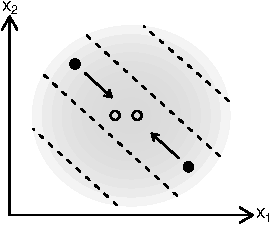
\includegraphics{trading-genetics_files/figure-latex/pic-intuition-1} }\subfloat[Children\label{fig:pic-intuition-2}]{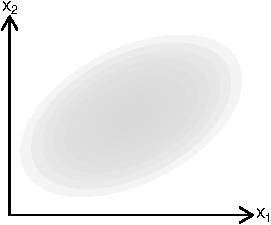
\includegraphics{trading-genetics_files/figure-latex/pic-intuition-2} }

}

\caption{Theory. The shaded area is the population distribution. Parents (solid circles) match along attractiveness isoquants (dotted lines). Children (hollow circles) are between them. As a result, in the children's generation, the distribution is squeezed along attractiveness isoquants.}\label{fig:pic-intuition}
\end{figure}

These results show that SGAM can lead to a genes-SES gradient, i.e.~a positive
correlation between genes and SES. Also, the strength of the genes-SES
correlation is affected by economic institutions, as captured in \(\theta\).
When \(\theta\) is high, the genes-SES correlation is high too.

We now consider the asymptotic distribution of \(x_1\) and \(x_2\) when the matching
process is repeated over many generations. As we would expect, our main results
continue to hold.

\begin{proposition}\label{prop-asymptotics-RM}
Under random matching, the dynamics converges to a stationary distribution that 
is normal with mean zero and covariance matrix 
\[
\mathbb{C}\left(\begin{array}{cc}
x_1  \\
x_2
\end{array}
\right)
=
\left( 
\begin{array}{cc}
\frac{2}{2-\tau ^{2}} & 0 \\ 
0 & \frac{2}{2-\theta ^{2}}%
\end{array}%
\right) \allowbreak 
\]%
In particular, the traits are asymptotically uncorrelated and children's
expected genetic endowment is independent of parents' wealth.

\end{proposition}

\begin{proposition}\label{prop-asymptotics-SGAM}
Under SGAM, for $\theta <1$ and $\tau <1$, the dynamics converge to a stationary
distribution that is normal with mean zero and covariance matrix 
\[
\mathbb{C}\left(\begin{array}{cc}
x_1  \\
x_2
\end{array}
\right)
=
\left(
\begin{array}{cc}
\bar{s}^{2} & \bar{\sigma} \\ 
\bar{\sigma} & \bar{S}^{2}%
\end{array}%
\right) 
\]
Moreover, the asymptotic correlation between characteristics, 
$corr = \bar{\sigma}/\bar{s}\bar{S}$, is non-negative, positive for $0 < a < 1$, 
increasing in $\theta$ and increasing then decreasing in $a$. 
The coefficient of parents' wealth on children's genetics is also positive 
for $0 < a < 1$.

For $\theta = 1$, the dynamics diverge and $\bar{S}^{2}$ goes to $+\infty$; for 
$\tau = 1$, the dynamics diverges and $\bar{s}^{2}$ goes to $+\infty$.

\end{proposition}

Figure \ref{fig:pic-asymptotic-corr} plots the asymptotic correlation
between \(x_1\) and \(x_2\) for \(\tau = 0.95\).

\begin{figure}

{\centering 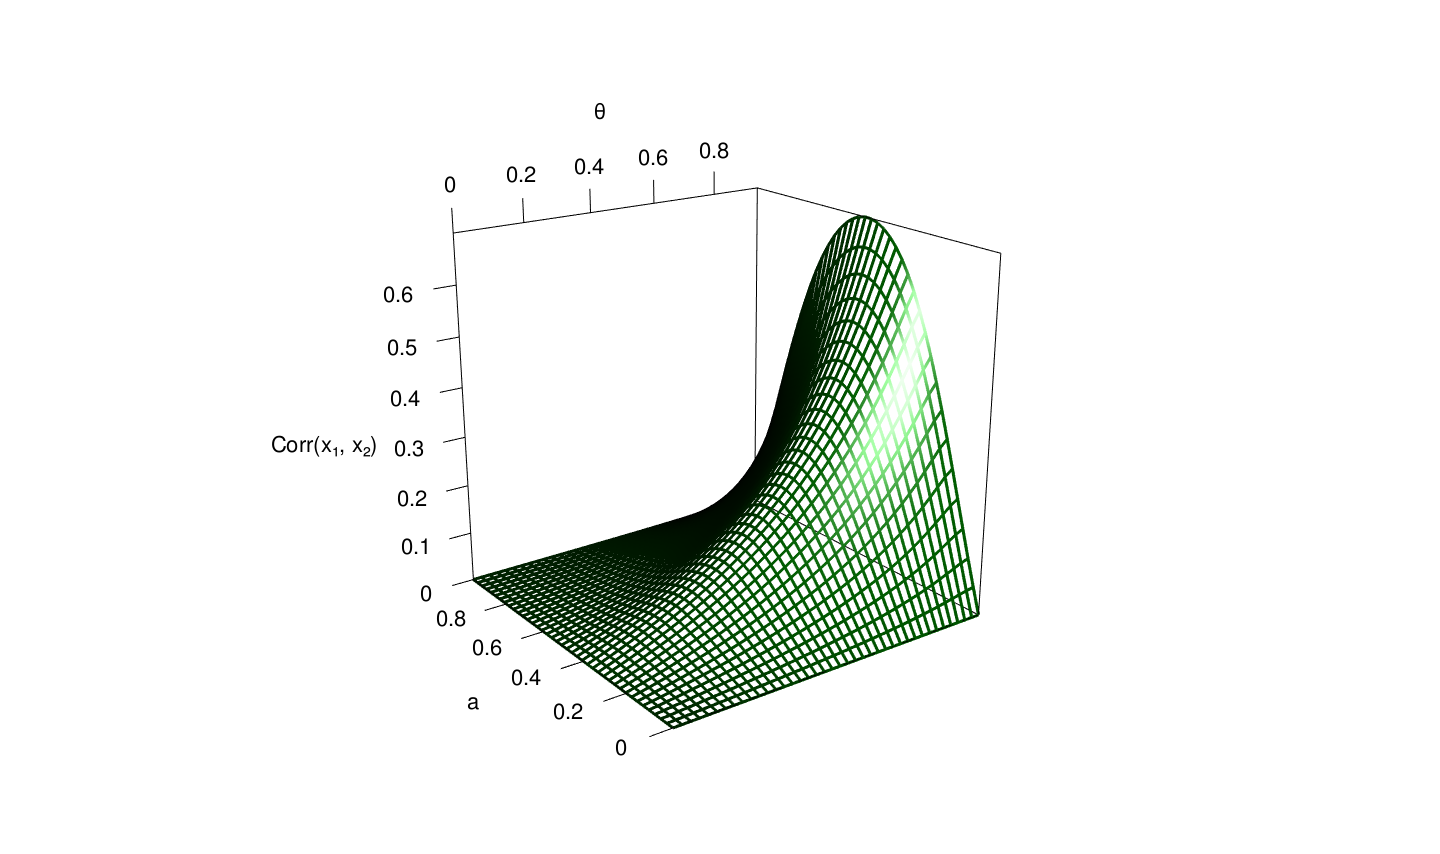
\includegraphics[height=3.5in]{trading-genetics_files/figure-latex/pic-asymptotic-corr-1-rgl} 

}

\caption{Long-run correlation between genetics $x_1$ and SES $x_2$, by weight of genetics in matching $a$ and SES inheritance $\theta$. $\tau$ = 0.95.}\label{fig:pic-asymptotic-corr}
\end{figure}

Note that both \(\bar{S}^{2}\) and \(\bar{\sigma}\), as well as the correlation
between characteristics and the conditional expectation of genetics given
wealth, are increasing in \(\theta\), i.e.~decreasing in the tax rate. Higher
taxation reduces the asymptotic variance of wealth (not surprisingly), but
also the correlation between genetics and wealth.

\hypertarget{extensions}{%
\subsection{Extensions}\label{extensions}}

We consider three extensions. First, the relative attractiveness of genes and
SES might differ for men and women. Our basic result extends to this setup.

\begin{claim}\label{claim-men-women-different}
Suppose that men's and women's attractiveness is given by
\begin{align*}
i(x) &= ax_1 + (1-a)x_2, \\
j(y) &= by_1 + (1-b)y_2
\end{align*}
respectively, with $0\le a \le 1$, $0 \le b \le 1$. Then if $\sigma = 0$, children's 
characteristics $x^\prime_1$ and $x^\prime_2$ will be positively correlated 
unless $a = b = 0$ or $a = b = 1$. The correlation is increasing in $\theta$.

\end{claim}

Interestingly, the \(x_1\)-\(x_2\) correlation is highest when \(a\) and \(b\) are most
different from each other. So gender differences in what counts as attractive
make the effects of SGAM stronger. Intuitively, if one sex only assorts on
SES while the other sex only assorts on genetics, this induces a very reliable
correlation between genes and SES in couples, since (e.g.) every high-SES male
is matched for sure with a high-genetics female.

Second, in modern meritocracies, people's adult SES depends not just
on their parents' social status and on chance, but also on their own effort and
skills, which might be related to their genetics. So, let
\begin{align}
x^\prime_1 &= \tau \frac{x_{1} + y_{1}}{2} + \varepsilon   \nonumber \\
x^\prime_2 &= \gamma x^\prime_1 + \theta \frac{x_{2}+y_{2}}{2}+\eta \label{eqn-gamma}
\end{align}
where \(\gamma > 0\) represents the effect of own genetics on own SES.
The basic result continues to hold, and also, the degree of meritocracy \(\gamma\)
increases the correlation between genes and SES; a highly meritocratic
society may in the long run lead to a highly unfair genes-SES gradient.

\begin{proposition}\label{prop-gamma}
Under SGAM and equation \eqref{eqn-gamma}, if genetics and SES are 
uncorrelated for the parents, then they
are positively correlated for the children so long as $0 < a < 1$ or
$\gamma > 0$. The correlation is increasing in $\gamma$. Also, so 
long as $\gamma > 0$ and either $0 < a < 1$ or $\sigma > 0$, the coefficient 
of parents' wealth on children's wealth exceeds $\theta$.
\end{proposition}

Surprisingly, in this case, the children's genes-SES correlation is not always
increasing in \(\theta\). The reason is that when \(\gamma\) is high, a higher
\(\theta\) decreases the proportion of \(x^\prime_2\) that comes via \(\gamma\) from
own genetics, and increases the proportion that comes from parents' SES, which
may be less strongly correlated with own genetics. Figure \ref{fig:pic-gamma}
plots the correlation for \(\gamma = 0.15\), by \(a\) and \(\theta\). However,
computing the asymptotic correlation shows that it is increasing in \(\theta\) for
all but values of \(\theta\) very close to 1.

\begin{figure}

{\centering 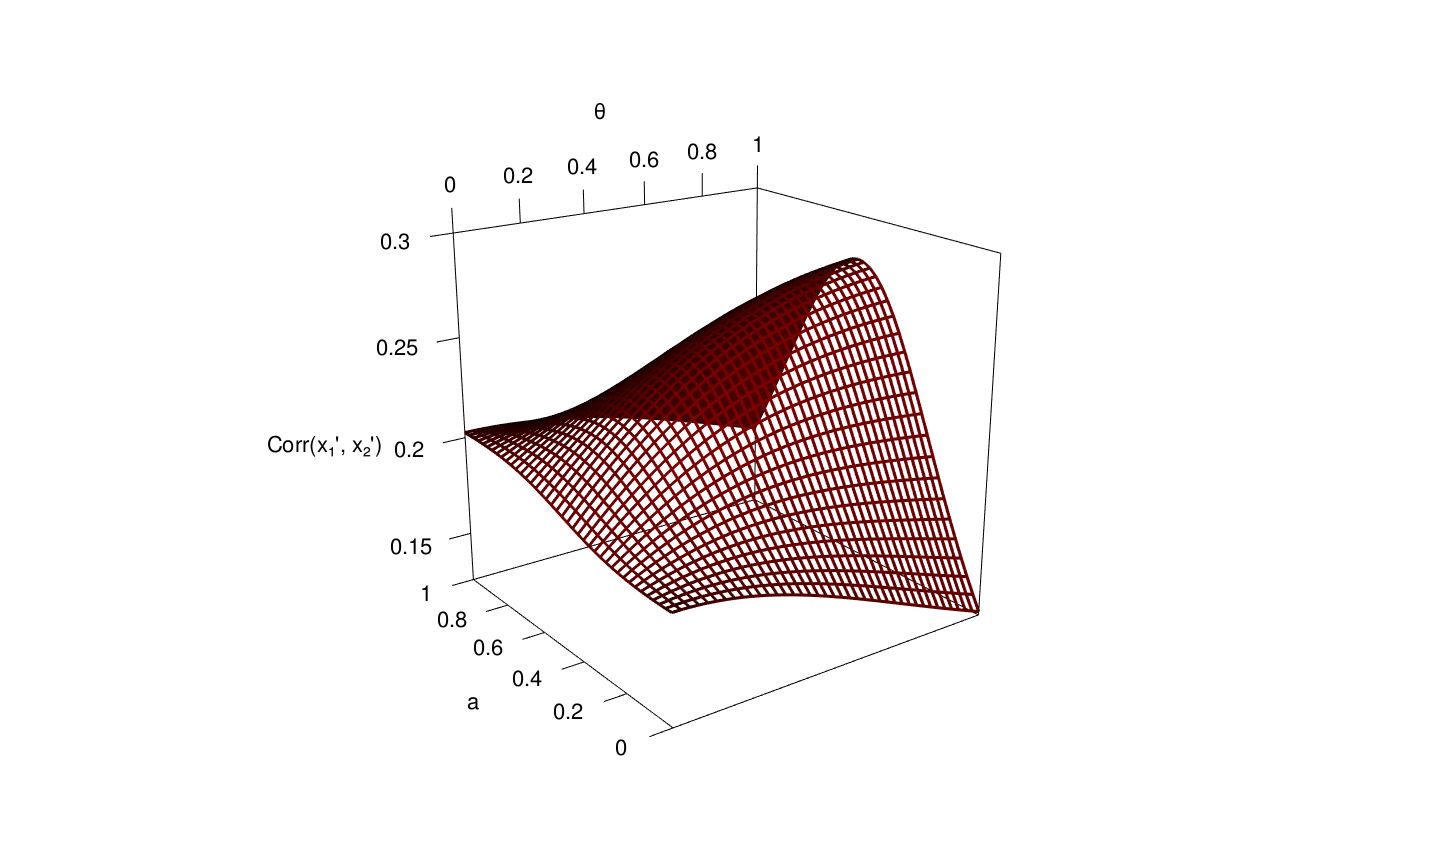
\includegraphics[height=3.5in]{trading-genetics_files/figure-latex/pic-gamma-2-rgl} 

}

\caption{Correlation between children's genetics $x^\prime_1$ and children's SES $x^\prime_2$, by weight of genetics in matching $a$ and SES inheritance $\theta$, for meritocracy $\gamma$ = 0.15. Other parameters: $\tau$ = 0.95, $s$ = $S$ = 1, $\sigma$ = 0.}\label{fig:pic-gamma}
\end{figure}

Third, we consider non-normal distributions of \(x_1\) and \(x_2\), non-normal
shocks \(\varepsilon\) and \(\eta\), and non-linear attractiveness functions. Suppose
\begin{equation}\label{non-linear-f} 
i(x) = f(ax_1, (1-a)x_2) 
\end{equation}
with \(f\) strictly increasing in both its arguments. Our sole condition on the
distribution of \(x\) is that a positive measure of the population has
attractiveness \(i(x) = i\) where the distribution of \((x_1, x_2)|i\) is
non-degenerate, i.e.~not everybody with attractiveness \(i\) is both genetically
and socially identical. In particular, this allows for discrete distributions,
like some kinds of social status.

\begin{proposition}\label{prop-non-normal}
Let attractiveness be given by \eqref{non-linear-f}. Let $(x_1, x_2)$ have
any distribution such that a positive measure of the population has
$i(x) = i$ where the conditional distribution of $(x_1, x_2)|i(x) = i$ is 
non-degenerate. Let $\eta$ and $\varepsilon$ be mean 0 and independent of
$x$ and each other. If genetics and SES are uncorrelated for the parents, then
the correlation among children is non-negative, and strictly positive if 
$0 < a < 1$.
\end{proposition}

Other extensions are possible. We assumed that all couples have the same number
of children. If fertility increased with \(x_1\) or \(x_2\), we would expect this to
reduce the variance of traits in the children's generation and possibly also
their covariance. Here, matching preferences, as summarized in the \(a\) parameter,
are exogenous. It would be natural to model \(a\) as an equilibrium outcome.
For example, if parents care about their children's wealth, \(a\) might decrease
in \(\theta\) and increase in \(\gamma\). Lastly, a gene-environment \emph{interaction}
(e.g.~\(x^\prime_2 = \gamma x^\prime_1 + \theta\frac{x_2+y_2}{2} + \zeta x'_1\frac{x_2+y_2}{2}\)) might increase the gene-environment
correlation some more.

\hypertarget{discussion}{%
\subsection{Discussion}\label{discussion}}

The meanings of both social status, and ``good genes'' in the
marriage market, are likely to vary across societies. Social status could
encompass variables like social class or caste; ethnic identity in
``ranked'' ethnic systems; or in modern societies, SES, including wealth, income
and occupation. Regarding genetics, standards of physical attractiveness, and
other genetically-influenced characteristics which make someone a ``good match'',
vary across societies and over time. The central prediction of the model is that
whatever those characteristics, in the long run they will become correlated with
SES.

Recent empirical work shows high persistence of SES over time, in particular at
the top. Clark (2021) argues that this is due to unobserved genetic variation.
Proposition \ref{prop-gamma} shows that if genes affect own wealth directly,
under assortative mating, the regression coefficient of parents' wealth on own
wealth exceeds the ``direct'' coefficient \(\theta\), because parents' wealth
correlates with parents' genetics and via that with own wealth. Thus,
regressions of wealth on wealth may include the effect of unobserved genetic
variation. This may be a confound due to pre-existing gene-SES correlation
(if \(\sigma > 0\)). But under SGAM it can also be a genuine cause, since changes
in someone's wealth may indeed affect the identity of their spouse, and therefore
the genetics of their offspring.

The converse also holds: regressions of children's characteristics on their
genetics alone risk overestimating the effect of genetics, by confounding it
with the effects of correlated socio-economic status. Recent work in genetics
has shown this. Polygenic scores for educational attainment have smaller effects
in between-sibling regressions, where between-family variation in SES is
partialled out and where genetic variants are guaranteed to be randomly
allocated, than in regressions which pool the whole sample (Howe et al. 2021).
Parents' genetic variants which are \emph{not} passed on to children predict
children's characteristics, via environmental effects (Kong et al. 2018).

The model predicts variation in the strength of SGAM. In particular, in
``caste societies'' where there is complete endogamy within social status
groups, there is no scope for SGAM, because marriage partners do not
trade off genetics for social status. Also, SGAM is increased by the institutional variable \(\theta\), which captures intergenerational persistence of SES. This
implies that policy has long-run effects on the social structure: reducing
\(\theta\) not only increases intergenerational mobility, but reduces
the correlation of genes with SES, and hence the unfairness of what
Harden (2021) calls the ``genetic lottery''.

\hypertarget{data-and-methods}{%
\section{Data and methods}\label{data-and-methods}}

In modern societies, both SGAM and meritocratic mobility may be at play. Genetic
variants that cause higher SES, e.g.~higher income and wealth,
will be passed down along with that status. At the same time, higher SES and ``good
genes'' will assort in the marriage market. To test this, we look at correlations
among spouses between one partner's SES and the other partner's genetics.

We use data from the UK Biobank, a study of about 500,000 individuals born
between 1935 and 1970 (Bycroft et al. 2018). The Biobank contains information on respondents'
genetics, derived from DNA microarrays, along with questionnaire data on health
and social outcomes. The Biobank does not contain explicit information on spouse
pairs. We categorize respondents as pairs if they:

\begin{itemize}
\tightlist
\item
  had the same home postcode on at least one occasion;\footnote{A typical UK postcode contains about 15 properties.}
\item
  both reported the same homeownership/renting status, length of time
  at the address, and number of children;
\item
  attended the same UK Biobank assessment center on the same day;
\item
  both reported living with their spouse (``husband, wife or partner'');
\item
  consisted of one male and one female.
\end{itemize}

We also eliminate all pairs where either spouse appeared more than once
in the data. This leaves a total of 35,682 pairs. Some of
these could be false positives, i.e.~people who are not each others'
spouse but simply live in the same postcode. To validate the accuracy of
our pairs, we use genetic relationships. Some respondents in the UK
Biobank sample have a child (inferred from genetic data) who is also in the
sample. Among our spouse pairs, 511 have a genetic
child of at least one partner in the sample. For 441 of
these, the child is the genetic child of both partners. If this
subsample is representative, then at least
86\% of the pairs who have had a
child, have had a child together. This is a lower bound, because those
who had a child with someone else may also have had a child with their partner
who is not in the UK Biobank sample. As a point of comparison, 11\% of families
with dependent children included a stepchild in England and Wales in
2011 (National Statistics 2014).

It is still possible that some pairs in our data may not be actual spouses. In
the appendix, to sign any possible bias in our estimates resulting from this, we
use a dataset of ``known fake'' pairs. We show that estimated coefficients of
interest are closer to zero among these fake pairs than among our candidate
``real pairs''. Because of this, any fake pairs remaining in our data are likely
to bias our coefficients towards zero.

Our key dependent variable is spouse's \emph{Polygenic Score for Educational
Attainment} (PSEA). A polygenic score is a DNA-derived summary measure
of genetic risk or propensity for a particular outcome, created from
summing small effects of many common genetic variants, known as Single
Nucleotide Polymorphisms (SNPs). We focus on PSEA rather than other
polygenic scores for two reasons. First, educational attainment plays a key role in
human mate search. People are attracted to educated potential partners
(Buss and Barnes 1986; Belot and Francesconi 2013); spouse pairs often have
similar levels of educational attainment, as well as similar PSEA
(Vandenberg 1972; Schwartz and Mare 2005; Greenwood et al. 2014; Hugh-Jones et al. 2016). Second, PSEA predicts a set of important socioeconomic
variables, including not only education but also social and geographic mobility,
IQ, future income and wealth (Belsky et al. 2016; Barth, Papageorge, and Thom 2020; Papageorge and Thom 2020).\footnote{See Papageorge and Thom (2020) for a detailed discussion of polygenic
  scores, aimed at economists.}

We calculate PSEA using per-SNP summary statistics from Lee et al. (2018),
re-estimated excluding UK Biobank participants.\footnote{PSEA was computed by summing the alleles across \textasciitilde1.3 million
  genetic variants weighted by their effect sizes as estimated in
  genome-wide association studies (GWASs) that excluded UK Biobank.
  PSEA was then residualized on the first 100 principal components of
  the SNP array data. Further details can be found in
  Abdellaoui et al. (2019).} We normalize the score to
have mean 0 and variance 1. Because polygenic scores are created from estimates
of many presumably tiny effects, they contain a large amount of noise relative
to the true best estimator that could be derived from genetic data. For
instance, PSEA explains only 11--13\% of variance in educational attainment (out
of sample, Lee et al. 2018), whereas the true proportion explained by genetic
variation -- the heritability -- is estimated from twin studies to be about 40\%
(Branigan, McCallum, and Freese 2013). In addition, polygenic scores are no more guaranteed
to be causal than any other independent variable. For example, social
stratification by ancestry may lead genes to be associated with educational
attainment even if they play no causal role (Selzam et al. 2019).

Despite these points, PSEA has non-trivial estimated effects on educational
attainment. PSEA correlates with measures of education, including university
attendance and years of full-time education; within-siblings regressions, where
PSEA is randomly assigned by the ``lottery of meiosis'', confirm this correlation
is at least partly causal (Lee et al. 2018). We recheck these facts within the UK
Biobank sample. In a simple linear regression (N = 408,524) of
university attendance on PSEA, a one-standard-deviation increase in PSEA was
associated with a 9.2 percentage point increase in the
probability of university attendance (\(p < 2 \times 10^{-16}\)). In a
within-siblings regression among genetic full siblings (N =
36,748), the increase was
4.5 percentage points (\(p < 2 \times 10^{-16}\)).
This suggests that about half of the raw correlation of PSEA with
university attendance is down to confounds like good environments or parental
nurture, while the remainder is causal. Still, the causal effect remains
substantial: for a rough comparison, the (ITT) effect on college attendance of
the Moving To Opportunity experiment in the US was 2.5 percentage points
(Chetty, Hendren, and Katz 2016).

We use two measures of socio-economic status: income, and university attendance.
Income is a direct measure of SES. University attendance is a predictor of
income over the whole life course, and a form of SES in itself. The UK Biobank
data only contains a direct measure of current household income, which is
inappropriate for our purposes because it includes income from both spouses and
is measured after marriage. Instead, we estimate income in £000s in the
respondent's first job, by matching the job's Standard Occupational
Classification (SOC) code with average earnings by SOC from National Statistics (2007). Job
codes are only available for a subset of 7681 respondents among
our pairs.

Figure \ref{fig:pic-basic-corr} illustrates the core idea of SGAM within our
pair data. The X axis shows a measure of one partner's socio-economic status:
university attendance or income. The Y axis plots the other partner's mean PSEA.
Both males and females who went to university had spouses with higher PSEA. So
did males and females with higher income in their first job. Since DNA is
inherited, these people's children will also have higher PSEA.

\begin{figure}

{\centering \subfloat[\label{fig:pic-basic-corr-1}]{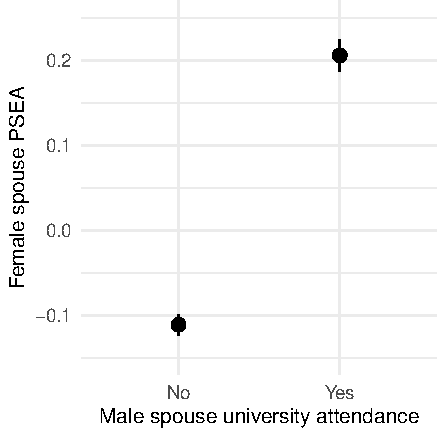
\includegraphics{trading-genetics_files/figure-latex/pic-basic-corr-1} }\subfloat[\label{fig:pic-basic-corr-2}]{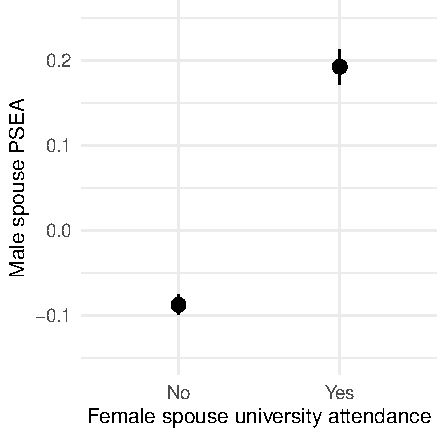
\includegraphics{trading-genetics_files/figure-latex/pic-basic-corr-2} }\newline\subfloat[\label{fig:pic-basic-corr-3}]{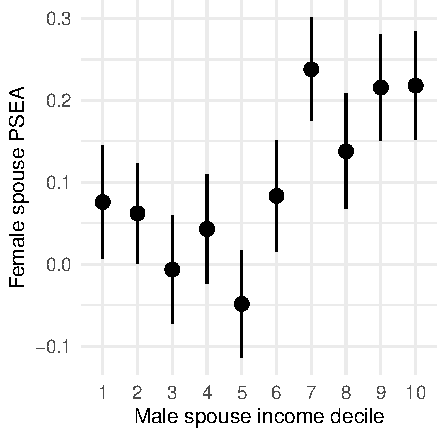
\includegraphics{trading-genetics_files/figure-latex/pic-basic-corr-3} }\subfloat[\label{fig:pic-basic-corr-4}]{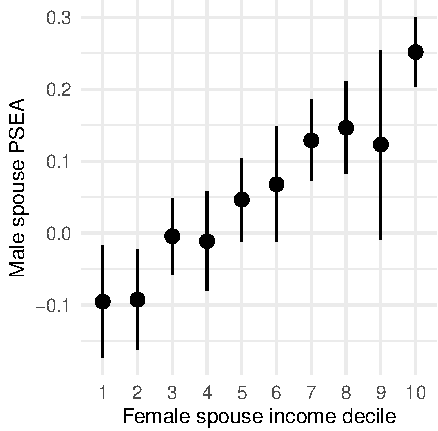
\includegraphics{trading-genetics_files/figure-latex/pic-basic-corr-4} }

}

\caption{Spouse PSEA against own university attendance and own income in first job. Lines show 95\% confidence intervals.}\label{fig:pic-basic-corr}
\end{figure}

These figures do not prove that SGAM is taking place. Since an
individual's own PSEA correlates with both their educational attainment,
and their income, both figures could be a result of genetic assortative
mating (GAM) alone (Hugh-Jones et al. 2016). Indeed, recent studies show much
higher levels of GAM than could be explained by matching on the observed
education phenotype alone (Okbay et al. 2022). So, to demonstrate SGAM, we need
a source of social status which is exogenous to genetics. Also, the link
between social status and spouse genetics is likely to be noisy, for
three reasons: first, polygenic scores contain a large amount of error, as
discussed above; second, causal mechanisms behind variation in social status
are likely to be noisy; third, to paraphrase Shakespeare (1595), the
spouse matching process is highly unpredictable. So, we need a large N to
give us sufficient power. This rules out time-limited shocks such as
changes to the school leaving age (Davies et al. 2018).

We use \emph{birth order}. It is known that earlier-born children receive more
parental care and have better life outcomes, including measures of SES such as
educational attainment and occupational status (Lindahl 2008; Booth and Kee 2009; Black, Devereux, and Salvanes 2011). On the other hand, all full siblings have the same \emph{ex ante}
expected genetic endowment from their parents, irrespective of their birth
order. This is guaranteed by the biological mechanism of meiosis, which ensures
that any gene is transmitted from either the mother or the father to the
child, with independent 50\% probability (Mendel 1865; Lawlor et al. 2008).
For example, siblings' expected polygenic score is equal to the mean of
their parents' polygenic scores.\footnote{Although genetic variation is randomly assigned to children at
  birth, genetics and birth order could be dependent if parents'
  choice of whether to have more children is endogenous to the genetic
  endowment of their earlier children. We check for this below.
  Isungset et al. (2021) also find that birth order differences in education are
  not genetic.} We can therefore use birth order as a
``shock'' to social status. We put ``shock'' in quotes because we do not claim that birth
order is exogenous to all other variables. For example, it naturally correlates
with parental age, and it may also correlate with household SES at the time of
birth. We only claim that birth order is exogenous to genetic variation.

Our main independent variable is respondents' birth order, i.e.~their
number of elder siblings plus one. For controls we use family size, i.e.
respondents' total number of siblings including themselves; month of birth; age
at interview; respondents' own PSEA; and their father's and/or mother's age
at their birth (calculated from parent's current age, only available if
the parent was still alive). For most regressions, we use only
respondents with between 1 and 5 siblings, i.e.~with a family size of
2-6.

\hypertarget{decomposing-the-birth-order-effect-on-spouse-genetics}{%
\subsection{Decomposing the birth order effect on spouse genetics}\label{decomposing-the-birth-order-effect-on-spouse-genetics}}

Ideally, we might prefer to use birth order as an instrument for SES. However,
our measures of social status are noisy and incomplete. For example, we know
whether subjects attended university, but not which university. Birth order
likely affects both measured and unmeasured aspects of SES. So, an instrumental
variables approach would be likely to fall foul of the exclusion restriction.

Instead, we conduct a mediation analysis, following the strategy of
Heckman, Pinto, and Savelyev (2013). We first confirm statistically that birth
order affects our measures of respondents' SES (income and education).
Then, we regress spouse's PSEA on birth order, with and without
controlling for SES. Under the assumption that birth order is exogenous
to own genetics, these regressions identify the effect of birth order,
plus other environmental variables that correlate with it, on own social
status and spouse's genetics. Also, if the estimated effect of birth
order on spouse's PSEA changes when SES is controlled for, that is
evidence that SES mediates the effect of birth order.

We follow Heckman, Pinto, and Savelyev (2013) to decompose the aggregate treatment
effect into components due to observed and unobserved proximate channels
affected by the treatment. Our aim is to estimate the effect of SES (as
an effect of birth order) on spouse PSEA.

Assume \(B\) is a multivalued variable indicating birth order. Let \(Y_b\) be
the counterfactual outcome (spouse PSEA) for the first-born, second-born etc.
Given \(b\), spouse PSEA is assumed to be independent across observations
conditional on some predetermined controls which are assumed not to be affected
by \(B\).

Let \(m_{b}\) be a set of mediators, i.e.~proximate outcomes
determined by \(b\), which account (at least in part) for the \(b\)
treatment effect on spouse PSEA. We can think of \(m_{b}\) as all
the effects on attractiveness, such as increments to SES, health,
cognitive and non-cognitive skills, that individuals receive due to
their birth rank. We can split the mediators in \(m_b\) into a set \(J_m\) of
measured mediators, including university attendance and income in first job,
and a set \(J_u\) of mediators that we cannot measure.

Our linear model is:

\begin{equation}
\label{eq:linear-model}
Y_b = \kappa_b + \sum_{j \in J_m} \alpha_b^j m^j_b+\sum_{j \in J_u} \alpha_b^j m^j_b + \mathbf{X^\prime} \symbf{\beta_b} + \tilde{\varepsilon}_b = \tau_b + \sum_{j \in J_m} \alpha_b^j m^j_b + \mathbf{X^\prime} \symbf{\beta_b} + \varepsilon_b 
\end{equation}

where \(\tilde{\varepsilon}_b\) is a mean-zero residual assumed independent of
\(m_b\) and \(\mathbf{X}\);
\(\tau_b = \kappa_b + \sum_{j \in J_u} \alpha_b^j E(m^j_b)\); and
\(\varepsilon_b = \tilde{\varepsilon}_b + \sum_{j \in J_u} (m^j_b - E(m^j_b))\).
We simplify by assuming that \(\beta_b = \beta\)
and \(\alpha_b = \alpha\) for all \(b\), i.e.~that the effects of \(\mathbf{X}\) and
\(m_B\) don't differ by birth order.\footnote{Under the assumption that measured and unmeasured mediators are
  uncorrelated, we can test these assumptions by running an OLS regression of an
  extended model \eqref{eq:model-to-estimate} where we interact the measured
  mediators and controls with the treatment \(B\), and test the significance of the
  coefficients on the interaction terms (\(\symbf{\alpha_b}=0\) and
  \(\symbf{\beta_b}=0\)). See Heckman, Pinto, and Savelyev (2013) and Fagereng, Mogstad, and Rønning (2021)
  for details and different applications. When we run the model with interactions,
  only one interaction is significant after Bonferroni correction at \(p < 0.05/34\):
  the interaction of income in first job with the dummy for birth order 6. So
  overall, the uninteracted model seems a good enough approximation.} We assume differences in
unmeasured investments due to \(b\) are independent of \(\mathbf{X}\).

We use a linear model for each observed mediator variable:
\begin{equation}
\label{eq:mediator-model}
m^j_b=\mu_{0,j}+\mathbf{X^\prime}\symbf{\mu_{1,j}}+\mu_{2,j}\cdot b+\eta_j, j \in J_m  
\end{equation}
where \(\eta_j\) is a mean-zero residual. We also assume the treatment-specific
intercepts are linear in \(b\):
\begin{equation}
\label{eq:linear-intercept}
\tau_b=\tau_{0}+\tau b.  
\end{equation}

With the simplifying assumptions above and substituting \eqref{eq:mediator-model}
and \eqref{eq:linear-intercept} into \eqref{eq:linear-model} we obtain:
\begin{equation}
\label{eq:simplified-model}
Y_b = \tau_0+\tau b + \sum_{j \in J_m} \alpha^j (\mu_{0,j}+\mathbf{X^\prime}\symbf{\mu_{1,j}}+\mu_{2,j}\cdot b+\eta_j) + \mathbf{X^\prime} \symbf{\beta} + \varepsilon_b 
\end{equation}

Using equation \eqref{eq:simplified-model}, we can decompose the average treatment
effect of a change from birth order \(b\) to \(b'\) into the effect of measured mediators
\(m^j\) and unmeasured mediators on the outcome:

\begin{equation}
\label{eq:decomposition}
E(Y_b' - Y_b) = \tau(b' - b) + \sum_{j \in J_m} \alpha^j E(m^j_{b'} - m^j_b) \\
=\underbrace{\tau(b' - b)}_{\text{Effect of unmeasured mediators}} + \underbrace{\sum_{j \in J_m} \alpha^j \mu_{2,j} (b' - b)}_{\text{Effect of measured mediators}}
\end{equation}

We are primarily interested in estimating the effect of SES on spouse PSEA,
amongst the measured mediators, and furthermore we would like to measure the
relative importance of SES compared to other factors in predicting spouse PSEA.

We therefore estimate:
\begin{equation}
\label{eq:model-to-estimate}
Y = \tau_0 + \tau B + \sum_{j \in J_m} \alpha^j m^j_b + \mathbf{X'} \symbf{\beta} + \varepsilon
\end{equation}

Estimating the above by OLS will generate unbiased estimates of
\(\alpha^j\) if \(m^j\) is measured without error and is
uncorrelated with the error term \(\varepsilon\). Since
\(\varepsilon\) contains both individual disturbances and differences
in unmeasured investments due to birth order, there are two identifying assumptions that need to hold for unbiased OLS estimates: (a) the measured investments
(specifically SES) should be independent of unmeasured investments
generated by birth order. Failing this, the estimates of \(\alpha^j\) will be
conflated with the effects of unmeasured investments. Second, (b) the measured
investments should be uncorrelated with other shocks \(\tilde{\varepsilon}_b\).

By running a least square regression of \eqref{eq:model-to-estimate}, we can
estimate \(\tau\) and \(\alpha^j\). If assumption (a) holds, the part of the birth
order treatment effect on spouse PSEA that is due to measured mediators,
including SES, can be constructed using the estimated \(\alpha^j\) and the effects
of birth order on measured mediators. We can estimate these effects in a second
step, from OLS regressions based on equation \eqref{eq:mediator-model} for each
measured mediator (in particular university attendance and income) on
\(\mathbf{X}\) and \(B\). The part of the birth order effect that is due to
university attendance (or income) on spouse PSEA will be the coefficient of
university/income in the regression of spouse PSEA in equation
\eqref{eq:model-to-estimate}, multiplied by the coefficient of birth order on
university/income from equation \eqref{eq:mediator-model}.

\hypertarget{results}{%
\section{Results}\label{results}}

 
  \providecommand{\huxb}[2]{\arrayrulecolor[RGB]{#1}\global\arrayrulewidth=#2pt}
  \providecommand{\huxvb}[2]{\color[RGB]{#1}\vrule width #2pt}
  \providecommand{\huxtpad}[1]{\rule{0pt}{#1}}
  \providecommand{\huxbpad}[1]{\rule[-#1]{0pt}{#1}}

\begin{table}[ht]
\begin{centerbox}
\begin{threeparttable}
\captionsetup{justification=centering,singlelinecheck=off}
\caption{\label{tab:tbl-bo-first-stage} Regressions of mediators on birth order}
 \setlength{\tabcolsep}{0pt}
\begin{tabularx}{1\textwidth}{p{0.142857142857143\textwidth} p{0.142857142857143\textwidth} p{0.142857142857143\textwidth} p{0.142857142857143\textwidth} p{0.142857142857143\textwidth} p{0.142857142857143\textwidth} p{0.142857142857143\textwidth}}


\hhline{>{\huxb{0, 0, 0}{0.8}}->{\huxb{0, 0, 0}{0.8}}->{\huxb{0, 0, 0}{0.8}}->{\huxb{0, 0, 0}{0.8}}->{\huxb{0, 0, 0}{0.8}}->{\huxb{0, 0, 0}{0.8}}->{\huxb{0, 0, 0}{0.8}}-}
\arrayrulecolor{black}

\multicolumn{1}{!{\huxvb{0, 0, 0}{0}}p{0.142857142857143\textwidth}!{\huxvb{0, 0, 0}{0}}}{\hspace{6pt}\parbox[b]{0.142857142857143\textwidth-6pt-6pt}{\huxtpad{6pt + 1em}\centering \huxbpad{6pt}}} &
\multicolumn{1}{p{0.142857142857143\textwidth}!{\huxvb{0, 0, 0}{0}}}{\hspace{6pt}\parbox[b]{0.142857142857143\textwidth-6pt-6pt}{\huxtpad{6pt + 1em}\centering University\huxbpad{6pt}}} &
\multicolumn{1}{p{0.142857142857143\textwidth}!{\huxvb{0, 0, 0}{0}}}{\hspace{6pt}\parbox[b]{0.142857142857143\textwidth-6pt-6pt}{\huxtpad{6pt + 1em}\centering Income\huxbpad{6pt}}} &
\multicolumn{1}{p{0.142857142857143\textwidth}!{\huxvb{0, 0, 0}{0}}}{\hspace{6pt}\parbox[b]{0.142857142857143\textwidth-6pt-6pt}{\huxtpad{6pt + 1em}\centering Fluid IQ\huxbpad{6pt}}} &
\multicolumn{1}{p{0.142857142857143\textwidth}!{\huxvb{0, 0, 0}{0}}}{\hspace{6pt}\parbox[b]{0.142857142857143\textwidth-6pt-6pt}{\huxtpad{6pt + 1em}\centering Height\huxbpad{6pt}}} &
\multicolumn{1}{p{0.142857142857143\textwidth}!{\huxvb{0, 0, 0}{0}}}{\hspace{6pt}\parbox[b]{0.142857142857143\textwidth-6pt-6pt}{\huxtpad{6pt + 1em}\centering BMI\huxbpad{6pt}}} &
\multicolumn{1}{p{0.142857142857143\textwidth}!{\huxvb{0, 0, 0}{0}}}{\hspace{6pt}\parbox[b]{0.142857142857143\textwidth-6pt-6pt}{\huxtpad{6pt + 1em}\centering Health\huxbpad{6pt}}} \tabularnewline[-0.5pt]


\hhline{>{\huxb{255, 255, 255}{0.4}}->{\huxb{0, 0, 0}{0.4}}->{\huxb{0, 0, 0}{0.4}}->{\huxb{0, 0, 0}{0.4}}->{\huxb{0, 0, 0}{0.4}}->{\huxb{0, 0, 0}{0.4}}->{\huxb{0, 0, 0}{0.4}}-}
\arrayrulecolor{black}

\multicolumn{1}{!{\huxvb{0, 0, 0}{0}}p{0.142857142857143\textwidth}!{\huxvb{0, 0, 0}{0}}}{\hspace{6pt}\parbox[b]{0.142857142857143\textwidth-6pt-6pt}{\huxtpad{6pt + 1em}\raggedright Birth order\huxbpad{6pt}}} &
\multicolumn{1}{p{0.142857142857143\textwidth}!{\huxvb{0, 0, 0}{0}}}{\hspace{6pt}\parbox[b]{0.142857142857143\textwidth-6pt-6pt}{\huxtpad{6pt + 1em}\raggedleft $-$0.0790 ***\huxbpad{6pt}}} &
\multicolumn{1}{p{0.142857142857143\textwidth}!{\huxvb{0, 0, 0}{0}}}{\hspace{6pt}\parbox[b]{0.142857142857143\textwidth-6pt-6pt}{\huxtpad{6pt + 1em}\raggedleft $-$1.0899 *\hphantom{0}\hphantom{0}\huxbpad{6pt}}} &
\multicolumn{1}{p{0.142857142857143\textwidth}!{\huxvb{0, 0, 0}{0}}}{\hspace{6pt}\parbox[b]{0.142857142857143\textwidth-6pt-6pt}{\huxtpad{6pt + 1em}\raggedleft $-$0.2733 ***\huxbpad{6pt}}} &
\multicolumn{1}{p{0.142857142857143\textwidth}!{\huxvb{0, 0, 0}{0}}}{\hspace{6pt}\parbox[b]{0.142857142857143\textwidth-6pt-6pt}{\huxtpad{6pt + 1em}\raggedleft $-$0.7012 ***\huxbpad{6pt}}} &
\multicolumn{1}{p{0.142857142857143\textwidth}!{\huxvb{0, 0, 0}{0}}}{\hspace{6pt}\parbox[b]{0.142857142857143\textwidth-6pt-6pt}{\huxtpad{6pt + 1em}\raggedleft 0.1907 **\hphantom{0}\huxbpad{6pt}}} &
\multicolumn{1}{p{0.142857142857143\textwidth}!{\huxvb{0, 0, 0}{0}}}{\hspace{6pt}\parbox[b]{0.142857142857143\textwidth-6pt-6pt}{\huxtpad{6pt + 1em}\raggedleft $-$0.0430 ***\huxbpad{6pt}}} \tabularnewline[-0.5pt]


\hhline{}
\arrayrulecolor{black}

\multicolumn{1}{!{\huxvb{0, 0, 0}{0}}p{0.142857142857143\textwidth}!{\huxvb{0, 0, 0}{0}}}{\hspace{6pt}\parbox[b]{0.142857142857143\textwidth-6pt-6pt}{\huxtpad{6pt + 1em}\raggedright \huxbpad{6pt}}} &
\multicolumn{1}{p{0.142857142857143\textwidth}!{\huxvb{0, 0, 0}{0}}}{\hspace{6pt}\parbox[b]{0.142857142857143\textwidth-6pt-6pt}{\huxtpad{6pt + 1em}\raggedleft (0.0067)\hphantom{0}\hphantom{0}\hphantom{0}\huxbpad{6pt}}} &
\multicolumn{1}{p{0.142857142857143\textwidth}!{\huxvb{0, 0, 0}{0}}}{\hspace{6pt}\parbox[b]{0.142857142857143\textwidth-6pt-6pt}{\huxtpad{6pt + 1em}\raggedleft (0.4264)\hphantom{0}\hphantom{0}\hphantom{0}\huxbpad{6pt}}} &
\multicolumn{1}{p{0.142857142857143\textwidth}!{\huxvb{0, 0, 0}{0}}}{\hspace{6pt}\parbox[b]{0.142857142857143\textwidth-6pt-6pt}{\huxtpad{6pt + 1em}\raggedleft (0.0304)\hphantom{0}\hphantom{0}\hphantom{0}\huxbpad{6pt}}} &
\multicolumn{1}{p{0.142857142857143\textwidth}!{\huxvb{0, 0, 0}{0}}}{\hspace{6pt}\parbox[b]{0.142857142857143\textwidth-6pt-6pt}{\huxtpad{6pt + 1em}\raggedleft (0.1355)\hphantom{0}\hphantom{0}\hphantom{0}\huxbpad{6pt}}} &
\multicolumn{1}{p{0.142857142857143\textwidth}!{\huxvb{0, 0, 0}{0}}}{\hspace{6pt}\parbox[b]{0.142857142857143\textwidth-6pt-6pt}{\huxtpad{6pt + 1em}\raggedleft (0.0662)\hphantom{0}\hphantom{0}\hphantom{0}\huxbpad{6pt}}} &
\multicolumn{1}{p{0.142857142857143\textwidth}!{\huxvb{0, 0, 0}{0}}}{\hspace{6pt}\parbox[b]{0.142857142857143\textwidth-6pt-6pt}{\huxtpad{6pt + 1em}\raggedleft (0.0103)\hphantom{0}\hphantom{0}\hphantom{0}\huxbpad{6pt}}} \tabularnewline[-0.5pt]


\hhline{}
\arrayrulecolor{black}

\multicolumn{1}{!{\huxvb{0, 0, 0}{0}}p{0.142857142857143\textwidth}!{\huxvb{0, 0, 0}{0}}}{\hspace{6pt}\parbox[b]{0.142857142857143\textwidth-6pt-6pt}{\huxtpad{6pt + 1em}\raggedright PSEA\huxbpad{6pt}}} &
\multicolumn{1}{p{0.142857142857143\textwidth}!{\huxvb{0, 0, 0}{0}}}{\hspace{6pt}\parbox[b]{0.142857142857143\textwidth-6pt-6pt}{\huxtpad{6pt + 1em}\raggedleft 0.0889 ***\huxbpad{6pt}}} &
\multicolumn{1}{p{0.142857142857143\textwidth}!{\huxvb{0, 0, 0}{0}}}{\hspace{6pt}\parbox[b]{0.142857142857143\textwidth-6pt-6pt}{\huxtpad{6pt + 1em}\raggedleft 1.5144 ***\huxbpad{6pt}}} &
\multicolumn{1}{p{0.142857142857143\textwidth}!{\huxvb{0, 0, 0}{0}}}{\hspace{6pt}\parbox[b]{0.142857142857143\textwidth-6pt-6pt}{\huxtpad{6pt + 1em}\raggedleft 0.3180 ***\huxbpad{6pt}}} &
\multicolumn{1}{p{0.142857142857143\textwidth}!{\huxvb{0, 0, 0}{0}}}{\hspace{6pt}\parbox[b]{0.142857142857143\textwidth-6pt-6pt}{\huxtpad{6pt + 1em}\raggedleft 0.1970 *\hphantom{0}\hphantom{0}\huxbpad{6pt}}} &
\multicolumn{1}{p{0.142857142857143\textwidth}!{\huxvb{0, 0, 0}{0}}}{\hspace{6pt}\parbox[b]{0.142857142857143\textwidth-6pt-6pt}{\huxtpad{6pt + 1em}\raggedleft $-$0.4281 ***\huxbpad{6pt}}} &
\multicolumn{1}{p{0.142857142857143\textwidth}!{\huxvb{0, 0, 0}{0}}}{\hspace{6pt}\parbox[b]{0.142857142857143\textwidth-6pt-6pt}{\huxtpad{6pt + 1em}\raggedleft 0.0533 ***\huxbpad{6pt}}} \tabularnewline[-0.5pt]


\hhline{}
\arrayrulecolor{black}

\multicolumn{1}{!{\huxvb{0, 0, 0}{0}}p{0.142857142857143\textwidth}!{\huxvb{0, 0, 0}{0}}}{\hspace{6pt}\parbox[b]{0.142857142857143\textwidth-6pt-6pt}{\huxtpad{6pt + 1em}\raggedright \huxbpad{6pt}}} &
\multicolumn{1}{p{0.142857142857143\textwidth}!{\huxvb{0, 0, 0}{0}}}{\hspace{6pt}\parbox[b]{0.142857142857143\textwidth-6pt-6pt}{\huxtpad{6pt + 1em}\raggedleft (0.0046)\hphantom{0}\hphantom{0}\hphantom{0}\huxbpad{6pt}}} &
\multicolumn{1}{p{0.142857142857143\textwidth}!{\huxvb{0, 0, 0}{0}}}{\hspace{6pt}\parbox[b]{0.142857142857143\textwidth-6pt-6pt}{\huxtpad{6pt + 1em}\raggedleft (0.3307)\hphantom{0}\hphantom{0}\hphantom{0}\huxbpad{6pt}}} &
\multicolumn{1}{p{0.142857142857143\textwidth}!{\huxvb{0, 0, 0}{0}}}{\hspace{6pt}\parbox[b]{0.142857142857143\textwidth-6pt-6pt}{\huxtpad{6pt + 1em}\raggedleft (0.0200)\hphantom{0}\hphantom{0}\hphantom{0}\huxbpad{6pt}}} &
\multicolumn{1}{p{0.142857142857143\textwidth}!{\huxvb{0, 0, 0}{0}}}{\hspace{6pt}\parbox[b]{0.142857142857143\textwidth-6pt-6pt}{\huxtpad{6pt + 1em}\raggedleft (0.0921)\hphantom{0}\hphantom{0}\hphantom{0}\huxbpad{6pt}}} &
\multicolumn{1}{p{0.142857142857143\textwidth}!{\huxvb{0, 0, 0}{0}}}{\hspace{6pt}\parbox[b]{0.142857142857143\textwidth-6pt-6pt}{\huxtpad{6pt + 1em}\raggedleft (0.0456)\hphantom{0}\hphantom{0}\hphantom{0}\huxbpad{6pt}}} &
\multicolumn{1}{p{0.142857142857143\textwidth}!{\huxvb{0, 0, 0}{0}}}{\hspace{6pt}\parbox[b]{0.142857142857143\textwidth-6pt-6pt}{\huxtpad{6pt + 1em}\raggedleft (0.0068)\hphantom{0}\hphantom{0}\hphantom{0}\huxbpad{6pt}}} \tabularnewline[-0.5pt]


\hhline{}
\arrayrulecolor{black}

\multicolumn{1}{!{\huxvb{0, 0, 0}{0}}p{0.142857142857143\textwidth}!{\huxvb{0, 0, 0}{0}}}{\hspace{6pt}\parbox[b]{0.142857142857143\textwidth-6pt-6pt}{\huxtpad{6pt + 1em}\raggedright Parents' age at birth\huxbpad{6pt}}} &
\multicolumn{1}{p{0.142857142857143\textwidth}!{\huxvb{0, 0, 0}{0}}}{\hspace{6pt}\parbox[b]{0.142857142857143\textwidth-6pt-6pt}{\huxtpad{6pt + 1em}\raggedleft 0.0163 ***\huxbpad{6pt}}} &
\multicolumn{1}{p{0.142857142857143\textwidth}!{\huxvb{0, 0, 0}{0}}}{\hspace{6pt}\parbox[b]{0.142857142857143\textwidth-6pt-6pt}{\huxtpad{6pt + 1em}\raggedleft 0.2623 ***\huxbpad{6pt}}} &
\multicolumn{1}{p{0.142857142857143\textwidth}!{\huxvb{0, 0, 0}{0}}}{\hspace{6pt}\parbox[b]{0.142857142857143\textwidth-6pt-6pt}{\huxtpad{6pt + 1em}\raggedleft 0.0588 ***\huxbpad{6pt}}} &
\multicolumn{1}{p{0.142857142857143\textwidth}!{\huxvb{0, 0, 0}{0}}}{\hspace{6pt}\parbox[b]{0.142857142857143\textwidth-6pt-6pt}{\huxtpad{6pt + 1em}\raggedleft 0.1514 ***\huxbpad{6pt}}} &
\multicolumn{1}{p{0.142857142857143\textwidth}!{\huxvb{0, 0, 0}{0}}}{\hspace{6pt}\parbox[b]{0.142857142857143\textwidth-6pt-6pt}{\huxtpad{6pt + 1em}\raggedleft $-$0.0989 ***\huxbpad{6pt}}} &
\multicolumn{1}{p{0.142857142857143\textwidth}!{\huxvb{0, 0, 0}{0}}}{\hspace{6pt}\parbox[b]{0.142857142857143\textwidth-6pt-6pt}{\huxtpad{6pt + 1em}\raggedleft 0.0110 ***\huxbpad{6pt}}} \tabularnewline[-0.5pt]


\hhline{}
\arrayrulecolor{black}

\multicolumn{1}{!{\huxvb{0, 0, 0}{0}}p{0.142857142857143\textwidth}!{\huxvb{0, 0, 0}{0}}}{\hspace{6pt}\parbox[b]{0.142857142857143\textwidth-6pt-6pt}{\huxtpad{6pt + 1em}\raggedright \huxbpad{6pt}}} &
\multicolumn{1}{p{0.142857142857143\textwidth}!{\huxvb{0, 0, 0}{0}}}{\hspace{6pt}\parbox[b]{0.142857142857143\textwidth-6pt-6pt}{\huxtpad{6pt + 1em}\raggedleft (0.0012)\hphantom{0}\hphantom{0}\hphantom{0}\huxbpad{6pt}}} &
\multicolumn{1}{p{0.142857142857143\textwidth}!{\huxvb{0, 0, 0}{0}}}{\hspace{6pt}\parbox[b]{0.142857142857143\textwidth-6pt-6pt}{\huxtpad{6pt + 1em}\raggedleft (0.0722)\hphantom{0}\hphantom{0}\hphantom{0}\huxbpad{6pt}}} &
\multicolumn{1}{p{0.142857142857143\textwidth}!{\huxvb{0, 0, 0}{0}}}{\hspace{6pt}\parbox[b]{0.142857142857143\textwidth-6pt-6pt}{\huxtpad{6pt + 1em}\raggedleft (0.0053)\hphantom{0}\hphantom{0}\hphantom{0}\huxbpad{6pt}}} &
\multicolumn{1}{p{0.142857142857143\textwidth}!{\huxvb{0, 0, 0}{0}}}{\hspace{6pt}\parbox[b]{0.142857142857143\textwidth-6pt-6pt}{\huxtpad{6pt + 1em}\raggedleft (0.0241)\hphantom{0}\hphantom{0}\hphantom{0}\huxbpad{6pt}}} &
\multicolumn{1}{p{0.142857142857143\textwidth}!{\huxvb{0, 0, 0}{0}}}{\hspace{6pt}\parbox[b]{0.142857142857143\textwidth-6pt-6pt}{\huxtpad{6pt + 1em}\raggedleft (0.0117)\hphantom{0}\hphantom{0}\hphantom{0}\huxbpad{6pt}}} &
\multicolumn{1}{p{0.142857142857143\textwidth}!{\huxvb{0, 0, 0}{0}}}{\hspace{6pt}\parbox[b]{0.142857142857143\textwidth-6pt-6pt}{\huxtpad{6pt + 1em}\raggedleft (0.0018)\hphantom{0}\hphantom{0}\hphantom{0}\huxbpad{6pt}}} \tabularnewline[-0.5pt]


\hhline{>{\huxb{255, 255, 255}{0.4}}->{\huxb{0, 0, 0}{0.4}}->{\huxb{0, 0, 0}{0.4}}->{\huxb{0, 0, 0}{0.4}}->{\huxb{0, 0, 0}{0.4}}->{\huxb{0, 0, 0}{0.4}}->{\huxb{0, 0, 0}{0.4}}-}
\arrayrulecolor{black}

\multicolumn{1}{!{\huxvb{0, 0, 0}{0}}p{0.142857142857143\textwidth}!{\huxvb{0, 0, 0}{0}}}{\hspace{6pt}\parbox[b]{0.142857142857143\textwidth-6pt-6pt}{\huxtpad{6pt + 1em}\raggedright Family size dummies\huxbpad{6pt}}} &
\multicolumn{1}{p{0.142857142857143\textwidth}!{\huxvb{0, 0, 0}{0}}}{\hspace{6pt}\parbox[b]{0.142857142857143\textwidth-6pt-6pt}{\huxtpad{6pt + 1em}\centering Yes\huxbpad{6pt}}} &
\multicolumn{1}{p{0.142857142857143\textwidth}!{\huxvb{0, 0, 0}{0}}}{\hspace{6pt}\parbox[b]{0.142857142857143\textwidth-6pt-6pt}{\huxtpad{6pt + 1em}\centering Yes\huxbpad{6pt}}} &
\multicolumn{1}{p{0.142857142857143\textwidth}!{\huxvb{0, 0, 0}{0}}}{\hspace{6pt}\parbox[b]{0.142857142857143\textwidth-6pt-6pt}{\huxtpad{6pt + 1em}\centering Yes\huxbpad{6pt}}} &
\multicolumn{1}{p{0.142857142857143\textwidth}!{\huxvb{0, 0, 0}{0}}}{\hspace{6pt}\parbox[b]{0.142857142857143\textwidth-6pt-6pt}{\huxtpad{6pt + 1em}\centering Yes\huxbpad{6pt}}} &
\multicolumn{1}{p{0.142857142857143\textwidth}!{\huxvb{0, 0, 0}{0}}}{\hspace{6pt}\parbox[b]{0.142857142857143\textwidth-6pt-6pt}{\huxtpad{6pt + 1em}\centering Yes\huxbpad{6pt}}} &
\multicolumn{1}{p{0.142857142857143\textwidth}!{\huxvb{0, 0, 0}{0}}}{\hspace{6pt}\parbox[b]{0.142857142857143\textwidth-6pt-6pt}{\huxtpad{6pt + 1em}\centering Yes\huxbpad{6pt}}} \tabularnewline[-0.5pt]


\hhline{}
\arrayrulecolor{black}

\multicolumn{1}{!{\huxvb{0, 0, 0}{0}}p{0.142857142857143\textwidth}!{\huxvb{0, 0, 0}{0}}}{\hspace{6pt}\parbox[b]{0.142857142857143\textwidth-6pt-6pt}{\huxtpad{6pt + 1em}\raggedright Birth month dummies\huxbpad{6pt}}} &
\multicolumn{1}{p{0.142857142857143\textwidth}!{\huxvb{0, 0, 0}{0}}}{\hspace{6pt}\parbox[b]{0.142857142857143\textwidth-6pt-6pt}{\huxtpad{6pt + 1em}\centering Yes\huxbpad{6pt}}} &
\multicolumn{1}{p{0.142857142857143\textwidth}!{\huxvb{0, 0, 0}{0}}}{\hspace{6pt}\parbox[b]{0.142857142857143\textwidth-6pt-6pt}{\huxtpad{6pt + 1em}\centering Yes\huxbpad{6pt}}} &
\multicolumn{1}{p{0.142857142857143\textwidth}!{\huxvb{0, 0, 0}{0}}}{\hspace{6pt}\parbox[b]{0.142857142857143\textwidth-6pt-6pt}{\huxtpad{6pt + 1em}\centering Yes\huxbpad{6pt}}} &
\multicolumn{1}{p{0.142857142857143\textwidth}!{\huxvb{0, 0, 0}{0}}}{\hspace{6pt}\parbox[b]{0.142857142857143\textwidth-6pt-6pt}{\huxtpad{6pt + 1em}\centering Yes\huxbpad{6pt}}} &
\multicolumn{1}{p{0.142857142857143\textwidth}!{\huxvb{0, 0, 0}{0}}}{\hspace{6pt}\parbox[b]{0.142857142857143\textwidth-6pt-6pt}{\huxtpad{6pt + 1em}\centering Yes\huxbpad{6pt}}} &
\multicolumn{1}{p{0.142857142857143\textwidth}!{\huxvb{0, 0, 0}{0}}}{\hspace{6pt}\parbox[b]{0.142857142857143\textwidth-6pt-6pt}{\huxtpad{6pt + 1em}\centering Yes\huxbpad{6pt}}} \tabularnewline[-0.5pt]


\hhline{}
\arrayrulecolor{black}

\multicolumn{1}{!{\huxvb{0, 0, 0}{0}}p{0.142857142857143\textwidth}!{\huxvb{0, 0, 0}{0}}}{\hspace{6pt}\parbox[b]{0.142857142857143\textwidth-6pt-6pt}{\huxtpad{6pt + 1em}\raggedright Birth year dummies\huxbpad{6pt}}} &
\multicolumn{1}{p{0.142857142857143\textwidth}!{\huxvb{0, 0, 0}{0}}}{\hspace{6pt}\parbox[b]{0.142857142857143\textwidth-6pt-6pt}{\huxtpad{6pt + 1em}\centering Yes\huxbpad{6pt}}} &
\multicolumn{1}{p{0.142857142857143\textwidth}!{\huxvb{0, 0, 0}{0}}}{\hspace{6pt}\parbox[b]{0.142857142857143\textwidth-6pt-6pt}{\huxtpad{6pt + 1em}\centering Yes\huxbpad{6pt}}} &
\multicolumn{1}{p{0.142857142857143\textwidth}!{\huxvb{0, 0, 0}{0}}}{\hspace{6pt}\parbox[b]{0.142857142857143\textwidth-6pt-6pt}{\huxtpad{6pt + 1em}\centering Yes\huxbpad{6pt}}} &
\multicolumn{1}{p{0.142857142857143\textwidth}!{\huxvb{0, 0, 0}{0}}}{\hspace{6pt}\parbox[b]{0.142857142857143\textwidth-6pt-6pt}{\huxtpad{6pt + 1em}\centering Yes\huxbpad{6pt}}} &
\multicolumn{1}{p{0.142857142857143\textwidth}!{\huxvb{0, 0, 0}{0}}}{\hspace{6pt}\parbox[b]{0.142857142857143\textwidth-6pt-6pt}{\huxtpad{6pt + 1em}\centering Yes\huxbpad{6pt}}} &
\multicolumn{1}{p{0.142857142857143\textwidth}!{\huxvb{0, 0, 0}{0}}}{\hspace{6pt}\parbox[b]{0.142857142857143\textwidth-6pt-6pt}{\huxtpad{6pt + 1em}\centering Yes\huxbpad{6pt}}} \tabularnewline[-0.5pt]


\hhline{>{\huxb{255, 255, 255}{0.4}}->{\huxb{0, 0, 0}{0.4}}->{\huxb{0, 0, 0}{0.4}}->{\huxb{0, 0, 0}{0.4}}->{\huxb{0, 0, 0}{0.4}}->{\huxb{0, 0, 0}{0.4}}->{\huxb{0, 0, 0}{0.4}}-}
\arrayrulecolor{black}

\multicolumn{1}{!{\huxvb{0, 0, 0}{0}}p{0.142857142857143\textwidth}!{\huxvb{0, 0, 0}{0}}}{\hspace{6pt}\parbox[b]{0.142857142857143\textwidth-6pt-6pt}{\huxtpad{6pt + 1em}\raggedright N\huxbpad{6pt}}} &
\multicolumn{1}{p{0.142857142857143\textwidth}!{\huxvb{0, 0, 0}{0}}}{\hspace{6pt}\parbox[b]{0.142857142857143\textwidth-6pt-6pt}{\huxtpad{6pt + 1em}\raggedleft 10220\hphantom{0}\hphantom{0}\hphantom{0}\hphantom{0}\hphantom{0}\hphantom{0}\hphantom{0}\hphantom{0}\hphantom{0}\huxbpad{6pt}}} &
\multicolumn{1}{p{0.142857142857143\textwidth}!{\huxvb{0, 0, 0}{0}}}{\hspace{6pt}\parbox[b]{0.142857142857143\textwidth-6pt-6pt}{\huxtpad{6pt + 1em}\raggedleft 3412\hphantom{0}\hphantom{0}\hphantom{0}\hphantom{0}\hphantom{0}\hphantom{0}\hphantom{0}\hphantom{0}\hphantom{0}\huxbpad{6pt}}} &
\multicolumn{1}{p{0.142857142857143\textwidth}!{\huxvb{0, 0, 0}{0}}}{\hspace{6pt}\parbox[b]{0.142857142857143\textwidth-6pt-6pt}{\huxtpad{6pt + 1em}\raggedleft 10220\hphantom{0}\hphantom{0}\hphantom{0}\hphantom{0}\hphantom{0}\hphantom{0}\hphantom{0}\hphantom{0}\hphantom{0}\huxbpad{6pt}}} &
\multicolumn{1}{p{0.142857142857143\textwidth}!{\huxvb{0, 0, 0}{0}}}{\hspace{6pt}\parbox[b]{0.142857142857143\textwidth-6pt-6pt}{\huxtpad{6pt + 1em}\raggedleft 10220\hphantom{0}\hphantom{0}\hphantom{0}\hphantom{0}\hphantom{0}\hphantom{0}\hphantom{0}\hphantom{0}\hphantom{0}\huxbpad{6pt}}} &
\multicolumn{1}{p{0.142857142857143\textwidth}!{\huxvb{0, 0, 0}{0}}}{\hspace{6pt}\parbox[b]{0.142857142857143\textwidth-6pt-6pt}{\huxtpad{6pt + 1em}\raggedleft 10220\hphantom{0}\hphantom{0}\hphantom{0}\hphantom{0}\hphantom{0}\hphantom{0}\hphantom{0}\hphantom{0}\hphantom{0}\huxbpad{6pt}}} &
\multicolumn{1}{p{0.142857142857143\textwidth}!{\huxvb{0, 0, 0}{0}}}{\hspace{6pt}\parbox[b]{0.142857142857143\textwidth-6pt-6pt}{\huxtpad{6pt + 1em}\raggedleft 10220\hphantom{0}\hphantom{0}\hphantom{0}\hphantom{0}\hphantom{0}\hphantom{0}\hphantom{0}\hphantom{0}\hphantom{0}\huxbpad{6pt}}} \tabularnewline[-0.5pt]


\hhline{}
\arrayrulecolor{black}

\multicolumn{1}{!{\huxvb{0, 0, 0}{0}}p{0.142857142857143\textwidth}!{\huxvb{0, 0, 0}{0}}}{\hspace{6pt}\parbox[b]{0.142857142857143\textwidth-6pt-6pt}{\huxtpad{6pt + 1em}\raggedright R2\huxbpad{6pt}}} &
\multicolumn{1}{p{0.142857142857143\textwidth}!{\huxvb{0, 0, 0}{0}}}{\hspace{6pt}\parbox[b]{0.142857142857143\textwidth-6pt-6pt}{\huxtpad{6pt + 1em}\raggedleft 0.074\hphantom{0}\hphantom{0}\hphantom{0}\hphantom{0}\hphantom{0}\huxbpad{6pt}}} &
\multicolumn{1}{p{0.142857142857143\textwidth}!{\huxvb{0, 0, 0}{0}}}{\hspace{6pt}\parbox[b]{0.142857142857143\textwidth-6pt-6pt}{\huxtpad{6pt + 1em}\raggedleft 0.026\hphantom{0}\hphantom{0}\hphantom{0}\hphantom{0}\hphantom{0}\huxbpad{6pt}}} &
\multicolumn{1}{p{0.142857142857143\textwidth}!{\huxvb{0, 0, 0}{0}}}{\hspace{6pt}\parbox[b]{0.142857142857143\textwidth-6pt-6pt}{\huxtpad{6pt + 1em}\raggedleft 0.058\hphantom{0}\hphantom{0}\hphantom{0}\hphantom{0}\hphantom{0}\huxbpad{6pt}}} &
\multicolumn{1}{p{0.142857142857143\textwidth}!{\huxvb{0, 0, 0}{0}}}{\hspace{6pt}\parbox[b]{0.142857142857143\textwidth-6pt-6pt}{\huxtpad{6pt + 1em}\raggedleft 0.017\hphantom{0}\hphantom{0}\hphantom{0}\hphantom{0}\hphantom{0}\huxbpad{6pt}}} &
\multicolumn{1}{p{0.142857142857143\textwidth}!{\huxvb{0, 0, 0}{0}}}{\hspace{6pt}\parbox[b]{0.142857142857143\textwidth-6pt-6pt}{\huxtpad{6pt + 1em}\raggedleft 0.023\hphantom{0}\hphantom{0}\hphantom{0}\hphantom{0}\hphantom{0}\huxbpad{6pt}}} &
\multicolumn{1}{p{0.142857142857143\textwidth}!{\huxvb{0, 0, 0}{0}}}{\hspace{6pt}\parbox[b]{0.142857142857143\textwidth-6pt-6pt}{\huxtpad{6pt + 1em}\raggedleft 0.018\hphantom{0}\hphantom{0}\hphantom{0}\hphantom{0}\hphantom{0}\huxbpad{6pt}}} \tabularnewline[-0.5pt]


\hhline{>{\huxb{0, 0, 0}{0.8}}->{\huxb{0, 0, 0}{0.8}}->{\huxb{0, 0, 0}{0.8}}->{\huxb{0, 0, 0}{0.8}}->{\huxb{0, 0, 0}{0.8}}->{\huxb{0, 0, 0}{0.8}}->{\huxb{0, 0, 0}{0.8}}-}
\arrayrulecolor{black}

\multicolumn{7}{!{\huxvb{0, 0, 0}{0}}p{1\textwidth+12\tabcolsep}!{\huxvb{0, 0, 0}{0}}}{\hspace{6pt}\parbox[b]{1\textwidth+12\tabcolsep-6pt-6pt}{\huxtpad{6pt + 1em}\raggedright Estimates from OLS regressions with the  mediators (university attendance, income, fluid IQ, height, BMI, self-reported health) as dependent variables, and own birth order as the main independent variable. PSEA is the polygenic score for educational attainment, which is normalized with mean 0 and standard deviation 1. We include parents' age at birth (the mean of parents' ages) and further controls to ensure the balance of covariates across birth order. All data is from the UK Biobank for a sample of UK individuals born between 1935 and 1970.  *** p $<$ 0.001;  ** p $<$ 0.01;  * p $<$ 0.05;  + p $<$ 0.1. Standard errors: robust.\huxbpad{6pt}}} \tabularnewline[-0.5pt]


\hhline{}
\arrayrulecolor{black}
\end{tabularx}
\end{threeparttable}\par\end{centerbox}

\end{table}
 

We first regress our measures of socio-economic status, university attendance
and income from first job, on birth order in our sample. We also do the same for
four non-SES mediators that could be affected by birth order: fluid IQ, height,
body mass index (BMI) and a measure of self-reported health. We control for
respondent's own PSEA and their parents' age at birth (see below). Table
\ref{tab:tbl-bo-first-stage} shows that birth order significantly predicts all
these variables. Effect sizes are quite substantial: on average, one extra elder
sibling reduces the chance of attending university by about
7.9 percentage points, income by about
£1,089, fluid IQ by about
0.27 points on a 13 point test, height by about
0.7 centimeters, and self reported health by
0.043 points on a 4-point scale; and increases BMI by
0.19.

Next we run regressions of spouse PSEA on birth order, within our dataset of
spouse pairs. Table \ref{tab:tbl-bo-psea-basic} reports the results. Column 1
reports results controlling only for family size (using dummies). As expected,
higher birth order is negatively associated with spouse's PSEA, though the
estimated effect size is small and insignificant. Column 2 reports results
controlling for the respondent's own PSEA, as well as dummies for birth year to
control for cohort effects, and dummies for birth month to control for
seasonal effects. The effect size of birth order is not much changed.

Column 3 reports results controlling for parents' age at birth. Within a family,
later children have older parents by definition. Older parents have more life
experience and may have higher income, which would presumably help later
children.\footnote{We often only have data only for one parent. We use this, or take the mean
  if we have both. There are also potential genetic effects from parental age,
  though recent research has rejected these in favour of ``social'' explanations
  (Kristensen and Bjerkedal 2007; Black, Devereux, and Salvanes 2011). Cochran and Harpending (2013) report that
  mutational load is approximately linear in father's age, while it is constant in
  mother's age. We observe very similar results if we control only for father's
  age at respondent's birth.} Including parents' age means we can separate the effect of
parental age from birth order. This reduces the N by a lot, since only
respondents with a live parent reported the necessary data. However, the effect
of birth order jumps in size and becomes significant at the 5 per cent level.
Meanwhile, parents' age has a positive effect. This suggests that estimates in
columns 1-2 mixed two opposite-signed effects: having older parents versus being
later in birth order.

 
  \providecommand{\huxb}[2]{\arrayrulecolor[RGB]{#1}\global\arrayrulewidth=#2pt}
  \providecommand{\huxvb}[2]{\color[RGB]{#1}\vrule width #2pt}
  \providecommand{\huxtpad}[1]{\rule{0pt}{#1}}
  \providecommand{\huxbpad}[1]{\rule[-#1]{0pt}{#1}}

\begin{table}[ht]
\begin{centerbox}
\begin{threeparttable}
\captionsetup{justification=centering,singlelinecheck=off}
\caption{\label{tab:tbl-bo-psea-basic} Regressions of spouse PSEA on birth order}
 \setlength{\tabcolsep}{0pt}
\begin{tabularx}{0.9\textwidth}{p{0.225\textwidth} p{0.225\textwidth} p{0.225\textwidth} p{0.225\textwidth}}


\hhline{>{\huxb{0, 0, 0}{0.8}}->{\huxb{0, 0, 0}{0.8}}->{\huxb{0, 0, 0}{0.8}}->{\huxb{0, 0, 0}{0.8}}-}
\arrayrulecolor{black}

\multicolumn{1}{!{\huxvb{0, 0, 0}{0}}p{0.225\textwidth}!{\huxvb{0, 0, 0}{0}}}{\hspace{6pt}\parbox[b]{0.225\textwidth-6pt-6pt}{\huxtpad{6pt + 1em}\centering \huxbpad{6pt}}} &
\multicolumn{1}{p{0.225\textwidth}!{\huxvb{0, 0, 0}{0}}}{\hspace{6pt}\parbox[b]{0.225\textwidth-6pt-6pt}{\huxtpad{6pt + 1em}\centering (1)\huxbpad{6pt}}} &
\multicolumn{1}{p{0.225\textwidth}!{\huxvb{0, 0, 0}{0}}}{\hspace{6pt}\parbox[b]{0.225\textwidth-6pt-6pt}{\huxtpad{6pt + 1em}\centering (2)\huxbpad{6pt}}} &
\multicolumn{1}{p{0.225\textwidth}!{\huxvb{0, 0, 0}{0}}}{\hspace{6pt}\parbox[b]{0.225\textwidth-6pt-6pt}{\huxtpad{6pt + 1em}\centering (3)\huxbpad{6pt}}} \tabularnewline[-0.5pt]


\hhline{>{\huxb{255, 255, 255}{0.4}}->{\huxb{0, 0, 0}{0.4}}->{\huxb{0, 0, 0}{0.4}}->{\huxb{0, 0, 0}{0.4}}-}
\arrayrulecolor{black}

\multicolumn{1}{!{\huxvb{0, 0, 0}{0}}p{0.225\textwidth}!{\huxvb{0, 0, 0}{0}}}{\hspace{6pt}\parbox[b]{0.225\textwidth-6pt-6pt}{\huxtpad{6pt + 1em}\raggedright Birth order\huxbpad{6pt}}} &
\multicolumn{1}{p{0.225\textwidth}!{\huxvb{0, 0, 0}{0}}}{\hspace{6pt}\parbox[b]{0.225\textwidth-6pt-6pt}{\huxtpad{6pt + 1em}\raggedleft $-$0.0091\hphantom{0}\huxbpad{6pt}}} &
\multicolumn{1}{p{0.225\textwidth}!{\huxvb{0, 0, 0}{0}}}{\hspace{6pt}\parbox[b]{0.225\textwidth-6pt-6pt}{\huxtpad{6pt + 1em}\raggedleft $-$0.0075\hphantom{0}\hphantom{0}\hphantom{0}\hphantom{0}\huxbpad{6pt}}} &
\multicolumn{1}{p{0.225\textwidth}!{\huxvb{0, 0, 0}{0}}}{\hspace{6pt}\parbox[b]{0.225\textwidth-6pt-6pt}{\huxtpad{6pt + 1em}\raggedleft $-$0.0314 *\hphantom{0}\hphantom{0}\huxbpad{6pt}}} \tabularnewline[-0.5pt]


\hhline{}
\arrayrulecolor{black}

\multicolumn{1}{!{\huxvb{0, 0, 0}{0}}p{0.225\textwidth}!{\huxvb{0, 0, 0}{0}}}{\hspace{6pt}\parbox[b]{0.225\textwidth-6pt-6pt}{\huxtpad{6pt + 1em}\raggedright \huxbpad{6pt}}} &
\multicolumn{1}{p{0.225\textwidth}!{\huxvb{0, 0, 0}{0}}}{\hspace{6pt}\parbox[b]{0.225\textwidth-6pt-6pt}{\huxtpad{6pt + 1em}\raggedleft (0.0074)\huxbpad{6pt}}} &
\multicolumn{1}{p{0.225\textwidth}!{\huxvb{0, 0, 0}{0}}}{\hspace{6pt}\parbox[b]{0.225\textwidth-6pt-6pt}{\huxtpad{6pt + 1em}\raggedleft (0.0074)\hphantom{0}\hphantom{0}\hphantom{0}\huxbpad{6pt}}} &
\multicolumn{1}{p{0.225\textwidth}!{\huxvb{0, 0, 0}{0}}}{\hspace{6pt}\parbox[b]{0.225\textwidth-6pt-6pt}{\huxtpad{6pt + 1em}\raggedleft (0.0146)\hphantom{0}\hphantom{0}\hphantom{0}\huxbpad{6pt}}} \tabularnewline[-0.5pt]


\hhline{}
\arrayrulecolor{black}

\multicolumn{1}{!{\huxvb{0, 0, 0}{0}}p{0.225\textwidth}!{\huxvb{0, 0, 0}{0}}}{\hspace{6pt}\parbox[b]{0.225\textwidth-6pt-6pt}{\huxtpad{6pt + 1em}\raggedright Own PSEA\huxbpad{6pt}}} &
\multicolumn{1}{p{0.225\textwidth}!{\huxvb{0, 0, 0}{0}}}{\hspace{6pt}\parbox[b]{0.225\textwidth-6pt-6pt}{\huxtpad{6pt + 1em}\raggedleft \hphantom{0}\hphantom{0}\hphantom{0}\hphantom{0}\hphantom{0}\hphantom{0}\huxbpad{6pt}}} &
\multicolumn{1}{p{0.225\textwidth}!{\huxvb{0, 0, 0}{0}}}{\hspace{6pt}\parbox[b]{0.225\textwidth-6pt-6pt}{\huxtpad{6pt + 1em}\raggedleft 0.0650 ***\huxbpad{6pt}}} &
\multicolumn{1}{p{0.225\textwidth}!{\huxvb{0, 0, 0}{0}}}{\hspace{6pt}\parbox[b]{0.225\textwidth-6pt-6pt}{\huxtpad{6pt + 1em}\raggedleft 0.0573 ***\huxbpad{6pt}}} \tabularnewline[-0.5pt]


\hhline{}
\arrayrulecolor{black}

\multicolumn{1}{!{\huxvb{0, 0, 0}{0}}p{0.225\textwidth}!{\huxvb{0, 0, 0}{0}}}{\hspace{6pt}\parbox[b]{0.225\textwidth-6pt-6pt}{\huxtpad{6pt + 1em}\raggedright \huxbpad{6pt}}} &
\multicolumn{1}{p{0.225\textwidth}!{\huxvb{0, 0, 0}{0}}}{\hspace{6pt}\parbox[b]{0.225\textwidth-6pt-6pt}{\huxtpad{6pt + 1em}\raggedleft \hphantom{0}\hphantom{0}\hphantom{0}\hphantom{0}\hphantom{0}\hphantom{0}\huxbpad{6pt}}} &
\multicolumn{1}{p{0.225\textwidth}!{\huxvb{0, 0, 0}{0}}}{\hspace{6pt}\parbox[b]{0.225\textwidth-6pt-6pt}{\huxtpad{6pt + 1em}\raggedleft (0.0065)\hphantom{0}\hphantom{0}\hphantom{0}\huxbpad{6pt}}} &
\multicolumn{1}{p{0.225\textwidth}!{\huxvb{0, 0, 0}{0}}}{\hspace{6pt}\parbox[b]{0.225\textwidth-6pt-6pt}{\huxtpad{6pt + 1em}\raggedleft (0.0100)\hphantom{0}\hphantom{0}\hphantom{0}\huxbpad{6pt}}} \tabularnewline[-0.5pt]


\hhline{}
\arrayrulecolor{black}

\multicolumn{1}{!{\huxvb{0, 0, 0}{0}}p{0.225\textwidth}!{\huxvb{0, 0, 0}{0}}}{\hspace{6pt}\parbox[b]{0.225\textwidth-6pt-6pt}{\huxtpad{6pt + 1em}\raggedright Parents' age at birth\huxbpad{6pt}}} &
\multicolumn{1}{p{0.225\textwidth}!{\huxvb{0, 0, 0}{0}}}{\hspace{6pt}\parbox[b]{0.225\textwidth-6pt-6pt}{\huxtpad{6pt + 1em}\raggedleft \hphantom{0}\hphantom{0}\hphantom{0}\hphantom{0}\hphantom{0}\hphantom{0}\huxbpad{6pt}}} &
\multicolumn{1}{p{0.225\textwidth}!{\huxvb{0, 0, 0}{0}}}{\hspace{6pt}\parbox[b]{0.225\textwidth-6pt-6pt}{\huxtpad{6pt + 1em}\raggedleft \hphantom{0}\hphantom{0}\hphantom{0}\hphantom{0}\hphantom{0}\hphantom{0}\hphantom{0}\hphantom{0}\hphantom{0}\huxbpad{6pt}}} &
\multicolumn{1}{p{0.225\textwidth}!{\huxvb{0, 0, 0}{0}}}{\hspace{6pt}\parbox[b]{0.225\textwidth-6pt-6pt}{\huxtpad{6pt + 1em}\raggedleft 0.0116 ***\huxbpad{6pt}}} \tabularnewline[-0.5pt]


\hhline{}
\arrayrulecolor{black}

\multicolumn{1}{!{\huxvb{0, 0, 0}{0}}p{0.225\textwidth}!{\huxvb{0, 0, 0}{0}}}{\hspace{6pt}\parbox[b]{0.225\textwidth-6pt-6pt}{\huxtpad{6pt + 1em}\raggedright \huxbpad{6pt}}} &
\multicolumn{1}{p{0.225\textwidth}!{\huxvb{0, 0, 0}{0}}}{\hspace{6pt}\parbox[b]{0.225\textwidth-6pt-6pt}{\huxtpad{6pt + 1em}\raggedleft \hphantom{0}\hphantom{0}\hphantom{0}\hphantom{0}\hphantom{0}\hphantom{0}\huxbpad{6pt}}} &
\multicolumn{1}{p{0.225\textwidth}!{\huxvb{0, 0, 0}{0}}}{\hspace{6pt}\parbox[b]{0.225\textwidth-6pt-6pt}{\huxtpad{6pt + 1em}\raggedleft \hphantom{0}\hphantom{0}\hphantom{0}\hphantom{0}\hphantom{0}\hphantom{0}\hphantom{0}\hphantom{0}\hphantom{0}\huxbpad{6pt}}} &
\multicolumn{1}{p{0.225\textwidth}!{\huxvb{0, 0, 0}{0}}}{\hspace{6pt}\parbox[b]{0.225\textwidth-6pt-6pt}{\huxtpad{6pt + 1em}\raggedleft (0.0026)\hphantom{0}\hphantom{0}\hphantom{0}\huxbpad{6pt}}} \tabularnewline[-0.5pt]


\hhline{>{\huxb{255, 255, 255}{0.4}}->{\huxb{0, 0, 0}{0.4}}->{\huxb{0, 0, 0}{0.4}}->{\huxb{0, 0, 0}{0.4}}-}
\arrayrulecolor{black}

\multicolumn{1}{!{\huxvb{0, 0, 0}{0}}p{0.225\textwidth}!{\huxvb{0, 0, 0}{0}}}{\hspace{6pt}\parbox[b]{0.225\textwidth-6pt-6pt}{\huxtpad{6pt + 1em}\raggedright Family size dummies\huxbpad{6pt}}} &
\multicolumn{1}{p{0.225\textwidth}!{\huxvb{0, 0, 0}{0}}}{\hspace{6pt}\parbox[b]{0.225\textwidth-6pt-6pt}{\huxtpad{6pt + 1em}\centering Yes\huxbpad{6pt}}} &
\multicolumn{1}{p{0.225\textwidth}!{\huxvb{0, 0, 0}{0}}}{\hspace{6pt}\parbox[b]{0.225\textwidth-6pt-6pt}{\huxtpad{6pt + 1em}\centering Yes\huxbpad{6pt}}} &
\multicolumn{1}{p{0.225\textwidth}!{\huxvb{0, 0, 0}{0}}}{\hspace{6pt}\parbox[b]{0.225\textwidth-6pt-6pt}{\huxtpad{6pt + 1em}\centering Yes\huxbpad{6pt}}} \tabularnewline[-0.5pt]


\hhline{}
\arrayrulecolor{black}

\multicolumn{1}{!{\huxvb{0, 0, 0}{0}}p{0.225\textwidth}!{\huxvb{0, 0, 0}{0}}}{\hspace{6pt}\parbox[b]{0.225\textwidth-6pt-6pt}{\huxtpad{6pt + 1em}\raggedright Birth month dummies\huxbpad{6pt}}} &
\multicolumn{1}{p{0.225\textwidth}!{\huxvb{0, 0, 0}{0}}}{\hspace{6pt}\parbox[b]{0.225\textwidth-6pt-6pt}{\huxtpad{6pt + 1em}\centering No\huxbpad{6pt}}} &
\multicolumn{1}{p{0.225\textwidth}!{\huxvb{0, 0, 0}{0}}}{\hspace{6pt}\parbox[b]{0.225\textwidth-6pt-6pt}{\huxtpad{6pt + 1em}\centering Yes\huxbpad{6pt}}} &
\multicolumn{1}{p{0.225\textwidth}!{\huxvb{0, 0, 0}{0}}}{\hspace{6pt}\parbox[b]{0.225\textwidth-6pt-6pt}{\huxtpad{6pt + 1em}\centering Yes\huxbpad{6pt}}} \tabularnewline[-0.5pt]


\hhline{}
\arrayrulecolor{black}

\multicolumn{1}{!{\huxvb{0, 0, 0}{0}}p{0.225\textwidth}!{\huxvb{0, 0, 0}{0}}}{\hspace{6pt}\parbox[b]{0.225\textwidth-6pt-6pt}{\huxtpad{6pt + 1em}\raggedright Birth year dummies\huxbpad{6pt}}} &
\multicolumn{1}{p{0.225\textwidth}!{\huxvb{0, 0, 0}{0}}}{\hspace{6pt}\parbox[b]{0.225\textwidth-6pt-6pt}{\huxtpad{6pt + 1em}\centering No\huxbpad{6pt}}} &
\multicolumn{1}{p{0.225\textwidth}!{\huxvb{0, 0, 0}{0}}}{\hspace{6pt}\parbox[b]{0.225\textwidth-6pt-6pt}{\huxtpad{6pt + 1em}\centering Yes\huxbpad{6pt}}} &
\multicolumn{1}{p{0.225\textwidth}!{\huxvb{0, 0, 0}{0}}}{\hspace{6pt}\parbox[b]{0.225\textwidth-6pt-6pt}{\huxtpad{6pt + 1em}\centering Yes\huxbpad{6pt}}} \tabularnewline[-0.5pt]


\hhline{>{\huxb{255, 255, 255}{0.4}}->{\huxb{0, 0, 0}{0.4}}->{\huxb{0, 0, 0}{0.4}}->{\huxb{0, 0, 0}{0.4}}-}
\arrayrulecolor{black}

\multicolumn{1}{!{\huxvb{0, 0, 0}{0}}p{0.225\textwidth}!{\huxvb{0, 0, 0}{0}}}{\hspace{6pt}\parbox[b]{0.225\textwidth-6pt-6pt}{\huxtpad{6pt + 1em}\raggedright N\huxbpad{6pt}}} &
\multicolumn{1}{p{0.225\textwidth}!{\huxvb{0, 0, 0}{0}}}{\hspace{6pt}\parbox[b]{0.225\textwidth-6pt-6pt}{\huxtpad{6pt + 1em}\raggedleft 23840\hphantom{0}\hphantom{0}\hphantom{0}\hphantom{0}\hphantom{0}\hphantom{0}\huxbpad{6pt}}} &
\multicolumn{1}{p{0.225\textwidth}!{\huxvb{0, 0, 0}{0}}}{\hspace{6pt}\parbox[b]{0.225\textwidth-6pt-6pt}{\huxtpad{6pt + 1em}\raggedleft 23797\hphantom{0}\hphantom{0}\hphantom{0}\hphantom{0}\hphantom{0}\hphantom{0}\hphantom{0}\hphantom{0}\hphantom{0}\huxbpad{6pt}}} &
\multicolumn{1}{p{0.225\textwidth}!{\huxvb{0, 0, 0}{0}}}{\hspace{6pt}\parbox[b]{0.225\textwidth-6pt-6pt}{\huxtpad{6pt + 1em}\raggedleft 10206\hphantom{0}\hphantom{0}\hphantom{0}\hphantom{0}\hphantom{0}\hphantom{0}\hphantom{0}\hphantom{0}\hphantom{0}\huxbpad{6pt}}} \tabularnewline[-0.5pt]


\hhline{}
\arrayrulecolor{black}

\multicolumn{1}{!{\huxvb{0, 0, 0}{0}}p{0.225\textwidth}!{\huxvb{0, 0, 0}{0}}}{\hspace{6pt}\parbox[b]{0.225\textwidth-6pt-6pt}{\huxtpad{6pt + 1em}\raggedright R2\huxbpad{6pt}}} &
\multicolumn{1}{p{0.225\textwidth}!{\huxvb{0, 0, 0}{0}}}{\hspace{6pt}\parbox[b]{0.225\textwidth-6pt-6pt}{\huxtpad{6pt + 1em}\raggedleft 0.003\hphantom{0}\hphantom{0}\huxbpad{6pt}}} &
\multicolumn{1}{p{0.225\textwidth}!{\huxvb{0, 0, 0}{0}}}{\hspace{6pt}\parbox[b]{0.225\textwidth-6pt-6pt}{\huxtpad{6pt + 1em}\raggedleft 0.010\hphantom{0}\hphantom{0}\hphantom{0}\hphantom{0}\hphantom{0}\huxbpad{6pt}}} &
\multicolumn{1}{p{0.225\textwidth}!{\huxvb{0, 0, 0}{0}}}{\hspace{6pt}\parbox[b]{0.225\textwidth-6pt-6pt}{\huxtpad{6pt + 1em}\raggedleft 0.013\hphantom{0}\hphantom{0}\hphantom{0}\hphantom{0}\hphantom{0}\huxbpad{6pt}}} \tabularnewline[-0.5pt]


\hhline{>{\huxb{0, 0, 0}{0.8}}->{\huxb{0, 0, 0}{0.8}}->{\huxb{0, 0, 0}{0.8}}->{\huxb{0, 0, 0}{0.8}}-}
\arrayrulecolor{black}

\multicolumn{4}{!{\huxvb{0, 0, 0}{0}}p{0.9\textwidth+6\tabcolsep}!{\huxvb{0, 0, 0}{0}}}{\hspace{6pt}\parbox[b]{0.9\textwidth+6\tabcolsep-6pt-6pt}{\huxtpad{6pt + 1em}\raggedright Estimates from OLS regressions with spouse PSEA as dependent variable, and own birth order as the main independent variable. PSEA is the polygenic score for educational attainment, which is normalized with mean 0 and standard deviation 1. We include own PSEA, parents' age at birth (the mean of parents' ages), and further controls (family size, birth year, and birth month dummies)  \newline in columns 2$-$3 to ensure the balance of covariates across birth order. All data is from the UK Biobank for a sample of UK individuals born between 1935 and 1970.  *** p $<$ 0.001;  ** p $<$ 0.01;  * p $<$ 0.05;  + p $<$ 0.1. Standard errors: robust.\huxbpad{6pt}}} \tabularnewline[-0.5pt]


\hhline{}
\arrayrulecolor{black}
\end{tabularx}
\end{threeparttable}\par\end{centerbox}

\end{table}
 

Having tested that birth order affects spouse's PSEA, we now look for
potential mediators of this effect. Despite the lower N, we continue to
control for respondents' parents' age, since this removes a confound
which would bias our results towards zero.\footnote{The appendix reports results without controlling for parents' age.}

 
  \providecommand{\huxb}[2]{\arrayrulecolor[RGB]{#1}\global\arrayrulewidth=#2pt}
  \providecommand{\huxvb}[2]{\color[RGB]{#1}\vrule width #2pt}
  \providecommand{\huxtpad}[1]{\rule{0pt}{#1}}
  \providecommand{\huxbpad}[1]{\rule[-#1]{0pt}{#1}}

\begin{table}[ht]
\begin{centerbox}
\begin{threeparttable}
\captionsetup{justification=centering,singlelinecheck=off}
\caption{\label{tab:tbl-bo-psea} Regressions of spouse PSEA on birth order and mediators}
 \setlength{\tabcolsep}{0pt}
\begin{tabularx}{0.9\textwidth}{p{0.18\textwidth} p{0.18\textwidth} p{0.18\textwidth} p{0.18\textwidth} p{0.18\textwidth}}


\hhline{>{\huxb{0, 0, 0}{0.8}}->{\huxb{0, 0, 0}{0.8}}->{\huxb{0, 0, 0}{0.8}}->{\huxb{0, 0, 0}{0.8}}->{\huxb{0, 0, 0}{0.8}}-}
\arrayrulecolor{black}

\multicolumn{1}{!{\huxvb{0, 0, 0}{0}}p{0.18\textwidth}!{\huxvb{0, 0, 0}{0}}}{\hspace{6pt}\parbox[b]{0.18\textwidth-6pt-6pt}{\huxtpad{3pt + 1em}\centering \huxbpad{3pt}}} &
\multicolumn{1}{p{0.18\textwidth}!{\huxvb{0, 0, 0}{0}}}{\hspace{6pt}\parbox[b]{0.18\textwidth-6pt-6pt}{\huxtpad{3pt + 1em}\centering (1)\huxbpad{3pt}}} &
\multicolumn{1}{p{0.18\textwidth}!{\huxvb{0, 0, 0}{0}}}{\hspace{6pt}\parbox[b]{0.18\textwidth-6pt-6pt}{\huxtpad{3pt + 1em}\centering (2)\huxbpad{3pt}}} &
\multicolumn{1}{p{0.18\textwidth}!{\huxvb{0, 0, 0}{0}}}{\hspace{6pt}\parbox[b]{0.18\textwidth-6pt-6pt}{\huxtpad{3pt + 1em}\centering (3)\huxbpad{3pt}}} &
\multicolumn{1}{p{0.18\textwidth}!{\huxvb{0, 0, 0}{0}}}{\hspace{6pt}\parbox[b]{0.18\textwidth-6pt-6pt}{\huxtpad{3pt + 1em}\centering (4)\huxbpad{3pt}}} \tabularnewline[-0.5pt]


\hhline{>{\huxb{255, 255, 255}{0.4}}->{\huxb{0, 0, 0}{0.4}}->{\huxb{0, 0, 0}{0.4}}->{\huxb{0, 0, 0}{0.4}}->{\huxb{0, 0, 0}{0.4}}-}
\arrayrulecolor{black}

\multicolumn{1}{!{\huxvb{0, 0, 0}{0}}p{0.18\textwidth}!{\huxvb{0, 0, 0}{0}}}{\hspace{6pt}\parbox[b]{0.18\textwidth-6pt-6pt}{\huxtpad{3pt + 1em}\raggedright Birth order\huxbpad{3pt}}} &
\multicolumn{1}{p{0.18\textwidth}!{\huxvb{0, 0, 0}{0}}}{\hspace{6pt}\parbox[b]{0.18\textwidth-6pt-6pt}{\huxtpad{3pt + 1em}\raggedleft $-$0.0314 *\hphantom{0}\hphantom{0}\huxbpad{3pt}}} &
\multicolumn{1}{p{0.18\textwidth}!{\huxvb{0, 0, 0}{0}}}{\hspace{6pt}\parbox[b]{0.18\textwidth-6pt-6pt}{\huxtpad{3pt + 1em}\raggedleft $-$0.0045\hphantom{0}\hphantom{0}\hphantom{0}\hphantom{0}\huxbpad{3pt}}} &
\multicolumn{1}{p{0.18\textwidth}!{\huxvb{0, 0, 0}{0}}}{\hspace{6pt}\parbox[b]{0.18\textwidth-6pt-6pt}{\huxtpad{3pt + 1em}\raggedleft $-$0.0106\hphantom{0}\hphantom{0}\hphantom{0}\hphantom{0}\huxbpad{3pt}}} &
\multicolumn{1}{p{0.18\textwidth}!{\huxvb{0, 0, 0}{0}}}{\hspace{6pt}\parbox[b]{0.18\textwidth-6pt-6pt}{\huxtpad{3pt + 1em}\raggedleft $-$0.0042\hphantom{0}\hphantom{0}\hphantom{0}\hphantom{0}\huxbpad{3pt}}} \tabularnewline[-0.5pt]


\hhline{}
\arrayrulecolor{black}

\multicolumn{1}{!{\huxvb{0, 0, 0}{0}}p{0.18\textwidth}!{\huxvb{0, 0, 0}{0}}}{\hspace{6pt}\parbox[b]{0.18\textwidth-6pt-6pt}{\huxtpad{3pt + 1em}\raggedright \huxbpad{3pt}}} &
\multicolumn{1}{p{0.18\textwidth}!{\huxvb{0, 0, 0}{0}}}{\hspace{6pt}\parbox[b]{0.18\textwidth-6pt-6pt}{\huxtpad{3pt + 1em}\raggedleft (0.0146)\hphantom{0}\hphantom{0}\hphantom{0}\huxbpad{3pt}}} &
\multicolumn{1}{p{0.18\textwidth}!{\huxvb{0, 0, 0}{0}}}{\hspace{6pt}\parbox[b]{0.18\textwidth-6pt-6pt}{\huxtpad{3pt + 1em}\raggedleft (0.0146)\hphantom{0}\hphantom{0}\hphantom{0}\huxbpad{3pt}}} &
\multicolumn{1}{p{0.18\textwidth}!{\huxvb{0, 0, 0}{0}}}{\hspace{6pt}\parbox[b]{0.18\textwidth-6pt-6pt}{\huxtpad{3pt + 1em}\raggedleft (0.0270)\hphantom{0}\hphantom{0}\hphantom{0}\huxbpad{3pt}}} &
\multicolumn{1}{p{0.18\textwidth}!{\huxvb{0, 0, 0}{0}}}{\hspace{6pt}\parbox[b]{0.18\textwidth-6pt-6pt}{\huxtpad{3pt + 1em}\raggedleft (0.0270)\hphantom{0}\hphantom{0}\hphantom{0}\huxbpad{3pt}}} \tabularnewline[-0.5pt]


\hhline{}
\arrayrulecolor{black}

\multicolumn{1}{!{\huxvb{0, 0, 0}{0}}p{0.18\textwidth}!{\huxvb{0, 0, 0}{0}}}{\hspace{6pt}\parbox[b]{0.18\textwidth-6pt-6pt}{\huxtpad{3pt + 1em}\raggedright University\huxbpad{3pt}}} &
\multicolumn{1}{p{0.18\textwidth}!{\huxvb{0, 0, 0}{0}}}{\hspace{6pt}\parbox[b]{0.18\textwidth-6pt-6pt}{\huxtpad{3pt + 1em}\raggedleft \hphantom{0}\hphantom{0}\hphantom{0}\hphantom{0}\hphantom{0}\hphantom{0}\hphantom{0}\hphantom{0}\hphantom{0}\huxbpad{3pt}}} &
\multicolumn{1}{p{0.18\textwidth}!{\huxvb{0, 0, 0}{0}}}{\hspace{6pt}\parbox[b]{0.18\textwidth-6pt-6pt}{\huxtpad{3pt + 1em}\raggedleft 0.2179 ***\huxbpad{3pt}}} &
\multicolumn{1}{p{0.18\textwidth}!{\huxvb{0, 0, 0}{0}}}{\hspace{6pt}\parbox[b]{0.18\textwidth-6pt-6pt}{\huxtpad{3pt + 1em}\raggedleft \hphantom{0}\hphantom{0}\hphantom{0}\hphantom{0}\hphantom{0}\hphantom{0}\hphantom{0}\hphantom{0}\hphantom{0}\huxbpad{3pt}}} &
\multicolumn{1}{p{0.18\textwidth}!{\huxvb{0, 0, 0}{0}}}{\hspace{6pt}\parbox[b]{0.18\textwidth-6pt-6pt}{\huxtpad{3pt + 1em}\raggedleft 0.1538 ***\huxbpad{3pt}}} \tabularnewline[-0.5pt]


\hhline{}
\arrayrulecolor{black}

\multicolumn{1}{!{\huxvb{0, 0, 0}{0}}p{0.18\textwidth}!{\huxvb{0, 0, 0}{0}}}{\hspace{6pt}\parbox[b]{0.18\textwidth-6pt-6pt}{\huxtpad{3pt + 1em}\raggedright \huxbpad{3pt}}} &
\multicolumn{1}{p{0.18\textwidth}!{\huxvb{0, 0, 0}{0}}}{\hspace{6pt}\parbox[b]{0.18\textwidth-6pt-6pt}{\huxtpad{3pt + 1em}\raggedleft \hphantom{0}\hphantom{0}\hphantom{0}\hphantom{0}\hphantom{0}\hphantom{0}\hphantom{0}\hphantom{0}\hphantom{0}\huxbpad{3pt}}} &
\multicolumn{1}{p{0.18\textwidth}!{\huxvb{0, 0, 0}{0}}}{\hspace{6pt}\parbox[b]{0.18\textwidth-6pt-6pt}{\huxtpad{3pt + 1em}\raggedleft (0.0225)\hphantom{0}\hphantom{0}\hphantom{0}\huxbpad{3pt}}} &
\multicolumn{1}{p{0.18\textwidth}!{\huxvb{0, 0, 0}{0}}}{\hspace{6pt}\parbox[b]{0.18\textwidth-6pt-6pt}{\huxtpad{3pt + 1em}\raggedleft \hphantom{0}\hphantom{0}\hphantom{0}\hphantom{0}\hphantom{0}\hphantom{0}\hphantom{0}\hphantom{0}\hphantom{0}\huxbpad{3pt}}} &
\multicolumn{1}{p{0.18\textwidth}!{\huxvb{0, 0, 0}{0}}}{\hspace{6pt}\parbox[b]{0.18\textwidth-6pt-6pt}{\huxtpad{3pt + 1em}\raggedleft (0.0377)\hphantom{0}\hphantom{0}\hphantom{0}\huxbpad{3pt}}} \tabularnewline[-0.5pt]


\hhline{}
\arrayrulecolor{black}

\multicolumn{1}{!{\huxvb{0, 0, 0}{0}}p{0.18\textwidth}!{\huxvb{0, 0, 0}{0}}}{\hspace{6pt}\parbox[b]{0.18\textwidth-6pt-6pt}{\huxtpad{3pt + 1em}\raggedright Income\huxbpad{3pt}}} &
\multicolumn{1}{p{0.18\textwidth}!{\huxvb{0, 0, 0}{0}}}{\hspace{6pt}\parbox[b]{0.18\textwidth-6pt-6pt}{\huxtpad{3pt + 1em}\raggedleft \hphantom{0}\hphantom{0}\hphantom{0}\hphantom{0}\hphantom{0}\hphantom{0}\hphantom{0}\hphantom{0}\hphantom{0}\huxbpad{3pt}}} &
\multicolumn{1}{p{0.18\textwidth}!{\huxvb{0, 0, 0}{0}}}{\hspace{6pt}\parbox[b]{0.18\textwidth-6pt-6pt}{\huxtpad{3pt + 1em}\raggedleft \hphantom{0}\hphantom{0}\hphantom{0}\hphantom{0}\hphantom{0}\hphantom{0}\hphantom{0}\hphantom{0}\hphantom{0}\huxbpad{3pt}}} &
\multicolumn{1}{p{0.18\textwidth}!{\huxvb{0, 0, 0}{0}}}{\hspace{6pt}\parbox[b]{0.18\textwidth-6pt-6pt}{\huxtpad{3pt + 1em}\raggedleft 0.0037 ***\huxbpad{3pt}}} &
\multicolumn{1}{p{0.18\textwidth}!{\huxvb{0, 0, 0}{0}}}{\hspace{6pt}\parbox[b]{0.18\textwidth-6pt-6pt}{\huxtpad{3pt + 1em}\raggedleft 0.0031 **\hphantom{0}\huxbpad{3pt}}} \tabularnewline[-0.5pt]


\hhline{}
\arrayrulecolor{black}

\multicolumn{1}{!{\huxvb{0, 0, 0}{0}}p{0.18\textwidth}!{\huxvb{0, 0, 0}{0}}}{\hspace{6pt}\parbox[b]{0.18\textwidth-6pt-6pt}{\huxtpad{3pt + 1em}\raggedright \huxbpad{3pt}}} &
\multicolumn{1}{p{0.18\textwidth}!{\huxvb{0, 0, 0}{0}}}{\hspace{6pt}\parbox[b]{0.18\textwidth-6pt-6pt}{\huxtpad{3pt + 1em}\raggedleft \hphantom{0}\hphantom{0}\hphantom{0}\hphantom{0}\hphantom{0}\hphantom{0}\hphantom{0}\hphantom{0}\hphantom{0}\huxbpad{3pt}}} &
\multicolumn{1}{p{0.18\textwidth}!{\huxvb{0, 0, 0}{0}}}{\hspace{6pt}\parbox[b]{0.18\textwidth-6pt-6pt}{\huxtpad{3pt + 1em}\raggedleft \hphantom{0}\hphantom{0}\hphantom{0}\hphantom{0}\hphantom{0}\hphantom{0}\hphantom{0}\hphantom{0}\hphantom{0}\huxbpad{3pt}}} &
\multicolumn{1}{p{0.18\textwidth}!{\huxvb{0, 0, 0}{0}}}{\hspace{6pt}\parbox[b]{0.18\textwidth-6pt-6pt}{\huxtpad{3pt + 1em}\raggedleft (0.0011)\hphantom{0}\hphantom{0}\hphantom{0}\huxbpad{3pt}}} &
\multicolumn{1}{p{0.18\textwidth}!{\huxvb{0, 0, 0}{0}}}{\hspace{6pt}\parbox[b]{0.18\textwidth-6pt-6pt}{\huxtpad{3pt + 1em}\raggedleft (0.0011)\hphantom{0}\hphantom{0}\hphantom{0}\huxbpad{3pt}}} \tabularnewline[-0.5pt]


\hhline{}
\arrayrulecolor{black}

\multicolumn{1}{!{\huxvb{0, 0, 0}{0}}p{0.18\textwidth}!{\huxvb{0, 0, 0}{0}}}{\hspace{6pt}\parbox[b]{0.18\textwidth-6pt-6pt}{\huxtpad{3pt + 1em}\raggedright Fluid IQ\huxbpad{3pt}}} &
\multicolumn{1}{p{0.18\textwidth}!{\huxvb{0, 0, 0}{0}}}{\hspace{6pt}\parbox[b]{0.18\textwidth-6pt-6pt}{\huxtpad{3pt + 1em}\raggedleft \hphantom{0}\hphantom{0}\hphantom{0}\hphantom{0}\hphantom{0}\hphantom{0}\hphantom{0}\hphantom{0}\hphantom{0}\huxbpad{3pt}}} &
\multicolumn{1}{p{0.18\textwidth}!{\huxvb{0, 0, 0}{0}}}{\hspace{6pt}\parbox[b]{0.18\textwidth-6pt-6pt}{\huxtpad{3pt + 1em}\raggedleft 0.0172 **\hphantom{0}\huxbpad{3pt}}} &
\multicolumn{1}{p{0.18\textwidth}!{\huxvb{0, 0, 0}{0}}}{\hspace{6pt}\parbox[b]{0.18\textwidth-6pt-6pt}{\huxtpad{3pt + 1em}\raggedleft 0.0201 *\hphantom{0}\hphantom{0}\huxbpad{3pt}}} &
\multicolumn{1}{p{0.18\textwidth}!{\huxvb{0, 0, 0}{0}}}{\hspace{6pt}\parbox[b]{0.18\textwidth-6pt-6pt}{\huxtpad{3pt + 1em}\raggedleft 0.0112\hphantom{0}\hphantom{0}\hphantom{0}\hphantom{0}\huxbpad{3pt}}} \tabularnewline[-0.5pt]


\hhline{}
\arrayrulecolor{black}

\multicolumn{1}{!{\huxvb{0, 0, 0}{0}}p{0.18\textwidth}!{\huxvb{0, 0, 0}{0}}}{\hspace{6pt}\parbox[b]{0.18\textwidth-6pt-6pt}{\huxtpad{3pt + 1em}\raggedright \huxbpad{3pt}}} &
\multicolumn{1}{p{0.18\textwidth}!{\huxvb{0, 0, 0}{0}}}{\hspace{6pt}\parbox[b]{0.18\textwidth-6pt-6pt}{\huxtpad{3pt + 1em}\raggedleft \hphantom{0}\hphantom{0}\hphantom{0}\hphantom{0}\hphantom{0}\hphantom{0}\hphantom{0}\hphantom{0}\hphantom{0}\huxbpad{3pt}}} &
\multicolumn{1}{p{0.18\textwidth}!{\huxvb{0, 0, 0}{0}}}{\hspace{6pt}\parbox[b]{0.18\textwidth-6pt-6pt}{\huxtpad{3pt + 1em}\raggedleft (0.0053)\hphantom{0}\hphantom{0}\hphantom{0}\huxbpad{3pt}}} &
\multicolumn{1}{p{0.18\textwidth}!{\huxvb{0, 0, 0}{0}}}{\hspace{6pt}\parbox[b]{0.18\textwidth-6pt-6pt}{\huxtpad{3pt + 1em}\raggedleft (0.0094)\hphantom{0}\hphantom{0}\hphantom{0}\huxbpad{3pt}}} &
\multicolumn{1}{p{0.18\textwidth}!{\huxvb{0, 0, 0}{0}}}{\hspace{6pt}\parbox[b]{0.18\textwidth-6pt-6pt}{\huxtpad{3pt + 1em}\raggedleft (0.0097)\hphantom{0}\hphantom{0}\hphantom{0}\huxbpad{3pt}}} \tabularnewline[-0.5pt]


\hhline{}
\arrayrulecolor{black}

\multicolumn{1}{!{\huxvb{0, 0, 0}{0}}p{0.18\textwidth}!{\huxvb{0, 0, 0}{0}}}{\hspace{6pt}\parbox[b]{0.18\textwidth-6pt-6pt}{\huxtpad{3pt + 1em}\raggedright Height\huxbpad{3pt}}} &
\multicolumn{1}{p{0.18\textwidth}!{\huxvb{0, 0, 0}{0}}}{\hspace{6pt}\parbox[b]{0.18\textwidth-6pt-6pt}{\huxtpad{3pt + 1em}\raggedleft \hphantom{0}\hphantom{0}\hphantom{0}\hphantom{0}\hphantom{0}\hphantom{0}\hphantom{0}\hphantom{0}\hphantom{0}\huxbpad{3pt}}} &
\multicolumn{1}{p{0.18\textwidth}!{\huxvb{0, 0, 0}{0}}}{\hspace{6pt}\parbox[b]{0.18\textwidth-6pt-6pt}{\huxtpad{3pt + 1em}\raggedleft 0.0029 **\hphantom{0}\huxbpad{3pt}}} &
\multicolumn{1}{p{0.18\textwidth}!{\huxvb{0, 0, 0}{0}}}{\hspace{6pt}\parbox[b]{0.18\textwidth-6pt-6pt}{\huxtpad{3pt + 1em}\raggedleft 0.0046 *\hphantom{0}\hphantom{0}\huxbpad{3pt}}} &
\multicolumn{1}{p{0.18\textwidth}!{\huxvb{0, 0, 0}{0}}}{\hspace{6pt}\parbox[b]{0.18\textwidth-6pt-6pt}{\huxtpad{3pt + 1em}\raggedleft 0.0043 *\hphantom{0}\hphantom{0}\huxbpad{3pt}}} \tabularnewline[-0.5pt]


\hhline{}
\arrayrulecolor{black}

\multicolumn{1}{!{\huxvb{0, 0, 0}{0}}p{0.18\textwidth}!{\huxvb{0, 0, 0}{0}}}{\hspace{6pt}\parbox[b]{0.18\textwidth-6pt-6pt}{\huxtpad{3pt + 1em}\raggedright \huxbpad{3pt}}} &
\multicolumn{1}{p{0.18\textwidth}!{\huxvb{0, 0, 0}{0}}}{\hspace{6pt}\parbox[b]{0.18\textwidth-6pt-6pt}{\huxtpad{3pt + 1em}\raggedleft \hphantom{0}\hphantom{0}\hphantom{0}\hphantom{0}\hphantom{0}\hphantom{0}\hphantom{0}\hphantom{0}\hphantom{0}\huxbpad{3pt}}} &
\multicolumn{1}{p{0.18\textwidth}!{\huxvb{0, 0, 0}{0}}}{\hspace{6pt}\parbox[b]{0.18\textwidth-6pt-6pt}{\huxtpad{3pt + 1em}\raggedleft (0.0011)\hphantom{0}\hphantom{0}\hphantom{0}\huxbpad{3pt}}} &
\multicolumn{1}{p{0.18\textwidth}!{\huxvb{0, 0, 0}{0}}}{\hspace{6pt}\parbox[b]{0.18\textwidth-6pt-6pt}{\huxtpad{3pt + 1em}\raggedleft (0.0020)\hphantom{0}\hphantom{0}\hphantom{0}\huxbpad{3pt}}} &
\multicolumn{1}{p{0.18\textwidth}!{\huxvb{0, 0, 0}{0}}}{\hspace{6pt}\parbox[b]{0.18\textwidth-6pt-6pt}{\huxtpad{3pt + 1em}\raggedleft (0.0019)\hphantom{0}\hphantom{0}\hphantom{0}\huxbpad{3pt}}} \tabularnewline[-0.5pt]


\hhline{}
\arrayrulecolor{black}

\multicolumn{1}{!{\huxvb{0, 0, 0}{0}}p{0.18\textwidth}!{\huxvb{0, 0, 0}{0}}}{\hspace{6pt}\parbox[b]{0.18\textwidth-6pt-6pt}{\huxtpad{3pt + 1em}\raggedright BMI\huxbpad{3pt}}} &
\multicolumn{1}{p{0.18\textwidth}!{\huxvb{0, 0, 0}{0}}}{\hspace{6pt}\parbox[b]{0.18\textwidth-6pt-6pt}{\huxtpad{3pt + 1em}\raggedleft \hphantom{0}\hphantom{0}\hphantom{0}\hphantom{0}\hphantom{0}\hphantom{0}\hphantom{0}\hphantom{0}\hphantom{0}\huxbpad{3pt}}} &
\multicolumn{1}{p{0.18\textwidth}!{\huxvb{0, 0, 0}{0}}}{\hspace{6pt}\parbox[b]{0.18\textwidth-6pt-6pt}{\huxtpad{3pt + 1em}\raggedleft $-$0.0109 ***\huxbpad{3pt}}} &
\multicolumn{1}{p{0.18\textwidth}!{\huxvb{0, 0, 0}{0}}}{\hspace{6pt}\parbox[b]{0.18\textwidth-6pt-6pt}{\huxtpad{3pt + 1em}\raggedleft $-$0.0114 **\hphantom{0}\huxbpad{3pt}}} &
\multicolumn{1}{p{0.18\textwidth}!{\huxvb{0, 0, 0}{0}}}{\hspace{6pt}\parbox[b]{0.18\textwidth-6pt-6pt}{\huxtpad{3pt + 1em}\raggedleft $-$0.0109 **\hphantom{0}\huxbpad{3pt}}} \tabularnewline[-0.5pt]


\hhline{}
\arrayrulecolor{black}

\multicolumn{1}{!{\huxvb{0, 0, 0}{0}}p{0.18\textwidth}!{\huxvb{0, 0, 0}{0}}}{\hspace{6pt}\parbox[b]{0.18\textwidth-6pt-6pt}{\huxtpad{3pt + 1em}\raggedright \huxbpad{3pt}}} &
\multicolumn{1}{p{0.18\textwidth}!{\huxvb{0, 0, 0}{0}}}{\hspace{6pt}\parbox[b]{0.18\textwidth-6pt-6pt}{\huxtpad{3pt + 1em}\raggedleft \hphantom{0}\hphantom{0}\hphantom{0}\hphantom{0}\hphantom{0}\hphantom{0}\hphantom{0}\hphantom{0}\hphantom{0}\huxbpad{3pt}}} &
\multicolumn{1}{p{0.18\textwidth}!{\huxvb{0, 0, 0}{0}}}{\hspace{6pt}\parbox[b]{0.18\textwidth-6pt-6pt}{\huxtpad{3pt + 1em}\raggedleft (0.0022)\hphantom{0}\hphantom{0}\hphantom{0}\huxbpad{3pt}}} &
\multicolumn{1}{p{0.18\textwidth}!{\huxvb{0, 0, 0}{0}}}{\hspace{6pt}\parbox[b]{0.18\textwidth-6pt-6pt}{\huxtpad{3pt + 1em}\raggedleft (0.0040)\hphantom{0}\hphantom{0}\hphantom{0}\huxbpad{3pt}}} &
\multicolumn{1}{p{0.18\textwidth}!{\huxvb{0, 0, 0}{0}}}{\hspace{6pt}\parbox[b]{0.18\textwidth-6pt-6pt}{\huxtpad{3pt + 1em}\raggedleft (0.0040)\hphantom{0}\hphantom{0}\hphantom{0}\huxbpad{3pt}}} \tabularnewline[-0.5pt]


\hhline{}
\arrayrulecolor{black}

\multicolumn{1}{!{\huxvb{0, 0, 0}{0}}p{0.18\textwidth}!{\huxvb{0, 0, 0}{0}}}{\hspace{6pt}\parbox[b]{0.18\textwidth-6pt-6pt}{\huxtpad{3pt + 1em}\raggedright Self-reported health\huxbpad{3pt}}} &
\multicolumn{1}{p{0.18\textwidth}!{\huxvb{0, 0, 0}{0}}}{\hspace{6pt}\parbox[b]{0.18\textwidth-6pt-6pt}{\huxtpad{3pt + 1em}\raggedleft \hphantom{0}\hphantom{0}\hphantom{0}\hphantom{0}\hphantom{0}\hphantom{0}\hphantom{0}\hphantom{0}\hphantom{0}\huxbpad{3pt}}} &
\multicolumn{1}{p{0.18\textwidth}!{\huxvb{0, 0, 0}{0}}}{\hspace{6pt}\parbox[b]{0.18\textwidth-6pt-6pt}{\huxtpad{3pt + 1em}\raggedleft 0.0181\hphantom{0}\hphantom{0}\hphantom{0}\hphantom{0}\huxbpad{3pt}}} &
\multicolumn{1}{p{0.18\textwidth}!{\huxvb{0, 0, 0}{0}}}{\hspace{6pt}\parbox[b]{0.18\textwidth-6pt-6pt}{\huxtpad{3pt + 1em}\raggedleft 0.0145\hphantom{0}\hphantom{0}\hphantom{0}\hphantom{0}\huxbpad{3pt}}} &
\multicolumn{1}{p{0.18\textwidth}!{\huxvb{0, 0, 0}{0}}}{\hspace{6pt}\parbox[b]{0.18\textwidth-6pt-6pt}{\huxtpad{3pt + 1em}\raggedleft 0.0077\hphantom{0}\hphantom{0}\hphantom{0}\hphantom{0}\huxbpad{3pt}}} \tabularnewline[-0.5pt]


\hhline{}
\arrayrulecolor{black}

\multicolumn{1}{!{\huxvb{0, 0, 0}{0}}p{0.18\textwidth}!{\huxvb{0, 0, 0}{0}}}{\hspace{6pt}\parbox[b]{0.18\textwidth-6pt-6pt}{\huxtpad{3pt + 1em}\raggedright \huxbpad{3pt}}} &
\multicolumn{1}{p{0.18\textwidth}!{\huxvb{0, 0, 0}{0}}}{\hspace{6pt}\parbox[b]{0.18\textwidth-6pt-6pt}{\huxtpad{3pt + 1em}\raggedleft \hphantom{0}\hphantom{0}\hphantom{0}\hphantom{0}\hphantom{0}\hphantom{0}\hphantom{0}\hphantom{0}\hphantom{0}\huxbpad{3pt}}} &
\multicolumn{1}{p{0.18\textwidth}!{\huxvb{0, 0, 0}{0}}}{\hspace{6pt}\parbox[b]{0.18\textwidth-6pt-6pt}{\huxtpad{3pt + 1em}\raggedleft (0.0151)\hphantom{0}\hphantom{0}\hphantom{0}\huxbpad{3pt}}} &
\multicolumn{1}{p{0.18\textwidth}!{\huxvb{0, 0, 0}{0}}}{\hspace{6pt}\parbox[b]{0.18\textwidth-6pt-6pt}{\huxtpad{3pt + 1em}\raggedleft (0.0272)\hphantom{0}\hphantom{0}\hphantom{0}\huxbpad{3pt}}} &
\multicolumn{1}{p{0.18\textwidth}!{\huxvb{0, 0, 0}{0}}}{\hspace{6pt}\parbox[b]{0.18\textwidth-6pt-6pt}{\huxtpad{3pt + 1em}\raggedleft (0.0271)\hphantom{0}\hphantom{0}\hphantom{0}\huxbpad{3pt}}} \tabularnewline[-0.5pt]


\hhline{}
\arrayrulecolor{black}

\multicolumn{1}{!{\huxvb{0, 0, 0}{0}}p{0.18\textwidth}!{\huxvb{0, 0, 0}{0}}}{\hspace{6pt}\parbox[b]{0.18\textwidth-6pt-6pt}{\huxtpad{3pt + 1em}\raggedright Own PSEA\huxbpad{3pt}}} &
\multicolumn{1}{p{0.18\textwidth}!{\huxvb{0, 0, 0}{0}}}{\hspace{6pt}\parbox[b]{0.18\textwidth-6pt-6pt}{\huxtpad{3pt + 1em}\raggedleft 0.0573 ***\huxbpad{3pt}}} &
\multicolumn{1}{p{0.18\textwidth}!{\huxvb{0, 0, 0}{0}}}{\hspace{6pt}\parbox[b]{0.18\textwidth-6pt-6pt}{\huxtpad{3pt + 1em}\raggedleft 0.0263 **\hphantom{0}\huxbpad{3pt}}} &
\multicolumn{1}{p{0.18\textwidth}!{\huxvb{0, 0, 0}{0}}}{\hspace{6pt}\parbox[b]{0.18\textwidth-6pt-6pt}{\huxtpad{3pt + 1em}\raggedleft 0.0218\hphantom{0}\hphantom{0}\hphantom{0}\hphantom{0}\huxbpad{3pt}}} &
\multicolumn{1}{p{0.18\textwidth}!{\huxvb{0, 0, 0}{0}}}{\hspace{6pt}\parbox[b]{0.18\textwidth-6pt-6pt}{\huxtpad{3pt + 1em}\raggedleft 0.0118\hphantom{0}\hphantom{0}\hphantom{0}\hphantom{0}\huxbpad{3pt}}} \tabularnewline[-0.5pt]


\hhline{}
\arrayrulecolor{black}

\multicolumn{1}{!{\huxvb{0, 0, 0}{0}}p{0.18\textwidth}!{\huxvb{0, 0, 0}{0}}}{\hspace{6pt}\parbox[b]{0.18\textwidth-6pt-6pt}{\huxtpad{3pt + 1em}\raggedright \huxbpad{3pt}}} &
\multicolumn{1}{p{0.18\textwidth}!{\huxvb{0, 0, 0}{0}}}{\hspace{6pt}\parbox[b]{0.18\textwidth-6pt-6pt}{\huxtpad{3pt + 1em}\raggedleft (0.0100)\hphantom{0}\hphantom{0}\hphantom{0}\huxbpad{3pt}}} &
\multicolumn{1}{p{0.18\textwidth}!{\huxvb{0, 0, 0}{0}}}{\hspace{6pt}\parbox[b]{0.18\textwidth-6pt-6pt}{\huxtpad{3pt + 1em}\raggedleft (0.0101)\hphantom{0}\hphantom{0}\hphantom{0}\huxbpad{3pt}}} &
\multicolumn{1}{p{0.18\textwidth}!{\huxvb{0, 0, 0}{0}}}{\hspace{6pt}\parbox[b]{0.18\textwidth-6pt-6pt}{\huxtpad{3pt + 1em}\raggedleft (0.0184)\hphantom{0}\hphantom{0}\hphantom{0}\huxbpad{3pt}}} &
\multicolumn{1}{p{0.18\textwidth}!{\huxvb{0, 0, 0}{0}}}{\hspace{6pt}\parbox[b]{0.18\textwidth-6pt-6pt}{\huxtpad{3pt + 1em}\raggedleft (0.0185)\hphantom{0}\hphantom{0}\hphantom{0}\huxbpad{3pt}}} \tabularnewline[-0.5pt]


\hhline{}
\arrayrulecolor{black}

\multicolumn{1}{!{\huxvb{0, 0, 0}{0}}p{0.18\textwidth}!{\huxvb{0, 0, 0}{0}}}{\hspace{6pt}\parbox[b]{0.18\textwidth-6pt-6pt}{\huxtpad{3pt + 1em}\raggedright Parents' age at birth\huxbpad{3pt}}} &
\multicolumn{1}{p{0.18\textwidth}!{\huxvb{0, 0, 0}{0}}}{\hspace{6pt}\parbox[b]{0.18\textwidth-6pt-6pt}{\huxtpad{3pt + 1em}\raggedleft 0.0116 ***\huxbpad{3pt}}} &
\multicolumn{1}{p{0.18\textwidth}!{\huxvb{0, 0, 0}{0}}}{\hspace{6pt}\parbox[b]{0.18\textwidth-6pt-6pt}{\huxtpad{3pt + 1em}\raggedleft 0.0053 *\hphantom{0}\hphantom{0}\huxbpad{3pt}}} &
\multicolumn{1}{p{0.18\textwidth}!{\huxvb{0, 0, 0}{0}}}{\hspace{6pt}\parbox[b]{0.18\textwidth-6pt-6pt}{\huxtpad{3pt + 1em}\raggedleft 0.0091 +\hphantom{0}\hphantom{0}\huxbpad{3pt}}} &
\multicolumn{1}{p{0.18\textwidth}!{\huxvb{0, 0, 0}{0}}}{\hspace{6pt}\parbox[b]{0.18\textwidth-6pt-6pt}{\huxtpad{3pt + 1em}\raggedleft 0.0078 +\hphantom{0}\hphantom{0}\huxbpad{3pt}}} \tabularnewline[-0.5pt]


\hhline{}
\arrayrulecolor{black}

\multicolumn{1}{!{\huxvb{0, 0, 0}{0}}p{0.18\textwidth}!{\huxvb{0, 0, 0}{0}}}{\hspace{6pt}\parbox[b]{0.18\textwidth-6pt-6pt}{\huxtpad{3pt + 1em}\raggedright \huxbpad{3pt}}} &
\multicolumn{1}{p{0.18\textwidth}!{\huxvb{0, 0, 0}{0}}}{\hspace{6pt}\parbox[b]{0.18\textwidth-6pt-6pt}{\huxtpad{3pt + 1em}\raggedleft (0.0026)\hphantom{0}\hphantom{0}\hphantom{0}\huxbpad{3pt}}} &
\multicolumn{1}{p{0.18\textwidth}!{\huxvb{0, 0, 0}{0}}}{\hspace{6pt}\parbox[b]{0.18\textwidth-6pt-6pt}{\huxtpad{3pt + 1em}\raggedleft (0.0026)\hphantom{0}\hphantom{0}\hphantom{0}\huxbpad{3pt}}} &
\multicolumn{1}{p{0.18\textwidth}!{\huxvb{0, 0, 0}{0}}}{\hspace{6pt}\parbox[b]{0.18\textwidth-6pt-6pt}{\huxtpad{3pt + 1em}\raggedleft (0.0047)\hphantom{0}\hphantom{0}\hphantom{0}\huxbpad{3pt}}} &
\multicolumn{1}{p{0.18\textwidth}!{\huxvb{0, 0, 0}{0}}}{\hspace{6pt}\parbox[b]{0.18\textwidth-6pt-6pt}{\huxtpad{3pt + 1em}\raggedleft (0.0047)\hphantom{0}\hphantom{0}\hphantom{0}\huxbpad{3pt}}} \tabularnewline[-0.5pt]


\hhline{>{\huxb{255, 255, 255}{0.4}}->{\huxb{0, 0, 0}{0.4}}->{\huxb{0, 0, 0}{0.4}}->{\huxb{0, 0, 0}{0.4}}->{\huxb{0, 0, 0}{0.4}}-}
\arrayrulecolor{black}

\multicolumn{1}{!{\huxvb{0, 0, 0}{0}}p{0.18\textwidth}!{\huxvb{0, 0, 0}{0}}}{\hspace{6pt}\parbox[b]{0.18\textwidth-6pt-6pt}{\huxtpad{3pt + 1em}\raggedright Family size dummies\huxbpad{3pt}}} &
\multicolumn{1}{p{0.18\textwidth}!{\huxvb{0, 0, 0}{0}}}{\hspace{6pt}\parbox[b]{0.18\textwidth-6pt-6pt}{\huxtpad{3pt + 1em}\centering Yes\huxbpad{3pt}}} &
\multicolumn{1}{p{0.18\textwidth}!{\huxvb{0, 0, 0}{0}}}{\hspace{6pt}\parbox[b]{0.18\textwidth-6pt-6pt}{\huxtpad{3pt + 1em}\centering Yes\huxbpad{3pt}}} &
\multicolumn{1}{p{0.18\textwidth}!{\huxvb{0, 0, 0}{0}}}{\hspace{6pt}\parbox[b]{0.18\textwidth-6pt-6pt}{\huxtpad{3pt + 1em}\centering Yes\huxbpad{3pt}}} &
\multicolumn{1}{p{0.18\textwidth}!{\huxvb{0, 0, 0}{0}}}{\hspace{6pt}\parbox[b]{0.18\textwidth-6pt-6pt}{\huxtpad{3pt + 1em}\centering Yes\huxbpad{3pt}}} \tabularnewline[-0.5pt]


\hhline{}
\arrayrulecolor{black}

\multicolumn{1}{!{\huxvb{0, 0, 0}{0}}p{0.18\textwidth}!{\huxvb{0, 0, 0}{0}}}{\hspace{6pt}\parbox[b]{0.18\textwidth-6pt-6pt}{\huxtpad{3pt + 1em}\raggedright Birth month dummies\huxbpad{3pt}}} &
\multicolumn{1}{p{0.18\textwidth}!{\huxvb{0, 0, 0}{0}}}{\hspace{6pt}\parbox[b]{0.18\textwidth-6pt-6pt}{\huxtpad{3pt + 1em}\centering Yes\huxbpad{3pt}}} &
\multicolumn{1}{p{0.18\textwidth}!{\huxvb{0, 0, 0}{0}}}{\hspace{6pt}\parbox[b]{0.18\textwidth-6pt-6pt}{\huxtpad{3pt + 1em}\centering Yes\huxbpad{3pt}}} &
\multicolumn{1}{p{0.18\textwidth}!{\huxvb{0, 0, 0}{0}}}{\hspace{6pt}\parbox[b]{0.18\textwidth-6pt-6pt}{\huxtpad{3pt + 1em}\centering Yes\huxbpad{3pt}}} &
\multicolumn{1}{p{0.18\textwidth}!{\huxvb{0, 0, 0}{0}}}{\hspace{6pt}\parbox[b]{0.18\textwidth-6pt-6pt}{\huxtpad{3pt + 1em}\centering Yes\huxbpad{3pt}}} \tabularnewline[-0.5pt]


\hhline{}
\arrayrulecolor{black}

\multicolumn{1}{!{\huxvb{0, 0, 0}{0}}p{0.18\textwidth}!{\huxvb{0, 0, 0}{0}}}{\hspace{6pt}\parbox[b]{0.18\textwidth-6pt-6pt}{\huxtpad{3pt + 1em}\raggedright Birth year dummies\huxbpad{3pt}}} &
\multicolumn{1}{p{0.18\textwidth}!{\huxvb{0, 0, 0}{0}}}{\hspace{6pt}\parbox[b]{0.18\textwidth-6pt-6pt}{\huxtpad{3pt + 1em}\centering Yes\huxbpad{3pt}}} &
\multicolumn{1}{p{0.18\textwidth}!{\huxvb{0, 0, 0}{0}}}{\hspace{6pt}\parbox[b]{0.18\textwidth-6pt-6pt}{\huxtpad{3pt + 1em}\centering Yes\huxbpad{3pt}}} &
\multicolumn{1}{p{0.18\textwidth}!{\huxvb{0, 0, 0}{0}}}{\hspace{6pt}\parbox[b]{0.18\textwidth-6pt-6pt}{\huxtpad{3pt + 1em}\centering Yes\huxbpad{3pt}}} &
\multicolumn{1}{p{0.18\textwidth}!{\huxvb{0, 0, 0}{0}}}{\hspace{6pt}\parbox[b]{0.18\textwidth-6pt-6pt}{\huxtpad{3pt + 1em}\centering Yes\huxbpad{3pt}}} \tabularnewline[-0.5pt]


\hhline{>{\huxb{255, 255, 255}{0.4}}->{\huxb{0, 0, 0}{0.4}}->{\huxb{0, 0, 0}{0.4}}->{\huxb{0, 0, 0}{0.4}}->{\huxb{0, 0, 0}{0.4}}-}
\arrayrulecolor{black}

\multicolumn{1}{!{\huxvb{0, 0, 0}{0}}p{0.18\textwidth}!{\huxvb{0, 0, 0}{0}}}{\hspace{6pt}\parbox[b]{0.18\textwidth-6pt-6pt}{\huxtpad{3pt + 1em}\raggedright N\huxbpad{3pt}}} &
\multicolumn{1}{p{0.18\textwidth}!{\huxvb{0, 0, 0}{0}}}{\hspace{6pt}\parbox[b]{0.18\textwidth-6pt-6pt}{\huxtpad{3pt + 1em}\raggedleft 10206\hphantom{0}\hphantom{0}\hphantom{0}\hphantom{0}\hphantom{0}\hphantom{0}\hphantom{0}\hphantom{0}\hphantom{0}\huxbpad{3pt}}} &
\multicolumn{1}{p{0.18\textwidth}!{\huxvb{0, 0, 0}{0}}}{\hspace{6pt}\parbox[b]{0.18\textwidth-6pt-6pt}{\huxtpad{3pt + 1em}\raggedleft 10206\hphantom{0}\hphantom{0}\hphantom{0}\hphantom{0}\hphantom{0}\hphantom{0}\hphantom{0}\hphantom{0}\hphantom{0}\huxbpad{3pt}}} &
\multicolumn{1}{p{0.18\textwidth}!{\huxvb{0, 0, 0}{0}}}{\hspace{6pt}\parbox[b]{0.18\textwidth-6pt-6pt}{\huxtpad{3pt + 1em}\raggedleft 3407\hphantom{0}\hphantom{0}\hphantom{0}\hphantom{0}\hphantom{0}\hphantom{0}\hphantom{0}\hphantom{0}\hphantom{0}\huxbpad{3pt}}} &
\multicolumn{1}{p{0.18\textwidth}!{\huxvb{0, 0, 0}{0}}}{\hspace{6pt}\parbox[b]{0.18\textwidth-6pt-6pt}{\huxtpad{3pt + 1em}\raggedleft 3407\hphantom{0}\hphantom{0}\hphantom{0}\hphantom{0}\hphantom{0}\hphantom{0}\hphantom{0}\hphantom{0}\hphantom{0}\huxbpad{3pt}}} \tabularnewline[-0.5pt]


\hhline{}
\arrayrulecolor{black}

\multicolumn{1}{!{\huxvb{0, 0, 0}{0}}p{0.18\textwidth}!{\huxvb{0, 0, 0}{0}}}{\hspace{6pt}\parbox[b]{0.18\textwidth-6pt-6pt}{\huxtpad{3pt + 1em}\raggedright R2\huxbpad{3pt}}} &
\multicolumn{1}{p{0.18\textwidth}!{\huxvb{0, 0, 0}{0}}}{\hspace{6pt}\parbox[b]{0.18\textwidth-6pt-6pt}{\huxtpad{3pt + 1em}\raggedleft 0.013\hphantom{0}\hphantom{0}\hphantom{0}\hphantom{0}\hphantom{0}\huxbpad{3pt}}} &
\multicolumn{1}{p{0.18\textwidth}!{\huxvb{0, 0, 0}{0}}}{\hspace{6pt}\parbox[b]{0.18\textwidth-6pt-6pt}{\huxtpad{3pt + 1em}\raggedleft 0.032\hphantom{0}\hphantom{0}\hphantom{0}\hphantom{0}\hphantom{0}\huxbpad{3pt}}} &
\multicolumn{1}{p{0.18\textwidth}!{\huxvb{0, 0, 0}{0}}}{\hspace{6pt}\parbox[b]{0.18\textwidth-6pt-6pt}{\huxtpad{3pt + 1em}\raggedleft 0.030\hphantom{0}\hphantom{0}\hphantom{0}\hphantom{0}\hphantom{0}\huxbpad{3pt}}} &
\multicolumn{1}{p{0.18\textwidth}!{\huxvb{0, 0, 0}{0}}}{\hspace{6pt}\parbox[b]{0.18\textwidth-6pt-6pt}{\huxtpad{3pt + 1em}\raggedleft 0.034\hphantom{0}\hphantom{0}\hphantom{0}\hphantom{0}\hphantom{0}\huxbpad{3pt}}} \tabularnewline[-0.5pt]


\hhline{}
\arrayrulecolor{black}

\multicolumn{1}{!{\huxvb{0, 0, 0}{0}}p{0.18\textwidth}!{\huxvb{0, 0, 0}{0}}}{\hspace{6pt}\parbox[b]{0.18\textwidth-6pt-6pt}{\huxtpad{3pt + 1em}\raggedright logLik\huxbpad{3pt}}} &
\multicolumn{1}{p{0.18\textwidth}!{\huxvb{0, 0, 0}{0}}}{\hspace{6pt}\parbox[b]{0.18\textwidth-6pt-6pt}{\huxtpad{3pt + 1em}\raggedleft $-$14297.465\hphantom{0}\hphantom{0}\hphantom{0}\hphantom{0}\hphantom{0}\huxbpad{3pt}}} &
\multicolumn{1}{p{0.18\textwidth}!{\huxvb{0, 0, 0}{0}}}{\hspace{6pt}\parbox[b]{0.18\textwidth-6pt-6pt}{\huxtpad{3pt + 1em}\raggedleft $-$14197.703\hphantom{0}\hphantom{0}\hphantom{0}\hphantom{0}\hphantom{0}\huxbpad{3pt}}} &
\multicolumn{1}{p{0.18\textwidth}!{\huxvb{0, 0, 0}{0}}}{\hspace{6pt}\parbox[b]{0.18\textwidth-6pt-6pt}{\huxtpad{3pt + 1em}\raggedleft $-$4810.934\hphantom{0}\hphantom{0}\hphantom{0}\hphantom{0}\hphantom{0}\huxbpad{3pt}}} &
\multicolumn{1}{p{0.18\textwidth}!{\huxvb{0, 0, 0}{0}}}{\hspace{6pt}\parbox[b]{0.18\textwidth-6pt-6pt}{\huxtpad{3pt + 1em}\raggedleft $-$4802.396\hphantom{0}\hphantom{0}\hphantom{0}\hphantom{0}\hphantom{0}\huxbpad{3pt}}} \tabularnewline[-0.5pt]


\hhline{}
\arrayrulecolor{black}

\multicolumn{1}{!{\huxvb{0, 0, 0}{0}}p{0.18\textwidth}!{\huxvb{0, 0, 0}{0}}}{\hspace{6pt}\parbox[b]{0.18\textwidth-6pt-6pt}{\huxtpad{3pt + 1em}\raggedright AIC\huxbpad{3pt}}} &
\multicolumn{1}{p{0.18\textwidth}!{\huxvb{0, 0, 0}{0}}}{\hspace{6pt}\parbox[b]{0.18\textwidth-6pt-6pt}{\huxtpad{3pt + 1em}\raggedleft 28694.930\hphantom{0}\hphantom{0}\hphantom{0}\hphantom{0}\hphantom{0}\huxbpad{3pt}}} &
\multicolumn{1}{p{0.18\textwidth}!{\huxvb{0, 0, 0}{0}}}{\hspace{6pt}\parbox[b]{0.18\textwidth-6pt-6pt}{\huxtpad{3pt + 1em}\raggedleft 28505.406\hphantom{0}\hphantom{0}\hphantom{0}\hphantom{0}\hphantom{0}\huxbpad{3pt}}} &
\multicolumn{1}{p{0.18\textwidth}!{\huxvb{0, 0, 0}{0}}}{\hspace{6pt}\parbox[b]{0.18\textwidth-6pt-6pt}{\huxtpad{3pt + 1em}\raggedleft 9731.869\hphantom{0}\hphantom{0}\hphantom{0}\hphantom{0}\hphantom{0}\huxbpad{3pt}}} &
\multicolumn{1}{p{0.18\textwidth}!{\huxvb{0, 0, 0}{0}}}{\hspace{6pt}\parbox[b]{0.18\textwidth-6pt-6pt}{\huxtpad{3pt + 1em}\raggedleft 9716.791\hphantom{0}\hphantom{0}\hphantom{0}\hphantom{0}\hphantom{0}\huxbpad{3pt}}} \tabularnewline[-0.5pt]


\hhline{>{\huxb{0, 0, 0}{0.8}}->{\huxb{0, 0, 0}{0.8}}->{\huxb{0, 0, 0}{0.8}}->{\huxb{0, 0, 0}{0.8}}->{\huxb{0, 0, 0}{0.8}}-}
\arrayrulecolor{black}

\multicolumn{5}{!{\huxvb{0, 0, 0}{0}}p{0.9\textwidth+8\tabcolsep}!{\huxvb{0, 0, 0}{0}}}{\hspace{6pt}\parbox[b]{0.9\textwidth+8\tabcolsep-6pt-6pt}{\huxtpad{3pt + 1em}\raggedright Estimates from OLS regressions with spouse PSEA as dependent variable, and own birth order and mediators (university attendance and income) as the main independent variables. Columns 2$-$4 correspond to model 7. PSEA is the polygenic score for educational attainment, which is normalized with mean 0 and standard deviation 1. We include own PSEA, mean of parents’ ages at birth, potential non-SES mediators (fluid IQ, height, BMI, self-reported health) and further controls (family size, birth year, and birth month dummies) to ensure the balance of covariates across birth order. All data is from the UK Biobank for a sample of UK individuals born between 1935 and 1970.  *** p $<$ 0.001;  ** p $<$ 0.01;  * p $<$ 0.05;  + p $<$ 0.1. Standard errors: robust.\huxbpad{3pt}}} \tabularnewline[-0.5pt]


\hhline{}
\arrayrulecolor{black}
\end{tabularx}
\end{threeparttable}\par\end{centerbox}

\end{table}
 

Table \ref{tab:tbl-bo-psea} shows the results. Column 1 shows the
effect of birth order, using the same specification as column 3 of the
previous table. The remaining columns add potential mediators of
birth order effects. Column 2 controls for our first measure of
socio-economic status: university attendance. We also include potential
non-SES mediators, which are affected by birth order and might affect spouse
matching: fluid IQ, height, BMI and self-reported health. Column 3 adds our
second measure of socio-economic status, income in first job. Column 4 includes
both.

When we add university attendance and other mediators (column 2), the effect of
birth order drops and becomes insignificant, while the coefficient for
university is positive and highly significant. Fluid IQ, height and BMI are also
positive and significant, while self-reported health has the right sign but is
insignificant. Controlling for income instead of university attendance (column
3), again the effect of birth order shrinks and becomes insignificant, while
income has a positive and highly significant effect. Lastly, the same pattern
holds when we control for both university and income (column 4).

 
  \providecommand{\huxb}[2]{\arrayrulecolor[RGB]{#1}\global\arrayrulewidth=#2pt}
  \providecommand{\huxvb}[2]{\color[RGB]{#1}\vrule width #2pt}
  \providecommand{\huxtpad}[1]{\rule{0pt}{#1}}
  \providecommand{\huxbpad}[1]{\rule[-#1]{0pt}{#1}}

\begin{table}[ht]
\begin{centerbox}
\begin{threeparttable}
\captionsetup{justification=centering,singlelinecheck=off}
\caption{\label{tab:tbl-mediation-prop} Percent of birth order effects accounted for by mediators, models 2-4}
 \setlength{\tabcolsep}{0pt}
\begin{tabularx}{0.7\textwidth}{p{0.28\textwidth} p{0.14\textwidth} p{0.14\textwidth} p{0.14\textwidth}}


\hhline{>{\huxb{0, 0, 0}{0.4}}->{\huxb{0, 0, 0}{0.4}}->{\huxb{0, 0, 0}{0.4}}->{\huxb{0, 0, 0}{0.4}}-}
\arrayrulecolor{black}

\multicolumn{1}{!{\huxvb{0, 0, 0}{0}}p{0.28\textwidth}!{\huxvb{0, 0, 0}{0}}}{\hspace{0pt}\parbox[b]{0.28\textwidth-0pt-6pt}{\huxtpad{3pt + 1em}\raggedright \textbf{}\huxbpad{3pt}}} &
\multicolumn{1}{p{0.14\textwidth}!{\huxvb{0, 0, 0}{0}}}{\hspace{6pt}\parbox[b]{0.14\textwidth-6pt-6pt}{\huxtpad{3pt + 1em}\raggedleft \textbf{Model 2  (\%)}\huxbpad{3pt}}} &
\multicolumn{1}{p{0.14\textwidth}!{\huxvb{0, 0, 0}{0}}}{\hspace{6pt}\parbox[b]{0.14\textwidth-6pt-6pt}{\huxtpad{3pt + 1em}\raggedleft \textbf{Model 3  (\%)}\huxbpad{3pt}}} &
\multicolumn{1}{p{0.14\textwidth}!{\huxvb{0, 0, 0}{0}}}{\hspace{6pt}\parbox[b]{0.14\textwidth-6pt-0pt}{\huxtpad{3pt + 1em}\raggedleft \textbf{Model 4  (\%)}\huxbpad{3pt}}} \tabularnewline[-0.5pt]


\hhline{>{\huxb{255, 255, 255}{0.4}}->{\huxb{0, 0, 0}{0.4}}->{\huxb{0, 0, 0}{0.4}}->{\huxb{0, 0, 0}{0.4}}-}
\arrayrulecolor{black}

\multicolumn{1}{!{\huxvb{0, 0, 0}{0}}p{0.28\textwidth}!{\huxvb{0, 0, 0}{0}}}{\hspace{0pt}\parbox[b]{0.28\textwidth-0pt-6pt}{\huxtpad{3pt + 1em}\raggedright University\huxbpad{3pt}}} &
\multicolumn{1}{p{0.14\textwidth}!{\huxvb{0, 0, 0}{0}}}{\hspace{6pt}\parbox[b]{0.14\textwidth-6pt-6pt}{\huxtpad{3pt + 1em}\raggedleft 54.9\huxbpad{3pt}}} &
\multicolumn{1}{p{0.14\textwidth}!{\huxvb{0, 0, 0}{0}}}{\hspace{6pt}\parbox[b]{0.14\textwidth-6pt-6pt}{\huxtpad{3pt + 1em}\raggedleft \hphantom{0}\hphantom{0}\huxbpad{3pt}}} &
\multicolumn{1}{p{0.14\textwidth}!{\huxvb{0, 0, 0}{0}}}{\hspace{6pt}\parbox[b]{0.14\textwidth-6pt-0pt}{\huxtpad{3pt + 1em}\raggedleft 38.7\huxbpad{3pt}}} \tabularnewline[-0.5pt]


\hhline{}
\arrayrulecolor{black}

\multicolumn{1}{!{\huxvb{0, 0, 0}{0}}p{0.28\textwidth}!{\huxvb{0, 0, 0}{0}}}{\hspace{0pt}\parbox[b]{0.28\textwidth-0pt-6pt}{\huxtpad{3pt + 1em}\raggedright Income\huxbpad{3pt}}} &
\multicolumn{1}{p{0.14\textwidth}!{\huxvb{0, 0, 0}{0}}}{\hspace{6pt}\parbox[b]{0.14\textwidth-6pt-6pt}{\huxtpad{3pt + 1em}\raggedleft \hphantom{0}\hphantom{0}\huxbpad{3pt}}} &
\multicolumn{1}{p{0.14\textwidth}!{\huxvb{0, 0, 0}{0}}}{\hspace{6pt}\parbox[b]{0.14\textwidth-6pt-6pt}{\huxtpad{3pt + 1em}\raggedleft 13.0\huxbpad{3pt}}} &
\multicolumn{1}{p{0.14\textwidth}!{\huxvb{0, 0, 0}{0}}}{\hspace{6pt}\parbox[b]{0.14\textwidth-6pt-0pt}{\huxtpad{3pt + 1em}\raggedleft 10.6\huxbpad{3pt}}} \tabularnewline[-0.5pt]


\hhline{}
\arrayrulecolor{black}

\multicolumn{1}{!{\huxvb{0, 0, 0}{0}}p{0.28\textwidth}!{\huxvb{0, 0, 0}{0}}}{\hspace{0pt}\parbox[b]{0.28\textwidth-0pt-6pt}{\huxtpad{3pt + 1em}\raggedright Fluid IQ\huxbpad{3pt}}} &
\multicolumn{1}{p{0.14\textwidth}!{\huxvb{0, 0, 0}{0}}}{\hspace{6pt}\parbox[b]{0.14\textwidth-6pt-6pt}{\huxtpad{3pt + 1em}\raggedleft 15.0\huxbpad{3pt}}} &
\multicolumn{1}{p{0.14\textwidth}!{\huxvb{0, 0, 0}{0}}}{\hspace{6pt}\parbox[b]{0.14\textwidth-6pt-6pt}{\huxtpad{3pt + 1em}\raggedleft 17.6\huxbpad{3pt}}} &
\multicolumn{1}{p{0.14\textwidth}!{\huxvb{0, 0, 0}{0}}}{\hspace{6pt}\parbox[b]{0.14\textwidth-6pt-0pt}{\huxtpad{3pt + 1em}\raggedleft 9.7\huxbpad{3pt}}} \tabularnewline[-0.5pt]


\hhline{}
\arrayrulecolor{black}

\multicolumn{1}{!{\huxvb{0, 0, 0}{0}}p{0.28\textwidth}!{\huxvb{0, 0, 0}{0}}}{\hspace{0pt}\parbox[b]{0.28\textwidth-0pt-6pt}{\huxtpad{3pt + 1em}\raggedright Height\huxbpad{3pt}}} &
\multicolumn{1}{p{0.14\textwidth}!{\huxvb{0, 0, 0}{0}}}{\hspace{6pt}\parbox[b]{0.14\textwidth-6pt-6pt}{\huxtpad{3pt + 1em}\raggedleft 6.6\huxbpad{3pt}}} &
\multicolumn{1}{p{0.14\textwidth}!{\huxvb{0, 0, 0}{0}}}{\hspace{6pt}\parbox[b]{0.14\textwidth-6pt-6pt}{\huxtpad{3pt + 1em}\raggedleft 10.4\huxbpad{3pt}}} &
\multicolumn{1}{p{0.14\textwidth}!{\huxvb{0, 0, 0}{0}}}{\hspace{6pt}\parbox[b]{0.14\textwidth-6pt-0pt}{\huxtpad{3pt + 1em}\raggedleft 9.5\huxbpad{3pt}}} \tabularnewline[-0.5pt]


\hhline{}
\arrayrulecolor{black}

\multicolumn{1}{!{\huxvb{0, 0, 0}{0}}p{0.28\textwidth}!{\huxvb{0, 0, 0}{0}}}{\hspace{0pt}\parbox[b]{0.28\textwidth-0pt-6pt}{\huxtpad{3pt + 1em}\raggedright BMI\huxbpad{3pt}}} &
\multicolumn{1}{p{0.14\textwidth}!{\huxvb{0, 0, 0}{0}}}{\hspace{6pt}\parbox[b]{0.14\textwidth-6pt-6pt}{\huxtpad{3pt + 1em}\raggedleft 6.6\huxbpad{3pt}}} &
\multicolumn{1}{p{0.14\textwidth}!{\huxvb{0, 0, 0}{0}}}{\hspace{6pt}\parbox[b]{0.14\textwidth-6pt-6pt}{\huxtpad{3pt + 1em}\raggedleft 7.0\huxbpad{3pt}}} &
\multicolumn{1}{p{0.14\textwidth}!{\huxvb{0, 0, 0}{0}}}{\hspace{6pt}\parbox[b]{0.14\textwidth-6pt-0pt}{\huxtpad{3pt + 1em}\raggedleft 6.6\huxbpad{3pt}}} \tabularnewline[-0.5pt]


\hhline{}
\arrayrulecolor{black}

\multicolumn{1}{!{\huxvb{0, 0, 0}{0}}p{0.28\textwidth}!{\huxvb{0, 0, 0}{0}}}{\hspace{0pt}\parbox[b]{0.28\textwidth-0pt-6pt}{\huxtpad{3pt + 1em}\raggedright Self-reported health\huxbpad{3pt}}} &
\multicolumn{1}{p{0.14\textwidth}!{\huxvb{0, 0, 0}{0}}}{\hspace{6pt}\parbox[b]{0.14\textwidth-6pt-6pt}{\huxtpad{3pt + 1em}\raggedleft 2.5\huxbpad{3pt}}} &
\multicolumn{1}{p{0.14\textwidth}!{\huxvb{0, 0, 0}{0}}}{\hspace{6pt}\parbox[b]{0.14\textwidth-6pt-6pt}{\huxtpad{3pt + 1em}\raggedleft 2.0\huxbpad{3pt}}} &
\multicolumn{1}{p{0.14\textwidth}!{\huxvb{0, 0, 0}{0}}}{\hspace{6pt}\parbox[b]{0.14\textwidth-6pt-0pt}{\huxtpad{3pt + 1em}\raggedleft 1.1\huxbpad{3pt}}} \tabularnewline[-0.5pt]


\hhline{>{\huxb{0, 0, 0}{0.8}}->{\huxb{0, 0, 0}{0.8}}->{\huxb{0, 0, 0}{0.8}}->{\huxb{0, 0, 0}{0.8}}-}
\arrayrulecolor{black}

\multicolumn{4}{!{\huxvb{0, 0, 0}{0}}p{0.7\textwidth+6\tabcolsep}!{\huxvb{0, 0, 0}{0}}}{\hspace{6pt}\parbox[b]{0.7\textwidth+6\tabcolsep-6pt-6pt}{\huxtpad{3pt + 1em}\raggedright Percentage of the effects of birth order in Table \ref{tab:tbl-bo-psea}, columns 2 to 4, explained by by each mediating variable.\huxbpad{3pt}}} \tabularnewline[-0.5pt]


\hhline{}
\arrayrulecolor{black}
\end{tabularx}
\end{threeparttable}\par\end{centerbox}

\end{table}
 

Under the assumptions discussed above, we can estimate the proportion of
the birth order effect that is mediated by these variables. Table
\ref{tab:tbl-mediation-prop} reports this for each model in columns
2-4. Each estimate is the coefficient of birth order on the mediator,
times the coefficient of the mediator on spouse PSEA, divided by the
coefficient of birth order on spouse PSEA estimated from column 1, i.e.
without mediators. Education explains about 38-55 percent of the effect, much more
than all the other mediators. Income, fluid IQ, height and BMI all explain
between 6 and 17 percent of the effect, depending on the specification.

These results provide evidence that birth order affects spouse PSEA via
education and income, with education being especially important.

Our next regressions split up the data into subsets. Cultural
stereotypes often assume that the link between status and genes is not
symmetric across the genders, for example, that males with high SES are
particularly likely to marry attractive spouses. Claim \ref{claim-men-women-different} showed that these differences would strengthen
the effects of SGAM.
To test for this, we
separately regress female spouses' PSEA on male birth order, and male
spouses' PSEA on female birth order. We also rerun regressions among the
subset of individuals who had children. A significant result here will
confirm that the association between status and genetics is carried over
into the next generation.

Table \ref{tab:tbl-bo-subsets} shows the results. Columns 1 and 2 present
results using birth order of male respondents to predict female spouses' PSEA.
Column 1 shows the regression of birth order plus controls; in column 2, we add
university attendance and non-SES mediators (here, we exclude first job income
so as to keep our N large). Columns 3 and 4 repeat the exercise for female
respondents, using their birth order to predict male spouses' PSEA. The effect of
birth order is imprecisely estimated in these subsets due to the lower sample
size. However, the pattern of coefficient sizes is the same as in the main
regression: the coefficient of birth order is about -0.3, and adding university
attendance reduces the absolute size of the birth order effect. Columns 5 and 6
show results from regressions on the subsample of couples with children.
Here, birth order is significant in the base specification, and again,
university attendance still seems to mediate the birth order effect.

 
  \providecommand{\huxb}[2]{\arrayrulecolor[RGB]{#1}\global\arrayrulewidth=#2pt}
  \providecommand{\huxvb}[2]{\color[RGB]{#1}\vrule width #2pt}
  \providecommand{\huxtpad}[1]{\rule{0pt}{#1}}
  \providecommand{\huxbpad}[1]{\rule[-#1]{0pt}{#1}}

\begin{table}[ht]
\begin{centerbox}
\begin{threeparttable}
\captionsetup{justification=centering,singlelinecheck=off}
\caption{\label{tab:tbl-bo-subsets} Regressions of spouse PSEA on birth order: subsets}
 \setlength{\tabcolsep}{0pt}
\begin{tabularx}{1\textwidth}{p{0.142857142857143\textwidth} p{0.142857142857143\textwidth} p{0.142857142857143\textwidth} p{0.142857142857143\textwidth} p{0.142857142857143\textwidth} p{0.142857142857143\textwidth} p{0.142857142857143\textwidth}}


\hhline{>{\huxb{0, 0, 0}{0.8}}->{\huxb{0, 0, 0}{0.8}}->{\huxb{0, 0, 0}{0.8}}->{\huxb{0, 0, 0}{0.8}}->{\huxb{0, 0, 0}{0.8}}->{\huxb{0, 0, 0}{0.8}}->{\huxb{0, 0, 0}{0.8}}-}
\arrayrulecolor{black}

\multicolumn{1}{!{\huxvb{0, 0, 0}{0}}p{0.142857142857143\textwidth}!{\huxvb{0, 0, 0}{0}}}{\hspace{3pt}\parbox[b]{0.142857142857143\textwidth-3pt-3pt}{\huxtpad{3pt + 1em}\centering {\fontsize{10pt}{12pt}\selectfont }\huxbpad{3pt}}} &
\multicolumn{1}{p{0.142857142857143\textwidth}!{\huxvb{0, 0, 0}{0}}}{\hspace{3pt}\parbox[b]{0.142857142857143\textwidth-3pt-3pt}{\huxtpad{3pt + 1em}\centering {\fontsize{10pt}{12pt}\selectfont Male respondents}\huxbpad{3pt}}} &
\multicolumn{1}{p{0.142857142857143\textwidth}!{\huxvb{0, 0, 0}{0}}}{\hspace{3pt}\parbox[b]{0.142857142857143\textwidth-3pt-3pt}{\huxtpad{3pt + 1em}\centering {\fontsize{10pt}{12pt}\selectfont Male respondents}\huxbpad{3pt}}} &
\multicolumn{1}{p{0.142857142857143\textwidth}!{\huxvb{0, 0, 0}{0}}}{\hspace{3pt}\parbox[b]{0.142857142857143\textwidth-3pt-3pt}{\huxtpad{3pt + 1em}\centering {\fontsize{10pt}{12pt}\selectfont Female respondents}\huxbpad{3pt}}} &
\multicolumn{1}{p{0.142857142857143\textwidth}!{\huxvb{0, 0, 0}{0}}}{\hspace{3pt}\parbox[b]{0.142857142857143\textwidth-3pt-3pt}{\huxtpad{3pt + 1em}\centering {\fontsize{10pt}{12pt}\selectfont Female respondents}\huxbpad{3pt}}} &
\multicolumn{1}{p{0.142857142857143\textwidth}!{\huxvb{0, 0, 0}{0}}}{\hspace{3pt}\parbox[b]{0.142857142857143\textwidth-3pt-3pt}{\huxtpad{3pt + 1em}\centering {\fontsize{10pt}{12pt}\selectfont With children}\huxbpad{3pt}}} &
\multicolumn{1}{p{0.142857142857143\textwidth}!{\huxvb{0, 0, 0}{0}}}{\hspace{3pt}\parbox[b]{0.142857142857143\textwidth-3pt-3pt}{\huxtpad{3pt + 1em}\centering {\fontsize{10pt}{12pt}\selectfont With children}\huxbpad{3pt}}} \tabularnewline[-0.5pt]


\hhline{>{\huxb{255, 255, 255}{0.4}}->{\huxb{0, 0, 0}{0.4}}->{\huxb{0, 0, 0}{0.4}}->{\huxb{0, 0, 0}{0.4}}->{\huxb{0, 0, 0}{0.4}}->{\huxb{0, 0, 0}{0.4}}->{\huxb{0, 0, 0}{0.4}}-}
\arrayrulecolor{black}

\multicolumn{1}{!{\huxvb{0, 0, 0}{0}}p{0.142857142857143\textwidth}!{\huxvb{0, 0, 0}{0}}}{\hspace{3pt}\parbox[b]{0.142857142857143\textwidth-3pt-3pt}{\huxtpad{3pt + 1em}\raggedright {\fontsize{10pt}{12pt}\selectfont Birth order}\huxbpad{3pt}}} &
\multicolumn{1}{p{0.142857142857143\textwidth}!{\huxvb{0, 0, 0}{0}}}{\hspace{3pt}\parbox[b]{0.142857142857143\textwidth-3pt-3pt}{\huxtpad{3pt + 1em}\raggedleft {\fontsize{10pt}{12pt}\selectfont $-$0.030\hphantom{0}\hphantom{0}\hphantom{0}\hphantom{0}}\huxbpad{3pt}}} &
\multicolumn{1}{p{0.142857142857143\textwidth}!{\huxvb{0, 0, 0}{0}}}{\hspace{3pt}\parbox[b]{0.142857142857143\textwidth-3pt-3pt}{\huxtpad{3pt + 1em}\raggedleft {\fontsize{10pt}{12pt}\selectfont $-$0.001\hphantom{0}\hphantom{0}\hphantom{0}\hphantom{0}}\huxbpad{3pt}}} &
\multicolumn{1}{p{0.142857142857143\textwidth}!{\huxvb{0, 0, 0}{0}}}{\hspace{3pt}\parbox[b]{0.142857142857143\textwidth-3pt-3pt}{\huxtpad{3pt + 1em}\raggedleft {\fontsize{10pt}{12pt}\selectfont $-$0.031\hphantom{0}\hphantom{0}\hphantom{0}\hphantom{0}}\huxbpad{3pt}}} &
\multicolumn{1}{p{0.142857142857143\textwidth}!{\huxvb{0, 0, 0}{0}}}{\hspace{3pt}\parbox[b]{0.142857142857143\textwidth-3pt-3pt}{\huxtpad{3pt + 1em}\raggedleft {\fontsize{10pt}{12pt}\selectfont $-$0.009\hphantom{0}\hphantom{0}\hphantom{0}\hphantom{0}}\huxbpad{3pt}}} &
\multicolumn{1}{p{0.142857142857143\textwidth}!{\huxvb{0, 0, 0}{0}}}{\hspace{3pt}\parbox[b]{0.142857142857143\textwidth-3pt-3pt}{\huxtpad{3pt + 1em}\raggedleft {\fontsize{10pt}{12pt}\selectfont $-$0.035 *\hphantom{0}\hphantom{0}}\huxbpad{3pt}}} &
\multicolumn{1}{p{0.142857142857143\textwidth}!{\huxvb{0, 0, 0}{0}}}{\hspace{3pt}\parbox[b]{0.142857142857143\textwidth-3pt-3pt}{\huxtpad{3pt + 1em}\raggedleft {\fontsize{10pt}{12pt}\selectfont $-$0.007\hphantom{0}\hphantom{0}\hphantom{0}\hphantom{0}}\huxbpad{3pt}}} \tabularnewline[-0.5pt]


\hhline{}
\arrayrulecolor{black}

\multicolumn{1}{!{\huxvb{0, 0, 0}{0}}p{0.142857142857143\textwidth}!{\huxvb{0, 0, 0}{0}}}{\hspace{3pt}\parbox[b]{0.142857142857143\textwidth-3pt-3pt}{\huxtpad{3pt + 1em}\raggedright {\fontsize{10pt}{12pt}\selectfont }\huxbpad{3pt}}} &
\multicolumn{1}{p{0.142857142857143\textwidth}!{\huxvb{0, 0, 0}{0}}}{\hspace{3pt}\parbox[b]{0.142857142857143\textwidth-3pt-3pt}{\huxtpad{3pt + 1em}\raggedleft {\fontsize{10pt}{12pt}\selectfont (0.022)\hphantom{0}\hphantom{0}\hphantom{0}}\huxbpad{3pt}}} &
\multicolumn{1}{p{0.142857142857143\textwidth}!{\huxvb{0, 0, 0}{0}}}{\hspace{3pt}\parbox[b]{0.142857142857143\textwidth-3pt-3pt}{\huxtpad{3pt + 1em}\raggedleft {\fontsize{10pt}{12pt}\selectfont (0.022)\hphantom{0}\hphantom{0}\hphantom{0}}\huxbpad{3pt}}} &
\multicolumn{1}{p{0.142857142857143\textwidth}!{\huxvb{0, 0, 0}{0}}}{\hspace{3pt}\parbox[b]{0.142857142857143\textwidth-3pt-3pt}{\huxtpad{3pt + 1em}\raggedleft {\fontsize{10pt}{12pt}\selectfont (0.019)\hphantom{0}\hphantom{0}\hphantom{0}}\huxbpad{3pt}}} &
\multicolumn{1}{p{0.142857142857143\textwidth}!{\huxvb{0, 0, 0}{0}}}{\hspace{3pt}\parbox[b]{0.142857142857143\textwidth-3pt-3pt}{\huxtpad{3pt + 1em}\raggedleft {\fontsize{10pt}{12pt}\selectfont (0.019)\hphantom{0}\hphantom{0}\hphantom{0}}\huxbpad{3pt}}} &
\multicolumn{1}{p{0.142857142857143\textwidth}!{\huxvb{0, 0, 0}{0}}}{\hspace{3pt}\parbox[b]{0.142857142857143\textwidth-3pt-3pt}{\huxtpad{3pt + 1em}\raggedleft {\fontsize{10pt}{12pt}\selectfont (0.015)\hphantom{0}\hphantom{0}\hphantom{0}}\huxbpad{3pt}}} &
\multicolumn{1}{p{0.142857142857143\textwidth}!{\huxvb{0, 0, 0}{0}}}{\hspace{3pt}\parbox[b]{0.142857142857143\textwidth-3pt-3pt}{\huxtpad{3pt + 1em}\raggedleft {\fontsize{10pt}{12pt}\selectfont (0.015)\hphantom{0}\hphantom{0}\hphantom{0}}\huxbpad{3pt}}} \tabularnewline[-0.5pt]


\hhline{}
\arrayrulecolor{black}

\multicolumn{1}{!{\huxvb{0, 0, 0}{0}}p{0.142857142857143\textwidth}!{\huxvb{0, 0, 0}{0}}}{\hspace{3pt}\parbox[b]{0.142857142857143\textwidth-3pt-3pt}{\huxtpad{3pt + 1em}\raggedright {\fontsize{10pt}{12pt}\selectfont University}\huxbpad{3pt}}} &
\multicolumn{1}{p{0.142857142857143\textwidth}!{\huxvb{0, 0, 0}{0}}}{\hspace{3pt}\parbox[b]{0.142857142857143\textwidth-3pt-3pt}{\huxtpad{3pt + 1em}\raggedleft {\fontsize{10pt}{12pt}\selectfont \hphantom{0}\hphantom{0}\hphantom{0}\hphantom{0}\hphantom{0}\hphantom{0}\hphantom{0}\hphantom{0}}\huxbpad{3pt}}} &
\multicolumn{1}{p{0.142857142857143\textwidth}!{\huxvb{0, 0, 0}{0}}}{\hspace{3pt}\parbox[b]{0.142857142857143\textwidth-3pt-3pt}{\huxtpad{3pt + 1em}\raggedleft {\fontsize{10pt}{12pt}\selectfont 0.272 ***}\huxbpad{3pt}}} &
\multicolumn{1}{p{0.142857142857143\textwidth}!{\huxvb{0, 0, 0}{0}}}{\hspace{3pt}\parbox[b]{0.142857142857143\textwidth-3pt-3pt}{\huxtpad{3pt + 1em}\raggedleft {\fontsize{10pt}{12pt}\selectfont \hphantom{0}\hphantom{0}\hphantom{0}\hphantom{0}\hphantom{0}\hphantom{0}\hphantom{0}\hphantom{0}}\huxbpad{3pt}}} &
\multicolumn{1}{p{0.142857142857143\textwidth}!{\huxvb{0, 0, 0}{0}}}{\hspace{3pt}\parbox[b]{0.142857142857143\textwidth-3pt-3pt}{\huxtpad{3pt + 1em}\raggedleft {\fontsize{10pt}{12pt}\selectfont 0.169 ***}\huxbpad{3pt}}} &
\multicolumn{1}{p{0.142857142857143\textwidth}!{\huxvb{0, 0, 0}{0}}}{\hspace{3pt}\parbox[b]{0.142857142857143\textwidth-3pt-3pt}{\huxtpad{3pt + 1em}\raggedleft {\fontsize{10pt}{12pt}\selectfont \hphantom{0}\hphantom{0}\hphantom{0}\hphantom{0}\hphantom{0}\hphantom{0}\hphantom{0}\hphantom{0}}\huxbpad{3pt}}} &
\multicolumn{1}{p{0.142857142857143\textwidth}!{\huxvb{0, 0, 0}{0}}}{\hspace{3pt}\parbox[b]{0.142857142857143\textwidth-3pt-3pt}{\huxtpad{3pt + 1em}\raggedleft {\fontsize{10pt}{12pt}\selectfont 0.217 ***}\huxbpad{3pt}}} \tabularnewline[-0.5pt]


\hhline{}
\arrayrulecolor{black}

\multicolumn{1}{!{\huxvb{0, 0, 0}{0}}p{0.142857142857143\textwidth}!{\huxvb{0, 0, 0}{0}}}{\hspace{3pt}\parbox[b]{0.142857142857143\textwidth-3pt-3pt}{\huxtpad{3pt + 1em}\raggedright {\fontsize{10pt}{12pt}\selectfont }\huxbpad{3pt}}} &
\multicolumn{1}{p{0.142857142857143\textwidth}!{\huxvb{0, 0, 0}{0}}}{\hspace{3pt}\parbox[b]{0.142857142857143\textwidth-3pt-3pt}{\huxtpad{3pt + 1em}\raggedleft {\fontsize{10pt}{12pt}\selectfont \hphantom{0}\hphantom{0}\hphantom{0}\hphantom{0}\hphantom{0}\hphantom{0}\hphantom{0}\hphantom{0}}\huxbpad{3pt}}} &
\multicolumn{1}{p{0.142857142857143\textwidth}!{\huxvb{0, 0, 0}{0}}}{\hspace{3pt}\parbox[b]{0.142857142857143\textwidth-3pt-3pt}{\huxtpad{3pt + 1em}\raggedleft {\fontsize{10pt}{12pt}\selectfont (0.033)\hphantom{0}\hphantom{0}\hphantom{0}}\huxbpad{3pt}}} &
\multicolumn{1}{p{0.142857142857143\textwidth}!{\huxvb{0, 0, 0}{0}}}{\hspace{3pt}\parbox[b]{0.142857142857143\textwidth-3pt-3pt}{\huxtpad{3pt + 1em}\raggedleft {\fontsize{10pt}{12pt}\selectfont \hphantom{0}\hphantom{0}\hphantom{0}\hphantom{0}\hphantom{0}\hphantom{0}\hphantom{0}\hphantom{0}}\huxbpad{3pt}}} &
\multicolumn{1}{p{0.142857142857143\textwidth}!{\huxvb{0, 0, 0}{0}}}{\hspace{3pt}\parbox[b]{0.142857142857143\textwidth-3pt-3pt}{\huxtpad{3pt + 1em}\raggedleft {\fontsize{10pt}{12pt}\selectfont (0.031)\hphantom{0}\hphantom{0}\hphantom{0}}\huxbpad{3pt}}} &
\multicolumn{1}{p{0.142857142857143\textwidth}!{\huxvb{0, 0, 0}{0}}}{\hspace{3pt}\parbox[b]{0.142857142857143\textwidth-3pt-3pt}{\huxtpad{3pt + 1em}\raggedleft {\fontsize{10pt}{12pt}\selectfont \hphantom{0}\hphantom{0}\hphantom{0}\hphantom{0}\hphantom{0}\hphantom{0}\hphantom{0}\hphantom{0}}\huxbpad{3pt}}} &
\multicolumn{1}{p{0.142857142857143\textwidth}!{\huxvb{0, 0, 0}{0}}}{\hspace{3pt}\parbox[b]{0.142857142857143\textwidth-3pt-3pt}{\huxtpad{3pt + 1em}\raggedleft {\fontsize{10pt}{12pt}\selectfont (0.024)\hphantom{0}\hphantom{0}\hphantom{0}}\huxbpad{3pt}}} \tabularnewline[-0.5pt]


\hhline{}
\arrayrulecolor{black}

\multicolumn{1}{!{\huxvb{0, 0, 0}{0}}p{0.142857142857143\textwidth}!{\huxvb{0, 0, 0}{0}}}{\hspace{3pt}\parbox[b]{0.142857142857143\textwidth-3pt-3pt}{\huxtpad{3pt + 1em}\raggedright {\fontsize{10pt}{12pt}\selectfont Fluid IQ}\huxbpad{3pt}}} &
\multicolumn{1}{p{0.142857142857143\textwidth}!{\huxvb{0, 0, 0}{0}}}{\hspace{3pt}\parbox[b]{0.142857142857143\textwidth-3pt-3pt}{\huxtpad{3pt + 1em}\raggedleft {\fontsize{10pt}{12pt}\selectfont \hphantom{0}\hphantom{0}\hphantom{0}\hphantom{0}\hphantom{0}\hphantom{0}\hphantom{0}\hphantom{0}}\huxbpad{3pt}}} &
\multicolumn{1}{p{0.142857142857143\textwidth}!{\huxvb{0, 0, 0}{0}}}{\hspace{3pt}\parbox[b]{0.142857142857143\textwidth-3pt-3pt}{\huxtpad{3pt + 1em}\raggedleft {\fontsize{10pt}{12pt}\selectfont 0.019 *\hphantom{0}\hphantom{0}}\huxbpad{3pt}}} &
\multicolumn{1}{p{0.142857142857143\textwidth}!{\huxvb{0, 0, 0}{0}}}{\hspace{3pt}\parbox[b]{0.142857142857143\textwidth-3pt-3pt}{\huxtpad{3pt + 1em}\raggedleft {\fontsize{10pt}{12pt}\selectfont \hphantom{0}\hphantom{0}\hphantom{0}\hphantom{0}\hphantom{0}\hphantom{0}\hphantom{0}\hphantom{0}}\huxbpad{3pt}}} &
\multicolumn{1}{p{0.142857142857143\textwidth}!{\huxvb{0, 0, 0}{0}}}{\hspace{3pt}\parbox[b]{0.142857142857143\textwidth-3pt-3pt}{\huxtpad{3pt + 1em}\raggedleft {\fontsize{10pt}{12pt}\selectfont 0.015 *\hphantom{0}\hphantom{0}}\huxbpad{3pt}}} &
\multicolumn{1}{p{0.142857142857143\textwidth}!{\huxvb{0, 0, 0}{0}}}{\hspace{3pt}\parbox[b]{0.142857142857143\textwidth-3pt-3pt}{\huxtpad{3pt + 1em}\raggedleft {\fontsize{10pt}{12pt}\selectfont \hphantom{0}\hphantom{0}\hphantom{0}\hphantom{0}\hphantom{0}\hphantom{0}\hphantom{0}\hphantom{0}}\huxbpad{3pt}}} &
\multicolumn{1}{p{0.142857142857143\textwidth}!{\huxvb{0, 0, 0}{0}}}{\hspace{3pt}\parbox[b]{0.142857142857143\textwidth-3pt-3pt}{\huxtpad{3pt + 1em}\raggedleft {\fontsize{10pt}{12pt}\selectfont 0.022 ***}\huxbpad{3pt}}} \tabularnewline[-0.5pt]


\hhline{}
\arrayrulecolor{black}

\multicolumn{1}{!{\huxvb{0, 0, 0}{0}}p{0.142857142857143\textwidth}!{\huxvb{0, 0, 0}{0}}}{\hspace{3pt}\parbox[b]{0.142857142857143\textwidth-3pt-3pt}{\huxtpad{3pt + 1em}\raggedright {\fontsize{10pt}{12pt}\selectfont }\huxbpad{3pt}}} &
\multicolumn{1}{p{0.142857142857143\textwidth}!{\huxvb{0, 0, 0}{0}}}{\hspace{3pt}\parbox[b]{0.142857142857143\textwidth-3pt-3pt}{\huxtpad{3pt + 1em}\raggedleft {\fontsize{10pt}{12pt}\selectfont \hphantom{0}\hphantom{0}\hphantom{0}\hphantom{0}\hphantom{0}\hphantom{0}\hphantom{0}\hphantom{0}}\huxbpad{3pt}}} &
\multicolumn{1}{p{0.142857142857143\textwidth}!{\huxvb{0, 0, 0}{0}}}{\hspace{3pt}\parbox[b]{0.142857142857143\textwidth-3pt-3pt}{\huxtpad{3pt + 1em}\raggedleft {\fontsize{10pt}{12pt}\selectfont (0.008)\hphantom{0}\hphantom{0}\hphantom{0}}\huxbpad{3pt}}} &
\multicolumn{1}{p{0.142857142857143\textwidth}!{\huxvb{0, 0, 0}{0}}}{\hspace{3pt}\parbox[b]{0.142857142857143\textwidth-3pt-3pt}{\huxtpad{3pt + 1em}\raggedleft {\fontsize{10pt}{12pt}\selectfont \hphantom{0}\hphantom{0}\hphantom{0}\hphantom{0}\hphantom{0}\hphantom{0}\hphantom{0}\hphantom{0}}\huxbpad{3pt}}} &
\multicolumn{1}{p{0.142857142857143\textwidth}!{\huxvb{0, 0, 0}{0}}}{\hspace{3pt}\parbox[b]{0.142857142857143\textwidth-3pt-3pt}{\huxtpad{3pt + 1em}\raggedleft {\fontsize{10pt}{12pt}\selectfont (0.007)\hphantom{0}\hphantom{0}\hphantom{0}}\huxbpad{3pt}}} &
\multicolumn{1}{p{0.142857142857143\textwidth}!{\huxvb{0, 0, 0}{0}}}{\hspace{3pt}\parbox[b]{0.142857142857143\textwidth-3pt-3pt}{\huxtpad{3pt + 1em}\raggedleft {\fontsize{10pt}{12pt}\selectfont \hphantom{0}\hphantom{0}\hphantom{0}\hphantom{0}\hphantom{0}\hphantom{0}\hphantom{0}\hphantom{0}}\huxbpad{3pt}}} &
\multicolumn{1}{p{0.142857142857143\textwidth}!{\huxvb{0, 0, 0}{0}}}{\hspace{3pt}\parbox[b]{0.142857142857143\textwidth-3pt-3pt}{\huxtpad{3pt + 1em}\raggedleft {\fontsize{10pt}{12pt}\selectfont (0.006)\hphantom{0}\hphantom{0}\hphantom{0}}\huxbpad{3pt}}} \tabularnewline[-0.5pt]


\hhline{}
\arrayrulecolor{black}

\multicolumn{1}{!{\huxvb{0, 0, 0}{0}}p{0.142857142857143\textwidth}!{\huxvb{0, 0, 0}{0}}}{\hspace{3pt}\parbox[b]{0.142857142857143\textwidth-3pt-3pt}{\huxtpad{3pt + 1em}\raggedright {\fontsize{10pt}{12pt}\selectfont Height}\huxbpad{3pt}}} &
\multicolumn{1}{p{0.142857142857143\textwidth}!{\huxvb{0, 0, 0}{0}}}{\hspace{3pt}\parbox[b]{0.142857142857143\textwidth-3pt-3pt}{\huxtpad{3pt + 1em}\raggedleft {\fontsize{10pt}{12pt}\selectfont \hphantom{0}\hphantom{0}\hphantom{0}\hphantom{0}\hphantom{0}\hphantom{0}\hphantom{0}\hphantom{0}}\huxbpad{3pt}}} &
\multicolumn{1}{p{0.142857142857143\textwidth}!{\huxvb{0, 0, 0}{0}}}{\hspace{3pt}\parbox[b]{0.142857142857143\textwidth-3pt-3pt}{\huxtpad{3pt + 1em}\raggedleft {\fontsize{10pt}{12pt}\selectfont 0.004\hphantom{0}\hphantom{0}\hphantom{0}\hphantom{0}}\huxbpad{3pt}}} &
\multicolumn{1}{p{0.142857142857143\textwidth}!{\huxvb{0, 0, 0}{0}}}{\hspace{3pt}\parbox[b]{0.142857142857143\textwidth-3pt-3pt}{\huxtpad{3pt + 1em}\raggedleft {\fontsize{10pt}{12pt}\selectfont \hphantom{0}\hphantom{0}\hphantom{0}\hphantom{0}\hphantom{0}\hphantom{0}\hphantom{0}\hphantom{0}}\huxbpad{3pt}}} &
\multicolumn{1}{p{0.142857142857143\textwidth}!{\huxvb{0, 0, 0}{0}}}{\hspace{3pt}\parbox[b]{0.142857142857143\textwidth-3pt-3pt}{\huxtpad{3pt + 1em}\raggedleft {\fontsize{10pt}{12pt}\selectfont 0.004 +\hphantom{0}\hphantom{0}}\huxbpad{3pt}}} &
\multicolumn{1}{p{0.142857142857143\textwidth}!{\huxvb{0, 0, 0}{0}}}{\hspace{3pt}\parbox[b]{0.142857142857143\textwidth-3pt-3pt}{\huxtpad{3pt + 1em}\raggedleft {\fontsize{10pt}{12pt}\selectfont \hphantom{0}\hphantom{0}\hphantom{0}\hphantom{0}\hphantom{0}\hphantom{0}\hphantom{0}\hphantom{0}}\huxbpad{3pt}}} &
\multicolumn{1}{p{0.142857142857143\textwidth}!{\huxvb{0, 0, 0}{0}}}{\hspace{3pt}\parbox[b]{0.142857142857143\textwidth-3pt-3pt}{\huxtpad{3pt + 1em}\raggedleft {\fontsize{10pt}{12pt}\selectfont 0.002 *\hphantom{0}\hphantom{0}}\huxbpad{3pt}}} \tabularnewline[-0.5pt]


\hhline{}
\arrayrulecolor{black}

\multicolumn{1}{!{\huxvb{0, 0, 0}{0}}p{0.142857142857143\textwidth}!{\huxvb{0, 0, 0}{0}}}{\hspace{3pt}\parbox[b]{0.142857142857143\textwidth-3pt-3pt}{\huxtpad{3pt + 1em}\raggedright {\fontsize{10pt}{12pt}\selectfont }\huxbpad{3pt}}} &
\multicolumn{1}{p{0.142857142857143\textwidth}!{\huxvb{0, 0, 0}{0}}}{\hspace{3pt}\parbox[b]{0.142857142857143\textwidth-3pt-3pt}{\huxtpad{3pt + 1em}\raggedleft {\fontsize{10pt}{12pt}\selectfont \hphantom{0}\hphantom{0}\hphantom{0}\hphantom{0}\hphantom{0}\hphantom{0}\hphantom{0}\hphantom{0}}\huxbpad{3pt}}} &
\multicolumn{1}{p{0.142857142857143\textwidth}!{\huxvb{0, 0, 0}{0}}}{\hspace{3pt}\parbox[b]{0.142857142857143\textwidth-3pt-3pt}{\huxtpad{3pt + 1em}\raggedleft {\fontsize{10pt}{12pt}\selectfont (0.002)\hphantom{0}\hphantom{0}\hphantom{0}}\huxbpad{3pt}}} &
\multicolumn{1}{p{0.142857142857143\textwidth}!{\huxvb{0, 0, 0}{0}}}{\hspace{3pt}\parbox[b]{0.142857142857143\textwidth-3pt-3pt}{\huxtpad{3pt + 1em}\raggedleft {\fontsize{10pt}{12pt}\selectfont \hphantom{0}\hphantom{0}\hphantom{0}\hphantom{0}\hphantom{0}\hphantom{0}\hphantom{0}\hphantom{0}}\huxbpad{3pt}}} &
\multicolumn{1}{p{0.142857142857143\textwidth}!{\huxvb{0, 0, 0}{0}}}{\hspace{3pt}\parbox[b]{0.142857142857143\textwidth-3pt-3pt}{\huxtpad{3pt + 1em}\raggedleft {\fontsize{10pt}{12pt}\selectfont (0.002)\hphantom{0}\hphantom{0}\hphantom{0}}\huxbpad{3pt}}} &
\multicolumn{1}{p{0.142857142857143\textwidth}!{\huxvb{0, 0, 0}{0}}}{\hspace{3pt}\parbox[b]{0.142857142857143\textwidth-3pt-3pt}{\huxtpad{3pt + 1em}\raggedleft {\fontsize{10pt}{12pt}\selectfont \hphantom{0}\hphantom{0}\hphantom{0}\hphantom{0}\hphantom{0}\hphantom{0}\hphantom{0}\hphantom{0}}\huxbpad{3pt}}} &
\multicolumn{1}{p{0.142857142857143\textwidth}!{\huxvb{0, 0, 0}{0}}}{\hspace{3pt}\parbox[b]{0.142857142857143\textwidth-3pt-3pt}{\huxtpad{3pt + 1em}\raggedleft {\fontsize{10pt}{12pt}\selectfont (0.001)\hphantom{0}\hphantom{0}\hphantom{0}}\huxbpad{3pt}}} \tabularnewline[-0.5pt]


\hhline{}
\arrayrulecolor{black}

\multicolumn{1}{!{\huxvb{0, 0, 0}{0}}p{0.142857142857143\textwidth}!{\huxvb{0, 0, 0}{0}}}{\hspace{3pt}\parbox[b]{0.142857142857143\textwidth-3pt-3pt}{\huxtpad{3pt + 1em}\raggedright {\fontsize{10pt}{12pt}\selectfont BMI}\huxbpad{3pt}}} &
\multicolumn{1}{p{0.142857142857143\textwidth}!{\huxvb{0, 0, 0}{0}}}{\hspace{3pt}\parbox[b]{0.142857142857143\textwidth-3pt-3pt}{\huxtpad{3pt + 1em}\raggedleft {\fontsize{10pt}{12pt}\selectfont \hphantom{0}\hphantom{0}\hphantom{0}\hphantom{0}\hphantom{0}\hphantom{0}\hphantom{0}\hphantom{0}}\huxbpad{3pt}}} &
\multicolumn{1}{p{0.142857142857143\textwidth}!{\huxvb{0, 0, 0}{0}}}{\hspace{3pt}\parbox[b]{0.142857142857143\textwidth-3pt-3pt}{\huxtpad{3pt + 1em}\raggedleft {\fontsize{10pt}{12pt}\selectfont $-$0.008 *\hphantom{0}\hphantom{0}}\huxbpad{3pt}}} &
\multicolumn{1}{p{0.142857142857143\textwidth}!{\huxvb{0, 0, 0}{0}}}{\hspace{3pt}\parbox[b]{0.142857142857143\textwidth-3pt-3pt}{\huxtpad{3pt + 1em}\raggedleft {\fontsize{10pt}{12pt}\selectfont \hphantom{0}\hphantom{0}\hphantom{0}\hphantom{0}\hphantom{0}\hphantom{0}\hphantom{0}\hphantom{0}}\huxbpad{3pt}}} &
\multicolumn{1}{p{0.142857142857143\textwidth}!{\huxvb{0, 0, 0}{0}}}{\hspace{3pt}\parbox[b]{0.142857142857143\textwidth-3pt-3pt}{\huxtpad{3pt + 1em}\raggedleft {\fontsize{10pt}{12pt}\selectfont $-$0.012 ***}\huxbpad{3pt}}} &
\multicolumn{1}{p{0.142857142857143\textwidth}!{\huxvb{0, 0, 0}{0}}}{\hspace{3pt}\parbox[b]{0.142857142857143\textwidth-3pt-3pt}{\huxtpad{3pt + 1em}\raggedleft {\fontsize{10pt}{12pt}\selectfont \hphantom{0}\hphantom{0}\hphantom{0}\hphantom{0}\hphantom{0}\hphantom{0}\hphantom{0}\hphantom{0}}\huxbpad{3pt}}} &
\multicolumn{1}{p{0.142857142857143\textwidth}!{\huxvb{0, 0, 0}{0}}}{\hspace{3pt}\parbox[b]{0.142857142857143\textwidth-3pt-3pt}{\huxtpad{3pt + 1em}\raggedleft {\fontsize{10pt}{12pt}\selectfont $-$0.011 ***}\huxbpad{3pt}}} \tabularnewline[-0.5pt]


\hhline{}
\arrayrulecolor{black}

\multicolumn{1}{!{\huxvb{0, 0, 0}{0}}p{0.142857142857143\textwidth}!{\huxvb{0, 0, 0}{0}}}{\hspace{3pt}\parbox[b]{0.142857142857143\textwidth-3pt-3pt}{\huxtpad{3pt + 1em}\raggedright {\fontsize{10pt}{12pt}\selectfont }\huxbpad{3pt}}} &
\multicolumn{1}{p{0.142857142857143\textwidth}!{\huxvb{0, 0, 0}{0}}}{\hspace{3pt}\parbox[b]{0.142857142857143\textwidth-3pt-3pt}{\huxtpad{3pt + 1em}\raggedleft {\fontsize{10pt}{12pt}\selectfont \hphantom{0}\hphantom{0}\hphantom{0}\hphantom{0}\hphantom{0}\hphantom{0}\hphantom{0}\hphantom{0}}\huxbpad{3pt}}} &
\multicolumn{1}{p{0.142857142857143\textwidth}!{\huxvb{0, 0, 0}{0}}}{\hspace{3pt}\parbox[b]{0.142857142857143\textwidth-3pt-3pt}{\huxtpad{3pt + 1em}\raggedleft {\fontsize{10pt}{12pt}\selectfont (0.004)\hphantom{0}\hphantom{0}\hphantom{0}}\huxbpad{3pt}}} &
\multicolumn{1}{p{0.142857142857143\textwidth}!{\huxvb{0, 0, 0}{0}}}{\hspace{3pt}\parbox[b]{0.142857142857143\textwidth-3pt-3pt}{\huxtpad{3pt + 1em}\raggedleft {\fontsize{10pt}{12pt}\selectfont \hphantom{0}\hphantom{0}\hphantom{0}\hphantom{0}\hphantom{0}\hphantom{0}\hphantom{0}\hphantom{0}}\huxbpad{3pt}}} &
\multicolumn{1}{p{0.142857142857143\textwidth}!{\huxvb{0, 0, 0}{0}}}{\hspace{3pt}\parbox[b]{0.142857142857143\textwidth-3pt-3pt}{\huxtpad{3pt + 1em}\raggedleft {\fontsize{10pt}{12pt}\selectfont (0.003)\hphantom{0}\hphantom{0}\hphantom{0}}\huxbpad{3pt}}} &
\multicolumn{1}{p{0.142857142857143\textwidth}!{\huxvb{0, 0, 0}{0}}}{\hspace{3pt}\parbox[b]{0.142857142857143\textwidth-3pt-3pt}{\huxtpad{3pt + 1em}\raggedleft {\fontsize{10pt}{12pt}\selectfont \hphantom{0}\hphantom{0}\hphantom{0}\hphantom{0}\hphantom{0}\hphantom{0}\hphantom{0}\hphantom{0}}\huxbpad{3pt}}} &
\multicolumn{1}{p{0.142857142857143\textwidth}!{\huxvb{0, 0, 0}{0}}}{\hspace{3pt}\parbox[b]{0.142857142857143\textwidth-3pt-3pt}{\huxtpad{3pt + 1em}\raggedleft {\fontsize{10pt}{12pt}\selectfont (0.002)\hphantom{0}\hphantom{0}\hphantom{0}}\huxbpad{3pt}}} \tabularnewline[-0.5pt]


\hhline{}
\arrayrulecolor{black}

\multicolumn{1}{!{\huxvb{0, 0, 0}{0}}p{0.142857142857143\textwidth}!{\huxvb{0, 0, 0}{0}}}{\hspace{3pt}\parbox[b]{0.142857142857143\textwidth-3pt-3pt}{\huxtpad{3pt + 1em}\raggedright {\fontsize{10pt}{12pt}\selectfont Self-reported health}\huxbpad{3pt}}} &
\multicolumn{1}{p{0.142857142857143\textwidth}!{\huxvb{0, 0, 0}{0}}}{\hspace{3pt}\parbox[b]{0.142857142857143\textwidth-3pt-3pt}{\huxtpad{3pt + 1em}\raggedleft {\fontsize{10pt}{12pt}\selectfont \hphantom{0}\hphantom{0}\hphantom{0}\hphantom{0}\hphantom{0}\hphantom{0}\hphantom{0}\hphantom{0}}\huxbpad{3pt}}} &
\multicolumn{1}{p{0.142857142857143\textwidth}!{\huxvb{0, 0, 0}{0}}}{\hspace{3pt}\parbox[b]{0.142857142857143\textwidth-3pt-3pt}{\huxtpad{3pt + 1em}\raggedleft {\fontsize{10pt}{12pt}\selectfont 0.028\hphantom{0}\hphantom{0}\hphantom{0}\hphantom{0}}\huxbpad{3pt}}} &
\multicolumn{1}{p{0.142857142857143\textwidth}!{\huxvb{0, 0, 0}{0}}}{\hspace{3pt}\parbox[b]{0.142857142857143\textwidth-3pt-3pt}{\huxtpad{3pt + 1em}\raggedleft {\fontsize{10pt}{12pt}\selectfont \hphantom{0}\hphantom{0}\hphantom{0}\hphantom{0}\hphantom{0}\hphantom{0}\hphantom{0}\hphantom{0}}\huxbpad{3pt}}} &
\multicolumn{1}{p{0.142857142857143\textwidth}!{\huxvb{0, 0, 0}{0}}}{\hspace{3pt}\parbox[b]{0.142857142857143\textwidth-3pt-3pt}{\huxtpad{3pt + 1em}\raggedleft {\fontsize{10pt}{12pt}\selectfont 0.010\hphantom{0}\hphantom{0}\hphantom{0}\hphantom{0}}\huxbpad{3pt}}} &
\multicolumn{1}{p{0.142857142857143\textwidth}!{\huxvb{0, 0, 0}{0}}}{\hspace{3pt}\parbox[b]{0.142857142857143\textwidth-3pt-3pt}{\huxtpad{3pt + 1em}\raggedleft {\fontsize{10pt}{12pt}\selectfont \hphantom{0}\hphantom{0}\hphantom{0}\hphantom{0}\hphantom{0}\hphantom{0}\hphantom{0}\hphantom{0}}\huxbpad{3pt}}} &
\multicolumn{1}{p{0.142857142857143\textwidth}!{\huxvb{0, 0, 0}{0}}}{\hspace{3pt}\parbox[b]{0.142857142857143\textwidth-3pt-3pt}{\huxtpad{3pt + 1em}\raggedleft {\fontsize{10pt}{12pt}\selectfont 0.022\hphantom{0}\hphantom{0}\hphantom{0}\hphantom{0}}\huxbpad{3pt}}} \tabularnewline[-0.5pt]


\hhline{}
\arrayrulecolor{black}

\multicolumn{1}{!{\huxvb{0, 0, 0}{0}}p{0.142857142857143\textwidth}!{\huxvb{0, 0, 0}{0}}}{\hspace{3pt}\parbox[b]{0.142857142857143\textwidth-3pt-3pt}{\huxtpad{3pt + 1em}\raggedright {\fontsize{10pt}{12pt}\selectfont }\huxbpad{3pt}}} &
\multicolumn{1}{p{0.142857142857143\textwidth}!{\huxvb{0, 0, 0}{0}}}{\hspace{3pt}\parbox[b]{0.142857142857143\textwidth-3pt-3pt}{\huxtpad{3pt + 1em}\raggedleft {\fontsize{10pt}{12pt}\selectfont \hphantom{0}\hphantom{0}\hphantom{0}\hphantom{0}\hphantom{0}\hphantom{0}\hphantom{0}\hphantom{0}}\huxbpad{3pt}}} &
\multicolumn{1}{p{0.142857142857143\textwidth}!{\huxvb{0, 0, 0}{0}}}{\hspace{3pt}\parbox[b]{0.142857142857143\textwidth-3pt-3pt}{\huxtpad{3pt + 1em}\raggedleft {\fontsize{10pt}{12pt}\selectfont (0.022)\hphantom{0}\hphantom{0}\hphantom{0}}\huxbpad{3pt}}} &
\multicolumn{1}{p{0.142857142857143\textwidth}!{\huxvb{0, 0, 0}{0}}}{\hspace{3pt}\parbox[b]{0.142857142857143\textwidth-3pt-3pt}{\huxtpad{3pt + 1em}\raggedleft {\fontsize{10pt}{12pt}\selectfont \hphantom{0}\hphantom{0}\hphantom{0}\hphantom{0}\hphantom{0}\hphantom{0}\hphantom{0}\hphantom{0}}\huxbpad{3pt}}} &
\multicolumn{1}{p{0.142857142857143\textwidth}!{\huxvb{0, 0, 0}{0}}}{\hspace{3pt}\parbox[b]{0.142857142857143\textwidth-3pt-3pt}{\huxtpad{3pt + 1em}\raggedleft {\fontsize{10pt}{12pt}\selectfont (0.021)\hphantom{0}\hphantom{0}\hphantom{0}}\huxbpad{3pt}}} &
\multicolumn{1}{p{0.142857142857143\textwidth}!{\huxvb{0, 0, 0}{0}}}{\hspace{3pt}\parbox[b]{0.142857142857143\textwidth-3pt-3pt}{\huxtpad{3pt + 1em}\raggedleft {\fontsize{10pt}{12pt}\selectfont \hphantom{0}\hphantom{0}\hphantom{0}\hphantom{0}\hphantom{0}\hphantom{0}\hphantom{0}\hphantom{0}}\huxbpad{3pt}}} &
\multicolumn{1}{p{0.142857142857143\textwidth}!{\huxvb{0, 0, 0}{0}}}{\hspace{3pt}\parbox[b]{0.142857142857143\textwidth-3pt-3pt}{\huxtpad{3pt + 1em}\raggedleft {\fontsize{10pt}{12pt}\selectfont (0.016)\hphantom{0}\hphantom{0}\hphantom{0}}\huxbpad{3pt}}} \tabularnewline[-0.5pt]


\hhline{}
\arrayrulecolor{black}

\multicolumn{1}{!{\huxvb{0, 0, 0}{0}}p{0.142857142857143\textwidth}!{\huxvb{0, 0, 0}{0}}}{\hspace{3pt}\parbox[b]{0.142857142857143\textwidth-3pt-3pt}{\huxtpad{3pt + 1em}\raggedright {\fontsize{10pt}{12pt}\selectfont Own PSEA}\huxbpad{3pt}}} &
\multicolumn{1}{p{0.142857142857143\textwidth}!{\huxvb{0, 0, 0}{0}}}{\hspace{3pt}\parbox[b]{0.142857142857143\textwidth-3pt-3pt}{\huxtpad{3pt + 1em}\raggedleft {\fontsize{10pt}{12pt}\selectfont 0.059 ***}\huxbpad{3pt}}} &
\multicolumn{1}{p{0.142857142857143\textwidth}!{\huxvb{0, 0, 0}{0}}}{\hspace{3pt}\parbox[b]{0.142857142857143\textwidth-3pt-3pt}{\huxtpad{3pt + 1em}\raggedleft {\fontsize{10pt}{12pt}\selectfont 0.022\hphantom{0}\hphantom{0}\hphantom{0}\hphantom{0}}\huxbpad{3pt}}} &
\multicolumn{1}{p{0.142857142857143\textwidth}!{\huxvb{0, 0, 0}{0}}}{\hspace{3pt}\parbox[b]{0.142857142857143\textwidth-3pt-3pt}{\huxtpad{3pt + 1em}\raggedleft {\fontsize{10pt}{12pt}\selectfont 0.057 ***}\huxbpad{3pt}}} &
\multicolumn{1}{p{0.142857142857143\textwidth}!{\huxvb{0, 0, 0}{0}}}{\hspace{3pt}\parbox[b]{0.142857142857143\textwidth-3pt-3pt}{\huxtpad{3pt + 1em}\raggedleft {\fontsize{10pt}{12pt}\selectfont 0.030 *\hphantom{0}\hphantom{0}}\huxbpad{3pt}}} &
\multicolumn{1}{p{0.142857142857143\textwidth}!{\huxvb{0, 0, 0}{0}}}{\hspace{3pt}\parbox[b]{0.142857142857143\textwidth-3pt-3pt}{\huxtpad{3pt + 1em}\raggedleft {\fontsize{10pt}{12pt}\selectfont 0.062 ***}\huxbpad{3pt}}} &
\multicolumn{1}{p{0.142857142857143\textwidth}!{\huxvb{0, 0, 0}{0}}}{\hspace{3pt}\parbox[b]{0.142857142857143\textwidth-3pt-3pt}{\huxtpad{3pt + 1em}\raggedleft {\fontsize{10pt}{12pt}\selectfont 0.029 **\hphantom{0}}\huxbpad{3pt}}} \tabularnewline[-0.5pt]


\hhline{}
\arrayrulecolor{black}

\multicolumn{1}{!{\huxvb{0, 0, 0}{0}}p{0.142857142857143\textwidth}!{\huxvb{0, 0, 0}{0}}}{\hspace{3pt}\parbox[b]{0.142857142857143\textwidth-3pt-3pt}{\huxtpad{3pt + 1em}\raggedright {\fontsize{10pt}{12pt}\selectfont }\huxbpad{3pt}}} &
\multicolumn{1}{p{0.142857142857143\textwidth}!{\huxvb{0, 0, 0}{0}}}{\hspace{3pt}\parbox[b]{0.142857142857143\textwidth-3pt-3pt}{\huxtpad{3pt + 1em}\raggedleft {\fontsize{10pt}{12pt}\selectfont (0.015)\hphantom{0}\hphantom{0}\hphantom{0}}\huxbpad{3pt}}} &
\multicolumn{1}{p{0.142857142857143\textwidth}!{\huxvb{0, 0, 0}{0}}}{\hspace{3pt}\parbox[b]{0.142857142857143\textwidth-3pt-3pt}{\huxtpad{3pt + 1em}\raggedleft {\fontsize{10pt}{12pt}\selectfont (0.015)\hphantom{0}\hphantom{0}\hphantom{0}}\huxbpad{3pt}}} &
\multicolumn{1}{p{0.142857142857143\textwidth}!{\huxvb{0, 0, 0}{0}}}{\hspace{3pt}\parbox[b]{0.142857142857143\textwidth-3pt-3pt}{\huxtpad{3pt + 1em}\raggedleft {\fontsize{10pt}{12pt}\selectfont (0.014)\hphantom{0}\hphantom{0}\hphantom{0}}\huxbpad{3pt}}} &
\multicolumn{1}{p{0.142857142857143\textwidth}!{\huxvb{0, 0, 0}{0}}}{\hspace{3pt}\parbox[b]{0.142857142857143\textwidth-3pt-3pt}{\huxtpad{3pt + 1em}\raggedleft {\fontsize{10pt}{12pt}\selectfont (0.014)\hphantom{0}\hphantom{0}\hphantom{0}}\huxbpad{3pt}}} &
\multicolumn{1}{p{0.142857142857143\textwidth}!{\huxvb{0, 0, 0}{0}}}{\hspace{3pt}\parbox[b]{0.142857142857143\textwidth-3pt-3pt}{\huxtpad{3pt + 1em}\raggedleft {\fontsize{10pt}{12pt}\selectfont (0.011)\hphantom{0}\hphantom{0}\hphantom{0}}\huxbpad{3pt}}} &
\multicolumn{1}{p{0.142857142857143\textwidth}!{\huxvb{0, 0, 0}{0}}}{\hspace{3pt}\parbox[b]{0.142857142857143\textwidth-3pt-3pt}{\huxtpad{3pt + 1em}\raggedleft {\fontsize{10pt}{12pt}\selectfont (0.011)\hphantom{0}\hphantom{0}\hphantom{0}}\huxbpad{3pt}}} \tabularnewline[-0.5pt]


\hhline{}
\arrayrulecolor{black}

\multicolumn{1}{!{\huxvb{0, 0, 0}{0}}p{0.142857142857143\textwidth}!{\huxvb{0, 0, 0}{0}}}{\hspace{3pt}\parbox[b]{0.142857142857143\textwidth-3pt-3pt}{\huxtpad{3pt + 1em}\raggedright {\fontsize{10pt}{12pt}\selectfont Parents' age at birth}\huxbpad{3pt}}} &
\multicolumn{1}{p{0.142857142857143\textwidth}!{\huxvb{0, 0, 0}{0}}}{\hspace{3pt}\parbox[b]{0.142857142857143\textwidth-3pt-3pt}{\huxtpad{3pt + 1em}\raggedleft {\fontsize{10pt}{12pt}\selectfont 0.013 **\hphantom{0}}\huxbpad{3pt}}} &
\multicolumn{1}{p{0.142857142857143\textwidth}!{\huxvb{0, 0, 0}{0}}}{\hspace{3pt}\parbox[b]{0.142857142857143\textwidth-3pt-3pt}{\huxtpad{3pt + 1em}\raggedleft {\fontsize{10pt}{12pt}\selectfont 0.005\hphantom{0}\hphantom{0}\hphantom{0}\hphantom{0}}\huxbpad{3pt}}} &
\multicolumn{1}{p{0.142857142857143\textwidth}!{\huxvb{0, 0, 0}{0}}}{\hspace{3pt}\parbox[b]{0.142857142857143\textwidth-3pt-3pt}{\huxtpad{3pt + 1em}\raggedleft {\fontsize{10pt}{12pt}\selectfont 0.011 **\hphantom{0}}\huxbpad{3pt}}} &
\multicolumn{1}{p{0.142857142857143\textwidth}!{\huxvb{0, 0, 0}{0}}}{\hspace{3pt}\parbox[b]{0.142857142857143\textwidth-3pt-3pt}{\huxtpad{3pt + 1em}\raggedleft {\fontsize{10pt}{12pt}\selectfont 0.005\hphantom{0}\hphantom{0}\hphantom{0}\hphantom{0}}\huxbpad{3pt}}} &
\multicolumn{1}{p{0.142857142857143\textwidth}!{\huxvb{0, 0, 0}{0}}}{\hspace{3pt}\parbox[b]{0.142857142857143\textwidth-3pt-3pt}{\huxtpad{3pt + 1em}\raggedleft {\fontsize{10pt}{12pt}\selectfont 0.013 ***}\huxbpad{3pt}}} &
\multicolumn{1}{p{0.142857142857143\textwidth}!{\huxvb{0, 0, 0}{0}}}{\hspace{3pt}\parbox[b]{0.142857142857143\textwidth-3pt-3pt}{\huxtpad{3pt + 1em}\raggedleft {\fontsize{10pt}{12pt}\selectfont 0.006 *\hphantom{0}\hphantom{0}}\huxbpad{3pt}}} \tabularnewline[-0.5pt]


\hhline{}
\arrayrulecolor{black}

\multicolumn{1}{!{\huxvb{0, 0, 0}{0}}p{0.142857142857143\textwidth}!{\huxvb{0, 0, 0}{0}}}{\hspace{3pt}\parbox[b]{0.142857142857143\textwidth-3pt-3pt}{\huxtpad{3pt + 1em}\raggedright {\fontsize{10pt}{12pt}\selectfont }\huxbpad{3pt}}} &
\multicolumn{1}{p{0.142857142857143\textwidth}!{\huxvb{0, 0, 0}{0}}}{\hspace{3pt}\parbox[b]{0.142857142857143\textwidth-3pt-3pt}{\huxtpad{3pt + 1em}\raggedleft {\fontsize{10pt}{12pt}\selectfont (0.004)\hphantom{0}\hphantom{0}\hphantom{0}}\huxbpad{3pt}}} &
\multicolumn{1}{p{0.142857142857143\textwidth}!{\huxvb{0, 0, 0}{0}}}{\hspace{3pt}\parbox[b]{0.142857142857143\textwidth-3pt-3pt}{\huxtpad{3pt + 1em}\raggedleft {\fontsize{10pt}{12pt}\selectfont (0.004)\hphantom{0}\hphantom{0}\hphantom{0}}\huxbpad{3pt}}} &
\multicolumn{1}{p{0.142857142857143\textwidth}!{\huxvb{0, 0, 0}{0}}}{\hspace{3pt}\parbox[b]{0.142857142857143\textwidth-3pt-3pt}{\huxtpad{3pt + 1em}\raggedleft {\fontsize{10pt}{12pt}\selectfont (0.003)\hphantom{0}\hphantom{0}\hphantom{0}}\huxbpad{3pt}}} &
\multicolumn{1}{p{0.142857142857143\textwidth}!{\huxvb{0, 0, 0}{0}}}{\hspace{3pt}\parbox[b]{0.142857142857143\textwidth-3pt-3pt}{\huxtpad{3pt + 1em}\raggedleft {\fontsize{10pt}{12pt}\selectfont (0.003)\hphantom{0}\hphantom{0}\hphantom{0}}\huxbpad{3pt}}} &
\multicolumn{1}{p{0.142857142857143\textwidth}!{\huxvb{0, 0, 0}{0}}}{\hspace{3pt}\parbox[b]{0.142857142857143\textwidth-3pt-3pt}{\huxtpad{3pt + 1em}\raggedleft {\fontsize{10pt}{12pt}\selectfont (0.003)\hphantom{0}\hphantom{0}\hphantom{0}}\huxbpad{3pt}}} &
\multicolumn{1}{p{0.142857142857143\textwidth}!{\huxvb{0, 0, 0}{0}}}{\hspace{3pt}\parbox[b]{0.142857142857143\textwidth-3pt-3pt}{\huxtpad{3pt + 1em}\raggedleft {\fontsize{10pt}{12pt}\selectfont (0.003)\hphantom{0}\hphantom{0}\hphantom{0}}\huxbpad{3pt}}} \tabularnewline[-0.5pt]


\hhline{>{\huxb{255, 255, 255}{0.4}}->{\huxb{0, 0, 0}{0.4}}->{\huxb{0, 0, 0}{0.4}}->{\huxb{0, 0, 0}{0.4}}->{\huxb{0, 0, 0}{0.4}}->{\huxb{0, 0, 0}{0.4}}->{\huxb{0, 0, 0}{0.4}}-}
\arrayrulecolor{black}

\multicolumn{1}{!{\huxvb{0, 0, 0}{0}}p{0.142857142857143\textwidth}!{\huxvb{0, 0, 0}{0}}}{\hspace{3pt}\parbox[b]{0.142857142857143\textwidth-3pt-3pt}{\huxtpad{3pt + 1em}\raggedright {\fontsize{10pt}{12pt}\selectfont Family size dummies}\huxbpad{3pt}}} &
\multicolumn{1}{p{0.142857142857143\textwidth}!{\huxvb{0, 0, 0}{0}}}{\hspace{3pt}\parbox[b]{0.142857142857143\textwidth-3pt-3pt}{\huxtpad{3pt + 1em}\centering {\fontsize{10pt}{12pt}\selectfont Yes}\huxbpad{3pt}}} &
\multicolumn{1}{p{0.142857142857143\textwidth}!{\huxvb{0, 0, 0}{0}}}{\hspace{3pt}\parbox[b]{0.142857142857143\textwidth-3pt-3pt}{\huxtpad{3pt + 1em}\centering {\fontsize{10pt}{12pt}\selectfont Yes}\huxbpad{3pt}}} &
\multicolumn{1}{p{0.142857142857143\textwidth}!{\huxvb{0, 0, 0}{0}}}{\hspace{3pt}\parbox[b]{0.142857142857143\textwidth-3pt-3pt}{\huxtpad{3pt + 1em}\centering {\fontsize{10pt}{12pt}\selectfont Yes}\huxbpad{3pt}}} &
\multicolumn{1}{p{0.142857142857143\textwidth}!{\huxvb{0, 0, 0}{0}}}{\hspace{3pt}\parbox[b]{0.142857142857143\textwidth-3pt-3pt}{\huxtpad{3pt + 1em}\centering {\fontsize{10pt}{12pt}\selectfont Yes}\huxbpad{3pt}}} &
\multicolumn{1}{p{0.142857142857143\textwidth}!{\huxvb{0, 0, 0}{0}}}{\hspace{3pt}\parbox[b]{0.142857142857143\textwidth-3pt-3pt}{\huxtpad{3pt + 1em}\centering {\fontsize{10pt}{12pt}\selectfont Yes}\huxbpad{3pt}}} &
\multicolumn{1}{p{0.142857142857143\textwidth}!{\huxvb{0, 0, 0}{0}}}{\hspace{3pt}\parbox[b]{0.142857142857143\textwidth-3pt-3pt}{\huxtpad{3pt + 1em}\centering {\fontsize{10pt}{12pt}\selectfont Yes}\huxbpad{3pt}}} \tabularnewline[-0.5pt]


\hhline{}
\arrayrulecolor{black}

\multicolumn{1}{!{\huxvb{0, 0, 0}{0}}p{0.142857142857143\textwidth}!{\huxvb{0, 0, 0}{0}}}{\hspace{3pt}\parbox[b]{0.142857142857143\textwidth-3pt-3pt}{\huxtpad{3pt + 1em}\raggedright {\fontsize{10pt}{12pt}\selectfont Birth month dummies}\huxbpad{3pt}}} &
\multicolumn{1}{p{0.142857142857143\textwidth}!{\huxvb{0, 0, 0}{0}}}{\hspace{3pt}\parbox[b]{0.142857142857143\textwidth-3pt-3pt}{\huxtpad{3pt + 1em}\centering {\fontsize{10pt}{12pt}\selectfont Yes}\huxbpad{3pt}}} &
\multicolumn{1}{p{0.142857142857143\textwidth}!{\huxvb{0, 0, 0}{0}}}{\hspace{3pt}\parbox[b]{0.142857142857143\textwidth-3pt-3pt}{\huxtpad{3pt + 1em}\centering {\fontsize{10pt}{12pt}\selectfont Yes}\huxbpad{3pt}}} &
\multicolumn{1}{p{0.142857142857143\textwidth}!{\huxvb{0, 0, 0}{0}}}{\hspace{3pt}\parbox[b]{0.142857142857143\textwidth-3pt-3pt}{\huxtpad{3pt + 1em}\centering {\fontsize{10pt}{12pt}\selectfont Yes}\huxbpad{3pt}}} &
\multicolumn{1}{p{0.142857142857143\textwidth}!{\huxvb{0, 0, 0}{0}}}{\hspace{3pt}\parbox[b]{0.142857142857143\textwidth-3pt-3pt}{\huxtpad{3pt + 1em}\centering {\fontsize{10pt}{12pt}\selectfont Yes}\huxbpad{3pt}}} &
\multicolumn{1}{p{0.142857142857143\textwidth}!{\huxvb{0, 0, 0}{0}}}{\hspace{3pt}\parbox[b]{0.142857142857143\textwidth-3pt-3pt}{\huxtpad{3pt + 1em}\centering {\fontsize{10pt}{12pt}\selectfont Yes}\huxbpad{3pt}}} &
\multicolumn{1}{p{0.142857142857143\textwidth}!{\huxvb{0, 0, 0}{0}}}{\hspace{3pt}\parbox[b]{0.142857142857143\textwidth-3pt-3pt}{\huxtpad{3pt + 1em}\centering {\fontsize{10pt}{12pt}\selectfont Yes}\huxbpad{3pt}}} \tabularnewline[-0.5pt]


\hhline{}
\arrayrulecolor{black}

\multicolumn{1}{!{\huxvb{0, 0, 0}{0}}p{0.142857142857143\textwidth}!{\huxvb{0, 0, 0}{0}}}{\hspace{3pt}\parbox[b]{0.142857142857143\textwidth-3pt-3pt}{\huxtpad{3pt + 1em}\raggedright {\fontsize{10pt}{12pt}\selectfont Birth year dummies}\huxbpad{3pt}}} &
\multicolumn{1}{p{0.142857142857143\textwidth}!{\huxvb{0, 0, 0}{0}}}{\hspace{3pt}\parbox[b]{0.142857142857143\textwidth-3pt-3pt}{\huxtpad{3pt + 1em}\centering {\fontsize{10pt}{12pt}\selectfont Yes}\huxbpad{3pt}}} &
\multicolumn{1}{p{0.142857142857143\textwidth}!{\huxvb{0, 0, 0}{0}}}{\hspace{3pt}\parbox[b]{0.142857142857143\textwidth-3pt-3pt}{\huxtpad{3pt + 1em}\centering {\fontsize{10pt}{12pt}\selectfont Yes}\huxbpad{3pt}}} &
\multicolumn{1}{p{0.142857142857143\textwidth}!{\huxvb{0, 0, 0}{0}}}{\hspace{3pt}\parbox[b]{0.142857142857143\textwidth-3pt-3pt}{\huxtpad{3pt + 1em}\centering {\fontsize{10pt}{12pt}\selectfont Yes}\huxbpad{3pt}}} &
\multicolumn{1}{p{0.142857142857143\textwidth}!{\huxvb{0, 0, 0}{0}}}{\hspace{3pt}\parbox[b]{0.142857142857143\textwidth-3pt-3pt}{\huxtpad{3pt + 1em}\centering {\fontsize{10pt}{12pt}\selectfont Yes}\huxbpad{3pt}}} &
\multicolumn{1}{p{0.142857142857143\textwidth}!{\huxvb{0, 0, 0}{0}}}{\hspace{3pt}\parbox[b]{0.142857142857143\textwidth-3pt-3pt}{\huxtpad{3pt + 1em}\centering {\fontsize{10pt}{12pt}\selectfont Yes}\huxbpad{3pt}}} &
\multicolumn{1}{p{0.142857142857143\textwidth}!{\huxvb{0, 0, 0}{0}}}{\hspace{3pt}\parbox[b]{0.142857142857143\textwidth-3pt-3pt}{\huxtpad{3pt + 1em}\centering {\fontsize{10pt}{12pt}\selectfont Yes}\huxbpad{3pt}}} \tabularnewline[-0.5pt]


\hhline{>{\huxb{255, 255, 255}{0.4}}->{\huxb{0, 0, 0}{0.4}}->{\huxb{0, 0, 0}{0.4}}->{\huxb{0, 0, 0}{0.4}}->{\huxb{0, 0, 0}{0.4}}->{\huxb{0, 0, 0}{0.4}}->{\huxb{0, 0, 0}{0.4}}-}
\arrayrulecolor{black}

\multicolumn{1}{!{\huxvb{0, 0, 0}{0}}p{0.142857142857143\textwidth}!{\huxvb{0, 0, 0}{0}}}{\hspace{3pt}\parbox[b]{0.142857142857143\textwidth-3pt-3pt}{\huxtpad{3pt + 1em}\raggedright {\fontsize{10pt}{12pt}\selectfont N}\huxbpad{3pt}}} &
\multicolumn{1}{p{0.142857142857143\textwidth}!{\huxvb{0, 0, 0}{0}}}{\hspace{3pt}\parbox[b]{0.142857142857143\textwidth-3pt-3pt}{\huxtpad{3pt + 1em}\raggedleft {\fontsize{10pt}{12pt}\selectfont 4675\hphantom{0}\hphantom{0}\hphantom{0}\hphantom{0}\hphantom{0}\hphantom{0}\hphantom{0}\hphantom{0}}\huxbpad{3pt}}} &
\multicolumn{1}{p{0.142857142857143\textwidth}!{\huxvb{0, 0, 0}{0}}}{\hspace{3pt}\parbox[b]{0.142857142857143\textwidth-3pt-3pt}{\huxtpad{3pt + 1em}\raggedleft {\fontsize{10pt}{12pt}\selectfont 4675\hphantom{0}\hphantom{0}\hphantom{0}\hphantom{0}\hphantom{0}\hphantom{0}\hphantom{0}\hphantom{0}}\huxbpad{3pt}}} &
\multicolumn{1}{p{0.142857142857143\textwidth}!{\huxvb{0, 0, 0}{0}}}{\hspace{3pt}\parbox[b]{0.142857142857143\textwidth-3pt-3pt}{\huxtpad{3pt + 1em}\raggedleft {\fontsize{10pt}{12pt}\selectfont 5531\hphantom{0}\hphantom{0}\hphantom{0}\hphantom{0}\hphantom{0}\hphantom{0}\hphantom{0}\hphantom{0}}\huxbpad{3pt}}} &
\multicolumn{1}{p{0.142857142857143\textwidth}!{\huxvb{0, 0, 0}{0}}}{\hspace{3pt}\parbox[b]{0.142857142857143\textwidth-3pt-3pt}{\huxtpad{3pt + 1em}\raggedleft {\fontsize{10pt}{12pt}\selectfont 5531\hphantom{0}\hphantom{0}\hphantom{0}\hphantom{0}\hphantom{0}\hphantom{0}\hphantom{0}\hphantom{0}}\huxbpad{3pt}}} &
\multicolumn{1}{p{0.142857142857143\textwidth}!{\huxvb{0, 0, 0}{0}}}{\hspace{3pt}\parbox[b]{0.142857142857143\textwidth-3pt-3pt}{\huxtpad{3pt + 1em}\raggedleft {\fontsize{10pt}{12pt}\selectfont 9127\hphantom{0}\hphantom{0}\hphantom{0}\hphantom{0}\hphantom{0}\hphantom{0}\hphantom{0}\hphantom{0}}\huxbpad{3pt}}} &
\multicolumn{1}{p{0.142857142857143\textwidth}!{\huxvb{0, 0, 0}{0}}}{\hspace{3pt}\parbox[b]{0.142857142857143\textwidth-3pt-3pt}{\huxtpad{3pt + 1em}\raggedleft {\fontsize{10pt}{12pt}\selectfont 9127\hphantom{0}\hphantom{0}\hphantom{0}\hphantom{0}\hphantom{0}\hphantom{0}\hphantom{0}\hphantom{0}}\huxbpad{3pt}}} \tabularnewline[-0.5pt]


\hhline{}
\arrayrulecolor{black}

\multicolumn{1}{!{\huxvb{0, 0, 0}{0}}p{0.142857142857143\textwidth}!{\huxvb{0, 0, 0}{0}}}{\hspace{3pt}\parbox[b]{0.142857142857143\textwidth-3pt-3pt}{\huxtpad{3pt + 1em}\raggedright {\fontsize{10pt}{12pt}\selectfont R2}\huxbpad{3pt}}} &
\multicolumn{1}{p{0.142857142857143\textwidth}!{\huxvb{0, 0, 0}{0}}}{\hspace{3pt}\parbox[b]{0.142857142857143\textwidth-3pt-3pt}{\huxtpad{3pt + 1em}\raggedleft {\fontsize{10pt}{12pt}\selectfont 0.017\hphantom{0}\hphantom{0}\hphantom{0}\hphantom{0}}\huxbpad{3pt}}} &
\multicolumn{1}{p{0.142857142857143\textwidth}!{\huxvb{0, 0, 0}{0}}}{\hspace{3pt}\parbox[b]{0.142857142857143\textwidth-3pt-3pt}{\huxtpad{3pt + 1em}\raggedleft {\fontsize{10pt}{12pt}\selectfont 0.043\hphantom{0}\hphantom{0}\hphantom{0}\hphantom{0}}\huxbpad{3pt}}} &
\multicolumn{1}{p{0.142857142857143\textwidth}!{\huxvb{0, 0, 0}{0}}}{\hspace{3pt}\parbox[b]{0.142857142857143\textwidth-3pt-3pt}{\huxtpad{3pt + 1em}\raggedleft {\fontsize{10pt}{12pt}\selectfont 0.017\hphantom{0}\hphantom{0}\hphantom{0}\hphantom{0}}\huxbpad{3pt}}} &
\multicolumn{1}{p{0.142857142857143\textwidth}!{\huxvb{0, 0, 0}{0}}}{\hspace{3pt}\parbox[b]{0.142857142857143\textwidth-3pt-3pt}{\huxtpad{3pt + 1em}\raggedleft {\fontsize{10pt}{12pt}\selectfont 0.031\hphantom{0}\hphantom{0}\hphantom{0}\hphantom{0}}\huxbpad{3pt}}} &
\multicolumn{1}{p{0.142857142857143\textwidth}!{\huxvb{0, 0, 0}{0}}}{\hspace{3pt}\parbox[b]{0.142857142857143\textwidth-3pt-3pt}{\huxtpad{3pt + 1em}\raggedleft {\fontsize{10pt}{12pt}\selectfont 0.015\hphantom{0}\hphantom{0}\hphantom{0}\hphantom{0}}\huxbpad{3pt}}} &
\multicolumn{1}{p{0.142857142857143\textwidth}!{\huxvb{0, 0, 0}{0}}}{\hspace{3pt}\parbox[b]{0.142857142857143\textwidth-3pt-3pt}{\huxtpad{3pt + 1em}\raggedleft {\fontsize{10pt}{12pt}\selectfont 0.035\hphantom{0}\hphantom{0}\hphantom{0}\hphantom{0}}\huxbpad{3pt}}} \tabularnewline[-0.5pt]


\hhline{>{\huxb{0, 0, 0}{0.8}}->{\huxb{0, 0, 0}{0.8}}->{\huxb{0, 0, 0}{0.8}}->{\huxb{0, 0, 0}{0.8}}->{\huxb{0, 0, 0}{0.8}}->{\huxb{0, 0, 0}{0.8}}->{\huxb{0, 0, 0}{0.8}}-}
\arrayrulecolor{black}

\multicolumn{7}{!{\huxvb{0, 0, 0}{0}}p{1\textwidth+12\tabcolsep}!{\huxvb{0, 0, 0}{0}}}{\hspace{3pt}\parbox[b]{1\textwidth+12\tabcolsep-3pt-3pt}{\huxtpad{3pt + 1em}\raggedright {\fontsize{10pt}{12pt}\selectfont Estimates from OLS regressions corresponding to columns 1 and 2 in Table \ref{tab:tbl-bo-psea}, separately for males, females and respondents with children. Spouse PSEA is the dependent variable, and own birth order and university attendance are the main independent variables. PSEA is the polygenic score for educational attainment, which is normalized with mean 0 and standard deviation 1. We include own PSEA, parents’ age at birth (the mean of parent’s ages) and further controls (family size, birth year, and birth month dummies) to ensure the balance of covariates across birth order. All data is from the UK Biobank for a sample of UK individuals born between 1935 and 1970.  *** p < 0.001;  ** p < 0.01;  * p < 0.05;  + p < 0.1. Standard errors: robust.}\huxbpad{3pt}}} \tabularnewline[-0.5pt]


\hhline{}
\arrayrulecolor{black}
\end{tabularx}
\end{threeparttable}\par\end{centerbox}

\end{table}
 

\FloatBarrier

\hypertarget{robustness}{%
\subsection{Robustness}\label{robustness}}

Although all children of the same parents have the same polygenic scores
in expectation, it might still be possible that genetics correlates with
birth order within the sample. This could happen in three ways. First,
siblings with high birth order will typically come from larger families
than those with low birth order, and parents of different-sized families
are likely to differ systematically on many dimensions, including
genetics. We controlled for this by including a full set of family size
dummies in the regression. Second, there could be selection bias. For
example, if later siblings with high PSEA, and earlier siblings with low
PSEA, are more likely to enter the sample, then this would bias our
results. Thirdly, parents might choose family size in a way related to
genetics. For example, suppose that when the first child has a phenotype
reflecting a high PSEA, parents are more likely to have a second child.
Then within the subset of two-child families, first children would have
higher-than-average PSEA, while second children would not.

To check for the latter two problems, we run balance tests on 33 different
polygenic scores.\footnote{Polygenic scores were residualized on the first 100 principal
  components of the genetic data. Scores were for: ADHD, age at
  menarche, age at menopause, agreeableness, age at smoking
  initiation, alcohol use, Alzheimer's, autism, bipolarity, BMI, body
  fat, caffeine consumption, cannabis (ever vs.~never), cognitive
  ability, conscientiousness, coronary artery disease, smoking
  (cigarettes per day), type II diabetes, drinks per week, educational
  attainment (EA2 and EA3), anorexia, extraversion, height, hip
  circumference, major depressive disorder, neuroticism, openness,
  smoking cessation, schizophrenia, smoking initiation, waist
  circumference, and waist-to-hip ratio. For full details of score
  construction, see Abdellaoui et al. (2019).} We regress each score on own birth order, controlling for
family size. No scores were significant at \(p < 0.10/33\). Four scores were
significant at \(p < 0.10\), all with effect sizes of less than 0.02 per standard
deviation. Table \ref{tab:tbl-bo-psea-pgs} in the appendix reports
regressions controlling for these scores. Results are almost unchanged. To test
whether polygenic scores might vary across birth orders within a particular
family size, we also regress each score on a full set of birth order dummies,
interacted with a full set of family size dummies. None of the
495 birth order coefficients were significant at \(p < 0.001\).
However, among families of size 3, there is a marginally significant positive
correlation of birth order with own PSEA (effect size
0.0277, \(p = 0.06\)). Table
\ref{tab:tbl-bo-psea-no3} in the appendix therefore reports regressions with
families of size 3 excluded. Results are substantially unchanged. Of course,
there could still be unmeasured genetic variants which correlate with birth
order in our sample. Nevertheless, a wide set of polygenic scores shows no large
or significant correlation. This makes us more confident that birth order is
indeed exogenous to genetics.

Another concern is that our chosen SES mediators might not be exogenous. We have
already seen that birth order affects intelligence, height, BMI
and health. So there might be other unobserved variables which mediate the effect
of birth order on spousal PSEA, and which correlate with education or income,
but which do not themselves capture SES. If so, that would threaten our claim that
education and income are important mediators. However, the effects of education
on spouse PSEA in Table \ref{tab:tbl-bo-psea}, and of birth order on education in
Table \ref{tab:tbl-bo-first-stage}, are both large and highly significant. In other
literature on spouse matching, education is a common, robust and significant
predictor. For these admittedly informal reasons, we think that our results
are unlikely to be driven wholly by other unobserved mediators.

The appendix reports other robustness checks, including a specification with
separate dummies for each value of birth order, and replacing university
attendance with age of leaving full-time education. The basic pattern that birth
order coefficients shrink after adding SES mediators appears robust across our
variations.

\hypertarget{conclusion}{%
\section{Conclusion}\label{conclusion}}

Our empirical analysis shows that in a contemporary developed society,
individuals with fewer elder siblings had spouses with higher PSEA. We also provide
evidence that these effects are mediated by socio-economic status, specifically
income and education. We interpret this as evidence of social-genetic assortative
mating (SGAM).

There are multiple mechanisms by which advantage is transmitted across
generations. High-income parents may invest more in their children's human
capital, transfer wealth via gifts and bequests, model valuable skills, or
provide them with advantageous social networks. They may also pass on causally
relevant genetic variants. This channel has been proposed as a reason for the
surprising persistence of inequality over generations
(Clark and Cummins 2015; Clark 2021). One problem with this theory is
that in the absence of assortative mating, genetic variation regresses swiftly
to the mean, with coefficient \(r = 0.5\) per generation. Thus to explain long-run
persistence, the genetic theory seems to require very high levels of genetic
assortative mating. SGAM may help to solve this puzzle. Persistence will be
increased if, in addition to genetic assortative mating, high SES itself
attracts ``good genes''. At the same time, SGAM changes the interpretation of
genetics. As our model shows, genetic variation is not an exogenous input into
the social system, but an endogenous outcome -- not a confound for wealth, but a mediator.

SGAM also provides a new explanation for the observed association of genes with
SES. Unlike meritocratic social mobility, the leading alternative explanation,
SGAM may apply to a historically wide range of societies. Whilst a
degree of meritocracy exists in modern capitalist economies, opportunities to
earn status have been far more limited in most societies throughout history
(Smelser and Lipset 1966). On the other hand, assortative mating is likely to be a
cultural universal (Buss 1989). Thus, SGAM predicts that genetic differences
across social status should exist in all stratified societies. In fact, people
in many societies have believed that innate traits do vary by social
status. The ancient Greeks described the social elite as \emph{καλοί κἀγαθοί} (``fine
and good''), while the Roman nobility were the \emph{optimates} (``best'').\footnote{The appendix contains a selection of relevant historical
  quotations.} This
belief has been explained by the tendency to believe in a just world
(Furnham 1993), or as an ideology promoted by the dominant class (e.g. Gramsci 1971). However, it may also simply have been a recognition of
(social) reality. In other words, the belief that elites are taller, stronger,
better-looking, etc. is not much different from the belief that elites are
richer and more powerful, and may be held for similar reasons. In future, it
may be possible to directly test for genetic differences across social status
in ancient DNA samples.

In our model, the association between SES and genetic variation depends on
economic and social institutions. Institutions that make wealth more persistent
across generations also increase the correlation between SES and genetics. If
so, then institutional differences may have long run effects over generations by
altering the genes-SES gradient. There could be hysteresis, with initial social
differences cumulating over time via their effect on genetic inequality. On the
other hand, increases in the level of meritocracy paradoxically also strengthen
the genes-SES gradient, suggesting a deep conflict between meritocracy and
egalitarianism. Lastly, the structure of marriage markets also affects the
gradient. We have not been able to test these comparative statics here: doing
so across societies is a challenge for future work.

The broadest message of this paper is that genetics are a social
outcome. Both popular and scientific discourse often parse genetics as
``nature'', in opposition to ``nurture'' or ``environment'' (e.g. Chakravarti and Little 2003; Plomin 2019). This reflects the fact that
our individual genetic endowment is fixed at birth, affects our body and brain
through proximate biological mechanisms, and cannot be changed by our social
environment (though genes always interact with the environment to cause
individual outcomes). But the idea that human genetics are natural can be highly
misleading. Humans inherit their genes from their parents, along with other
forms of inheritance such as economic and cultural capital. Human parents, in
turn, form spouse pairs and bear children within social institutions. A person's
genetic inheritance is a social and historical fact about them, not just a
fact of nature. As Marx (1844) wrote, ``History is the true natural history of
man''. Genetic endowments can even be viewed as another form of capital,
alongside human, social and cultural capital: a resource to be sought,
accumulated and competed over. The analysis of this kind of capital is an
exciting area for further research, which will require the contributions of both
economists and geneticists.

\hypertarget{acknowledgements}{%
\section{Acknowledgements}\label{acknowledgements}}

AA is supported by the Foundation Volksbond Rotterdam and by ZonMw grant
849200011 from The Netherlands Organisation for Health Research and Development.
This study was conducted using UK Biobank resources under application number
40310.

\FloatBarrier

\newpage

\hypertarget{appendix}{%
\section{Appendix}\label{appendix}}

\localtableofcontents
\clearpage

\hypertarget{proofs}{%
\subsection{Proofs}\label{proofs}}

\begin{proof}[Proof of Proposition \ref{prop-couples-SGAM}]

By a change of variable, rewrite:

\[
\left( 
\begin{array}{c}
x_{1} \\ 
x_{2}%
\end{array}%
\right) \rightarrow \left( 
\begin{array}{c}
x_{1} \\ 
u%
\end{array}%
\right) \text{ where }u=\frac{ax_{1}+\left( 1-a\right) x_{2}}{\sqrt{%
a^{2}s^{2}+\left( 1-a\right) ^{2}S^{2}+2a\left( 1-a\right) \sigma }}=
\frac{ax_{1}+\left( 1-a\right) x_{2}}{\sigma_I}
\]
is the attractiveness rescaled to $\mathcal{N}(0, 1)$. Thus,
\[
\left( 
\begin{array}{c}
x_{1} \\ 
u
\end{array}
\right) = \left( 
\begin{array}{cc}
1 & 0 \\ 
a/\sigma_I & (1-a)/\sigma_I%
\end{array}%
\right) \left( 
\begin{array}{c}
x_{1} \\ 
x_{2}%
\end{array}%
\right). 
\]


Note that the means are still zero, but the covariance of $(x_1,u)$ is:

\begin{eqnarray*}
\mathbb{C}\left( 
\begin{array}{c}
x_{1} \\ 
u
\end{array}
\right) &=&\left( 
\begin{array}{cc}
1 & 0 \\ 
a/\sigma_I & \left( 1-a\right)/\sigma_I%
\end{array}%
\right) \left( 
\begin{array}{cc}
s^{2} & \sigma \\ 
\sigma & S^{2}%
\end{array}%
\right) \left( 
\begin{array}{cc}
1 & a/\sigma_I \\ 
0 & \left( 1-a\right)/\sigma_I%
\end{array}%
\right) \\
&=&\left( 
\begin{array}{cc}
s^{2} &  A \\ 
A & 1 
\end{array}%
\right) \allowbreak 
\end{eqnarray*}
where
\[
A=\frac{
as^{2}+\left( 1-a\right) \sigma 
}{
\sqrt{
a^{2}s^{2} + (1-a)^2S^{2}
+ 2a\left(1-a\right)\sigma 
}} = 
\frac{as^{2}+\left( 1-a\right) \sigma }{\sigma_I}.
\]

Under SGAM, individual $\left( 
\begin{array}{c}
x_{1} \\ 
u
\end{array} 
\right)$ is matched with $\left( 
\begin{array}{c}
y_{1} \\ 
v%
\end{array}%
\right)$ such that $u = v = t$.

The distribution of $t$ is 
$\mathcal{N}\left( 0,1\right)$. Therefore the vector $\left( 
\begin{array}{c}
x_{1} \\ 
y_{1} \\ 
t%
\end{array}%
\right)$ is normally distributed, with mean 0, and covariance
\[
\Sigma =\left( 
\begin{array}{ccc}
s^{2} & A^{2} & A \\ 
A^{2} & s^{2} & A \\ 
A & A & 1
\end{array}%
\right) \allowbreak 
\]

Finally, we are interested in 
\[
\left( 
\begin{array}{c}
x_{1} \\ 
x_{2} \\ 
y_{1} \\ 
y_{2}%
\end{array}%
\right) =\left( 
\begin{array}{ccc}
1 & 0 & 0 \\ 
-\frac{a}{1-a} & 0 & \frac{\sigma_I}{1-a} \\ 
0 & 1 & 0 \\ 
0 & -\frac{a}{1-a} & \frac{\sigma_I}{1-a}%
\end{array}%
\right) \left( 
\begin{array}{c}
x_{1} \\ 
y_{1} \\ 
t%
\end{array}%
\right) 
\]%
therefore again the means are 0 and 
\begin{eqnarray*}
\mathbb{C}\left( 
\begin{array}{c}
x_{1} \\ 
x_{2} \\ 
y_{1} \\ 
y_{2}%
\end{array}%
\right) &=&\left( 
\begin{array}{ccc}
1 & 0 & 0 \\ 
-\frac{a}{1-a} & 0 & \frac{\sigma_I}{1-a} \\ 
0 & 1 & 0 \\ 
0 & -\frac{a}{1-a} & \frac{\sigma_I}{1-a}%
\end{array}%
\right) \Sigma \left( 
\begin{array}{ccc}
1 & 0 & 0 \\ 
-\frac{a}{1-a} & 0 & \frac{\sigma_I}{1-a} \\ 
0 & 1 & 0 \\ 
0 & -\frac{a}{1-a} & \frac{\sigma_I}{1-a}%
\end{array}%
\right) ^{T} \\
&=&\allowbreak \left( 
\begin{array}{cccc}
s^{2} & \sigma & A^{2} & AC \\ 
\sigma & S^{2} & AC & C^{2} \\ 
A^{2} & AC & s^{2} & \sigma \\ 
AC & C^{2} & \sigma & S^{2}%
\end{array}%
\right) \allowbreak
\end{eqnarray*}%
where:%
\begin{eqnarray*}
A &=&\frac{as^{2}+\left( 1-a\right) \sigma }{\sigma_I}\text{ \ and} \\
C &=&\frac{a\sigma +\left( 1-a\right) S^{2}}{\sigma_I}.
\end{eqnarray*}

\end{proof}

\begin{lemma}\label{C2}
 $C^2 \le S^2$, with strict inequality if $a > 0$ and $\sigma < 1$.

\end{lemma}
\begin{proof}
Write
\begin{align*}
C^{2}   &= \frac{
            a^{2}\sigma^{2}+(1-a)^{2}S^{4}+2a(1-a)\sigma S^{2}
         }{
           a^{2}s^{2}+(1-a)^{2}S^{2}+2a(1-a)\sigma
         } \\
    &\le \frac{
        a^{2}s^{2}S^{2}+(1-a)^{2}S^{4}+2a(1-a)\sigma S^{2}
      }{
        a^{2}s^{2}+(1-a)^{2}S^{2}+2a(1-a)\sigma
      }
      \textrm{, since }\sigma/sS = Corr(x_1,x_2) \le 1 \\
    &= S^{2}
\end{align*}
and observe that the inequality is strict if $a > 0$ and $\sigma < sS$.
\end{proof}

\begin{proof}[Proof of Claim \ref{claim-E-children-RM}]

Under random matching, the joint distribution of $\left( \frac{\tau }{2}\left(
x_{1}+y_{1}\right) +\varepsilon ,x_{2},y_{2}\right) $ is normal with mean 
$( 0,0,0)$ and covariance
\[
\mathbb{C}=\left( 
\begin{array}{lcr}
\frac{\tau ^{2}}{2}\left( s^{2}+\sigma \right) +1 & \frac{\tau }{2}\sigma  & 
\frac{\tau }{2}\sigma  \\ 
\frac{\tau }{2}\sigma  & S^{2} & 0 \\ 
\frac{\tau }{2}\sigma  & 0 & S^{2}%
\end{array}%
\right) 
\]%
Using the matrix formula for the conditional mean of normal variables,
\begin{eqnarray*}
\mathbb{E}\left[ \frac{\tau }{2}\left( x_{1}+y_{1}\right) +\varepsilon \mid
x_{2}=v,y_{2}=w\right]  &=&\left( 
\begin{array}{rr}
\frac{\tau }{2}\sigma  & \frac{\tau }{2}\sigma 
\end{array}%
\right) \left( 
\begin{array}{rr}
S^{2} & 0 \\ 
0 & S^{2}%
\end{array}%
\right) ^{-1}\left( 
\begin{array}{r}
v \\ 
w%
\end{array}%
\right)  \\
&=&\frac{\sigma \tau }{2S^{2}}\left( v+w\right) 
\end{eqnarray*}

In particular, if $\sigma =0$, this expectation is equal to 0.
\end{proof}

\begin{proof}[Proof of Claim \ref{claim-E-children-SGAM}]

From \eqref{cov-children-SGAM}, the joint distribution of $\left( \frac{\tau }{2}\left(
x_{1}+y_{1}\right) +\varepsilon ,x_{2},y_{2}\right) $ is normal with mean $%
\left( 0,0,0\right) $ and covariance$\allowbreak $%
\[
\Sigma =\left( 
\begin{array}{rrr}
\frac{1}{2}\tau ^{2}\left( A^{2}+s^{2}\right) +1 & \frac{\tau }{2}\left(
\sigma +AC\right)  & \frac{\tau }{2}\left( \sigma +AC\right)  \\ 
\frac{\tau }{2}\left( \sigma +AC\right)  & S^{2} & C^{2} \\ 
\frac{\tau }{2}\left( \sigma +AC\right)  & C^{2} & S^{2}%
\end{array}%
\right) 
\]%
Therefore
\begin{eqnarray}
\mathbb{E}\left[ \frac{\tau }{2}\left( x_{1}+y_{1}\right) +\varepsilon \mid
x_{2}=v,y_{2}=w\right]  &=&\left( 
\begin{array}{rr}
\frac{\tau }{2}\left( \sigma +AC\right)  & \frac{\tau }{2}\left( \sigma
+AC\right) 
\end{array}%
\right) \left( 
\begin{array}{rr}
S^{2} & C^{2} \\ 
C^{2} & S^{2}%
\end{array}%
\right) ^{-1}\left( 
\begin{array}{r}
v \\ 
w%
\end{array}%
\right)   \nonumber \\
&=&\frac{1}{2}\tau \frac{\sigma +AC}{C^{2}+S^{2}}\left( v+w\right) 
\label{P1}
\end{eqnarray}%
In particular, if $\sigma =0$, we have%
\begin{eqnarray*}
A &=&\frac{as^{2}}{\sqrt{a^{2}s^{2}+\left( 1-a\right) ^{2}S^{2}}}\textrm{ \ and%
} \\
C &=&\frac{\left( 1-a\right) S^{2}}{\sqrt{a^{2}s^{2}+\left( 1-a\right)
^{2}S^{2}}},
\end{eqnarray*}%
and (\ref{P1}) becomes 
\begin{eqnarray*}
\mathbb{E}\left[ \frac{\tau }{2}\left( x_{1}+y_{1}\right) +\varepsilon \mid
x_{2}=v,y_{2}=w\right]  &=&\frac{1}{2}\tau \frac{a\left( 1-a\right) s^{2}}{%
a^{2}s^{2}+2\left( 1-a\right) ^{2}S^{2}}\left( v+w\right)  \\
&=&\frac{1}{2}\tau \frac{a\left( 1-a\right) \lambda }{a^{2}\lambda +2\left(
1-a\right) ^{2}}\left( v+w\right) 
\end{eqnarray*}
where $\lambda =s^{2}/S^{2}$ is the ratio of genetic variance to wealth variance.
The coefficient $\frac{a\left( 1-a\right) \lambda }{a^{2}\lambda +2\left(
1-a\right) ^{2}}$ is increasing, then decreasing in $a$ and is 0 for $a =  0$ or $a = 1$.
\end{proof}

\begin{proof}[Proof of Claim \ref{claim-corr-children-RM}]

Under random matching, the covariance matrix for children's characteristics is:%
\begin{eqnarray*}
\mathbb{C} &=&\left( 
\begin{array}{cc}
1 & 0 \\ 
0 & 1%
\end{array}%
\right) +\left( 
\begin{array}{cccc}
\frac{\tau }{2} & 0 & \frac{\tau }{2} & 0 \\ 
0 & \frac{\theta }{2} & 0 & \frac{\theta }{2}%
\end{array}%
\right) \allowbreak \left( 
\begin{array}{cccc}
s^{2} & \sigma & 0 & 0 \\ 
\sigma & S^{2} & 0 & 0 \\ 
0 & 0 & s^{2} & \sigma \\ 
0 & 0 & \sigma & S^{2}%
\end{array}%
\right) \allowbreak \left( 
\begin{array}{cc}
\frac{1}{2}\tau & 0 \\ 
0 & \frac{1}{2}\theta \\ 
\frac{1}{2}\tau & 0 \\ 
0 & \frac{1}{2}\theta%
\end{array}%
\right) \\
&=&\left( 
\begin{array}{cc}
\frac{1}{2}s^{2}\tau ^{2}+1 & \frac{1}{2}\theta \sigma \tau \\ 
\frac{1}{2}\theta \sigma \tau & \frac{1}{2}S^{2}\theta ^{2}+1%
\end{array}%
\right)
\end{eqnarray*}%
so that the correlation between characteristics for children is: 
\[
Corr\left( x_{1}^{\prime },x_{2}^{\prime }\right) =\frac{\frac{1}{2}\theta
\sigma \tau }{\sqrt{\frac{1}{2}\tau ^{2}s^{2}+1}\sqrt{\frac{1}{2}\theta
^{2}S^{2}+1}} 
\]

Note that $\sigma =0$ gives a zero correlation for children as well. 
Also, because $\theta < 1$ and $\tau < 1$, the correlation is less than the 
parents' correlation of $\sigma/sS$.

\end{proof}

\begin{proof}[Proof of Claim \ref{claim-corr-children-SGAM}]

Again applying \eqref{cov-children-SGAM}, under SGAM, the correlation between 
children's traits is:
\[
Corr\left( x_{1}^{\prime },x_{2}^{\prime }\right) =\frac{\frac{1}{2}\theta
\tau \left( \sigma +AC\right) }{\sqrt{\frac{1}{2}\tau ^{2}\left(
A^{2}+s^{2}\right) +1}\sqrt{\frac{1}{2}\theta ^{2}\left( C^{2}+S^{2}\right)
+1}} 
\]
This is positive if $\sigma = 0$ so long as $AC > 0$ i.e. $0 < a < 1$. To show
it is increasing in $\theta$, strip out constant terms and take the derivative of
\[
\frac{\theta}{\sqrt{\frac{1}{2}\theta^2(C^2+S^2) + 1}}
\]
The derivative is signed by
\begin{align*}
& \left(\frac{1}{2}\theta^2(C^2+S^2) + 1\right)^{0.5} -
\frac{1}{2}\theta^2(C^2+S^2)\left(\frac{1}{2}\theta^2(C^2+S^2) + 1\right)^{-0.5} \\
>& \left(\frac{1}{2}\theta^2(C^2+S^2) + 1\right)^{0.5} - 
\left(\frac{1}{2}\theta^2(C^2+S^2)  + 1\right)\left(\frac{1}{2}\theta^2(C^2+S^2) + 1\right)^{-0.5} \\
=&\ 0.
\end{align*}
\end{proof}

\begin{proof}[Proof of Proposition \ref{prop-asymptotics-RM}]

The fixed point condition on the covariance matrix is
\[
\left( 
\begin{array}{cc}
s^{2} & \sigma  \\ 
\sigma  & S^{2}%
\end{array}%
\right) =\left( 
\begin{array}{cc}
\frac{1}{2}s^{2}\tau ^{2}+1 & \frac{1}{2}\theta \sigma \tau  \\ 
\frac{1}{2}\theta \sigma \tau  & \frac{1}{2}S^{2}\theta ^{2}+1%
\end{array}%
\right) 
\]
which gives
\[
s^{2}=\frac{2}{2-\tau ^{2}},S^{2}=\frac{2}{2-\theta ^{2}},\sigma =0.
\]

The asymptotic conditional expectation of children's genetics given parental SES is:

\[
\mathbb{E}\left[ \frac{\tau }{2}\left( x_{1}+y_{1}\right) +\varepsilon \mid
x_{2}=v,y_{2}=w\right] =0
\]%

since the traits $x_1,x_2,y_1,y_2$ are uncorrelated.

\end{proof}

\begin{proof}[Proof of Proposition \ref{prop-asymptotics-SGAM}]
Start by characterizing the invariant distribution. This must satisfy:%
\[
\left( 
\begin{array}{cc}
s^{2} & \sigma \\ 
\sigma & S^{2}%
\end{array}%
\right) =\left( 
\begin{array}{cc}
\frac{1}{2}\tau ^{2}\left( A^{2}+s^{2}\right) +1 & \frac{1}{2}%
\theta \tau \left( \sigma+AC\right)  \\ 
\frac{1}{2}\theta \tau \left( \sigma+AC\right)  & \frac{1}{%
2}\theta ^{2}\left( C^{2}+S^{2}\right) +1%
\end{array}%
\right) \allowbreak 
\]%
where%
\begin{eqnarray*}
A &=&\frac{as^{2}+\left( 1-a\right) \sigma}{\sqrt{a^{2}%
s^{2}+\left( 1-a\right) ^{2}S^{2}+2a\left( 1-a\right) \bar{\sigma%
}}}\textrm{ \ and} \\
C &=&\frac{a\sigma+\left( 1-a\right) S^{2}}{\sqrt{a^{2}%
s^{2}+\left( 1-a\right) ^{2}S^{2}+2a\left( 1-a\right) \bar{\sigma%
}}},
\end{eqnarray*}%

Note that if the distribution converges, $s^{2}$ and $S^{2}$
must be above 1. Also, for $A$ and $C$ to have a real-valued
solution, it must be that $a^{2}s^{2}+(1-a)^{2}S^{2}+2a(1-a)\sigma>0$;
using this,

\[
AC=\frac{a^{2}s^{2}\sigma+(1-a)^{2}S^{2}\sigma+a(1-a)(\sigma^{2}+S^{2}s^{2})}{a^{2}s^{2}+(1-a)^{2}S^{2}+2a(1-a)\sigma}>\sigma\textrm{, by }\sigma^{2}<S^{2}s^{2}.
\]

Since $AC>\sigma$, $\frac{\theta\tau}{2}(\sigma+AC)>\theta\tau\sigma$.
If $\sigma<0$ then $\sigma=\frac{\theta\tau}{2}(\sigma+AC)>\theta\tau\sigma>\sigma$,
a contradiction. Thus $\sigma\ge0$. Also if $\sigma=0$
then 
\[
\sigma=\frac{\theta\tau}{2}\left(\frac{a(1-a)(S^{2}s^{2})}{a^{2}s^{2}+(1-a)^{2}S^{2}}\right)
\]
which implies $a=0$ or $a=1$. This proves that $\sigma$ is
non-negative, and positive if $a\in(0,1)$, so long as the distribution
converges.

From the invariant distribution, first:

\[
\sigma\left(1-\frac{1}{2}\theta\tau\right)=\frac{\theta\tau}{2}\frac{\left(as^{2}+\left(1-a\right)\sigma\right)\left(a\sigma+\left(1-a\right)S^{2}\right)}{a^{2}s^{2}+\left(1-a\right)^{2}S^{2}+2a\left(1-a\right)\sigma}
\]
or
\[
\mu\left(1-\frac{1}{2}\theta\tau\right)=\frac{\theta\tau}{2}\frac{\left(a\lambda+\left(1-a\right)\mu\right)\left(a\mu+\left(1-a\right)\right)}{a^{2}\lambda+\left(1-a\right)^{2}+2a\left(1-a\right)\mu}
\]
where
\[
\lambda=s^{2}/S^{2}\text{ and }\mu=\sigma/S^{2}.
\]
Solving for $\lambda$ gives
\begin{equation}
\lambda=\frac{1-a}{a}\mu\frac{\left(-2a+4a\mu-2\theta\tau+2a\theta\tau-3a\theta\tau\mu+2\right)\allowbreak}{\left(1-a\right)\theta\tau-2a\mu\left(1-\theta\tau\right)}\label{L}
\end{equation}

Then
\begin{align*}
s^{2}\left(1-\frac{1}{2}\tau^{2}\right) & =\frac{1}{2}A^{2}\tau^{2}+1\\
S^{2}\left(1-\frac{1}{2}\theta^{2}\right) & =\frac{1}{2}C^{2}\theta^{2}+1
\end{align*}
give
\begin{align*}
s^{2}\left(1-\frac{1}{2}\tau^{2}\right)-\frac{1}{2}A^{2}\tau^{2} & =S^{2}\left(1-\frac{1}{2}\theta^{2}\right)-\frac{1}{2}C^{2}\theta^{2}\text{ therefore}\\
\lambda\left(1-\frac{1}{2}\tau^{2}\right)-\frac{1}{2}\frac{A^{2}}{S^{2}}\tau^{2} & =\left(1-\frac{1}{2}\theta^{2}\right)-\frac{1}{2}\frac{C^{2}}{S^{2}}\theta^{2}
\end{align*}

Here
\begin{align*}
\frac{A^{2}}{S^{2}} & =\frac{\left(a\lambda+\left(1-a\right)\mu\right)^{2}}{D}\text{ \ and}\\
\frac{C^{2}}{S^{2}} & =\frac{\left(a\mu+\left(1-a\right)\right)^{2}}{D},\\
D & =a^{2}\lambda+\left(1-a\right)^{2}+2a\left(1-a\right)\mu
\end{align*}
which give a quadratic equation in $\mu$:
\[
\lambda\left(1-\frac{1}{2}\tau^{2}\right)D-\frac{1}{2}\left(a\lambda+\left(1-a\right)\mu\right)^{2}\tau^{2}-\left(1-\frac{1}{2}\theta^{2}\right)D+\frac{1}{2}\left(a\mu+\left(1-a\right)\right)^{2}\theta^{2}=0
\]
Plugging in $\lambda$ given by (\ref{L}), this can be rewritten
to
\[
F\left(\mu\right)=\frac{\left(1-a+a\mu\right)^{2}}{a}\frac{N\left(\mu\right)}{D\left(\mu\right)}=0
\]
where
\[
N\left(\mu\right)=X\mu^{2}+Y\mu+Z,\textrm{ with }X,Y,Z\textrm{ polynomials in }a,\theta,\tau
\]
and
\[
D\left(\mu\right)=\left(\theta\tau\left(1-a\right)-2a\mu\left(1-\theta\tau\right)\right)^{2}
\]

One can check that the discriminant is always positive. Therefore
this has two solutions (not shown), of which only one is acceptable
(it goes to the exact solution when the coefficient of $\mu^{2}$
goes to 0). Writing 
\[
\mu=\phi_{1}(a,\theta,\tau)
\]
 for this solution:
\[
\lambda=\psi\left(a,\theta,\tau\right)=\frac{1-a}{a}\phi_{1}\left(a,\theta,\tau\right)\allowbreak\frac{\left(-2a+4a\phi_{1}\left(a,\theta,\tau\right)-2\theta\tau+2a\theta\tau-3a\theta\tau\phi_{1}\left(a,\theta,\tau\right)+2\right)}{\left(1-a\right)\theta\tau-2a\phi_{1}\left(a,\theta,\tau\right)\left(1-\theta\tau\right)}.
\]

Finally
\begin{align*}
S^{2} & =\frac{1}{1-\frac{1}{2}\theta^{2}-\frac{1}{2}\frac{C^{2}}{S^{2}}\theta^{2}}\text{ where}\\
\frac{C^{2}}{S^{2}} & =\frac{\left(a\phi_{1}\left(a,\theta,\tau\right)+\left(1-a\right)\right)^{2}}{a^{2}\psi\left(a,\theta,\tau\right)+\left(1-a\right)^{2}+2a\left(1-a\right)\phi_{1}\left(a,\theta,\tau\right)}
\end{align*}
and
\begin{align*}
s^{2} & =\lambda S^{2}=\frac{\psi\left(a,\theta,\tau\right)}{1-\frac{1}{2}\theta^{2}-\frac{1}{2}\frac{C^{2}}{S^{2}}\theta^{2}};\\
\sigma & =\mu S^{2}=\frac{\phi_{1}\left(a,\theta,\tau\right)}{1-\frac{1}{2}\theta^{2}-\frac{1}{2}\frac{C^{2}}{S^{2}}\theta^{2}}.
\end{align*}

Conditional expectations of children's genetics given parents' wealth under SGAM
are calculated using the same formula as before, plugging in moments of the 
asymptotic distribution:

\[
\mathbb{E}\left[ \frac{\tau }{2}\left( x_{1}+y_{1}\right) +\varepsilon \mid
x_{2}=v,y_{2}=w\right]  = \frac{1}{2}\tau \frac{\sigma+AC%
}{C^{2}+S^{2}}\left( v+w\right)  
\]

\end{proof}

\begin{proof}[Proof of Claim \ref{claim-men-women-different}]

Since men and women have different distributions of attractiveness,
we have to match them by quantiles of their respective distributions. 
Men's and women's attractiveness are distributed
\begin{align*}
N(0,\sigma_{I}^{2})\textrm{ where }\sigma_{I} & =\sqrt{a^{2}s^{2}+(1-a)^{2}S^{2}+2a(1-a)\sigma};\\
N(0,\sigma_{J}^{2})\textrm{ where }\sigma_{J} & =\sqrt{b^{2}s^{2}+(1-b)^{2}S^{2}+2b(1-b)\sigma}.
\end{align*}
Thus, men with normalized attractiveness $i(x)/\sigma_{I}$ match
women with normalized attractiveness $j(y)/\sigma_{J}$.

Change variables so that 
\begin{align*}
\left(\begin{array}{c}
x_{1}\\
x_{2}
\end{array}\right) & \rightarrow\left(\begin{array}{c}
x_{1}\\
u
\end{array}\right)\textrm{ where }u=\frac{ax_{1}+(1-a)x_{2}}{\sigma_{I}};\\
\left(\begin{array}{c}
y_{1}\\
y_{2}
\end{array}\right) & \rightarrow\left(\begin{array}{c}
y_{1}\\
v
\end{array}\right)\textrm{ where }v=\frac{by_{1}+(1-b)y_{2}}{\sigma_{J}}.
\end{align*}

Thus 
\begin{align*}
\left(\begin{array}{c}
x_{1}\\
u
\end{array}\right) & =\left(\begin{array}{cc}
1 & 0\\
a/\sigma_{I} & (1-a)/\sigma_{I}
\end{array}\right)\left(\begin{array}{c}
x_{1}\\
x_{2}
\end{array}\right);\\
\left(\begin{array}{c}
y_{1}\\
v
\end{array}\right) & =\left(\begin{array}{cc}
1 & 0\\
b/\sigma_{J} & (1-b)/\sigma_{J}
\end{array}\right)\left(\begin{array}{c}
y_{1}\\
y_{2}
\end{array}\right).
\end{align*}

and their respective covariance matrices are
\begin{align*}
\mathbb{C}\left(\begin{array}{c}
x_{1}\\
u
\end{array}\right) & =\left(\begin{array}{cc}
1 & 0\\
a/\sigma_{I} & (1-a)/\sigma_{I}
\end{array}\right)\left(\begin{array}{cc}
s^{2} & \sigma\\
\sigma & S^{2}
\end{array}\right)\left(\begin{array}{cc}
1 & a/\sigma_{I}\\
0 & (1-a)/\sigma_{I}
\end{array}\right)\\
 & =\left(\begin{array}{cc}
s^{2} & A \\
A & 1
\end{array}\right), \textrm{ where } A=\frac{as^{2}+(1-a)\sigma}{\sigma_{I}};
\end{align*}

similarly
\[
\mathbb{C}\left(\begin{array}{c}
y_{1}\\
v
\end{array}\right)=\left(\begin{array}{cc}
s^{2} & B \\
B & 1
\end{array}\right), \textrm{ where } B=\frac{bs^{2}+(1-b)\sigma}{\sigma_{J}}.
\]

Under SGAM, couples have characteristics $\left(\begin{array}{c}
x_{1}\\
t\\
y_{1}\\
t
\end{array}\right),$ where $\left(\begin{array}{c}
x_{1}\\
y_{1}\\
t
\end{array}\right)$ is trivariate normal with mean 0 and covariance matrix
\[
\Sigma=\left(\begin{array}{ccc}
s^{2} & AB & A\\
AB & s^{2} & B\\
A & B & 1
\end{array}\right)
% XXX do I need to expand Pierre's "just note" proof in Computations5short?
\]


Lastly, we calculate the covariance matrix of couples' original characteristics.
Since
\[
\left(\begin{array}{c}
x_{1}\\
x_{2}\\
y_{1}\\
y_{2}
\end{array}\right)=\left(\begin{array}{ccc}
1 & 0 & 0\\
\frac{-a}{1-a} & 0 & \frac{\sigma_{I}}{1-a}\\
0 & 1 & 0\\
0 & \frac{-b}{1-b} & \frac{\sigma_{J}}{1-b}
\end{array}\right)\left(\begin{array}{c}
x_{1}\\
y_{1}\\
t
\end{array}\right)
\]
we have that the mean is again 0 and the covariance matrix is 
\begin{align*}
\mathbb{C}\left(\begin{array}{c}
x_{1}\\
x_{2}\\
y_{1}\\
y_{2}
\end{array}\right) & =\left(\begin{array}{ccc}
1 & 0 & 0\\
\frac{-a}{1-a} & 0 & \frac{\sigma_{I}}{1-a}\\
0 & 1 & 0\\
0 & \frac{-b}{1-b} & \frac{\sigma_{J}}{1-b}
\end{array}\right)\Sigma\left(\begin{array}{cccc}
1 & \frac{-a}{1-a} & 0 & 0\\
0 & 0 & 1 & \frac{-b}{1-b}\\
0 & \frac{\sigma_{I}}{1-a} & 0 & \frac{\sigma_{J}}{1-b}
\end{array}\right)\\
 & =\left(\begin{array}{cccc}
s^{2} & \sigma & AB & AD\\
\sigma & S^{2} & BC & CD\\
AB & BC & s^{2} & \sigma\\
AD & CD & \sigma & S^{2}
\end{array}\right)
\end{align*}
where
\[
C=\frac{a\sigma+(1-a)S^{2}}{\sigma_{I}};D=\frac{b\sigma+(1-b)S^{2}}{\sigma_{J}}.
\]

From the above and \eqref{Chil} we can calculate the
covariance matrix of children's characteristics as
\begin{align*}
\mathbb{C}\left(\begin{array}{c}
x_{1}^{\prime}\\
x_{2}^{\prime}
\end{array}\right) & =\left(\begin{array}{cc}
1 & 0\\
0 & 1
\end{array}\right)+\left(\begin{array}{cccc}
\frac{\tau}{2} & 0 & \frac{\tau}{2} & 0\\
0 & \frac{\theta}{2} & 0 & \frac{\theta}{2}
\end{array}\right)\left(\begin{array}{cccc}
s^{2} & \sigma & AB & AD\\
\sigma & S^{2} & BC & CD\\
AB & BC & s^{2} & \sigma\\
AD & CD & \sigma & S^{2}
\end{array}\right)\left(\begin{array}{cc}
\frac{\tau}{2} & 0\\
0 & \frac{\theta}{2}\\
\frac{\tau}{2} & 0\\
0 & \frac{\theta}{2}
\end{array}\right)\\
 & =\left(\begin{array}{cc}
\frac{\tau^{2}}{2}(s^{2}+AB)+1 & \frac{\tau\theta}{4}(2\sigma+AD+BC)\\
\frac{\tau\theta}{4}(2\sigma+AD+BC) & \frac{\theta^{2}}{2}(S^{2}+CD)+1
\end{array}\right).
\end{align*}

Thus $x_{1}^{\prime}$ and $x_{2}^{\prime}$ will be positively correlated
if $2\sigma+AD+BC>0$. This is always positive if $\sigma>0$; if $\sigma=0$ 
it reduces to
\[
\frac{(a+b-2ab)s^{2}S^{2}}{\sigma_{I}\sigma_{J}}
\]
which is positive unless $a=b=0$ or $a=b=1$. The correlation is
\[
\frac{
\frac{\tau\theta}{4}(2\sigma+AD+BC)
}{
\sqrt{\frac{\tau^{2}}{2}(s^{2}+AB)+1}
\sqrt{\frac{\theta^{2}}{2}(S^{2}+CD)+1}
}
\]
and taking the derivative shows it is increasing in $\theta$, as in the proof 
for Claim \ref{claim-corr-children-SGAM}.
\end{proof}

\begin{proof}[Proof of Proposition \ref{prop-gamma}]
Write
\begin{align*}
x_{1}^{\prime}  &=\tau\frac{x_{1}+y_{1}}{2}+\varepsilon \\
x_{2}^{\prime}  &=\gamma x_{1}^{\prime}+\theta\frac{x_{2}+y_{2}}{2}+\eta \\
                  &=\gamma\tau \frac{x_{1}+y_{1}}{2} + \theta \frac{x_{2}+y_{2}}{2} 
                    + \eta + \gamma\varepsilon
\end{align*}

Since
\[
\left(\begin{array}{c}
\tau\frac{x_{1}+y_{1}}{2}\\
\gamma\tau\frac{x_{1}+y_{1}}{2}+\theta\frac{x_{2}+y_{2}}{2}
\end{array}\right)=\left(\begin{array}{cccc}
\frac{\tau}{2} & 0 & \frac{\tau}{2} & 0\\
\frac{\gamma\tau}{2} & \frac{\theta}{2} & \frac{\gamma\tau}{2} & \frac{\theta}{2}
\end{array}\right)\left(\begin{array}{c}
x_{1}\\
x_{2}\\
y_{1}\\
y_{2}
\end{array}\right)
\]
we can use \eqref{cov-couples-SGAM} to derive the covariance matrix for children:

\begin{align*}
\mathbb{C}  &= \left(\begin{array}{cc}
1 & \gamma\\
\gamma & \ 1+\gamma^{2}
\end{array}\right)+\left(\begin{array}{cccc}
\frac{\tau}{2} & 0 & \frac{\tau}{2} & 0\\
\frac{\gamma\tau}{2} & \frac{\theta}{2} & \frac{\gamma\tau}{2} & \frac{\theta}{2}
\end{array}\right)\left(\begin{array}{cccc}
s^{2} & \sigma & A^{2} & AC\\
\sigma & S^{2} & AC & C^{2}\\
A^{2} & AC & s^{2} & \sigma\\
AC & C^{2} & \sigma & S^{2}
\end{array}\right)\left(\begin{array}{cc}
\frac{\tau}{2} & \frac{\gamma\tau}{2}\\
0 & \frac{\theta}{2}\\
\frac{\tau}{2} & \frac{\gamma\tau}{2}\\
0 & \frac{\theta}{2}
\end{array}\right) \\
    &=\left(\begin{array}{cc}
\frac{\tau^{2}}{2}(s^{2}+A^{2})+1 & \frac{\gamma\tau^{2}}{2}(s^{2}+A^{2})+\frac{\tau\theta}{2}(\sigma+AC)+\gamma\\
\frac{\gamma\tau^{2}}{2}(s^{2}+A^{2})+\frac{\tau\theta}{2}(\sigma+AC)+\gamma & \ \ \frac{\gamma^{2}\tau^{2}}{2}(s^{2}+A^{2})+\gamma\tau\theta(\sigma+AC)+\frac{\theta^{2}}{2}(S^{2}+C^{2})+1+\gamma^{2}
\end{array}\right)
\end{align*}

The first claim in the proof follows from the covariance:
\[
\frac{\gamma\tau^{2}}{2}(s^{2}+A^{2})+\frac{\tau\theta}{2}(\sigma+AC)+\gamma
\]
This is increasing in $\gamma$, and positive if any of $\sigma > 0$, 
$\gamma > 0$,  or $AC > 0$ (which holds if $0 < a < 1$ when $\sigma = 0$).

The correlation $Cov(x_{1}^{\prime},x_{2}^{\prime})/\sqrt{Var(x_{1}^{\prime})Var(x_{2}^{\prime})}$
is proportional to
\[
\frac{\gamma p+q}{\sqrt{\gamma^{2}p+\gamma2q+r}}
\]
where 
\begin{align*}
p & =\tau^{2}(s^{2}+A^{2})+2;\\
q & =\tau\theta(\sigma+AC);\\
r & =\theta^{2}(S^{2}+C^{2})+2.
\end{align*}
The derivative of this with respect to $\gamma$ is signed by $pr-q^{2}$, 
which equals
\begin{align*}
 & [\tau^{2}(s^{2}+A^{2})+2][\theta^{2}(S^{2}+C^{2})+2]-[\tau\theta(\sigma+AC)]^{2}\\
= & \tau^{2}\theta^{2}(s^{2}S^{2}+A^{2}S^{2}+s^{2}C^{2}-2\sigma AC-\sigma^{2})+2[\theta^{2}(S^{2}+C^{2})+\tau^{2}(s^{2}+A^{2})]+4
\end{align*}
The last two terms are positive. In the first term, $\sigma^{2}<s^{2}S^{2}$,
and
\begin{align*}
0 & <(AS-Cs)^{2}\\
 & =A^{2}S^{2}+C^{2}s^{2}-2ACSs\\
 & <A^{2}S^{2}+C^{2}s^{2}-2\sigma AC\textrm{ , again using }\sigma<sS.\\
\end{align*}

Hence the whole sum is positive.


Now we can calculate
\[
\mathbb{E}[x_{2}^{\prime}|x_{2}+y_{2}]
\]

using
\[
\left(\begin{array}{c}
\gamma\tau\frac{x_{1}+y_{1}}{2}+\theta\frac{x_{2}+y_{2}}{2}\\
x_{2}\\
y_{2}
\end{array}\right)=\left(\begin{array}{cccc}
\frac{\gamma\tau}{2}0 & \frac{\theta}{2}1 & \frac{\gamma\tau}{2}0 & \frac{\theta}{2}0\\
0 & 1 & 0 & 0\\
0 & 0 & 0 & 1
\end{array}\right)\left(\begin{array}{c}
x_{1}\\
x_{2}\\
y_{1}\\
y_{2}
\end{array}\right)
\]
to give
\begin{align*}
\mathbb{C}\left(\begin{array}{c}
x_{2}^{\prime}\\
x_{2}\\
y_{2}
\end{array}\right) & =\left(\begin{array}{cccc}
\frac{\gamma\tau}{2} & \frac{\theta}{2} & \frac{\gamma\tau}{2} & \frac{\theta}{2}\\
0 & 1 & 0 & 0\\
0 & 0 & 0 & 1
\end{array}\right)\left(\begin{array}{cccc}
s^{2} & \sigma & A^{2} & AC\\
\sigma & S^{2} & AC & C^{2}\\
A^{2} & AC & s^{2} & \sigma\\
AC & C^{2} & \sigma & S^{2}
\end{array}\right)\left(\begin{array}{ccc}
\frac{\gamma\tau}{2} & 0 & 0\\
\frac{\theta}{2} & 1 & 0\\
\frac{\gamma\tau}{2} & 0 & 0\\
\frac{\theta}{2} & 0 & 1
\end{array}\right)+\left(\begin{array}{ccc}
1+\gamma^{2} & 0 & 0\\
0 & 0 & 0\\
0 & 0 & 0
\end{array}\right)\\
 & =\left(\begin{array}{ccc}
\ldots & \frac{\gamma\tau}{2}(\sigma+AC)+\frac{\theta}{2}(S^{2}+C^{2}) & \frac{\gamma\tau}{2}(\sigma+AC)+\frac{\theta}{2}(S^{2}+C^{2})\\
\frac{\gamma\tau}{2}(\sigma+AC)+\frac{\theta}{2}(S^{2}+C^{2}) & S^{2} & C^{2}\\
\frac{\gamma\tau}{2}(\sigma+AC)+\frac{\theta}{2}(S^{2}+C^{2}) & C^{2} & S^{2}
\end{array}\right).
\end{align*}

Next
\begin{align*}
\mathbb{E}[x_{2}^{\prime}|x_{2},y_{2}] & =\left(\begin{array}{cc}
\frac{\gamma\tau}{2}(\sigma+AC)+\frac{\theta}{2}(S^{2}+C^{2}) & \frac{\gamma\tau}{2}(\sigma+AC)+\frac{\theta}{2}(S^{2}+C^{2})\end{array}\right)\left(\begin{array}{cc}
S^{2} & C^{2}\\
C^{2} & S^{2}
\end{array}\right)^{-1}\left(\begin{array}{c}
x_{2}\\
y_{2}
\end{array}\right)\\
 & =\left(\gamma\tau\frac{\sigma+AC}{S^{2}+C^{2}}+\theta\right)\frac{x_{2}+y_{2}}{2}
\end{align*}

So long as $0<a<1$ or $\sigma>0$, the coefficient on parents' wealth is thus 
higher than $\theta$.

\end{proof}

\begin{proof}[Proof of Proposition \ref{prop-non-normal}]
Without loss of generality let $Ex_1 = Ex_2 = 0$. The correlation is signed by
the covariance. Write $K$ for the set of couples in the parents' generation with
typical member $k = (x,y)$. Without loss of generality let $x_1 \ge y_1$. Then,
since the iso-attractiveness curves defined by $f$ are downward-sloping, 
$x_2 \le y_2$. (If $a = 1$ then $x_1 = y_1$; pick $x$ so that $x_2 \le y_2$.) Also,
for $a \in (0,1)$, if $x_1 > y_1$ then $x_2 < y_2$.

Since $Ex_1 = Ex_2 = 0$, the covariance among the parents' generation is

\[
\int_K (x_1x_2 + y_1y_2)/2 \ dk
\]

Write

\begin{align*}
x^\prime_1 =& \tau x^*_1 + \varepsilon & \textrm{where } x^*_1 =& (x_1+y_1)/2  \\
x^\prime_2 =& \theta x^*_2 + \eta & \textrm{where } x^*_2 =& (x_2+y_2)/2  
\end{align*}

and write the children's covariance as
\[
Cov(x^\prime_1, x^\prime_2) = Cov(\tau x^*_1, \theta x^*_2) + Cov(\tau x^*_1, \eta) + 
  Cov(\varepsilon, \theta x^*_2) + Cov(\varepsilon, \eta).
\]
By independence of the shocks, the last 3 terms are zero. So we need to
show that
\[
Cov(\tau x^*_1, \theta x^*_2) = \tau\theta Cov(x^*_1, x^*_2) > 0
\]

Write
\[
Cov(x^*_1, x^*_2) = \int_K x^*_1 x^*_2 \ dk
\]
using that $Ex^*_1 = Ex^*_2 = 0$. 

Take a typical parent, and write
\begin{align*}
x_1x_2 = (x^*_1 - \Delta_1)(x^*_2 - \Delta_2) \\
y_1y_2 = (x^*_1 + \Delta_1)(x^*_2 + \Delta_2)
\end{align*}
where 
\[
\Delta_1 = (x_1 - y_1)/2;\ \Delta_2 = (x_2 - y_2)/2.
\]
By assumption $\Delta_1 \ge 0$ and $\Delta_2 \le 0$. Furthermore, if $a \in (0,1)$, then
for a set of positive measure, $\Delta_1 > 0$ and $\Delta_2 < 0$, by our assumption 
that not all matching couples are identical.

Taking the average of the parents gives
\[
(x_1x_2 + y_1y_2)/2 = x^*_1x^*_2 + \Delta_1\Delta_2
\]
and if $a \in (0,1)$, this is strictly less than $x^*_1x^*_2$ for a set of 
positive measure. Plugging this into the integral gives

\[
Cov(x_1,x_2) \le Cov(x^*_1, x^*_2) = \int_K x^*_1 x^*_2 \ dk
\]
with strict inequality if $a \in (0,1)$. Since the parental covariance was 0
by assumption, this completes the proof.

\end{proof}

\FloatBarrier

\newpage

\hypertarget{robustness-checks}{%
\subsection{Robustness checks}\label{robustness-checks}}

Table \ref{tab:tbl-bo-psea-no-par-age} reruns our central regressions,
dropping the control for parents' age at birth. Results show the same
pattern as in the main text: the coefficient for birth order is
negative, but changes sign when university attendance is added as a
potential mediator. However, the birth order effect is smaller overall,
and is never significant. We also ran regressions using father's age
only; results are similar to those in the main text.

Table \ref{tab:tbl-bo-psea-dummies} reruns our central regressions but
includes a separate coefficient for each position in the birth order
(with firstborn as the baseline). The basic pattern of our main result
holds: birth order coefficients are generally negative; adding mediators
causes them to increase towards zero or to change sign. Birth order
effects appear largest for birth order 2-3. However, effects for later
birth orders are also imprecisely estimated (since fewer respondents
come from large families).

Notably when we add income, dummies for birth order 5 and 6 become large
and positive. This could be (for instance) because being the last born
has advantages after effects on SES have been netted out. Table
\ref{tab:tbl-bo-subset-dummies} runs the same exercise for different
subsets: male respondents, female respondents, and couples with
children. The basic pattern that birth order coefficients shrink after
adding mediators is quite robust. Note however that here, the estimates
of effects for birth order 2-3 are larger for females.

We also ran a specification with separate birth order dummies within
each family size. Figure \ref{fig:pic-bo-psea-interactions} shows 95\%
confidence intervals for the birth order coefficients, from the column 2
specification including height and IQ controls but no mediators. Not
surprisingly, coefficients are imprecisely estimated. But most birth
order coefficients are negative compared to the baseline for firstborns.

Table \ref{tab:tbl-bo-psea-pgs} reruns our regressions controlling for
several polygenic scores. Results are very close to those in the main
text.

Table \ref{tab:tbl-bo-psea-age-fte} reruns relevant columns of Table
\ref{tab:tbl-bo-psea} using age of leaving full-time education as a
measure of educational SES, instead of the university attendance dummy.
Results are similar to those in the main text: controlling for age of
leaving full-time education shrinks the effect of birth order and makes
it insignificant.

Table \ref{tab:tbl-bo-psea-no3} reruns Table \ref{tab:tbl-bo-psea}
excluding families of size 3. Results are very similar to those in the
main text.

 
  \providecommand{\huxb}[2]{\arrayrulecolor[RGB]{#1}\global\arrayrulewidth=#2pt}
  \providecommand{\huxvb}[2]{\color[RGB]{#1}\vrule width #2pt}
  \providecommand{\huxtpad}[1]{\rule{0pt}{#1}}
  \providecommand{\huxbpad}[1]{\rule[-#1]{0pt}{#1}}

\begin{table}[ht]
\begin{centerbox}
\begin{threeparttable}
\captionsetup{justification=centering,singlelinecheck=off}
\caption{\label{tab:tbl-bo-psea-no-par-age} Regressions of spouse PSEA, without controls for parents' age at respondent's birth}
 \setlength{\tabcolsep}{0pt}
\begin{tabular}{l l l l l}


\hhline{>{\huxb{0, 0, 0}{0.8}}->{\huxb{0, 0, 0}{0.8}}->{\huxb{0, 0, 0}{0.8}}->{\huxb{0, 0, 0}{0.8}}->{\huxb{0, 0, 0}{0.8}}-}
\arrayrulecolor{black}

\multicolumn{1}{!{\huxvb{0, 0, 0}{0}}c!{\huxvb{0, 0, 0}{0}}}{\huxtpad{6pt + 1em}\centering \hspace{6pt}  \hspace{6pt}\huxbpad{6pt}} &
\multicolumn{1}{c!{\huxvb{0, 0, 0}{0}}}{\huxtpad{6pt + 1em}\centering \hspace{6pt} (1) \hspace{6pt}\huxbpad{6pt}} &
\multicolumn{1}{c!{\huxvb{0, 0, 0}{0}}}{\huxtpad{6pt + 1em}\centering \hspace{6pt} (2) \hspace{6pt}\huxbpad{6pt}} &
\multicolumn{1}{c!{\huxvb{0, 0, 0}{0}}}{\huxtpad{6pt + 1em}\centering \hspace{6pt} (3) \hspace{6pt}\huxbpad{6pt}} &
\multicolumn{1}{c!{\huxvb{0, 0, 0}{0}}}{\huxtpad{6pt + 1em}\centering \hspace{6pt} (4) \hspace{6pt}\huxbpad{6pt}} \tabularnewline[-0.5pt]


\hhline{>{\huxb{255, 255, 255}{0.4}}->{\huxb{0, 0, 0}{0.4}}->{\huxb{0, 0, 0}{0.4}}->{\huxb{0, 0, 0}{0.4}}->{\huxb{0, 0, 0}{0.4}}-}
\arrayrulecolor{black}

\multicolumn{1}{!{\huxvb{0, 0, 0}{0}}l!{\huxvb{0, 0, 0}{0}}}{\huxtpad{6pt + 1em}\raggedright \hspace{6pt} Birth order \hspace{6pt}\huxbpad{6pt}} &
\multicolumn{1}{r!{\huxvb{0, 0, 0}{0}}}{\huxtpad{6pt + 1em}\raggedleft \hspace{6pt} $-$0.0075\hphantom{0}\hphantom{0}\hphantom{0}\hphantom{0} \hspace{6pt}\huxbpad{6pt}} &
\multicolumn{1}{r!{\huxvb{0, 0, 0}{0}}}{\huxtpad{6pt + 1em}\raggedleft \hspace{6pt} 0.0027\hphantom{0}\hphantom{0}\hphantom{0}\hphantom{0} \hspace{6pt}\huxbpad{6pt}} &
\multicolumn{1}{r!{\huxvb{0, 0, 0}{0}}}{\huxtpad{6pt + 1em}\raggedleft \hspace{6pt} $-$0.0024\hphantom{0}\hphantom{0}\hphantom{0}\hphantom{0} \hspace{6pt}\huxbpad{6pt}} &
\multicolumn{1}{r!{\huxvb{0, 0, 0}{0}}}{\huxtpad{6pt + 1em}\raggedleft \hspace{6pt} 0.0019\hphantom{0}\hphantom{0}\hphantom{0}\hphantom{0} \hspace{6pt}\huxbpad{6pt}} \tabularnewline[-0.5pt]


\hhline{}
\arrayrulecolor{black}

\multicolumn{1}{!{\huxvb{0, 0, 0}{0}}l!{\huxvb{0, 0, 0}{0}}}{\huxtpad{6pt + 1em}\raggedright \hspace{6pt}  \hspace{6pt}\huxbpad{6pt}} &
\multicolumn{1}{r!{\huxvb{0, 0, 0}{0}}}{\huxtpad{6pt + 1em}\raggedleft \hspace{6pt} (0.0074)\hphantom{0}\hphantom{0}\hphantom{0} \hspace{6pt}\huxbpad{6pt}} &
\multicolumn{1}{r!{\huxvb{0, 0, 0}{0}}}{\huxtpad{6pt + 1em}\raggedleft \hspace{6pt} (0.0073)\hphantom{0}\hphantom{0}\hphantom{0} \hspace{6pt}\huxbpad{6pt}} &
\multicolumn{1}{r!{\huxvb{0, 0, 0}{0}}}{\huxtpad{6pt + 1em}\raggedleft \hspace{6pt} (0.0137)\hphantom{0}\hphantom{0}\hphantom{0} \hspace{6pt}\huxbpad{6pt}} &
\multicolumn{1}{r!{\huxvb{0, 0, 0}{0}}}{\huxtpad{6pt + 1em}\raggedleft \hspace{6pt} (0.0137)\hphantom{0}\hphantom{0}\hphantom{0} \hspace{6pt}\huxbpad{6pt}} \tabularnewline[-0.5pt]


\hhline{}
\arrayrulecolor{black}

\multicolumn{1}{!{\huxvb{0, 0, 0}{0}}l!{\huxvb{0, 0, 0}{0}}}{\huxtpad{6pt + 1em}\raggedright \hspace{6pt} University \hspace{6pt}\huxbpad{6pt}} &
\multicolumn{1}{r!{\huxvb{0, 0, 0}{0}}}{\huxtpad{6pt + 1em}\raggedleft \hspace{6pt} \hphantom{0}\hphantom{0}\hphantom{0}\hphantom{0}\hphantom{0}\hphantom{0}\hphantom{0}\hphantom{0}\hphantom{0} \hspace{6pt}\huxbpad{6pt}} &
\multicolumn{1}{r!{\huxvb{0, 0, 0}{0}}}{\huxtpad{6pt + 1em}\raggedleft \hspace{6pt} 0.2386 *** \hspace{6pt}\huxbpad{6pt}} &
\multicolumn{1}{r!{\huxvb{0, 0, 0}{0}}}{\huxtpad{6pt + 1em}\raggedleft \hspace{6pt} \hphantom{0}\hphantom{0}\hphantom{0}\hphantom{0}\hphantom{0}\hphantom{0}\hphantom{0}\hphantom{0}\hphantom{0} \hspace{6pt}\huxbpad{6pt}} &
\multicolumn{1}{r!{\huxvb{0, 0, 0}{0}}}{\huxtpad{6pt + 1em}\raggedleft \hspace{6pt} 0.1965 *** \hspace{6pt}\huxbpad{6pt}} \tabularnewline[-0.5pt]


\hhline{}
\arrayrulecolor{black}

\multicolumn{1}{!{\huxvb{0, 0, 0}{0}}l!{\huxvb{0, 0, 0}{0}}}{\huxtpad{6pt + 1em}\raggedright \hspace{6pt}  \hspace{6pt}\huxbpad{6pt}} &
\multicolumn{1}{r!{\huxvb{0, 0, 0}{0}}}{\huxtpad{6pt + 1em}\raggedleft \hspace{6pt} \hphantom{0}\hphantom{0}\hphantom{0}\hphantom{0}\hphantom{0}\hphantom{0}\hphantom{0}\hphantom{0}\hphantom{0} \hspace{6pt}\huxbpad{6pt}} &
\multicolumn{1}{r!{\huxvb{0, 0, 0}{0}}}{\huxtpad{6pt + 1em}\raggedleft \hspace{6pt} (0.0149)\hphantom{0}\hphantom{0}\hphantom{0} \hspace{6pt}\huxbpad{6pt}} &
\multicolumn{1}{r!{\huxvb{0, 0, 0}{0}}}{\huxtpad{6pt + 1em}\raggedleft \hspace{6pt} \hphantom{0}\hphantom{0}\hphantom{0}\hphantom{0}\hphantom{0}\hphantom{0}\hphantom{0}\hphantom{0}\hphantom{0} \hspace{6pt}\huxbpad{6pt}} &
\multicolumn{1}{r!{\huxvb{0, 0, 0}{0}}}{\huxtpad{6pt + 1em}\raggedleft \hspace{6pt} (0.0250)\hphantom{0}\hphantom{0}\hphantom{0} \hspace{6pt}\huxbpad{6pt}} \tabularnewline[-0.5pt]


\hhline{}
\arrayrulecolor{black}

\multicolumn{1}{!{\huxvb{0, 0, 0}{0}}l!{\huxvb{0, 0, 0}{0}}}{\huxtpad{6pt + 1em}\raggedright \hspace{6pt} Income \hspace{6pt}\huxbpad{6pt}} &
\multicolumn{1}{r!{\huxvb{0, 0, 0}{0}}}{\huxtpad{6pt + 1em}\raggedleft \hspace{6pt} \hphantom{0}\hphantom{0}\hphantom{0}\hphantom{0}\hphantom{0}\hphantom{0}\hphantom{0}\hphantom{0}\hphantom{0} \hspace{6pt}\huxbpad{6pt}} &
\multicolumn{1}{r!{\huxvb{0, 0, 0}{0}}}{\huxtpad{6pt + 1em}\raggedleft \hspace{6pt} \hphantom{0}\hphantom{0}\hphantom{0}\hphantom{0}\hphantom{0}\hphantom{0}\hphantom{0}\hphantom{0}\hphantom{0} \hspace{6pt}\huxbpad{6pt}} &
\multicolumn{1}{r!{\huxvb{0, 0, 0}{0}}}{\huxtpad{6pt + 1em}\raggedleft \hspace{6pt} 0.0034 *** \hspace{6pt}\huxbpad{6pt}} &
\multicolumn{1}{r!{\huxvb{0, 0, 0}{0}}}{\huxtpad{6pt + 1em}\raggedleft \hspace{6pt} 0.0023 **\hphantom{0} \hspace{6pt}\huxbpad{6pt}} \tabularnewline[-0.5pt]


\hhline{}
\arrayrulecolor{black}

\multicolumn{1}{!{\huxvb{0, 0, 0}{0}}l!{\huxvb{0, 0, 0}{0}}}{\huxtpad{6pt + 1em}\raggedright \hspace{6pt}  \hspace{6pt}\huxbpad{6pt}} &
\multicolumn{1}{r!{\huxvb{0, 0, 0}{0}}}{\huxtpad{6pt + 1em}\raggedleft \hspace{6pt} \hphantom{0}\hphantom{0}\hphantom{0}\hphantom{0}\hphantom{0}\hphantom{0}\hphantom{0}\hphantom{0}\hphantom{0} \hspace{6pt}\huxbpad{6pt}} &
\multicolumn{1}{r!{\huxvb{0, 0, 0}{0}}}{\huxtpad{6pt + 1em}\raggedleft \hspace{6pt} \hphantom{0}\hphantom{0}\hphantom{0}\hphantom{0}\hphantom{0}\hphantom{0}\hphantom{0}\hphantom{0}\hphantom{0} \hspace{6pt}\huxbpad{6pt}} &
\multicolumn{1}{r!{\huxvb{0, 0, 0}{0}}}{\huxtpad{6pt + 1em}\raggedleft \hspace{6pt} (0.0008)\hphantom{0}\hphantom{0}\hphantom{0} \hspace{6pt}\huxbpad{6pt}} &
\multicolumn{1}{r!{\huxvb{0, 0, 0}{0}}}{\huxtpad{6pt + 1em}\raggedleft \hspace{6pt} (0.0008)\hphantom{0}\hphantom{0}\hphantom{0} \hspace{6pt}\huxbpad{6pt}} \tabularnewline[-0.5pt]


\hhline{}
\arrayrulecolor{black}

\multicolumn{1}{!{\huxvb{0, 0, 0}{0}}l!{\huxvb{0, 0, 0}{0}}}{\huxtpad{6pt + 1em}\raggedright \hspace{6pt} Fluid IQ \hspace{6pt}\huxbpad{6pt}} &
\multicolumn{1}{r!{\huxvb{0, 0, 0}{0}}}{\huxtpad{6pt + 1em}\raggedleft \hspace{6pt} \hphantom{0}\hphantom{0}\hphantom{0}\hphantom{0}\hphantom{0}\hphantom{0}\hphantom{0}\hphantom{0}\hphantom{0} \hspace{6pt}\huxbpad{6pt}} &
\multicolumn{1}{r!{\huxvb{0, 0, 0}{0}}}{\huxtpad{6pt + 1em}\raggedleft \hspace{6pt} 0.0156 *** \hspace{6pt}\huxbpad{6pt}} &
\multicolumn{1}{r!{\huxvb{0, 0, 0}{0}}}{\huxtpad{6pt + 1em}\raggedleft \hspace{6pt} 0.0167 **\hphantom{0} \hspace{6pt}\huxbpad{6pt}} &
\multicolumn{1}{r!{\huxvb{0, 0, 0}{0}}}{\huxtpad{6pt + 1em}\raggedleft \hspace{6pt} 0.0053\hphantom{0}\hphantom{0}\hphantom{0}\hphantom{0} \hspace{6pt}\huxbpad{6pt}} \tabularnewline[-0.5pt]


\hhline{}
\arrayrulecolor{black}

\multicolumn{1}{!{\huxvb{0, 0, 0}{0}}l!{\huxvb{0, 0, 0}{0}}}{\huxtpad{6pt + 1em}\raggedright \hspace{6pt}  \hspace{6pt}\huxbpad{6pt}} &
\multicolumn{1}{r!{\huxvb{0, 0, 0}{0}}}{\huxtpad{6pt + 1em}\raggedleft \hspace{6pt} \hphantom{0}\hphantom{0}\hphantom{0}\hphantom{0}\hphantom{0}\hphantom{0}\hphantom{0}\hphantom{0}\hphantom{0} \hspace{6pt}\huxbpad{6pt}} &
\multicolumn{1}{r!{\huxvb{0, 0, 0}{0}}}{\huxtpad{6pt + 1em}\raggedleft \hspace{6pt} (0.0034)\hphantom{0}\hphantom{0}\hphantom{0} \hspace{6pt}\huxbpad{6pt}} &
\multicolumn{1}{r!{\huxvb{0, 0, 0}{0}}}{\huxtpad{6pt + 1em}\raggedleft \hspace{6pt} (0.0061)\hphantom{0}\hphantom{0}\hphantom{0} \hspace{6pt}\huxbpad{6pt}} &
\multicolumn{1}{r!{\huxvb{0, 0, 0}{0}}}{\huxtpad{6pt + 1em}\raggedleft \hspace{6pt} (0.0062)\hphantom{0}\hphantom{0}\hphantom{0} \hspace{6pt}\huxbpad{6pt}} \tabularnewline[-0.5pt]


\hhline{}
\arrayrulecolor{black}

\multicolumn{1}{!{\huxvb{0, 0, 0}{0}}l!{\huxvb{0, 0, 0}{0}}}{\huxtpad{6pt + 1em}\raggedright \hspace{6pt} Height \hspace{6pt}\huxbpad{6pt}} &
\multicolumn{1}{r!{\huxvb{0, 0, 0}{0}}}{\huxtpad{6pt + 1em}\raggedleft \hspace{6pt} \hphantom{0}\hphantom{0}\hphantom{0}\hphantom{0}\hphantom{0}\hphantom{0}\hphantom{0}\hphantom{0}\hphantom{0} \hspace{6pt}\huxbpad{6pt}} &
\multicolumn{1}{r!{\huxvb{0, 0, 0}{0}}}{\huxtpad{6pt + 1em}\raggedleft \hspace{6pt} 0.0019 **\hphantom{0} \hspace{6pt}\huxbpad{6pt}} &
\multicolumn{1}{r!{\huxvb{0, 0, 0}{0}}}{\huxtpad{6pt + 1em}\raggedleft \hspace{6pt} 0.0036 **\hphantom{0} \hspace{6pt}\huxbpad{6pt}} &
\multicolumn{1}{r!{\huxvb{0, 0, 0}{0}}}{\huxtpad{6pt + 1em}\raggedleft \hspace{6pt} 0.0031 *\hphantom{0}\hphantom{0} \hspace{6pt}\huxbpad{6pt}} \tabularnewline[-0.5pt]


\hhline{}
\arrayrulecolor{black}

\multicolumn{1}{!{\huxvb{0, 0, 0}{0}}l!{\huxvb{0, 0, 0}{0}}}{\huxtpad{6pt + 1em}\raggedright \hspace{6pt}  \hspace{6pt}\huxbpad{6pt}} &
\multicolumn{1}{r!{\huxvb{0, 0, 0}{0}}}{\huxtpad{6pt + 1em}\raggedleft \hspace{6pt} \hphantom{0}\hphantom{0}\hphantom{0}\hphantom{0}\hphantom{0}\hphantom{0}\hphantom{0}\hphantom{0}\hphantom{0} \hspace{6pt}\huxbpad{6pt}} &
\multicolumn{1}{r!{\huxvb{0, 0, 0}{0}}}{\huxtpad{6pt + 1em}\raggedleft \hspace{6pt} (0.0007)\hphantom{0}\hphantom{0}\hphantom{0} \hspace{6pt}\huxbpad{6pt}} &
\multicolumn{1}{r!{\huxvb{0, 0, 0}{0}}}{\huxtpad{6pt + 1em}\raggedleft \hspace{6pt} (0.0013)\hphantom{0}\hphantom{0}\hphantom{0} \hspace{6pt}\huxbpad{6pt}} &
\multicolumn{1}{r!{\huxvb{0, 0, 0}{0}}}{\huxtpad{6pt + 1em}\raggedleft \hspace{6pt} (0.0013)\hphantom{0}\hphantom{0}\hphantom{0} \hspace{6pt}\huxbpad{6pt}} \tabularnewline[-0.5pt]


\hhline{}
\arrayrulecolor{black}

\multicolumn{1}{!{\huxvb{0, 0, 0}{0}}l!{\huxvb{0, 0, 0}{0}}}{\huxtpad{6pt + 1em}\raggedright \hspace{6pt} BMI \hspace{6pt}\huxbpad{6pt}} &
\multicolumn{1}{r!{\huxvb{0, 0, 0}{0}}}{\huxtpad{6pt + 1em}\raggedleft \hspace{6pt} \hphantom{0}\hphantom{0}\hphantom{0}\hphantom{0}\hphantom{0}\hphantom{0}\hphantom{0}\hphantom{0}\hphantom{0} \hspace{6pt}\huxbpad{6pt}} &
\multicolumn{1}{r!{\huxvb{0, 0, 0}{0}}}{\huxtpad{6pt + 1em}\raggedleft \hspace{6pt} $-$0.0115 *** \hspace{6pt}\huxbpad{6pt}} &
\multicolumn{1}{r!{\huxvb{0, 0, 0}{0}}}{\huxtpad{6pt + 1em}\raggedleft \hspace{6pt} $-$0.0150 *** \hspace{6pt}\huxbpad{6pt}} &
\multicolumn{1}{r!{\huxvb{0, 0, 0}{0}}}{\huxtpad{6pt + 1em}\raggedleft \hspace{6pt} $-$0.0139 *** \hspace{6pt}\huxbpad{6pt}} \tabularnewline[-0.5pt]


\hhline{}
\arrayrulecolor{black}

\multicolumn{1}{!{\huxvb{0, 0, 0}{0}}l!{\huxvb{0, 0, 0}{0}}}{\huxtpad{6pt + 1em}\raggedright \hspace{6pt}  \hspace{6pt}\huxbpad{6pt}} &
\multicolumn{1}{r!{\huxvb{0, 0, 0}{0}}}{\huxtpad{6pt + 1em}\raggedleft \hspace{6pt} \hphantom{0}\hphantom{0}\hphantom{0}\hphantom{0}\hphantom{0}\hphantom{0}\hphantom{0}\hphantom{0}\hphantom{0} \hspace{6pt}\huxbpad{6pt}} &
\multicolumn{1}{r!{\huxvb{0, 0, 0}{0}}}{\huxtpad{6pt + 1em}\raggedleft \hspace{6pt} (0.0015)\hphantom{0}\hphantom{0}\hphantom{0} \hspace{6pt}\huxbpad{6pt}} &
\multicolumn{1}{r!{\huxvb{0, 0, 0}{0}}}{\huxtpad{6pt + 1em}\raggedleft \hspace{6pt} (0.0027)\hphantom{0}\hphantom{0}\hphantom{0} \hspace{6pt}\huxbpad{6pt}} &
\multicolumn{1}{r!{\huxvb{0, 0, 0}{0}}}{\huxtpad{6pt + 1em}\raggedleft \hspace{6pt} (0.0027)\hphantom{0}\hphantom{0}\hphantom{0} \hspace{6pt}\huxbpad{6pt}} \tabularnewline[-0.5pt]


\hhline{}
\arrayrulecolor{black}

\multicolumn{1}{!{\huxvb{0, 0, 0}{0}}l!{\huxvb{0, 0, 0}{0}}}{\huxtpad{6pt + 1em}\raggedright \hspace{6pt} Self-reported health \hspace{6pt}\huxbpad{6pt}} &
\multicolumn{1}{r!{\huxvb{0, 0, 0}{0}}}{\huxtpad{6pt + 1em}\raggedleft \hspace{6pt} \hphantom{0}\hphantom{0}\hphantom{0}\hphantom{0}\hphantom{0}\hphantom{0}\hphantom{0}\hphantom{0}\hphantom{0} \hspace{6pt}\huxbpad{6pt}} &
\multicolumn{1}{r!{\huxvb{0, 0, 0}{0}}}{\huxtpad{6pt + 1em}\raggedleft \hspace{6pt} 0.0184 +\hphantom{0}\hphantom{0} \hspace{6pt}\huxbpad{6pt}} &
\multicolumn{1}{r!{\huxvb{0, 0, 0}{0}}}{\huxtpad{6pt + 1em}\raggedleft \hspace{6pt} 0.0138\hphantom{0}\hphantom{0}\hphantom{0}\hphantom{0} \hspace{6pt}\huxbpad{6pt}} &
\multicolumn{1}{r!{\huxvb{0, 0, 0}{0}}}{\huxtpad{6pt + 1em}\raggedleft \hspace{6pt} 0.0051\hphantom{0}\hphantom{0}\hphantom{0}\hphantom{0} \hspace{6pt}\huxbpad{6pt}} \tabularnewline[-0.5pt]


\hhline{}
\arrayrulecolor{black}

\multicolumn{1}{!{\huxvb{0, 0, 0}{0}}l!{\huxvb{0, 0, 0}{0}}}{\huxtpad{6pt + 1em}\raggedright \hspace{6pt}  \hspace{6pt}\huxbpad{6pt}} &
\multicolumn{1}{r!{\huxvb{0, 0, 0}{0}}}{\huxtpad{6pt + 1em}\raggedleft \hspace{6pt} \hphantom{0}\hphantom{0}\hphantom{0}\hphantom{0}\hphantom{0}\hphantom{0}\hphantom{0}\hphantom{0}\hphantom{0} \hspace{6pt}\huxbpad{6pt}} &
\multicolumn{1}{r!{\huxvb{0, 0, 0}{0}}}{\huxtpad{6pt + 1em}\raggedleft \hspace{6pt} (0.0097)\hphantom{0}\hphantom{0}\hphantom{0} \hspace{6pt}\huxbpad{6pt}} &
\multicolumn{1}{r!{\huxvb{0, 0, 0}{0}}}{\huxtpad{6pt + 1em}\raggedleft \hspace{6pt} (0.0179)\hphantom{0}\hphantom{0}\hphantom{0} \hspace{6pt}\huxbpad{6pt}} &
\multicolumn{1}{r!{\huxvb{0, 0, 0}{0}}}{\huxtpad{6pt + 1em}\raggedleft \hspace{6pt} (0.0178)\hphantom{0}\hphantom{0}\hphantom{0} \hspace{6pt}\huxbpad{6pt}} \tabularnewline[-0.5pt]


\hhline{}
\arrayrulecolor{black}

\multicolumn{1}{!{\huxvb{0, 0, 0}{0}}l!{\huxvb{0, 0, 0}{0}}}{\huxtpad{6pt + 1em}\raggedright \hspace{6pt} Own PSEA \hspace{6pt}\huxbpad{6pt}} &
\multicolumn{1}{r!{\huxvb{0, 0, 0}{0}}}{\huxtpad{6pt + 1em}\raggedleft \hspace{6pt} 0.0650 *** \hspace{6pt}\huxbpad{6pt}} &
\multicolumn{1}{r!{\huxvb{0, 0, 0}{0}}}{\huxtpad{6pt + 1em}\raggedleft \hspace{6pt} 0.0316 *** \hspace{6pt}\huxbpad{6pt}} &
\multicolumn{1}{r!{\huxvb{0, 0, 0}{0}}}{\huxtpad{6pt + 1em}\raggedleft \hspace{6pt} 0.0393 **\hphantom{0} \hspace{6pt}\huxbpad{6pt}} &
\multicolumn{1}{r!{\huxvb{0, 0, 0}{0}}}{\huxtpad{6pt + 1em}\raggedleft \hspace{6pt} 0.0273 *\hphantom{0}\hphantom{0} \hspace{6pt}\huxbpad{6pt}} \tabularnewline[-0.5pt]


\hhline{}
\arrayrulecolor{black}

\multicolumn{1}{!{\huxvb{0, 0, 0}{0}}l!{\huxvb{0, 0, 0}{0}}}{\huxtpad{6pt + 1em}\raggedright \hspace{6pt}  \hspace{6pt}\huxbpad{6pt}} &
\multicolumn{1}{r!{\huxvb{0, 0, 0}{0}}}{\huxtpad{6pt + 1em}\raggedleft \hspace{6pt} (0.0065)\hphantom{0}\hphantom{0}\hphantom{0} \hspace{6pt}\huxbpad{6pt}} &
\multicolumn{1}{r!{\huxvb{0, 0, 0}{0}}}{\huxtpad{6pt + 1em}\raggedleft \hspace{6pt} (0.0066)\hphantom{0}\hphantom{0}\hphantom{0} \hspace{6pt}\huxbpad{6pt}} &
\multicolumn{1}{r!{\huxvb{0, 0, 0}{0}}}{\huxtpad{6pt + 1em}\raggedleft \hspace{6pt} (0.0120)\hphantom{0}\hphantom{0}\hphantom{0} \hspace{6pt}\huxbpad{6pt}} &
\multicolumn{1}{r!{\huxvb{0, 0, 0}{0}}}{\huxtpad{6pt + 1em}\raggedleft \hspace{6pt} (0.0120)\hphantom{0}\hphantom{0}\hphantom{0} \hspace{6pt}\huxbpad{6pt}} \tabularnewline[-0.5pt]


\hhline{>{\huxb{255, 255, 255}{0.4}}->{\huxb{0, 0, 0}{0.4}}->{\huxb{0, 0, 0}{0.4}}->{\huxb{0, 0, 0}{0.4}}->{\huxb{0, 0, 0}{0.4}}-}
\arrayrulecolor{black}

\multicolumn{1}{!{\huxvb{0, 0, 0}{0}}l!{\huxvb{0, 0, 0}{0}}}{\huxtpad{6pt + 1em}\raggedright \hspace{6pt} Family size dummies \hspace{6pt}\huxbpad{6pt}} &
\multicolumn{1}{c!{\huxvb{0, 0, 0}{0}}}{\huxtpad{6pt + 1em}\centering \hspace{6pt} Yes \hspace{6pt}\huxbpad{6pt}} &
\multicolumn{1}{c!{\huxvb{0, 0, 0}{0}}}{\huxtpad{6pt + 1em}\centering \hspace{6pt} Yes \hspace{6pt}\huxbpad{6pt}} &
\multicolumn{1}{c!{\huxvb{0, 0, 0}{0}}}{\huxtpad{6pt + 1em}\centering \hspace{6pt} Yes \hspace{6pt}\huxbpad{6pt}} &
\multicolumn{1}{c!{\huxvb{0, 0, 0}{0}}}{\huxtpad{6pt + 1em}\centering \hspace{6pt} Yes \hspace{6pt}\huxbpad{6pt}} \tabularnewline[-0.5pt]


\hhline{}
\arrayrulecolor{black}

\multicolumn{1}{!{\huxvb{0, 0, 0}{0}}l!{\huxvb{0, 0, 0}{0}}}{\huxtpad{6pt + 1em}\raggedright \hspace{6pt} Birth month dummies \hspace{6pt}\huxbpad{6pt}} &
\multicolumn{1}{c!{\huxvb{0, 0, 0}{0}}}{\huxtpad{6pt + 1em}\centering \hspace{6pt} Yes \hspace{6pt}\huxbpad{6pt}} &
\multicolumn{1}{c!{\huxvb{0, 0, 0}{0}}}{\huxtpad{6pt + 1em}\centering \hspace{6pt} Yes \hspace{6pt}\huxbpad{6pt}} &
\multicolumn{1}{c!{\huxvb{0, 0, 0}{0}}}{\huxtpad{6pt + 1em}\centering \hspace{6pt} Yes \hspace{6pt}\huxbpad{6pt}} &
\multicolumn{1}{c!{\huxvb{0, 0, 0}{0}}}{\huxtpad{6pt + 1em}\centering \hspace{6pt} Yes \hspace{6pt}\huxbpad{6pt}} \tabularnewline[-0.5pt]


\hhline{}
\arrayrulecolor{black}

\multicolumn{1}{!{\huxvb{0, 0, 0}{0}}l!{\huxvb{0, 0, 0}{0}}}{\huxtpad{6pt + 1em}\raggedright \hspace{6pt} Birth year dummies \hspace{6pt}\huxbpad{6pt}} &
\multicolumn{1}{c!{\huxvb{0, 0, 0}{0}}}{\huxtpad{6pt + 1em}\centering \hspace{6pt} Yes \hspace{6pt}\huxbpad{6pt}} &
\multicolumn{1}{c!{\huxvb{0, 0, 0}{0}}}{\huxtpad{6pt + 1em}\centering \hspace{6pt} Yes \hspace{6pt}\huxbpad{6pt}} &
\multicolumn{1}{c!{\huxvb{0, 0, 0}{0}}}{\huxtpad{6pt + 1em}\centering \hspace{6pt} Yes \hspace{6pt}\huxbpad{6pt}} &
\multicolumn{1}{c!{\huxvb{0, 0, 0}{0}}}{\huxtpad{6pt + 1em}\centering \hspace{6pt} Yes \hspace{6pt}\huxbpad{6pt}} \tabularnewline[-0.5pt]


\hhline{>{\huxb{255, 255, 255}{0.4}}->{\huxb{0, 0, 0}{0.4}}->{\huxb{0, 0, 0}{0.4}}->{\huxb{0, 0, 0}{0.4}}->{\huxb{0, 0, 0}{0.4}}-}
\arrayrulecolor{black}

\multicolumn{1}{!{\huxvb{0, 0, 0}{0}}l!{\huxvb{0, 0, 0}{0}}}{\huxtpad{6pt + 1em}\raggedright \hspace{6pt} N \hspace{6pt}\huxbpad{6pt}} &
\multicolumn{1}{r!{\huxvb{0, 0, 0}{0}}}{\huxtpad{6pt + 1em}\raggedleft \hspace{6pt} 23797\hphantom{0}\hphantom{0}\hphantom{0}\hphantom{0}\hphantom{0}\hphantom{0}\hphantom{0}\hphantom{0}\hphantom{0} \hspace{6pt}\huxbpad{6pt}} &
\multicolumn{1}{r!{\huxvb{0, 0, 0}{0}}}{\huxtpad{6pt + 1em}\raggedleft \hspace{6pt} 23797\hphantom{0}\hphantom{0}\hphantom{0}\hphantom{0}\hphantom{0}\hphantom{0}\hphantom{0}\hphantom{0}\hphantom{0} \hspace{6pt}\huxbpad{6pt}} &
\multicolumn{1}{r!{\huxvb{0, 0, 0}{0}}}{\huxtpad{6pt + 1em}\raggedleft \hspace{6pt} 7658\hphantom{0}\hphantom{0}\hphantom{0}\hphantom{0}\hphantom{0}\hphantom{0}\hphantom{0}\hphantom{0}\hphantom{0} \hspace{6pt}\huxbpad{6pt}} &
\multicolumn{1}{r!{\huxvb{0, 0, 0}{0}}}{\huxtpad{6pt + 1em}\raggedleft \hspace{6pt} 7658\hphantom{0}\hphantom{0}\hphantom{0}\hphantom{0}\hphantom{0}\hphantom{0}\hphantom{0}\hphantom{0}\hphantom{0} \hspace{6pt}\huxbpad{6pt}} \tabularnewline[-0.5pt]


\hhline{}
\arrayrulecolor{black}

\multicolumn{1}{!{\huxvb{0, 0, 0}{0}}l!{\huxvb{0, 0, 0}{0}}}{\huxtpad{6pt + 1em}\raggedright \hspace{6pt} R2 \hspace{6pt}\huxbpad{6pt}} &
\multicolumn{1}{r!{\huxvb{0, 0, 0}{0}}}{\huxtpad{6pt + 1em}\raggedleft \hspace{6pt} 0.010\hphantom{0}\hphantom{0}\hphantom{0}\hphantom{0}\hphantom{0} \hspace{6pt}\huxbpad{6pt}} &
\multicolumn{1}{r!{\huxvb{0, 0, 0}{0}}}{\huxtpad{6pt + 1em}\raggedleft \hspace{6pt} 0.031\hphantom{0}\hphantom{0}\hphantom{0}\hphantom{0}\hphantom{0} \hspace{6pt}\huxbpad{6pt}} &
\multicolumn{1}{r!{\huxvb{0, 0, 0}{0}}}{\huxtpad{6pt + 1em}\raggedleft \hspace{6pt} 0.021\hphantom{0}\hphantom{0}\hphantom{0}\hphantom{0}\hphantom{0} \hspace{6pt}\huxbpad{6pt}} &
\multicolumn{1}{r!{\huxvb{0, 0, 0}{0}}}{\huxtpad{6pt + 1em}\raggedleft \hspace{6pt} 0.029\hphantom{0}\hphantom{0}\hphantom{0}\hphantom{0}\hphantom{0} \hspace{6pt}\huxbpad{6pt}} \tabularnewline[-0.5pt]


\hhline{}
\arrayrulecolor{black}

\multicolumn{1}{!{\huxvb{0, 0, 0}{0}}l!{\huxvb{0, 0, 0}{0}}}{\huxtpad{6pt + 1em}\raggedright \hspace{6pt} logLik \hspace{6pt}\huxbpad{6pt}} &
\multicolumn{1}{r!{\huxvb{0, 0, 0}{0}}}{\huxtpad{6pt + 1em}\raggedleft \hspace{6pt} $-$33426.686\hphantom{0}\hphantom{0}\hphantom{0}\hphantom{0}\hphantom{0} \hspace{6pt}\huxbpad{6pt}} &
\multicolumn{1}{r!{\huxvb{0, 0, 0}{0}}}{\huxtpad{6pt + 1em}\raggedleft \hspace{6pt} $-$33179.643\hphantom{0}\hphantom{0}\hphantom{0}\hphantom{0}\hphantom{0} \hspace{6pt}\huxbpad{6pt}} &
\multicolumn{1}{r!{\huxvb{0, 0, 0}{0}}}{\huxtpad{6pt + 1em}\raggedleft \hspace{6pt} $-$10735.387\hphantom{0}\hphantom{0}\hphantom{0}\hphantom{0}\hphantom{0} \hspace{6pt}\huxbpad{6pt}} &
\multicolumn{1}{r!{\huxvb{0, 0, 0}{0}}}{\huxtpad{6pt + 1em}\raggedleft \hspace{6pt} $-$10703.995\hphantom{0}\hphantom{0}\hphantom{0}\hphantom{0}\hphantom{0} \hspace{6pt}\huxbpad{6pt}} \tabularnewline[-0.5pt]


\hhline{}
\arrayrulecolor{black}

\multicolumn{1}{!{\huxvb{0, 0, 0}{0}}l!{\huxvb{0, 0, 0}{0}}}{\huxtpad{6pt + 1em}\raggedright \hspace{6pt} AIC \hspace{6pt}\huxbpad{6pt}} &
\multicolumn{1}{r!{\huxvb{0, 0, 0}{0}}}{\huxtpad{6pt + 1em}\raggedleft \hspace{6pt} 66953.372\hphantom{0}\hphantom{0}\hphantom{0}\hphantom{0}\hphantom{0} \hspace{6pt}\huxbpad{6pt}} &
\multicolumn{1}{r!{\huxvb{0, 0, 0}{0}}}{\huxtpad{6pt + 1em}\raggedleft \hspace{6pt} 66469.287\hphantom{0}\hphantom{0}\hphantom{0}\hphantom{0}\hphantom{0} \hspace{6pt}\huxbpad{6pt}} &
\multicolumn{1}{r!{\huxvb{0, 0, 0}{0}}}{\huxtpad{6pt + 1em}\raggedleft \hspace{6pt} 21578.773\hphantom{0}\hphantom{0}\hphantom{0}\hphantom{0}\hphantom{0} \hspace{6pt}\huxbpad{6pt}} &
\multicolumn{1}{r!{\huxvb{0, 0, 0}{0}}}{\huxtpad{6pt + 1em}\raggedleft \hspace{6pt} 21517.989\hphantom{0}\hphantom{0}\hphantom{0}\hphantom{0}\hphantom{0} \hspace{6pt}\huxbpad{6pt}} \tabularnewline[-0.5pt]


\hhline{>{\huxb{0, 0, 0}{0.8}}->{\huxb{0, 0, 0}{0.8}}->{\huxb{0, 0, 0}{0.8}}->{\huxb{0, 0, 0}{0.8}}->{\huxb{0, 0, 0}{0.8}}-}
\arrayrulecolor{black}

\multicolumn{5}{!{\huxvb{0, 0, 0}{0}}l!{\huxvb{0, 0, 0}{0}}}{\huxtpad{6pt + 1em}\raggedright \hspace{6pt}  *** p $<$ 0.001;  ** p $<$ 0.01;  * p $<$ 0.05;  + p $<$ 0.1. Standard errors: robust. \hspace{6pt}\huxbpad{6pt}} \tabularnewline[-0.5pt]


\hhline{}
\arrayrulecolor{black}
\end{tabular}
\end{threeparttable}\par\end{centerbox}

\end{table}
 

 
  \providecommand{\huxb}[2]{\arrayrulecolor[RGB]{#1}\global\arrayrulewidth=#2pt}
  \providecommand{\huxvb}[2]{\color[RGB]{#1}\vrule width #2pt}
  \providecommand{\huxtpad}[1]{\rule{0pt}{#1}}
  \providecommand{\huxbpad}[1]{\rule[-#1]{0pt}{#1}}

\begin{table}[ht]
\begin{centerbox}
\begin{threeparttable}
\captionsetup{justification=centering,singlelinecheck=off}
\caption{\label{tab:tbl-bo-psea-dummies} Regressions of spouse PSEA, separate birth order dummies}
 \setlength{\tabcolsep}{0pt}
\begin{tabularx}{0.9\textwidth}{p{0.18\textwidth} p{0.18\textwidth} p{0.18\textwidth} p{0.18\textwidth} p{0.18\textwidth}}


\hhline{>{\huxb{0, 0, 0}{0.8}}->{\huxb{0, 0, 0}{0.8}}->{\huxb{0, 0, 0}{0.8}}->{\huxb{0, 0, 0}{0.8}}->{\huxb{0, 0, 0}{0.8}}-}
\arrayrulecolor{black}

\multicolumn{1}{!{\huxvb{0, 0, 0}{0}}p{0.18\textwidth}!{\huxvb{0, 0, 0}{0}}}{\hspace{6pt}\parbox[b]{0.18\textwidth-6pt-6pt}{\huxtpad{3pt + 1em}\centering {\fontsize{10pt}{12pt}\selectfont }\huxbpad{3pt}}} &
\multicolumn{1}{p{0.18\textwidth}!{\huxvb{0, 0, 0}{0}}}{\hspace{6pt}\parbox[b]{0.18\textwidth-6pt-6pt}{\huxtpad{3pt + 1em}\centering {\fontsize{10pt}{12pt}\selectfont (1)}\huxbpad{3pt}}} &
\multicolumn{1}{p{0.18\textwidth}!{\huxvb{0, 0, 0}{0}}}{\hspace{6pt}\parbox[b]{0.18\textwidth-6pt-6pt}{\huxtpad{3pt + 1em}\centering {\fontsize{10pt}{12pt}\selectfont (2)}\huxbpad{3pt}}} &
\multicolumn{1}{p{0.18\textwidth}!{\huxvb{0, 0, 0}{0}}}{\hspace{6pt}\parbox[b]{0.18\textwidth-6pt-6pt}{\huxtpad{3pt + 1em}\centering {\fontsize{10pt}{12pt}\selectfont (3)}\huxbpad{3pt}}} &
\multicolumn{1}{p{0.18\textwidth}!{\huxvb{0, 0, 0}{0}}}{\hspace{6pt}\parbox[b]{0.18\textwidth-6pt-6pt}{\huxtpad{3pt + 1em}\centering {\fontsize{10pt}{12pt}\selectfont (4)}\huxbpad{3pt}}} \tabularnewline[-0.5pt]


\hhline{>{\huxb{255, 255, 255}{0.4}}->{\huxb{0, 0, 0}{0.4}}->{\huxb{0, 0, 0}{0.4}}->{\huxb{0, 0, 0}{0.4}}->{\huxb{0, 0, 0}{0.4}}-}
\arrayrulecolor{black}

\multicolumn{1}{!{\huxvb{0, 0, 0}{0}}p{0.18\textwidth}!{\huxvb{0, 0, 0}{0}}}{\hspace{6pt}\parbox[b]{0.18\textwidth-6pt-6pt}{\huxtpad{3pt + 1em}\raggedright {\fontsize{10pt}{12pt}\selectfont Birth order 2}\huxbpad{3pt}}} &
\multicolumn{1}{p{0.18\textwidth}!{\huxvb{0, 0, 0}{0}}}{\hspace{6pt}\parbox[b]{0.18\textwidth-6pt-6pt}{\huxtpad{3pt + 1em}\raggedleft {\fontsize{10pt}{12pt}\selectfont $-$0.0500 *\hphantom{0}\hphantom{0}}\huxbpad{3pt}}} &
\multicolumn{1}{p{0.18\textwidth}!{\huxvb{0, 0, 0}{0}}}{\cellcolor[RGB]{229, 229, 229}\hspace{6pt}\parbox[b]{0.18\textwidth-6pt-6pt}{\huxtpad{3pt + 1em}\raggedleft {\fontsize{10pt}{12pt}\selectfont $-$0.0204\hphantom{0}\hphantom{0}\hphantom{0}\hphantom{0}}\huxbpad{3pt}}} &
\multicolumn{1}{p{0.18\textwidth}!{\huxvb{0, 0, 0}{0}}}{\cellcolor[RGB]{229, 229, 229}\hspace{6pt}\parbox[b]{0.18\textwidth-6pt-6pt}{\huxtpad{3pt + 1em}\raggedleft {\fontsize{10pt}{12pt}\selectfont $-$0.0464\hphantom{0}\hphantom{0}\hphantom{0}\hphantom{0}}\huxbpad{3pt}}} &
\multicolumn{1}{p{0.18\textwidth}!{\huxvb{0, 0, 0}{0}}}{\cellcolor[RGB]{229, 229, 229}\hspace{6pt}\parbox[b]{0.18\textwidth-6pt-6pt}{\huxtpad{3pt + 1em}\raggedleft {\fontsize{10pt}{12pt}\selectfont $-$0.0443\hphantom{0}\hphantom{0}\hphantom{0}\hphantom{0}}\huxbpad{3pt}}} \tabularnewline[-0.5pt]


\hhline{}
\arrayrulecolor{black}

\multicolumn{1}{!{\huxvb{0, 0, 0}{0}}p{0.18\textwidth}!{\huxvb{0, 0, 0}{0}}}{\hspace{6pt}\parbox[b]{0.18\textwidth-6pt-6pt}{\huxtpad{3pt + 1em}\raggedright {\fontsize{10pt}{12pt}\selectfont }\huxbpad{3pt}}} &
\multicolumn{1}{p{0.18\textwidth}!{\huxvb{0, 0, 0}{0}}}{\hspace{6pt}\parbox[b]{0.18\textwidth-6pt-6pt}{\huxtpad{3pt + 1em}\raggedleft {\fontsize{10pt}{12pt}\selectfont (0.0232)\hphantom{0}\hphantom{0}\hphantom{0}}\huxbpad{3pt}}} &
\multicolumn{1}{p{0.18\textwidth}!{\huxvb{0, 0, 0}{0}}}{\hspace{6pt}\parbox[b]{0.18\textwidth-6pt-6pt}{\huxtpad{3pt + 1em}\raggedleft {\fontsize{10pt}{12pt}\selectfont (0.0231)\hphantom{0}\hphantom{0}\hphantom{0}}\huxbpad{3pt}}} &
\multicolumn{1}{p{0.18\textwidth}!{\huxvb{0, 0, 0}{0}}}{\hspace{6pt}\parbox[b]{0.18\textwidth-6pt-6pt}{\huxtpad{3pt + 1em}\raggedleft {\fontsize{10pt}{12pt}\selectfont (0.0411)\hphantom{0}\hphantom{0}\hphantom{0}}\huxbpad{3pt}}} &
\multicolumn{1}{p{0.18\textwidth}!{\huxvb{0, 0, 0}{0}}}{\hspace{6pt}\parbox[b]{0.18\textwidth-6pt-6pt}{\huxtpad{3pt + 1em}\raggedleft {\fontsize{10pt}{12pt}\selectfont (0.0410)\hphantom{0}\hphantom{0}\hphantom{0}}\huxbpad{3pt}}} \tabularnewline[-0.5pt]


\hhline{}
\arrayrulecolor{black}

\multicolumn{1}{!{\huxvb{0, 0, 0}{0}}p{0.18\textwidth}!{\huxvb{0, 0, 0}{0}}}{\hspace{6pt}\parbox[b]{0.18\textwidth-6pt-6pt}{\huxtpad{3pt + 1em}\raggedright {\fontsize{10pt}{12pt}\selectfont Birth order 3}\huxbpad{3pt}}} &
\multicolumn{1}{p{0.18\textwidth}!{\huxvb{0, 0, 0}{0}}}{\hspace{6pt}\parbox[b]{0.18\textwidth-6pt-6pt}{\huxtpad{3pt + 1em}\raggedleft {\fontsize{10pt}{12pt}\selectfont $-$0.0557\hphantom{0}\hphantom{0}\hphantom{0}\hphantom{0}}\huxbpad{3pt}}} &
\multicolumn{1}{p{0.18\textwidth}!{\huxvb{0, 0, 0}{0}}}{\cellcolor[RGB]{229, 229, 229}\hspace{6pt}\parbox[b]{0.18\textwidth-6pt-6pt}{\huxtpad{3pt + 1em}\raggedleft {\fontsize{10pt}{12pt}\selectfont 0.0013\hphantom{0}\hphantom{0}\hphantom{0}\hphantom{0}}\huxbpad{3pt}}} &
\multicolumn{1}{p{0.18\textwidth}!{\huxvb{0, 0, 0}{0}}}{\cellcolor[RGB]{229, 229, 229}\hspace{6pt}\parbox[b]{0.18\textwidth-6pt-6pt}{\huxtpad{3pt + 1em}\raggedleft {\fontsize{10pt}{12pt}\selectfont $-$0.0174\hphantom{0}\hphantom{0}\hphantom{0}\hphantom{0}}\huxbpad{3pt}}} &
\multicolumn{1}{p{0.18\textwidth}!{\huxvb{0, 0, 0}{0}}}{\cellcolor[RGB]{229, 229, 229}\hspace{6pt}\parbox[b]{0.18\textwidth-6pt-6pt}{\huxtpad{3pt + 1em}\raggedleft {\fontsize{10pt}{12pt}\selectfont 0.0020\hphantom{0}\hphantom{0}\hphantom{0}\hphantom{0}}\huxbpad{3pt}}} \tabularnewline[-0.5pt]


\hhline{}
\arrayrulecolor{black}

\multicolumn{1}{!{\huxvb{0, 0, 0}{0}}p{0.18\textwidth}!{\huxvb{0, 0, 0}{0}}}{\hspace{6pt}\parbox[b]{0.18\textwidth-6pt-6pt}{\huxtpad{3pt + 1em}\raggedright {\fontsize{10pt}{12pt}\selectfont }\huxbpad{3pt}}} &
\multicolumn{1}{p{0.18\textwidth}!{\huxvb{0, 0, 0}{0}}}{\hspace{6pt}\parbox[b]{0.18\textwidth-6pt-6pt}{\huxtpad{3pt + 1em}\raggedleft {\fontsize{10pt}{12pt}\selectfont (0.0376)\hphantom{0}\hphantom{0}\hphantom{0}}\huxbpad{3pt}}} &
\multicolumn{1}{p{0.18\textwidth}!{\huxvb{0, 0, 0}{0}}}{\hspace{6pt}\parbox[b]{0.18\textwidth-6pt-6pt}{\huxtpad{3pt + 1em}\raggedleft {\fontsize{10pt}{12pt}\selectfont (0.0374)\hphantom{0}\hphantom{0}\hphantom{0}}\huxbpad{3pt}}} &
\multicolumn{1}{p{0.18\textwidth}!{\huxvb{0, 0, 0}{0}}}{\hspace{6pt}\parbox[b]{0.18\textwidth-6pt-6pt}{\huxtpad{3pt + 1em}\raggedleft {\fontsize{10pt}{12pt}\selectfont (0.0673)\hphantom{0}\hphantom{0}\hphantom{0}}\huxbpad{3pt}}} &
\multicolumn{1}{p{0.18\textwidth}!{\huxvb{0, 0, 0}{0}}}{\hspace{6pt}\parbox[b]{0.18\textwidth-6pt-6pt}{\huxtpad{3pt + 1em}\raggedleft {\fontsize{10pt}{12pt}\selectfont (0.0673)\hphantom{0}\hphantom{0}\hphantom{0}}\huxbpad{3pt}}} \tabularnewline[-0.5pt]


\hhline{}
\arrayrulecolor{black}

\multicolumn{1}{!{\huxvb{0, 0, 0}{0}}p{0.18\textwidth}!{\huxvb{0, 0, 0}{0}}}{\hspace{6pt}\parbox[b]{0.18\textwidth-6pt-6pt}{\huxtpad{3pt + 1em}\raggedright {\fontsize{10pt}{12pt}\selectfont Birth order 4}\huxbpad{3pt}}} &
\multicolumn{1}{p{0.18\textwidth}!{\huxvb{0, 0, 0}{0}}}{\hspace{6pt}\parbox[b]{0.18\textwidth-6pt-6pt}{\huxtpad{3pt + 1em}\raggedleft {\fontsize{10pt}{12pt}\selectfont $-$0.0736\hphantom{0}\hphantom{0}\hphantom{0}\hphantom{0}}\huxbpad{3pt}}} &
\multicolumn{1}{p{0.18\textwidth}!{\huxvb{0, 0, 0}{0}}}{\cellcolor[RGB]{229, 229, 229}\hspace{6pt}\parbox[b]{0.18\textwidth-6pt-6pt}{\huxtpad{3pt + 1em}\raggedleft {\fontsize{10pt}{12pt}\selectfont 0.0099\hphantom{0}\hphantom{0}\hphantom{0}\hphantom{0}}\huxbpad{3pt}}} &
\multicolumn{1}{p{0.18\textwidth}!{\huxvb{0, 0, 0}{0}}}{\cellcolor[RGB]{229, 229, 229}\hspace{6pt}\parbox[b]{0.18\textwidth-6pt-6pt}{\huxtpad{3pt + 1em}\raggedleft {\fontsize{10pt}{12pt}\selectfont $-$0.0162\hphantom{0}\hphantom{0}\hphantom{0}\hphantom{0}}\huxbpad{3pt}}} &
\multicolumn{1}{p{0.18\textwidth}!{\huxvb{0, 0, 0}{0}}}{\cellcolor[RGB]{229, 229, 229}\hspace{6pt}\parbox[b]{0.18\textwidth-6pt-6pt}{\huxtpad{3pt + 1em}\raggedleft {\fontsize{10pt}{12pt}\selectfont $-$0.0004\hphantom{0}\hphantom{0}\hphantom{0}\hphantom{0}}\huxbpad{3pt}}} \tabularnewline[-0.5pt]


\hhline{}
\arrayrulecolor{black}

\multicolumn{1}{!{\huxvb{0, 0, 0}{0}}p{0.18\textwidth}!{\huxvb{0, 0, 0}{0}}}{\hspace{6pt}\parbox[b]{0.18\textwidth-6pt-6pt}{\huxtpad{3pt + 1em}\raggedright {\fontsize{10pt}{12pt}\selectfont }\huxbpad{3pt}}} &
\multicolumn{1}{p{0.18\textwidth}!{\huxvb{0, 0, 0}{0}}}{\hspace{6pt}\parbox[b]{0.18\textwidth-6pt-6pt}{\huxtpad{3pt + 1em}\raggedleft {\fontsize{10pt}{12pt}\selectfont (0.0655)\hphantom{0}\hphantom{0}\hphantom{0}}\huxbpad{3pt}}} &
\multicolumn{1}{p{0.18\textwidth}!{\huxvb{0, 0, 0}{0}}}{\hspace{6pt}\parbox[b]{0.18\textwidth-6pt-6pt}{\huxtpad{3pt + 1em}\raggedleft {\fontsize{10pt}{12pt}\selectfont (0.0651)\hphantom{0}\hphantom{0}\hphantom{0}}\huxbpad{3pt}}} &
\multicolumn{1}{p{0.18\textwidth}!{\huxvb{0, 0, 0}{0}}}{\hspace{6pt}\parbox[b]{0.18\textwidth-6pt-6pt}{\huxtpad{3pt + 1em}\raggedleft {\fontsize{10pt}{12pt}\selectfont (0.1270)\hphantom{0}\hphantom{0}\hphantom{0}}\huxbpad{3pt}}} &
\multicolumn{1}{p{0.18\textwidth}!{\huxvb{0, 0, 0}{0}}}{\hspace{6pt}\parbox[b]{0.18\textwidth-6pt-6pt}{\huxtpad{3pt + 1em}\raggedleft {\fontsize{10pt}{12pt}\selectfont (0.1268)\hphantom{0}\hphantom{0}\hphantom{0}}\huxbpad{3pt}}} \tabularnewline[-0.5pt]


\hhline{}
\arrayrulecolor{black}

\multicolumn{1}{!{\huxvb{0, 0, 0}{0}}p{0.18\textwidth}!{\huxvb{0, 0, 0}{0}}}{\hspace{6pt}\parbox[b]{0.18\textwidth-6pt-6pt}{\huxtpad{3pt + 1em}\raggedright {\fontsize{10pt}{12pt}\selectfont Birth order 5}\huxbpad{3pt}}} &
\multicolumn{1}{p{0.18\textwidth}!{\huxvb{0, 0, 0}{0}}}{\hspace{6pt}\parbox[b]{0.18\textwidth-6pt-6pt}{\huxtpad{3pt + 1em}\raggedleft {\fontsize{10pt}{12pt}\selectfont $-$0.0801\hphantom{0}\hphantom{0}\hphantom{0}\hphantom{0}}\huxbpad{3pt}}} &
\multicolumn{1}{p{0.18\textwidth}!{\huxvb{0, 0, 0}{0}}}{\cellcolor[RGB]{229, 229, 229}\hspace{6pt}\parbox[b]{0.18\textwidth-6pt-6pt}{\huxtpad{3pt + 1em}\raggedleft {\fontsize{10pt}{12pt}\selectfont 0.0022\hphantom{0}\hphantom{0}\hphantom{0}\hphantom{0}}\huxbpad{3pt}}} &
\multicolumn{1}{p{0.18\textwidth}!{\huxvb{0, 0, 0}{0}}}{\cellcolor[RGB]{229, 229, 229}\hspace{6pt}\parbox[b]{0.18\textwidth-6pt-6pt}{\huxtpad{3pt + 1em}\raggedleft {\fontsize{10pt}{12pt}\selectfont 0.1038\hphantom{0}\hphantom{0}\hphantom{0}\hphantom{0}}\huxbpad{3pt}}} &
\multicolumn{1}{p{0.18\textwidth}!{\huxvb{0, 0, 0}{0}}}{\cellcolor[RGB]{229, 229, 229}\hspace{6pt}\parbox[b]{0.18\textwidth-6pt-6pt}{\huxtpad{3pt + 1em}\raggedleft {\fontsize{10pt}{12pt}\selectfont 0.1207\hphantom{0}\hphantom{0}\hphantom{0}\hphantom{0}}\huxbpad{3pt}}} \tabularnewline[-0.5pt]


\hhline{}
\arrayrulecolor{black}

\multicolumn{1}{!{\huxvb{0, 0, 0}{0}}p{0.18\textwidth}!{\huxvb{0, 0, 0}{0}}}{\hspace{6pt}\parbox[b]{0.18\textwidth-6pt-6pt}{\huxtpad{3pt + 1em}\raggedright {\fontsize{10pt}{12pt}\selectfont }\huxbpad{3pt}}} &
\multicolumn{1}{p{0.18\textwidth}!{\huxvb{0, 0, 0}{0}}}{\hspace{6pt}\parbox[b]{0.18\textwidth-6pt-6pt}{\huxtpad{3pt + 1em}\raggedleft {\fontsize{10pt}{12pt}\selectfont (0.1190)\hphantom{0}\hphantom{0}\hphantom{0}}\huxbpad{3pt}}} &
\multicolumn{1}{p{0.18\textwidth}!{\huxvb{0, 0, 0}{0}}}{\hspace{6pt}\parbox[b]{0.18\textwidth-6pt-6pt}{\huxtpad{3pt + 1em}\raggedleft {\fontsize{10pt}{12pt}\selectfont (0.1181)\hphantom{0}\hphantom{0}\hphantom{0}}\huxbpad{3pt}}} &
\multicolumn{1}{p{0.18\textwidth}!{\huxvb{0, 0, 0}{0}}}{\hspace{6pt}\parbox[b]{0.18\textwidth-6pt-6pt}{\huxtpad{3pt + 1em}\raggedleft {\fontsize{10pt}{12pt}\selectfont (0.2294)\hphantom{0}\hphantom{0}\hphantom{0}}\huxbpad{3pt}}} &
\multicolumn{1}{p{0.18\textwidth}!{\huxvb{0, 0, 0}{0}}}{\hspace{6pt}\parbox[b]{0.18\textwidth-6pt-6pt}{\huxtpad{3pt + 1em}\raggedleft {\fontsize{10pt}{12pt}\selectfont (0.2289)\hphantom{0}\hphantom{0}\hphantom{0}}\huxbpad{3pt}}} \tabularnewline[-0.5pt]


\hhline{}
\arrayrulecolor{black}

\multicolumn{1}{!{\huxvb{0, 0, 0}{0}}p{0.18\textwidth}!{\huxvb{0, 0, 0}{0}}}{\hspace{6pt}\parbox[b]{0.18\textwidth-6pt-6pt}{\huxtpad{3pt + 1em}\raggedright {\fontsize{10pt}{12pt}\selectfont Birth order 6}\huxbpad{3pt}}} &
\multicolumn{1}{p{0.18\textwidth}!{\huxvb{0, 0, 0}{0}}}{\hspace{6pt}\parbox[b]{0.18\textwidth-6pt-6pt}{\huxtpad{3pt + 1em}\raggedleft {\fontsize{10pt}{12pt}\selectfont $-$0.2746\hphantom{0}\hphantom{0}\hphantom{0}\hphantom{0}}\huxbpad{3pt}}} &
\multicolumn{1}{p{0.18\textwidth}!{\huxvb{0, 0, 0}{0}}}{\cellcolor[RGB]{229, 229, 229}\hspace{6pt}\parbox[b]{0.18\textwidth-6pt-6pt}{\huxtpad{3pt + 1em}\raggedleft {\fontsize{10pt}{12pt}\selectfont $-$0.1997\hphantom{0}\hphantom{0}\hphantom{0}\hphantom{0}}\huxbpad{3pt}}} &
\multicolumn{1}{p{0.18\textwidth}!{\huxvb{0, 0, 0}{0}}}{\cellcolor[RGB]{229, 229, 229}\hspace{6pt}\parbox[b]{0.18\textwidth-6pt-6pt}{\huxtpad{3pt + 1em}\raggedleft {\fontsize{10pt}{12pt}\selectfont 0.1632\hphantom{0}\hphantom{0}\hphantom{0}\hphantom{0}}\huxbpad{3pt}}} &
\multicolumn{1}{p{0.18\textwidth}!{\huxvb{0, 0, 0}{0}}}{\cellcolor[RGB]{229, 229, 229}\hspace{6pt}\parbox[b]{0.18\textwidth-6pt-6pt}{\huxtpad{3pt + 1em}\raggedleft {\fontsize{10pt}{12pt}\selectfont 0.2067\hphantom{0}\hphantom{0}\hphantom{0}\hphantom{0}}\huxbpad{3pt}}} \tabularnewline[-0.5pt]


\hhline{}
\arrayrulecolor{black}

\multicolumn{1}{!{\huxvb{0, 0, 0}{0}}p{0.18\textwidth}!{\huxvb{0, 0, 0}{0}}}{\hspace{6pt}\parbox[b]{0.18\textwidth-6pt-6pt}{\huxtpad{3pt + 1em}\raggedright {\fontsize{10pt}{12pt}\selectfont }\huxbpad{3pt}}} &
\multicolumn{1}{p{0.18\textwidth}!{\huxvb{0, 0, 0}{0}}}{\hspace{6pt}\parbox[b]{0.18\textwidth-6pt-6pt}{\huxtpad{3pt + 1em}\raggedleft {\fontsize{10pt}{12pt}\selectfont (0.2371)\hphantom{0}\hphantom{0}\hphantom{0}}\huxbpad{3pt}}} &
\multicolumn{1}{p{0.18\textwidth}!{\huxvb{0, 0, 0}{0}}}{\hspace{6pt}\parbox[b]{0.18\textwidth-6pt-6pt}{\huxtpad{3pt + 1em}\raggedleft {\fontsize{10pt}{12pt}\selectfont (0.2349)\hphantom{0}\hphantom{0}\hphantom{0}}\huxbpad{3pt}}} &
\multicolumn{1}{p{0.18\textwidth}!{\huxvb{0, 0, 0}{0}}}{\hspace{6pt}\parbox[b]{0.18\textwidth-6pt-6pt}{\huxtpad{3pt + 1em}\raggedleft {\fontsize{10pt}{12pt}\selectfont (0.5966)\hphantom{0}\hphantom{0}\hphantom{0}}\huxbpad{3pt}}} &
\multicolumn{1}{p{0.18\textwidth}!{\huxvb{0, 0, 0}{0}}}{\hspace{6pt}\parbox[b]{0.18\textwidth-6pt-6pt}{\huxtpad{3pt + 1em}\raggedleft {\fontsize{10pt}{12pt}\selectfont (0.5953)\hphantom{0}\hphantom{0}\hphantom{0}}\huxbpad{3pt}}} \tabularnewline[-0.5pt]


\hhline{}
\arrayrulecolor{black}

\multicolumn{1}{!{\huxvb{0, 0, 0}{0}}p{0.18\textwidth}!{\huxvb{0, 0, 0}{0}}}{\hspace{6pt}\parbox[b]{0.18\textwidth-6pt-6pt}{\huxtpad{3pt + 1em}\raggedright {\fontsize{10pt}{12pt}\selectfont University}\huxbpad{3pt}}} &
\multicolumn{1}{p{0.18\textwidth}!{\huxvb{0, 0, 0}{0}}}{\hspace{6pt}\parbox[b]{0.18\textwidth-6pt-6pt}{\huxtpad{3pt + 1em}\raggedleft {\fontsize{10pt}{12pt}\selectfont \hphantom{0}\hphantom{0}\hphantom{0}\hphantom{0}\hphantom{0}\hphantom{0}\hphantom{0}\hphantom{0}\hphantom{0}}\huxbpad{3pt}}} &
\multicolumn{1}{p{0.18\textwidth}!{\huxvb{0, 0, 0}{0}}}{\hspace{6pt}\parbox[b]{0.18\textwidth-6pt-6pt}{\huxtpad{3pt + 1em}\raggedleft {\fontsize{10pt}{12pt}\selectfont 0.2182 ***}\huxbpad{3pt}}} &
\multicolumn{1}{p{0.18\textwidth}!{\huxvb{0, 0, 0}{0}}}{\hspace{6pt}\parbox[b]{0.18\textwidth-6pt-6pt}{\huxtpad{3pt + 1em}\raggedleft {\fontsize{10pt}{12pt}\selectfont \hphantom{0}\hphantom{0}\hphantom{0}\hphantom{0}\hphantom{0}\hphantom{0}\hphantom{0}\hphantom{0}\hphantom{0}}\huxbpad{3pt}}} &
\multicolumn{1}{p{0.18\textwidth}!{\huxvb{0, 0, 0}{0}}}{\hspace{6pt}\parbox[b]{0.18\textwidth-6pt-6pt}{\huxtpad{3pt + 1em}\raggedleft {\fontsize{10pt}{12pt}\selectfont 0.1553 ***}\huxbpad{3pt}}} \tabularnewline[-0.5pt]


\hhline{}
\arrayrulecolor{black}

\multicolumn{1}{!{\huxvb{0, 0, 0}{0}}p{0.18\textwidth}!{\huxvb{0, 0, 0}{0}}}{\hspace{6pt}\parbox[b]{0.18\textwidth-6pt-6pt}{\huxtpad{3pt + 1em}\raggedright {\fontsize{10pt}{12pt}\selectfont }\huxbpad{3pt}}} &
\multicolumn{1}{p{0.18\textwidth}!{\huxvb{0, 0, 0}{0}}}{\hspace{6pt}\parbox[b]{0.18\textwidth-6pt-6pt}{\huxtpad{3pt + 1em}\raggedleft {\fontsize{10pt}{12pt}\selectfont \hphantom{0}\hphantom{0}\hphantom{0}\hphantom{0}\hphantom{0}\hphantom{0}\hphantom{0}\hphantom{0}\hphantom{0}}\huxbpad{3pt}}} &
\multicolumn{1}{p{0.18\textwidth}!{\huxvb{0, 0, 0}{0}}}{\hspace{6pt}\parbox[b]{0.18\textwidth-6pt-6pt}{\huxtpad{3pt + 1em}\raggedleft {\fontsize{10pt}{12pt}\selectfont (0.0221)\hphantom{0}\hphantom{0}\hphantom{0}}\huxbpad{3pt}}} &
\multicolumn{1}{p{0.18\textwidth}!{\huxvb{0, 0, 0}{0}}}{\hspace{6pt}\parbox[b]{0.18\textwidth-6pt-6pt}{\huxtpad{3pt + 1em}\raggedleft {\fontsize{10pt}{12pt}\selectfont \hphantom{0}\hphantom{0}\hphantom{0}\hphantom{0}\hphantom{0}\hphantom{0}\hphantom{0}\hphantom{0}\hphantom{0}}\huxbpad{3pt}}} &
\multicolumn{1}{p{0.18\textwidth}!{\huxvb{0, 0, 0}{0}}}{\hspace{6pt}\parbox[b]{0.18\textwidth-6pt-6pt}{\huxtpad{3pt + 1em}\raggedleft {\fontsize{10pt}{12pt}\selectfont (0.0375)\hphantom{0}\hphantom{0}\hphantom{0}}\huxbpad{3pt}}} \tabularnewline[-0.5pt]


\hhline{}
\arrayrulecolor{black}

\multicolumn{1}{!{\huxvb{0, 0, 0}{0}}p{0.18\textwidth}!{\huxvb{0, 0, 0}{0}}}{\hspace{6pt}\parbox[b]{0.18\textwidth-6pt-6pt}{\huxtpad{3pt + 1em}\raggedright {\fontsize{10pt}{12pt}\selectfont Income}\huxbpad{3pt}}} &
\multicolumn{1}{p{0.18\textwidth}!{\huxvb{0, 0, 0}{0}}}{\hspace{6pt}\parbox[b]{0.18\textwidth-6pt-6pt}{\huxtpad{3pt + 1em}\raggedleft {\fontsize{10pt}{12pt}\selectfont \hphantom{0}\hphantom{0}\hphantom{0}\hphantom{0}\hphantom{0}\hphantom{0}\hphantom{0}\hphantom{0}\hphantom{0}}\huxbpad{3pt}}} &
\multicolumn{1}{p{0.18\textwidth}!{\huxvb{0, 0, 0}{0}}}{\hspace{6pt}\parbox[b]{0.18\textwidth-6pt-6pt}{\huxtpad{3pt + 1em}\raggedleft {\fontsize{10pt}{12pt}\selectfont \hphantom{0}\hphantom{0}\hphantom{0}\hphantom{0}\hphantom{0}\hphantom{0}\hphantom{0}\hphantom{0}\hphantom{0}}\huxbpad{3pt}}} &
\multicolumn{1}{p{0.18\textwidth}!{\huxvb{0, 0, 0}{0}}}{\hspace{6pt}\parbox[b]{0.18\textwidth-6pt-6pt}{\huxtpad{3pt + 1em}\raggedleft {\fontsize{10pt}{12pt}\selectfont 0.0037 ***}\huxbpad{3pt}}} &
\multicolumn{1}{p{0.18\textwidth}!{\huxvb{0, 0, 0}{0}}}{\hspace{6pt}\parbox[b]{0.18\textwidth-6pt-6pt}{\huxtpad{3pt + 1em}\raggedleft {\fontsize{10pt}{12pt}\selectfont 0.0030 **\hphantom{0}}\huxbpad{3pt}}} \tabularnewline[-0.5pt]


\hhline{}
\arrayrulecolor{black}

\multicolumn{1}{!{\huxvb{0, 0, 0}{0}}p{0.18\textwidth}!{\huxvb{0, 0, 0}{0}}}{\hspace{6pt}\parbox[b]{0.18\textwidth-6pt-6pt}{\huxtpad{3pt + 1em}\raggedright {\fontsize{10pt}{12pt}\selectfont }\huxbpad{3pt}}} &
\multicolumn{1}{p{0.18\textwidth}!{\huxvb{0, 0, 0}{0}}}{\hspace{6pt}\parbox[b]{0.18\textwidth-6pt-6pt}{\huxtpad{3pt + 1em}\raggedleft {\fontsize{10pt}{12pt}\selectfont \hphantom{0}\hphantom{0}\hphantom{0}\hphantom{0}\hphantom{0}\hphantom{0}\hphantom{0}\hphantom{0}\hphantom{0}}\huxbpad{3pt}}} &
\multicolumn{1}{p{0.18\textwidth}!{\huxvb{0, 0, 0}{0}}}{\hspace{6pt}\parbox[b]{0.18\textwidth-6pt-6pt}{\huxtpad{3pt + 1em}\raggedleft {\fontsize{10pt}{12pt}\selectfont \hphantom{0}\hphantom{0}\hphantom{0}\hphantom{0}\hphantom{0}\hphantom{0}\hphantom{0}\hphantom{0}\hphantom{0}}\huxbpad{3pt}}} &
\multicolumn{1}{p{0.18\textwidth}!{\huxvb{0, 0, 0}{0}}}{\hspace{6pt}\parbox[b]{0.18\textwidth-6pt-6pt}{\huxtpad{3pt + 1em}\raggedleft {\fontsize{10pt}{12pt}\selectfont (0.0010)\hphantom{0}\hphantom{0}\hphantom{0}}\huxbpad{3pt}}} &
\multicolumn{1}{p{0.18\textwidth}!{\huxvb{0, 0, 0}{0}}}{\hspace{6pt}\parbox[b]{0.18\textwidth-6pt-6pt}{\huxtpad{3pt + 1em}\raggedleft {\fontsize{10pt}{12pt}\selectfont (0.0010)\hphantom{0}\hphantom{0}\hphantom{0}}\huxbpad{3pt}}} \tabularnewline[-0.5pt]


\hhline{}
\arrayrulecolor{black}

\multicolumn{1}{!{\huxvb{0, 0, 0}{0}}p{0.18\textwidth}!{\huxvb{0, 0, 0}{0}}}{\hspace{6pt}\parbox[b]{0.18\textwidth-6pt-6pt}{\huxtpad{3pt + 1em}\raggedright {\fontsize{10pt}{12pt}\selectfont Own PSEA}\huxbpad{3pt}}} &
\multicolumn{1}{p{0.18\textwidth}!{\huxvb{0, 0, 0}{0}}}{\hspace{6pt}\parbox[b]{0.18\textwidth-6pt-6pt}{\huxtpad{3pt + 1em}\raggedleft {\fontsize{10pt}{12pt}\selectfont 0.0574 ***}\huxbpad{3pt}}} &
\multicolumn{1}{p{0.18\textwidth}!{\huxvb{0, 0, 0}{0}}}{\hspace{6pt}\parbox[b]{0.18\textwidth-6pt-6pt}{\huxtpad{3pt + 1em}\raggedleft {\fontsize{10pt}{12pt}\selectfont 0.0263 **\hphantom{0}}\huxbpad{3pt}}} &
\multicolumn{1}{p{0.18\textwidth}!{\huxvb{0, 0, 0}{0}}}{\hspace{6pt}\parbox[b]{0.18\textwidth-6pt-6pt}{\huxtpad{3pt + 1em}\raggedleft {\fontsize{10pt}{12pt}\selectfont 0.0219\hphantom{0}\hphantom{0}\hphantom{0}\hphantom{0}}\huxbpad{3pt}}} &
\multicolumn{1}{p{0.18\textwidth}!{\huxvb{0, 0, 0}{0}}}{\hspace{6pt}\parbox[b]{0.18\textwidth-6pt-6pt}{\huxtpad{3pt + 1em}\raggedleft {\fontsize{10pt}{12pt}\selectfont 0.0117\hphantom{0}\hphantom{0}\hphantom{0}\hphantom{0}}\huxbpad{3pt}}} \tabularnewline[-0.5pt]


\hhline{}
\arrayrulecolor{black}

\multicolumn{1}{!{\huxvb{0, 0, 0}{0}}p{0.18\textwidth}!{\huxvb{0, 0, 0}{0}}}{\hspace{6pt}\parbox[b]{0.18\textwidth-6pt-6pt}{\huxtpad{3pt + 1em}\raggedright {\fontsize{10pt}{12pt}\selectfont }\huxbpad{3pt}}} &
\multicolumn{1}{p{0.18\textwidth}!{\huxvb{0, 0, 0}{0}}}{\hspace{6pt}\parbox[b]{0.18\textwidth-6pt-6pt}{\huxtpad{3pt + 1em}\raggedleft {\fontsize{10pt}{12pt}\selectfont (0.0099)\hphantom{0}\hphantom{0}\hphantom{0}}\huxbpad{3pt}}} &
\multicolumn{1}{p{0.18\textwidth}!{\huxvb{0, 0, 0}{0}}}{\hspace{6pt}\parbox[b]{0.18\textwidth-6pt-6pt}{\huxtpad{3pt + 1em}\raggedleft {\fontsize{10pt}{12pt}\selectfont (0.0101)\hphantom{0}\hphantom{0}\hphantom{0}}\huxbpad{3pt}}} &
\multicolumn{1}{p{0.18\textwidth}!{\huxvb{0, 0, 0}{0}}}{\hspace{6pt}\parbox[b]{0.18\textwidth-6pt-6pt}{\huxtpad{3pt + 1em}\raggedleft {\fontsize{10pt}{12pt}\selectfont (0.0180)\hphantom{0}\hphantom{0}\hphantom{0}}\huxbpad{3pt}}} &
\multicolumn{1}{p{0.18\textwidth}!{\huxvb{0, 0, 0}{0}}}{\hspace{6pt}\parbox[b]{0.18\textwidth-6pt-6pt}{\huxtpad{3pt + 1em}\raggedleft {\fontsize{10pt}{12pt}\selectfont (0.0181)\hphantom{0}\hphantom{0}\hphantom{0}}\huxbpad{3pt}}} \tabularnewline[-0.5pt]


\hhline{}
\arrayrulecolor{black}

\multicolumn{1}{!{\huxvb{0, 0, 0}{0}}p{0.18\textwidth}!{\huxvb{0, 0, 0}{0}}}{\hspace{6pt}\parbox[b]{0.18\textwidth-6pt-6pt}{\huxtpad{3pt + 1em}\raggedright {\fontsize{10pt}{12pt}\selectfont Parents' age at birth}\huxbpad{3pt}}} &
\multicolumn{1}{p{0.18\textwidth}!{\huxvb{0, 0, 0}{0}}}{\hspace{6pt}\parbox[b]{0.18\textwidth-6pt-6pt}{\huxtpad{3pt + 1em}\raggedleft {\fontsize{10pt}{12pt}\selectfont 0.0116 ***}\huxbpad{3pt}}} &
\multicolumn{1}{p{0.18\textwidth}!{\huxvb{0, 0, 0}{0}}}{\hspace{6pt}\parbox[b]{0.18\textwidth-6pt-6pt}{\huxtpad{3pt + 1em}\raggedleft {\fontsize{10pt}{12pt}\selectfont 0.0052 *\hphantom{0}\hphantom{0}}\huxbpad{3pt}}} &
\multicolumn{1}{p{0.18\textwidth}!{\huxvb{0, 0, 0}{0}}}{\hspace{6pt}\parbox[b]{0.18\textwidth-6pt-6pt}{\huxtpad{3pt + 1em}\raggedleft {\fontsize{10pt}{12pt}\selectfont 0.0092 +\hphantom{0}\hphantom{0}}\huxbpad{3pt}}} &
\multicolumn{1}{p{0.18\textwidth}!{\huxvb{0, 0, 0}{0}}}{\hspace{6pt}\parbox[b]{0.18\textwidth-6pt-6pt}{\huxtpad{3pt + 1em}\raggedleft {\fontsize{10pt}{12pt}\selectfont 0.0079 +\hphantom{0}\hphantom{0}}\huxbpad{3pt}}} \tabularnewline[-0.5pt]


\hhline{}
\arrayrulecolor{black}

\multicolumn{1}{!{\huxvb{0, 0, 0}{0}}p{0.18\textwidth}!{\huxvb{0, 0, 0}{0}}}{\hspace{6pt}\parbox[b]{0.18\textwidth-6pt-6pt}{\huxtpad{3pt + 1em}\raggedright {\fontsize{10pt}{12pt}\selectfont }\huxbpad{3pt}}} &
\multicolumn{1}{p{0.18\textwidth}!{\huxvb{0, 0, 0}{0}}}{\hspace{6pt}\parbox[b]{0.18\textwidth-6pt-6pt}{\huxtpad{3pt + 1em}\raggedleft {\fontsize{10pt}{12pt}\selectfont (0.0026)\hphantom{0}\hphantom{0}\hphantom{0}}\huxbpad{3pt}}} &
\multicolumn{1}{p{0.18\textwidth}!{\huxvb{0, 0, 0}{0}}}{\hspace{6pt}\parbox[b]{0.18\textwidth-6pt-6pt}{\huxtpad{3pt + 1em}\raggedleft {\fontsize{10pt}{12pt}\selectfont (0.0026)\hphantom{0}\hphantom{0}\hphantom{0}}\huxbpad{3pt}}} &
\multicolumn{1}{p{0.18\textwidth}!{\huxvb{0, 0, 0}{0}}}{\hspace{6pt}\parbox[b]{0.18\textwidth-6pt-6pt}{\huxtpad{3pt + 1em}\raggedleft {\fontsize{10pt}{12pt}\selectfont (0.0047)\hphantom{0}\hphantom{0}\hphantom{0}}\huxbpad{3pt}}} &
\multicolumn{1}{p{0.18\textwidth}!{\huxvb{0, 0, 0}{0}}}{\hspace{6pt}\parbox[b]{0.18\textwidth-6pt-6pt}{\huxtpad{3pt + 1em}\raggedleft {\fontsize{10pt}{12pt}\selectfont (0.0047)\hphantom{0}\hphantom{0}\hphantom{0}}\huxbpad{3pt}}} \tabularnewline[-0.5pt]


\hhline{>{\huxb{255, 255, 255}{0.4}}->{\huxb{0, 0, 0}{0.4}}->{\huxb{0, 0, 0}{0.4}}->{\huxb{0, 0, 0}{0.4}}->{\huxb{0, 0, 0}{0.4}}-}
\arrayrulecolor{black}

\multicolumn{1}{!{\huxvb{0, 0, 0}{0}}p{0.18\textwidth}!{\huxvb{0, 0, 0}{0}}}{\hspace{6pt}\parbox[b]{0.18\textwidth-6pt-6pt}{\huxtpad{3pt + 1em}\raggedright {\fontsize{10pt}{12pt}\selectfont Wald p-value, birth order}\huxbpad{3pt}}} &
\multicolumn{1}{p{0.18\textwidth}!{\huxvb{0, 0, 0}{0}}}{\hspace{6pt}\parbox[b]{0.18\textwidth-6pt-6pt}{\huxtpad{3pt + 1em}\raggedleft {\fontsize{10pt}{12pt}\selectfont 0.2452\hphantom{0}\hphantom{0}\hphantom{0}\hphantom{0}}\huxbpad{3pt}}} &
\multicolumn{1}{p{0.18\textwidth}!{\huxvb{0, 0, 0}{0}}}{\hspace{6pt}\parbox[b]{0.18\textwidth-6pt-6pt}{\huxtpad{3pt + 1em}\raggedleft {\fontsize{10pt}{12pt}\selectfont 0.7917\hphantom{0}\hphantom{0}\hphantom{0}\hphantom{0}}\huxbpad{3pt}}} &
\multicolumn{1}{p{0.18\textwidth}!{\huxvb{0, 0, 0}{0}}}{\hspace{6pt}\parbox[b]{0.18\textwidth-6pt-6pt}{\huxtpad{3pt + 1em}\raggedleft {\fontsize{10pt}{12pt}\selectfont 0.8285\hphantom{0}\hphantom{0}\hphantom{0}\hphantom{0}}\huxbpad{3pt}}} &
\multicolumn{1}{p{0.18\textwidth}!{\huxvb{0, 0, 0}{0}}}{\hspace{6pt}\parbox[b]{0.18\textwidth-6pt-6pt}{\huxtpad{3pt + 1em}\raggedleft {\fontsize{10pt}{12pt}\selectfont 0.7867\hphantom{0}\hphantom{0}\hphantom{0}\hphantom{0}}\huxbpad{3pt}}} \tabularnewline[-0.5pt]


\hhline{>{\huxb{255, 255, 255}{0.4}}->{\huxb{0, 0, 0}{0.4}}->{\huxb{0, 0, 0}{0.4}}->{\huxb{0, 0, 0}{0.4}}->{\huxb{0, 0, 0}{0.4}}-}
\arrayrulecolor{black}

\multicolumn{1}{!{\huxvb{0, 0, 0}{0}}p{0.18\textwidth}!{\huxvb{0, 0, 0}{0}}}{\hspace{6pt}\parbox[b]{0.18\textwidth-6pt-6pt}{\huxtpad{3pt + 1em}\raggedright {\fontsize{10pt}{12pt}\selectfont Family size dummies}\huxbpad{3pt}}} &
\multicolumn{1}{p{0.18\textwidth}!{\huxvb{0, 0, 0}{0}}}{\hspace{6pt}\parbox[b]{0.18\textwidth-6pt-6pt}{\huxtpad{3pt + 1em}\centering {\fontsize{10pt}{12pt}\selectfont Yes}\huxbpad{3pt}}} &
\multicolumn{1}{p{0.18\textwidth}!{\huxvb{0, 0, 0}{0}}}{\hspace{6pt}\parbox[b]{0.18\textwidth-6pt-6pt}{\huxtpad{3pt + 1em}\centering {\fontsize{10pt}{12pt}\selectfont Yes}\huxbpad{3pt}}} &
\multicolumn{1}{p{0.18\textwidth}!{\huxvb{0, 0, 0}{0}}}{\hspace{6pt}\parbox[b]{0.18\textwidth-6pt-6pt}{\huxtpad{3pt + 1em}\centering {\fontsize{10pt}{12pt}\selectfont Yes}\huxbpad{3pt}}} &
\multicolumn{1}{p{0.18\textwidth}!{\huxvb{0, 0, 0}{0}}}{\hspace{6pt}\parbox[b]{0.18\textwidth-6pt-6pt}{\huxtpad{3pt + 1em}\centering {\fontsize{10pt}{12pt}\selectfont Yes}\huxbpad{3pt}}} \tabularnewline[-0.5pt]


\hhline{}
\arrayrulecolor{black}

\multicolumn{1}{!{\huxvb{0, 0, 0}{0}}p{0.18\textwidth}!{\huxvb{0, 0, 0}{0}}}{\hspace{6pt}\parbox[b]{0.18\textwidth-6pt-6pt}{\huxtpad{3pt + 1em}\raggedright {\fontsize{10pt}{12pt}\selectfont Birth month dummies}\huxbpad{3pt}}} &
\multicolumn{1}{p{0.18\textwidth}!{\huxvb{0, 0, 0}{0}}}{\hspace{6pt}\parbox[b]{0.18\textwidth-6pt-6pt}{\huxtpad{3pt + 1em}\centering {\fontsize{10pt}{12pt}\selectfont Yes}\huxbpad{3pt}}} &
\multicolumn{1}{p{0.18\textwidth}!{\huxvb{0, 0, 0}{0}}}{\hspace{6pt}\parbox[b]{0.18\textwidth-6pt-6pt}{\huxtpad{3pt + 1em}\centering {\fontsize{10pt}{12pt}\selectfont Yes}\huxbpad{3pt}}} &
\multicolumn{1}{p{0.18\textwidth}!{\huxvb{0, 0, 0}{0}}}{\hspace{6pt}\parbox[b]{0.18\textwidth-6pt-6pt}{\huxtpad{3pt + 1em}\centering {\fontsize{10pt}{12pt}\selectfont Yes}\huxbpad{3pt}}} &
\multicolumn{1}{p{0.18\textwidth}!{\huxvb{0, 0, 0}{0}}}{\hspace{6pt}\parbox[b]{0.18\textwidth-6pt-6pt}{\huxtpad{3pt + 1em}\centering {\fontsize{10pt}{12pt}\selectfont Yes}\huxbpad{3pt}}} \tabularnewline[-0.5pt]


\hhline{}
\arrayrulecolor{black}

\multicolumn{1}{!{\huxvb{0, 0, 0}{0}}p{0.18\textwidth}!{\huxvb{0, 0, 0}{0}}}{\hspace{6pt}\parbox[b]{0.18\textwidth-6pt-6pt}{\huxtpad{3pt + 1em}\raggedright {\fontsize{10pt}{12pt}\selectfont Birth year dummies}\huxbpad{3pt}}} &
\multicolumn{1}{p{0.18\textwidth}!{\huxvb{0, 0, 0}{0}}}{\hspace{6pt}\parbox[b]{0.18\textwidth-6pt-6pt}{\huxtpad{3pt + 1em}\centering {\fontsize{10pt}{12pt}\selectfont Yes}\huxbpad{3pt}}} &
\multicolumn{1}{p{0.18\textwidth}!{\huxvb{0, 0, 0}{0}}}{\hspace{6pt}\parbox[b]{0.18\textwidth-6pt-6pt}{\huxtpad{3pt + 1em}\centering {\fontsize{10pt}{12pt}\selectfont Yes}\huxbpad{3pt}}} &
\multicolumn{1}{p{0.18\textwidth}!{\huxvb{0, 0, 0}{0}}}{\hspace{6pt}\parbox[b]{0.18\textwidth-6pt-6pt}{\huxtpad{3pt + 1em}\centering {\fontsize{10pt}{12pt}\selectfont Yes}\huxbpad{3pt}}} &
\multicolumn{1}{p{0.18\textwidth}!{\huxvb{0, 0, 0}{0}}}{\hspace{6pt}\parbox[b]{0.18\textwidth-6pt-6pt}{\huxtpad{3pt + 1em}\centering {\fontsize{10pt}{12pt}\selectfont Yes}\huxbpad{3pt}}} \tabularnewline[-0.5pt]


\hhline{}
\arrayrulecolor{black}

\multicolumn{1}{!{\huxvb{0, 0, 0}{0}}p{0.18\textwidth}!{\huxvb{0, 0, 0}{0}}}{\hspace{6pt}\parbox[b]{0.18\textwidth-6pt-6pt}{\huxtpad{3pt + 1em}\raggedright {\fontsize{10pt}{12pt}\selectfont Other mediators (IQ, height, BMI, s.-r. health)}\huxbpad{3pt}}} &
\multicolumn{1}{p{0.18\textwidth}!{\huxvb{0, 0, 0}{0}}}{\hspace{6pt}\parbox[b]{0.18\textwidth-6pt-6pt}{\huxtpad{3pt + 1em}\centering {\fontsize{10pt}{12pt}\selectfont No}\huxbpad{3pt}}} &
\multicolumn{1}{p{0.18\textwidth}!{\huxvb{0, 0, 0}{0}}}{\hspace{6pt}\parbox[b]{0.18\textwidth-6pt-6pt}{\huxtpad{3pt + 1em}\centering {\fontsize{10pt}{12pt}\selectfont Yes}\huxbpad{3pt}}} &
\multicolumn{1}{p{0.18\textwidth}!{\huxvb{0, 0, 0}{0}}}{\hspace{6pt}\parbox[b]{0.18\textwidth-6pt-6pt}{\huxtpad{3pt + 1em}\centering {\fontsize{10pt}{12pt}\selectfont Yes}\huxbpad{3pt}}} &
\multicolumn{1}{p{0.18\textwidth}!{\huxvb{0, 0, 0}{0}}}{\hspace{6pt}\parbox[b]{0.18\textwidth-6pt-6pt}{\huxtpad{3pt + 1em}\centering {\fontsize{10pt}{12pt}\selectfont Yes}\huxbpad{3pt}}} \tabularnewline[-0.5pt]


\hhline{>{\huxb{255, 255, 255}{0.4}}->{\huxb{0, 0, 0}{0.4}}->{\huxb{0, 0, 0}{0.4}}->{\huxb{0, 0, 0}{0.4}}->{\huxb{0, 0, 0}{0.4}}-}
\arrayrulecolor{black}

\multicolumn{1}{!{\huxvb{0, 0, 0}{0}}p{0.18\textwidth}!{\huxvb{0, 0, 0}{0}}}{\hspace{6pt}\parbox[b]{0.18\textwidth-6pt-6pt}{\huxtpad{3pt + 1em}\raggedright {\fontsize{10pt}{12pt}\selectfont N}\huxbpad{3pt}}} &
\multicolumn{1}{p{0.18\textwidth}!{\huxvb{0, 0, 0}{0}}}{\hspace{6pt}\parbox[b]{0.18\textwidth-6pt-6pt}{\huxtpad{3pt + 1em}\raggedleft {\fontsize{10pt}{12pt}\selectfont 10206\hphantom{0}\hphantom{0}\hphantom{0}\hphantom{0}\hphantom{0}\hphantom{0}\hphantom{0}\hphantom{0}\hphantom{0}}\huxbpad{3pt}}} &
\multicolumn{1}{p{0.18\textwidth}!{\huxvb{0, 0, 0}{0}}}{\hspace{6pt}\parbox[b]{0.18\textwidth-6pt-6pt}{\huxtpad{3pt + 1em}\raggedleft {\fontsize{10pt}{12pt}\selectfont 10206\hphantom{0}\hphantom{0}\hphantom{0}\hphantom{0}\hphantom{0}\hphantom{0}\hphantom{0}\hphantom{0}\hphantom{0}}\huxbpad{3pt}}} &
\multicolumn{1}{p{0.18\textwidth}!{\huxvb{0, 0, 0}{0}}}{\hspace{6pt}\parbox[b]{0.18\textwidth-6pt-6pt}{\huxtpad{3pt + 1em}\raggedleft {\fontsize{10pt}{12pt}\selectfont 3407\hphantom{0}\hphantom{0}\hphantom{0}\hphantom{0}\hphantom{0}\hphantom{0}\hphantom{0}\hphantom{0}\hphantom{0}}\huxbpad{3pt}}} &
\multicolumn{1}{p{0.18\textwidth}!{\huxvb{0, 0, 0}{0}}}{\hspace{6pt}\parbox[b]{0.18\textwidth-6pt-6pt}{\huxtpad{3pt + 1em}\raggedleft {\fontsize{10pt}{12pt}\selectfont 3407\hphantom{0}\hphantom{0}\hphantom{0}\hphantom{0}\hphantom{0}\hphantom{0}\hphantom{0}\hphantom{0}\hphantom{0}}\huxbpad{3pt}}} \tabularnewline[-0.5pt]


\hhline{}
\arrayrulecolor{black}

\multicolumn{1}{!{\huxvb{0, 0, 0}{0}}p{0.18\textwidth}!{\huxvb{0, 0, 0}{0}}}{\hspace{6pt}\parbox[b]{0.18\textwidth-6pt-6pt}{\huxtpad{3pt + 1em}\raggedright {\fontsize{10pt}{12pt}\selectfont R2}\huxbpad{3pt}}} &
\multicolumn{1}{p{0.18\textwidth}!{\huxvb{0, 0, 0}{0}}}{\hspace{6pt}\parbox[b]{0.18\textwidth-6pt-6pt}{\huxtpad{3pt + 1em}\raggedleft {\fontsize{10pt}{12pt}\selectfont 0.013\hphantom{0}\hphantom{0}\hphantom{0}\hphantom{0}\hphantom{0}}\huxbpad{3pt}}} &
\multicolumn{1}{p{0.18\textwidth}!{\huxvb{0, 0, 0}{0}}}{\hspace{6pt}\parbox[b]{0.18\textwidth-6pt-6pt}{\huxtpad{3pt + 1em}\raggedleft {\fontsize{10pt}{12pt}\selectfont 0.032\hphantom{0}\hphantom{0}\hphantom{0}\hphantom{0}\hphantom{0}}\huxbpad{3pt}}} &
\multicolumn{1}{p{0.18\textwidth}!{\huxvb{0, 0, 0}{0}}}{\hspace{6pt}\parbox[b]{0.18\textwidth-6pt-6pt}{\huxtpad{3pt + 1em}\raggedleft {\fontsize{10pt}{12pt}\selectfont 0.030\hphantom{0}\hphantom{0}\hphantom{0}\hphantom{0}\hphantom{0}}\huxbpad{3pt}}} &
\multicolumn{1}{p{0.18\textwidth}!{\huxvb{0, 0, 0}{0}}}{\hspace{6pt}\parbox[b]{0.18\textwidth-6pt-6pt}{\huxtpad{3pt + 1em}\raggedleft {\fontsize{10pt}{12pt}\selectfont 0.035\hphantom{0}\hphantom{0}\hphantom{0}\hphantom{0}\hphantom{0}}\huxbpad{3pt}}} \tabularnewline[-0.5pt]


\hhline{}
\arrayrulecolor{black}

\multicolumn{1}{!{\huxvb{0, 0, 0}{0}}p{0.18\textwidth}!{\huxvb{0, 0, 0}{0}}}{\hspace{6pt}\parbox[b]{0.18\textwidth-6pt-6pt}{\huxtpad{3pt + 1em}\raggedright {\fontsize{10pt}{12pt}\selectfont logLik}\huxbpad{3pt}}} &
\multicolumn{1}{p{0.18\textwidth}!{\huxvb{0, 0, 0}{0}}}{\hspace{6pt}\parbox[b]{0.18\textwidth-6pt-6pt}{\huxtpad{3pt + 1em}\raggedleft {\fontsize{10pt}{12pt}\selectfont $-$14296.681\hphantom{0}\hphantom{0}\hphantom{0}\hphantom{0}\hphantom{0}}\huxbpad{3pt}}} &
\multicolumn{1}{p{0.18\textwidth}!{\huxvb{0, 0, 0}{0}}}{\hspace{6pt}\parbox[b]{0.18\textwidth-6pt-6pt}{\huxtpad{3pt + 1em}\raggedleft {\fontsize{10pt}{12pt}\selectfont $-$14196.868\hphantom{0}\hphantom{0}\hphantom{0}\hphantom{0}\hphantom{0}}\huxbpad{3pt}}} &
\multicolumn{1}{p{0.18\textwidth}!{\huxvb{0, 0, 0}{0}}}{\hspace{6pt}\parbox[b]{0.18\textwidth-6pt-6pt}{\huxtpad{3pt + 1em}\raggedleft {\fontsize{10pt}{12pt}\selectfont $-$4810.108\hphantom{0}\hphantom{0}\hphantom{0}\hphantom{0}\hphantom{0}}\huxbpad{3pt}}} &
\multicolumn{1}{p{0.18\textwidth}!{\huxvb{0, 0, 0}{0}}}{\hspace{6pt}\parbox[b]{0.18\textwidth-6pt-6pt}{\huxtpad{3pt + 1em}\raggedleft {\fontsize{10pt}{12pt}\selectfont $-$4801.412\hphantom{0}\hphantom{0}\hphantom{0}\hphantom{0}\hphantom{0}}\huxbpad{3pt}}} \tabularnewline[-0.5pt]


\hhline{}
\arrayrulecolor{black}

\multicolumn{1}{!{\huxvb{0, 0, 0}{0}}p{0.18\textwidth}!{\huxvb{0, 0, 0}{0}}}{\hspace{6pt}\parbox[b]{0.18\textwidth-6pt-6pt}{\huxtpad{3pt + 1em}\raggedright {\fontsize{10pt}{12pt}\selectfont AIC}\huxbpad{3pt}}} &
\multicolumn{1}{p{0.18\textwidth}!{\huxvb{0, 0, 0}{0}}}{\hspace{6pt}\parbox[b]{0.18\textwidth-6pt-6pt}{\huxtpad{3pt + 1em}\raggedleft {\fontsize{10pt}{12pt}\selectfont 28703.362\hphantom{0}\hphantom{0}\hphantom{0}\hphantom{0}\hphantom{0}}\huxbpad{3pt}}} &
\multicolumn{1}{p{0.18\textwidth}!{\huxvb{0, 0, 0}{0}}}{\hspace{6pt}\parbox[b]{0.18\textwidth-6pt-6pt}{\huxtpad{3pt + 1em}\raggedleft {\fontsize{10pt}{12pt}\selectfont 28513.735\hphantom{0}\hphantom{0}\hphantom{0}\hphantom{0}\hphantom{0}}\huxbpad{3pt}}} &
\multicolumn{1}{p{0.18\textwidth}!{\huxvb{0, 0, 0}{0}}}{\hspace{6pt}\parbox[b]{0.18\textwidth-6pt-6pt}{\huxtpad{3pt + 1em}\raggedleft {\fontsize{10pt}{12pt}\selectfont 9740.215\hphantom{0}\hphantom{0}\hphantom{0}\hphantom{0}\hphantom{0}}\huxbpad{3pt}}} &
\multicolumn{1}{p{0.18\textwidth}!{\huxvb{0, 0, 0}{0}}}{\hspace{6pt}\parbox[b]{0.18\textwidth-6pt-6pt}{\huxtpad{3pt + 1em}\raggedleft {\fontsize{10pt}{12pt}\selectfont 9724.824\hphantom{0}\hphantom{0}\hphantom{0}\hphantom{0}\hphantom{0}}\huxbpad{3pt}}} \tabularnewline[-0.5pt]


\hhline{>{\huxb{0, 0, 0}{0.8}}->{\huxb{0, 0, 0}{0.8}}->{\huxb{0, 0, 0}{0.8}}->{\huxb{0, 0, 0}{0.8}}->{\huxb{0, 0, 0}{0.8}}-}
\arrayrulecolor{black}

\multicolumn{5}{!{\huxvb{0, 0, 0}{0}}p{0.9\textwidth+8\tabcolsep}!{\huxvb{0, 0, 0}{0}}}{\hspace{6pt}\parbox[b]{0.9\textwidth+8\tabcolsep-6pt-6pt}{\huxtpad{3pt + 1em}\raggedright {\fontsize{10pt}{12pt}\selectfont  *** p $<$ 0.001;  ** p $<$ 0.01;  * p $<$ 0.05;  + p $<$ 0.1. Standard errors: robust.  \newline Grey background: coefficients are higher than column 1.}\huxbpad{3pt}}} \tabularnewline[-0.5pt]


\hhline{}
\arrayrulecolor{black}
\end{tabularx}
\end{threeparttable}\par\end{centerbox}

\end{table}
 

 
  \providecommand{\huxb}[2]{\arrayrulecolor[RGB]{#1}\global\arrayrulewidth=#2pt}
  \providecommand{\huxvb}[2]{\color[RGB]{#1}\vrule width #2pt}
  \providecommand{\huxtpad}[1]{\rule{0pt}{#1}}
  \providecommand{\huxbpad}[1]{\rule[-#1]{0pt}{#1}}

\begin{table}[ht]
\begin{centerbox}
\begin{threeparttable}
\captionsetup{justification=centering,singlelinecheck=off}
\caption{\label{tab:tbl-bo-subset-dummies} Regressions of spouse PSEA, separate birth order dummies: subsets}
 \setlength{\tabcolsep}{0pt}
\begin{tabularx}{0.95\textwidth}{p{0.135714285714286\textwidth} p{0.135714285714286\textwidth} p{0.135714285714286\textwidth} p{0.135714285714286\textwidth} p{0.135714285714286\textwidth} p{0.135714285714286\textwidth} p{0.135714285714286\textwidth}}


\hhline{>{\huxb{0, 0, 0}{0.8}}->{\huxb{0, 0, 0}{0.8}}->{\huxb{0, 0, 0}{0.8}}->{\huxb{0, 0, 0}{0.8}}->{\huxb{0, 0, 0}{0.8}}->{\huxb{0, 0, 0}{0.8}}->{\huxb{0, 0, 0}{0.8}}-}
\arrayrulecolor{black}

\multicolumn{1}{!{\huxvb{0, 0, 0}{0}}p{0.135714285714286\textwidth}!{\huxvb{0, 0, 0}{0}}}{\hspace{2pt}\parbox[b]{0.135714285714286\textwidth-2pt-2pt}{\huxtpad{3pt + 1em}\centering {\fontsize{9pt}{10.8pt}\selectfont }\huxbpad{3pt}}} &
\multicolumn{1}{p{0.135714285714286\textwidth}!{\huxvb{0, 0, 0}{0}}}{\hspace{2pt}\parbox[b]{0.135714285714286\textwidth-2pt-2pt}{\huxtpad{3pt + 1em}\centering {\fontsize{9pt}{10.8pt}\selectfont Males}\huxbpad{3pt}}} &
\multicolumn{1}{p{0.135714285714286\textwidth}!{\huxvb{0, 0, 0}{0}}}{\hspace{2pt}\parbox[b]{0.135714285714286\textwidth-2pt-2pt}{\huxtpad{3pt + 1em}\centering {\fontsize{9pt}{10.8pt}\selectfont Males}\huxbpad{3pt}}} &
\multicolumn{1}{p{0.135714285714286\textwidth}!{\huxvb{0, 0, 0}{0}}}{\hspace{2pt}\parbox[b]{0.135714285714286\textwidth-2pt-2pt}{\huxtpad{3pt + 1em}\centering {\fontsize{9pt}{10.8pt}\selectfont Females}\huxbpad{3pt}}} &
\multicolumn{1}{p{0.135714285714286\textwidth}!{\huxvb{0, 0, 0}{0}}}{\hspace{2pt}\parbox[b]{0.135714285714286\textwidth-2pt-2pt}{\huxtpad{3pt + 1em}\centering {\fontsize{9pt}{10.8pt}\selectfont Females}\huxbpad{3pt}}} &
\multicolumn{1}{p{0.135714285714286\textwidth}!{\huxvb{0, 0, 0}{0}}}{\hspace{2pt}\parbox[b]{0.135714285714286\textwidth-2pt-2pt}{\huxtpad{3pt + 1em}\centering {\fontsize{9pt}{10.8pt}\selectfont With children}\huxbpad{3pt}}} &
\multicolumn{1}{p{0.135714285714286\textwidth}!{\huxvb{0, 0, 0}{0}}}{\hspace{2pt}\parbox[b]{0.135714285714286\textwidth-2pt-2pt}{\huxtpad{3pt + 1em}\centering {\fontsize{9pt}{10.8pt}\selectfont With children}\huxbpad{3pt}}} \tabularnewline[-0.5pt]


\hhline{>{\huxb{255, 255, 255}{0.4}}->{\huxb{0, 0, 0}{0.4}}->{\huxb{0, 0, 0}{0.4}}->{\huxb{0, 0, 0}{0.4}}->{\huxb{0, 0, 0}{0.4}}->{\huxb{0, 0, 0}{0.4}}->{\huxb{0, 0, 0}{0.4}}-}
\arrayrulecolor{black}

\multicolumn{1}{!{\huxvb{0, 0, 0}{0}}p{0.135714285714286\textwidth}!{\huxvb{0, 0, 0}{0}}}{\hspace{2pt}\parbox[b]{0.135714285714286\textwidth-2pt-2pt}{\huxtpad{3pt + 1em}\raggedright {\fontsize{9pt}{10.8pt}\selectfont Birth order 2}\huxbpad{3pt}}} &
\multicolumn{1}{p{0.135714285714286\textwidth}!{\huxvb{0, 0, 0}{0}}}{\hspace{2pt}\parbox[b]{0.135714285714286\textwidth-2pt-2pt}{\huxtpad{3pt + 1em}\raggedleft {\fontsize{9pt}{10.8pt}\selectfont $-$0.0260\hphantom{0}\hphantom{0}\hphantom{0}\hphantom{0}}\huxbpad{3pt}}} &
\multicolumn{1}{p{0.135714285714286\textwidth}!{\huxvb{0, 0, 0}{0}}}{\cellcolor[RGB]{229, 229, 229}\hspace{2pt}\parbox[b]{0.135714285714286\textwidth-2pt-2pt}{\huxtpad{3pt + 1em}\raggedleft {\fontsize{9pt}{10.8pt}\selectfont 0.0048\hphantom{0}\hphantom{0}\hphantom{0}\hphantom{0}}\huxbpad{3pt}}} &
\multicolumn{1}{p{0.135714285714286\textwidth}!{\huxvb{0, 0, 0}{0}}}{\hspace{2pt}\parbox[b]{0.135714285714286\textwidth-2pt-2pt}{\huxtpad{3pt + 1em}\raggedleft {\fontsize{9pt}{10.8pt}\selectfont $-$0.0701 *\hphantom{0}\hphantom{0}}\huxbpad{3pt}}} &
\multicolumn{1}{p{0.135714285714286\textwidth}!{\huxvb{0, 0, 0}{0}}}{\cellcolor[RGB]{229, 229, 229}\hspace{2pt}\parbox[b]{0.135714285714286\textwidth-2pt-2pt}{\huxtpad{3pt + 1em}\raggedleft {\fontsize{9pt}{10.8pt}\selectfont $-$0.0452\hphantom{0}\hphantom{0}\hphantom{0}\hphantom{0}}\huxbpad{3pt}}} &
\multicolumn{1}{p{0.135714285714286\textwidth}!{\huxvb{0, 0, 0}{0}}}{\hspace{2pt}\parbox[b]{0.135714285714286\textwidth-2pt-2pt}{\huxtpad{3pt + 1em}\raggedleft {\fontsize{9pt}{10.8pt}\selectfont $-$0.0520 *\hphantom{0}\hphantom{0}}\huxbpad{3pt}}} &
\multicolumn{1}{p{0.135714285714286\textwidth}!{\huxvb{0, 0, 0}{0}}}{\cellcolor[RGB]{229, 229, 229}\hspace{2pt}\parbox[b]{0.135714285714286\textwidth-2pt-2pt}{\huxtpad{3pt + 1em}\raggedleft {\fontsize{9pt}{10.8pt}\selectfont $-$0.0220\hphantom{0}\hphantom{0}\hphantom{0}\hphantom{0}}\huxbpad{3pt}}} \tabularnewline[-0.5pt]


\hhline{}
\arrayrulecolor{black}

\multicolumn{1}{!{\huxvb{0, 0, 0}{0}}p{0.135714285714286\textwidth}!{\huxvb{0, 0, 0}{0}}}{\hspace{2pt}\parbox[b]{0.135714285714286\textwidth-2pt-2pt}{\huxtpad{3pt + 1em}\raggedright {\fontsize{9pt}{10.8pt}\selectfont }\huxbpad{3pt}}} &
\multicolumn{1}{p{0.135714285714286\textwidth}!{\huxvb{0, 0, 0}{0}}}{\hspace{2pt}\parbox[b]{0.135714285714286\textwidth-2pt-2pt}{\huxtpad{3pt + 1em}\raggedleft {\fontsize{9pt}{10.8pt}\selectfont (0.0357)\hphantom{0}\hphantom{0}\hphantom{0}}\huxbpad{3pt}}} &
\multicolumn{1}{p{0.135714285714286\textwidth}!{\huxvb{0, 0, 0}{0}}}{\hspace{2pt}\parbox[b]{0.135714285714286\textwidth-2pt-2pt}{\huxtpad{3pt + 1em}\raggedleft {\fontsize{9pt}{10.8pt}\selectfont (0.0353)\hphantom{0}\hphantom{0}\hphantom{0}}\huxbpad{3pt}}} &
\multicolumn{1}{p{0.135714285714286\textwidth}!{\huxvb{0, 0, 0}{0}}}{\hspace{2pt}\parbox[b]{0.135714285714286\textwidth-2pt-2pt}{\huxtpad{3pt + 1em}\raggedleft {\fontsize{9pt}{10.8pt}\selectfont (0.0309)\hphantom{0}\hphantom{0}\hphantom{0}}\huxbpad{3pt}}} &
\multicolumn{1}{p{0.135714285714286\textwidth}!{\huxvb{0, 0, 0}{0}}}{\hspace{2pt}\parbox[b]{0.135714285714286\textwidth-2pt-2pt}{\huxtpad{3pt + 1em}\raggedleft {\fontsize{9pt}{10.8pt}\selectfont (0.0310)\hphantom{0}\hphantom{0}\hphantom{0}}\huxbpad{3pt}}} &
\multicolumn{1}{p{0.135714285714286\textwidth}!{\huxvb{0, 0, 0}{0}}}{\hspace{2pt}\parbox[b]{0.135714285714286\textwidth-2pt-2pt}{\huxtpad{3pt + 1em}\raggedleft {\fontsize{9pt}{10.8pt}\selectfont (0.0246)\hphantom{0}\hphantom{0}\hphantom{0}}\huxbpad{3pt}}} &
\multicolumn{1}{p{0.135714285714286\textwidth}!{\huxvb{0, 0, 0}{0}}}{\hspace{2pt}\parbox[b]{0.135714285714286\textwidth-2pt-2pt}{\huxtpad{3pt + 1em}\raggedleft {\fontsize{9pt}{10.8pt}\selectfont (0.0245)\hphantom{0}\hphantom{0}\hphantom{0}}\huxbpad{3pt}}} \tabularnewline[-0.5pt]


\hhline{}
\arrayrulecolor{black}

\multicolumn{1}{!{\huxvb{0, 0, 0}{0}}p{0.135714285714286\textwidth}!{\huxvb{0, 0, 0}{0}}}{\hspace{2pt}\parbox[b]{0.135714285714286\textwidth-2pt-2pt}{\huxtpad{3pt + 1em}\raggedright {\fontsize{9pt}{10.8pt}\selectfont Birth order 3}\huxbpad{3pt}}} &
\multicolumn{1}{p{0.135714285714286\textwidth}!{\huxvb{0, 0, 0}{0}}}{\hspace{2pt}\parbox[b]{0.135714285714286\textwidth-2pt-2pt}{\huxtpad{3pt + 1em}\raggedleft {\fontsize{9pt}{10.8pt}\selectfont $-$0.0231\hphantom{0}\hphantom{0}\hphantom{0}\hphantom{0}}\huxbpad{3pt}}} &
\multicolumn{1}{p{0.135714285714286\textwidth}!{\huxvb{0, 0, 0}{0}}}{\cellcolor[RGB]{229, 229, 229}\hspace{2pt}\parbox[b]{0.135714285714286\textwidth-2pt-2pt}{\huxtpad{3pt + 1em}\raggedleft {\fontsize{9pt}{10.8pt}\selectfont 0.0384\hphantom{0}\hphantom{0}\hphantom{0}\hphantom{0}}\huxbpad{3pt}}} &
\multicolumn{1}{p{0.135714285714286\textwidth}!{\huxvb{0, 0, 0}{0}}}{\hspace{2pt}\parbox[b]{0.135714285714286\textwidth-2pt-2pt}{\huxtpad{3pt + 1em}\raggedleft {\fontsize{9pt}{10.8pt}\selectfont $-$0.0818\hphantom{0}\hphantom{0}\hphantom{0}\hphantom{0}}\huxbpad{3pt}}} &
\multicolumn{1}{p{0.135714285714286\textwidth}!{\huxvb{0, 0, 0}{0}}}{\cellcolor[RGB]{229, 229, 229}\hspace{2pt}\parbox[b]{0.135714285714286\textwidth-2pt-2pt}{\huxtpad{3pt + 1em}\raggedleft {\fontsize{9pt}{10.8pt}\selectfont $-$0.0336\hphantom{0}\hphantom{0}\hphantom{0}\hphantom{0}}\huxbpad{3pt}}} &
\multicolumn{1}{p{0.135714285714286\textwidth}!{\huxvb{0, 0, 0}{0}}}{\hspace{2pt}\parbox[b]{0.135714285714286\textwidth-2pt-2pt}{\huxtpad{3pt + 1em}\raggedleft {\fontsize{9pt}{10.8pt}\selectfont $-$0.0625\hphantom{0}\hphantom{0}\hphantom{0}\hphantom{0}}\huxbpad{3pt}}} &
\multicolumn{1}{p{0.135714285714286\textwidth}!{\huxvb{0, 0, 0}{0}}}{\cellcolor[RGB]{229, 229, 229}\hspace{2pt}\parbox[b]{0.135714285714286\textwidth-2pt-2pt}{\huxtpad{3pt + 1em}\raggedleft {\fontsize{9pt}{10.8pt}\selectfont $-$0.0033\hphantom{0}\hphantom{0}\hphantom{0}\hphantom{0}}\huxbpad{3pt}}} \tabularnewline[-0.5pt]


\hhline{}
\arrayrulecolor{black}

\multicolumn{1}{!{\huxvb{0, 0, 0}{0}}p{0.135714285714286\textwidth}!{\huxvb{0, 0, 0}{0}}}{\hspace{2pt}\parbox[b]{0.135714285714286\textwidth-2pt-2pt}{\huxtpad{3pt + 1em}\raggedright {\fontsize{9pt}{10.8pt}\selectfont }\huxbpad{3pt}}} &
\multicolumn{1}{p{0.135714285714286\textwidth}!{\huxvb{0, 0, 0}{0}}}{\hspace{2pt}\parbox[b]{0.135714285714286\textwidth-2pt-2pt}{\huxtpad{3pt + 1em}\raggedleft {\fontsize{9pt}{10.8pt}\selectfont (0.0579)\hphantom{0}\hphantom{0}\hphantom{0}}\huxbpad{3pt}}} &
\multicolumn{1}{p{0.135714285714286\textwidth}!{\huxvb{0, 0, 0}{0}}}{\hspace{2pt}\parbox[b]{0.135714285714286\textwidth-2pt-2pt}{\huxtpad{3pt + 1em}\raggedleft {\fontsize{9pt}{10.8pt}\selectfont (0.0570)\hphantom{0}\hphantom{0}\hphantom{0}}\huxbpad{3pt}}} &
\multicolumn{1}{p{0.135714285714286\textwidth}!{\huxvb{0, 0, 0}{0}}}{\hspace{2pt}\parbox[b]{0.135714285714286\textwidth-2pt-2pt}{\huxtpad{3pt + 1em}\raggedleft {\fontsize{9pt}{10.8pt}\selectfont (0.0508)\hphantom{0}\hphantom{0}\hphantom{0}}\huxbpad{3pt}}} &
\multicolumn{1}{p{0.135714285714286\textwidth}!{\huxvb{0, 0, 0}{0}}}{\hspace{2pt}\parbox[b]{0.135714285714286\textwidth-2pt-2pt}{\huxtpad{3pt + 1em}\raggedleft {\fontsize{9pt}{10.8pt}\selectfont (0.0507)\hphantom{0}\hphantom{0}\hphantom{0}}\huxbpad{3pt}}} &
\multicolumn{1}{p{0.135714285714286\textwidth}!{\huxvb{0, 0, 0}{0}}}{\hspace{2pt}\parbox[b]{0.135714285714286\textwidth-2pt-2pt}{\huxtpad{3pt + 1em}\raggedleft {\fontsize{9pt}{10.8pt}\selectfont (0.0406)\hphantom{0}\hphantom{0}\hphantom{0}}\huxbpad{3pt}}} &
\multicolumn{1}{p{0.135714285714286\textwidth}!{\huxvb{0, 0, 0}{0}}}{\hspace{2pt}\parbox[b]{0.135714285714286\textwidth-2pt-2pt}{\huxtpad{3pt + 1em}\raggedleft {\fontsize{9pt}{10.8pt}\selectfont (0.0403)\hphantom{0}\hphantom{0}\hphantom{0}}\huxbpad{3pt}}} \tabularnewline[-0.5pt]


\hhline{}
\arrayrulecolor{black}

\multicolumn{1}{!{\huxvb{0, 0, 0}{0}}p{0.135714285714286\textwidth}!{\huxvb{0, 0, 0}{0}}}{\hspace{2pt}\parbox[b]{0.135714285714286\textwidth-2pt-2pt}{\huxtpad{3pt + 1em}\raggedright {\fontsize{9pt}{10.8pt}\selectfont Birth order 4}\huxbpad{3pt}}} &
\multicolumn{1}{p{0.135714285714286\textwidth}!{\huxvb{0, 0, 0}{0}}}{\hspace{2pt}\parbox[b]{0.135714285714286\textwidth-2pt-2pt}{\huxtpad{3pt + 1em}\raggedleft {\fontsize{9pt}{10.8pt}\selectfont $-$0.1011\hphantom{0}\hphantom{0}\hphantom{0}\hphantom{0}}\huxbpad{3pt}}} &
\multicolumn{1}{p{0.135714285714286\textwidth}!{\huxvb{0, 0, 0}{0}}}{\cellcolor[RGB]{229, 229, 229}\hspace{2pt}\parbox[b]{0.135714285714286\textwidth-2pt-2pt}{\huxtpad{3pt + 1em}\raggedleft {\fontsize{9pt}{10.8pt}\selectfont $-$0.0030\hphantom{0}\hphantom{0}\hphantom{0}\hphantom{0}}\huxbpad{3pt}}} &
\multicolumn{1}{p{0.135714285714286\textwidth}!{\huxvb{0, 0, 0}{0}}}{\hspace{2pt}\parbox[b]{0.135714285714286\textwidth-2pt-2pt}{\huxtpad{3pt + 1em}\raggedleft {\fontsize{9pt}{10.8pt}\selectfont $-$0.0481\hphantom{0}\hphantom{0}\hphantom{0}\hphantom{0}}\huxbpad{3pt}}} &
\multicolumn{1}{p{0.135714285714286\textwidth}!{\huxvb{0, 0, 0}{0}}}{\cellcolor[RGB]{229, 229, 229}\hspace{2pt}\parbox[b]{0.135714285714286\textwidth-2pt-2pt}{\huxtpad{3pt + 1em}\raggedleft {\fontsize{9pt}{10.8pt}\selectfont 0.0197\hphantom{0}\hphantom{0}\hphantom{0}\hphantom{0}}\huxbpad{3pt}}} &
\multicolumn{1}{p{0.135714285714286\textwidth}!{\huxvb{0, 0, 0}{0}}}{\hspace{2pt}\parbox[b]{0.135714285714286\textwidth-2pt-2pt}{\huxtpad{3pt + 1em}\raggedleft {\fontsize{9pt}{10.8pt}\selectfont $-$0.0805\hphantom{0}\hphantom{0}\hphantom{0}\hphantom{0}}\huxbpad{3pt}}} &
\multicolumn{1}{p{0.135714285714286\textwidth}!{\huxvb{0, 0, 0}{0}}}{\cellcolor[RGB]{229, 229, 229}\hspace{2pt}\parbox[b]{0.135714285714286\textwidth-2pt-2pt}{\huxtpad{3pt + 1em}\raggedleft {\fontsize{9pt}{10.8pt}\selectfont 0.0056\hphantom{0}\hphantom{0}\hphantom{0}\hphantom{0}}\huxbpad{3pt}}} \tabularnewline[-0.5pt]


\hhline{}
\arrayrulecolor{black}

\multicolumn{1}{!{\huxvb{0, 0, 0}{0}}p{0.135714285714286\textwidth}!{\huxvb{0, 0, 0}{0}}}{\hspace{2pt}\parbox[b]{0.135714285714286\textwidth-2pt-2pt}{\huxtpad{3pt + 1em}\raggedright {\fontsize{9pt}{10.8pt}\selectfont }\huxbpad{3pt}}} &
\multicolumn{1}{p{0.135714285714286\textwidth}!{\huxvb{0, 0, 0}{0}}}{\hspace{2pt}\parbox[b]{0.135714285714286\textwidth-2pt-2pt}{\huxtpad{3pt + 1em}\raggedleft {\fontsize{9pt}{10.8pt}\selectfont (0.1001)\hphantom{0}\hphantom{0}\hphantom{0}}\huxbpad{3pt}}} &
\multicolumn{1}{p{0.135714285714286\textwidth}!{\huxvb{0, 0, 0}{0}}}{\hspace{2pt}\parbox[b]{0.135714285714286\textwidth-2pt-2pt}{\huxtpad{3pt + 1em}\raggedleft {\fontsize{9pt}{10.8pt}\selectfont (0.0996)\hphantom{0}\hphantom{0}\hphantom{0}}\huxbpad{3pt}}} &
\multicolumn{1}{p{0.135714285714286\textwidth}!{\huxvb{0, 0, 0}{0}}}{\hspace{2pt}\parbox[b]{0.135714285714286\textwidth-2pt-2pt}{\huxtpad{3pt + 1em}\raggedleft {\fontsize{9pt}{10.8pt}\selectfont (0.0855)\hphantom{0}\hphantom{0}\hphantom{0}}\huxbpad{3pt}}} &
\multicolumn{1}{p{0.135714285714286\textwidth}!{\huxvb{0, 0, 0}{0}}}{\hspace{2pt}\parbox[b]{0.135714285714286\textwidth-2pt-2pt}{\huxtpad{3pt + 1em}\raggedleft {\fontsize{9pt}{10.8pt}\selectfont (0.0851)\hphantom{0}\hphantom{0}\hphantom{0}}\huxbpad{3pt}}} &
\multicolumn{1}{p{0.135714285714286\textwidth}!{\huxvb{0, 0, 0}{0}}}{\hspace{2pt}\parbox[b]{0.135714285714286\textwidth-2pt-2pt}{\huxtpad{3pt + 1em}\raggedleft {\fontsize{9pt}{10.8pt}\selectfont (0.0688)\hphantom{0}\hphantom{0}\hphantom{0}}\huxbpad{3pt}}} &
\multicolumn{1}{p{0.135714285714286\textwidth}!{\huxvb{0, 0, 0}{0}}}{\hspace{2pt}\parbox[b]{0.135714285714286\textwidth-2pt-2pt}{\huxtpad{3pt + 1em}\raggedleft {\fontsize{9pt}{10.8pt}\selectfont (0.0685)\hphantom{0}\hphantom{0}\hphantom{0}}\huxbpad{3pt}}} \tabularnewline[-0.5pt]


\hhline{}
\arrayrulecolor{black}

\multicolumn{1}{!{\huxvb{0, 0, 0}{0}}p{0.135714285714286\textwidth}!{\huxvb{0, 0, 0}{0}}}{\hspace{2pt}\parbox[b]{0.135714285714286\textwidth-2pt-2pt}{\huxtpad{3pt + 1em}\raggedright {\fontsize{9pt}{10.8pt}\selectfont Birth order 5}\huxbpad{3pt}}} &
\multicolumn{1}{p{0.135714285714286\textwidth}!{\huxvb{0, 0, 0}{0}}}{\hspace{2pt}\parbox[b]{0.135714285714286\textwidth-2pt-2pt}{\huxtpad{3pt + 1em}\raggedleft {\fontsize{9pt}{10.8pt}\selectfont $-$0.2165\hphantom{0}\hphantom{0}\hphantom{0}\hphantom{0}}\huxbpad{3pt}}} &
\multicolumn{1}{p{0.135714285714286\textwidth}!{\huxvb{0, 0, 0}{0}}}{\cellcolor[RGB]{229, 229, 229}\hspace{2pt}\parbox[b]{0.135714285714286\textwidth-2pt-2pt}{\huxtpad{3pt + 1em}\raggedleft {\fontsize{9pt}{10.8pt}\selectfont $-$0.1531\hphantom{0}\hphantom{0}\hphantom{0}\hphantom{0}}\huxbpad{3pt}}} &
\multicolumn{1}{p{0.135714285714286\textwidth}!{\huxvb{0, 0, 0}{0}}}{\hspace{2pt}\parbox[b]{0.135714285714286\textwidth-2pt-2pt}{\huxtpad{3pt + 1em}\raggedleft {\fontsize{9pt}{10.8pt}\selectfont 0.0243\hphantom{0}\hphantom{0}\hphantom{0}\hphantom{0}}\huxbpad{3pt}}} &
\multicolumn{1}{p{0.135714285714286\textwidth}!{\huxvb{0, 0, 0}{0}}}{\cellcolor[RGB]{229, 229, 229}\hspace{2pt}\parbox[b]{0.135714285714286\textwidth-2pt-2pt}{\huxtpad{3pt + 1em}\raggedleft {\fontsize{9pt}{10.8pt}\selectfont 0.1060\hphantom{0}\hphantom{0}\hphantom{0}\hphantom{0}}\huxbpad{3pt}}} &
\multicolumn{1}{p{0.135714285714286\textwidth}!{\huxvb{0, 0, 0}{0}}}{\hspace{2pt}\parbox[b]{0.135714285714286\textwidth-2pt-2pt}{\huxtpad{3pt + 1em}\raggedleft {\fontsize{9pt}{10.8pt}\selectfont $-$0.1358\hphantom{0}\hphantom{0}\hphantom{0}\hphantom{0}}\huxbpad{3pt}}} &
\multicolumn{1}{p{0.135714285714286\textwidth}!{\huxvb{0, 0, 0}{0}}}{\cellcolor[RGB]{229, 229, 229}\hspace{2pt}\parbox[b]{0.135714285714286\textwidth-2pt-2pt}{\huxtpad{3pt + 1em}\raggedleft {\fontsize{9pt}{10.8pt}\selectfont $-$0.0526\hphantom{0}\hphantom{0}\hphantom{0}\hphantom{0}}\huxbpad{3pt}}} \tabularnewline[-0.5pt]


\hhline{}
\arrayrulecolor{black}

\multicolumn{1}{!{\huxvb{0, 0, 0}{0}}p{0.135714285714286\textwidth}!{\huxvb{0, 0, 0}{0}}}{\hspace{2pt}\parbox[b]{0.135714285714286\textwidth-2pt-2pt}{\huxtpad{3pt + 1em}\raggedright {\fontsize{9pt}{10.8pt}\selectfont }\huxbpad{3pt}}} &
\multicolumn{1}{p{0.135714285714286\textwidth}!{\huxvb{0, 0, 0}{0}}}{\hspace{2pt}\parbox[b]{0.135714285714286\textwidth-2pt-2pt}{\huxtpad{3pt + 1em}\raggedleft {\fontsize{9pt}{10.8pt}\selectfont (0.1458)\hphantom{0}\hphantom{0}\hphantom{0}}\huxbpad{3pt}}} &
\multicolumn{1}{p{0.135714285714286\textwidth}!{\huxvb{0, 0, 0}{0}}}{\hspace{2pt}\parbox[b]{0.135714285714286\textwidth-2pt-2pt}{\huxtpad{3pt + 1em}\raggedleft {\fontsize{9pt}{10.8pt}\selectfont (0.1469)\hphantom{0}\hphantom{0}\hphantom{0}}\huxbpad{3pt}}} &
\multicolumn{1}{p{0.135714285714286\textwidth}!{\huxvb{0, 0, 0}{0}}}{\hspace{2pt}\parbox[b]{0.135714285714286\textwidth-2pt-2pt}{\huxtpad{3pt + 1em}\raggedleft {\fontsize{9pt}{10.8pt}\selectfont (0.1472)\hphantom{0}\hphantom{0}\hphantom{0}}\huxbpad{3pt}}} &
\multicolumn{1}{p{0.135714285714286\textwidth}!{\huxvb{0, 0, 0}{0}}}{\hspace{2pt}\parbox[b]{0.135714285714286\textwidth-2pt-2pt}{\huxtpad{3pt + 1em}\raggedleft {\fontsize{9pt}{10.8pt}\selectfont (0.1474)\hphantom{0}\hphantom{0}\hphantom{0}}\huxbpad{3pt}}} &
\multicolumn{1}{p{0.135714285714286\textwidth}!{\huxvb{0, 0, 0}{0}}}{\hspace{2pt}\parbox[b]{0.135714285714286\textwidth-2pt-2pt}{\huxtpad{3pt + 1em}\raggedleft {\fontsize{9pt}{10.8pt}\selectfont (0.1071)\hphantom{0}\hphantom{0}\hphantom{0}}\huxbpad{3pt}}} &
\multicolumn{1}{p{0.135714285714286\textwidth}!{\huxvb{0, 0, 0}{0}}}{\hspace{2pt}\parbox[b]{0.135714285714286\textwidth-2pt-2pt}{\huxtpad{3pt + 1em}\raggedleft {\fontsize{9pt}{10.8pt}\selectfont (0.1076)\hphantom{0}\hphantom{0}\hphantom{0}}\huxbpad{3pt}}} \tabularnewline[-0.5pt]


\hhline{}
\arrayrulecolor{black}

\multicolumn{1}{!{\huxvb{0, 0, 0}{0}}p{0.135714285714286\textwidth}!{\huxvb{0, 0, 0}{0}}}{\hspace{2pt}\parbox[b]{0.135714285714286\textwidth-2pt-2pt}{\huxtpad{3pt + 1em}\raggedright {\fontsize{9pt}{10.8pt}\selectfont Birth order 6}\huxbpad{3pt}}} &
\multicolumn{1}{p{0.135714285714286\textwidth}!{\huxvb{0, 0, 0}{0}}}{\hspace{2pt}\parbox[b]{0.135714285714286\textwidth-2pt-2pt}{\huxtpad{3pt + 1em}\raggedleft {\fontsize{9pt}{10.8pt}\selectfont $-$0.6127 *\hphantom{0}\hphantom{0}}\huxbpad{3pt}}} &
\multicolumn{1}{p{0.135714285714286\textwidth}!{\huxvb{0, 0, 0}{0}}}{\cellcolor[RGB]{229, 229, 229}\hspace{2pt}\parbox[b]{0.135714285714286\textwidth-2pt-2pt}{\huxtpad{3pt + 1em}\raggedleft {\fontsize{9pt}{10.8pt}\selectfont $-$0.4881 *\hphantom{0}\hphantom{0}}\huxbpad{3pt}}} &
\multicolumn{1}{p{0.135714285714286\textwidth}!{\huxvb{0, 0, 0}{0}}}{\hspace{2pt}\parbox[b]{0.135714285714286\textwidth-2pt-2pt}{\huxtpad{3pt + 1em}\raggedleft {\fontsize{9pt}{10.8pt}\selectfont $-$0.0480\hphantom{0}\hphantom{0}\hphantom{0}\hphantom{0}}\huxbpad{3pt}}} &
\multicolumn{1}{p{0.135714285714286\textwidth}!{\huxvb{0, 0, 0}{0}}}{\cellcolor[RGB]{229, 229, 229}\hspace{2pt}\parbox[b]{0.135714285714286\textwidth-2pt-2pt}{\huxtpad{3pt + 1em}\raggedleft {\fontsize{9pt}{10.8pt}\selectfont $-$0.0175\hphantom{0}\hphantom{0}\hphantom{0}\hphantom{0}}\huxbpad{3pt}}} &
\multicolumn{1}{p{0.135714285714286\textwidth}!{\huxvb{0, 0, 0}{0}}}{\hspace{2pt}\parbox[b]{0.135714285714286\textwidth-2pt-2pt}{\huxtpad{3pt + 1em}\raggedleft {\fontsize{9pt}{10.8pt}\selectfont $-$0.1888\hphantom{0}\hphantom{0}\hphantom{0}\hphantom{0}}\huxbpad{3pt}}} &
\multicolumn{1}{p{0.135714285714286\textwidth}!{\huxvb{0, 0, 0}{0}}}{\cellcolor[RGB]{229, 229, 229}\hspace{2pt}\parbox[b]{0.135714285714286\textwidth-2pt-2pt}{\huxtpad{3pt + 1em}\raggedleft {\fontsize{9pt}{10.8pt}\selectfont $-$0.0954\hphantom{0}\hphantom{0}\hphantom{0}\hphantom{0}}\huxbpad{3pt}}} \tabularnewline[-0.5pt]


\hhline{}
\arrayrulecolor{black}

\multicolumn{1}{!{\huxvb{0, 0, 0}{0}}p{0.135714285714286\textwidth}!{\huxvb{0, 0, 0}{0}}}{\hspace{2pt}\parbox[b]{0.135714285714286\textwidth-2pt-2pt}{\huxtpad{3pt + 1em}\raggedright {\fontsize{9pt}{10.8pt}\selectfont }\huxbpad{3pt}}} &
\multicolumn{1}{p{0.135714285714286\textwidth}!{\huxvb{0, 0, 0}{0}}}{\hspace{2pt}\parbox[b]{0.135714285714286\textwidth-2pt-2pt}{\huxtpad{3pt + 1em}\raggedleft {\fontsize{9pt}{10.8pt}\selectfont (0.2582)\hphantom{0}\hphantom{0}\hphantom{0}}\huxbpad{3pt}}} &
\multicolumn{1}{p{0.135714285714286\textwidth}!{\huxvb{0, 0, 0}{0}}}{\hspace{2pt}\parbox[b]{0.135714285714286\textwidth-2pt-2pt}{\huxtpad{3pt + 1em}\raggedleft {\fontsize{9pt}{10.8pt}\selectfont (0.2266)\hphantom{0}\hphantom{0}\hphantom{0}}\huxbpad{3pt}}} &
\multicolumn{1}{p{0.135714285714286\textwidth}!{\huxvb{0, 0, 0}{0}}}{\hspace{2pt}\parbox[b]{0.135714285714286\textwidth-2pt-2pt}{\huxtpad{3pt + 1em}\raggedleft {\fontsize{9pt}{10.8pt}\selectfont (0.2250)\hphantom{0}\hphantom{0}\hphantom{0}}\huxbpad{3pt}}} &
\multicolumn{1}{p{0.135714285714286\textwidth}!{\huxvb{0, 0, 0}{0}}}{\hspace{2pt}\parbox[b]{0.135714285714286\textwidth-2pt-2pt}{\huxtpad{3pt + 1em}\raggedleft {\fontsize{9pt}{10.8pt}\selectfont (0.2328)\hphantom{0}\hphantom{0}\hphantom{0}}\huxbpad{3pt}}} &
\multicolumn{1}{p{0.135714285714286\textwidth}!{\huxvb{0, 0, 0}{0}}}{\hspace{2pt}\parbox[b]{0.135714285714286\textwidth-2pt-2pt}{\huxtpad{3pt + 1em}\raggedleft {\fontsize{9pt}{10.8pt}\selectfont (0.1892)\hphantom{0}\hphantom{0}\hphantom{0}}\huxbpad{3pt}}} &
\multicolumn{1}{p{0.135714285714286\textwidth}!{\huxvb{0, 0, 0}{0}}}{\hspace{2pt}\parbox[b]{0.135714285714286\textwidth-2pt-2pt}{\huxtpad{3pt + 1em}\raggedleft {\fontsize{9pt}{10.8pt}\selectfont (0.1843)\hphantom{0}\hphantom{0}\hphantom{0}}\huxbpad{3pt}}} \tabularnewline[-0.5pt]


\hhline{}
\arrayrulecolor{black}

\multicolumn{1}{!{\huxvb{0, 0, 0}{0}}p{0.135714285714286\textwidth}!{\huxvb{0, 0, 0}{0}}}{\hspace{2pt}\parbox[b]{0.135714285714286\textwidth-2pt-2pt}{\huxtpad{3pt + 1em}\raggedright {\fontsize{9pt}{10.8pt}\selectfont University}\huxbpad{3pt}}} &
\multicolumn{1}{p{0.135714285714286\textwidth}!{\huxvb{0, 0, 0}{0}}}{\hspace{2pt}\parbox[b]{0.135714285714286\textwidth-2pt-2pt}{\huxtpad{3pt + 1em}\raggedleft {\fontsize{9pt}{10.8pt}\selectfont \hphantom{0}\hphantom{0}\hphantom{0}\hphantom{0}\hphantom{0}\hphantom{0}\hphantom{0}\hphantom{0}\hphantom{0}}\huxbpad{3pt}}} &
\multicolumn{1}{p{0.135714285714286\textwidth}!{\huxvb{0, 0, 0}{0}}}{\hspace{2pt}\parbox[b]{0.135714285714286\textwidth-2pt-2pt}{\huxtpad{3pt + 1em}\raggedleft {\fontsize{9pt}{10.8pt}\selectfont 0.2730 ***}\huxbpad{3pt}}} &
\multicolumn{1}{p{0.135714285714286\textwidth}!{\huxvb{0, 0, 0}{0}}}{\hspace{2pt}\parbox[b]{0.135714285714286\textwidth-2pt-2pt}{\huxtpad{3pt + 1em}\raggedleft {\fontsize{9pt}{10.8pt}\selectfont \hphantom{0}\hphantom{0}\hphantom{0}\hphantom{0}\hphantom{0}\hphantom{0}\hphantom{0}\hphantom{0}\hphantom{0}}\huxbpad{3pt}}} &
\multicolumn{1}{p{0.135714285714286\textwidth}!{\huxvb{0, 0, 0}{0}}}{\hspace{2pt}\parbox[b]{0.135714285714286\textwidth-2pt-2pt}{\huxtpad{3pt + 1em}\raggedleft {\fontsize{9pt}{10.8pt}\selectfont 0.1684 ***}\huxbpad{3pt}}} &
\multicolumn{1}{p{0.135714285714286\textwidth}!{\huxvb{0, 0, 0}{0}}}{\hspace{2pt}\parbox[b]{0.135714285714286\textwidth-2pt-2pt}{\huxtpad{3pt + 1em}\raggedleft {\fontsize{9pt}{10.8pt}\selectfont \hphantom{0}\hphantom{0}\hphantom{0}\hphantom{0}\hphantom{0}\hphantom{0}\hphantom{0}\hphantom{0}\hphantom{0}}\huxbpad{3pt}}} &
\multicolumn{1}{p{0.135714285714286\textwidth}!{\huxvb{0, 0, 0}{0}}}{\hspace{2pt}\parbox[b]{0.135714285714286\textwidth-2pt-2pt}{\huxtpad{3pt + 1em}\raggedleft {\fontsize{9pt}{10.8pt}\selectfont 0.2169 ***}\huxbpad{3pt}}} \tabularnewline[-0.5pt]


\hhline{}
\arrayrulecolor{black}

\multicolumn{1}{!{\huxvb{0, 0, 0}{0}}p{0.135714285714286\textwidth}!{\huxvb{0, 0, 0}{0}}}{\hspace{2pt}\parbox[b]{0.135714285714286\textwidth-2pt-2pt}{\huxtpad{3pt + 1em}\raggedright {\fontsize{9pt}{10.8pt}\selectfont }\huxbpad{3pt}}} &
\multicolumn{1}{p{0.135714285714286\textwidth}!{\huxvb{0, 0, 0}{0}}}{\hspace{2pt}\parbox[b]{0.135714285714286\textwidth-2pt-2pt}{\huxtpad{3pt + 1em}\raggedleft {\fontsize{9pt}{10.8pt}\selectfont \hphantom{0}\hphantom{0}\hphantom{0}\hphantom{0}\hphantom{0}\hphantom{0}\hphantom{0}\hphantom{0}\hphantom{0}}\huxbpad{3pt}}} &
\multicolumn{1}{p{0.135714285714286\textwidth}!{\huxvb{0, 0, 0}{0}}}{\hspace{2pt}\parbox[b]{0.135714285714286\textwidth-2pt-2pt}{\huxtpad{3pt + 1em}\raggedleft {\fontsize{9pt}{10.8pt}\selectfont (0.0332)\hphantom{0}\hphantom{0}\hphantom{0}}\huxbpad{3pt}}} &
\multicolumn{1}{p{0.135714285714286\textwidth}!{\huxvb{0, 0, 0}{0}}}{\hspace{2pt}\parbox[b]{0.135714285714286\textwidth-2pt-2pt}{\huxtpad{3pt + 1em}\raggedleft {\fontsize{9pt}{10.8pt}\selectfont \hphantom{0}\hphantom{0}\hphantom{0}\hphantom{0}\hphantom{0}\hphantom{0}\hphantom{0}\hphantom{0}\hphantom{0}}\huxbpad{3pt}}} &
\multicolumn{1}{p{0.135714285714286\textwidth}!{\huxvb{0, 0, 0}{0}}}{\hspace{2pt}\parbox[b]{0.135714285714286\textwidth-2pt-2pt}{\huxtpad{3pt + 1em}\raggedleft {\fontsize{9pt}{10.8pt}\selectfont (0.0307)\hphantom{0}\hphantom{0}\hphantom{0}}\huxbpad{3pt}}} &
\multicolumn{1}{p{0.135714285714286\textwidth}!{\huxvb{0, 0, 0}{0}}}{\hspace{2pt}\parbox[b]{0.135714285714286\textwidth-2pt-2pt}{\huxtpad{3pt + 1em}\raggedleft {\fontsize{9pt}{10.8pt}\selectfont \hphantom{0}\hphantom{0}\hphantom{0}\hphantom{0}\hphantom{0}\hphantom{0}\hphantom{0}\hphantom{0}\hphantom{0}}\huxbpad{3pt}}} &
\multicolumn{1}{p{0.135714285714286\textwidth}!{\huxvb{0, 0, 0}{0}}}{\hspace{2pt}\parbox[b]{0.135714285714286\textwidth-2pt-2pt}{\huxtpad{3pt + 1em}\raggedleft {\fontsize{9pt}{10.8pt}\selectfont (0.0239)\hphantom{0}\hphantom{0}\hphantom{0}}\huxbpad{3pt}}} \tabularnewline[-0.5pt]


\hhline{}
\arrayrulecolor{black}

\multicolumn{1}{!{\huxvb{0, 0, 0}{0}}p{0.135714285714286\textwidth}!{\huxvb{0, 0, 0}{0}}}{\hspace{2pt}\parbox[b]{0.135714285714286\textwidth-2pt-2pt}{\huxtpad{3pt + 1em}\raggedright {\fontsize{9pt}{10.8pt}\selectfont Own PSEA}\huxbpad{3pt}}} &
\multicolumn{1}{p{0.135714285714286\textwidth}!{\huxvb{0, 0, 0}{0}}}{\hspace{2pt}\parbox[b]{0.135714285714286\textwidth-2pt-2pt}{\huxtpad{3pt + 1em}\raggedleft {\fontsize{9pt}{10.8pt}\selectfont 0.0591 ***}\huxbpad{3pt}}} &
\multicolumn{1}{p{0.135714285714286\textwidth}!{\huxvb{0, 0, 0}{0}}}{\hspace{2pt}\parbox[b]{0.135714285714286\textwidth-2pt-2pt}{\huxtpad{3pt + 1em}\raggedleft {\fontsize{9pt}{10.8pt}\selectfont 0.0219\hphantom{0}\hphantom{0}\hphantom{0}\hphantom{0}}\huxbpad{3pt}}} &
\multicolumn{1}{p{0.135714285714286\textwidth}!{\huxvb{0, 0, 0}{0}}}{\hspace{2pt}\parbox[b]{0.135714285714286\textwidth-2pt-2pt}{\huxtpad{3pt + 1em}\raggedleft {\fontsize{9pt}{10.8pt}\selectfont 0.0569 ***}\huxbpad{3pt}}} &
\multicolumn{1}{p{0.135714285714286\textwidth}!{\huxvb{0, 0, 0}{0}}}{\hspace{2pt}\parbox[b]{0.135714285714286\textwidth-2pt-2pt}{\huxtpad{3pt + 1em}\raggedleft {\fontsize{9pt}{10.8pt}\selectfont 0.0307 *\hphantom{0}\hphantom{0}}\huxbpad{3pt}}} &
\multicolumn{1}{p{0.135714285714286\textwidth}!{\huxvb{0, 0, 0}{0}}}{\hspace{2pt}\parbox[b]{0.135714285714286\textwidth-2pt-2pt}{\huxtpad{3pt + 1em}\raggedleft {\fontsize{9pt}{10.8pt}\selectfont 0.0622 ***}\huxbpad{3pt}}} &
\multicolumn{1}{p{0.135714285714286\textwidth}!{\huxvb{0, 0, 0}{0}}}{\hspace{2pt}\parbox[b]{0.135714285714286\textwidth-2pt-2pt}{\huxtpad{3pt + 1em}\raggedleft {\fontsize{9pt}{10.8pt}\selectfont 0.0291 **\hphantom{0}}\huxbpad{3pt}}} \tabularnewline[-0.5pt]


\hhline{}
\arrayrulecolor{black}

\multicolumn{1}{!{\huxvb{0, 0, 0}{0}}p{0.135714285714286\textwidth}!{\huxvb{0, 0, 0}{0}}}{\hspace{2pt}\parbox[b]{0.135714285714286\textwidth-2pt-2pt}{\huxtpad{3pt + 1em}\raggedright {\fontsize{9pt}{10.8pt}\selectfont }\huxbpad{3pt}}} &
\multicolumn{1}{p{0.135714285714286\textwidth}!{\huxvb{0, 0, 0}{0}}}{\hspace{2pt}\parbox[b]{0.135714285714286\textwidth-2pt-2pt}{\huxtpad{3pt + 1em}\raggedleft {\fontsize{9pt}{10.8pt}\selectfont (0.0148)\hphantom{0}\hphantom{0}\hphantom{0}}\huxbpad{3pt}}} &
\multicolumn{1}{p{0.135714285714286\textwidth}!{\huxvb{0, 0, 0}{0}}}{\hspace{2pt}\parbox[b]{0.135714285714286\textwidth-2pt-2pt}{\huxtpad{3pt + 1em}\raggedleft {\fontsize{9pt}{10.8pt}\selectfont (0.0150)\hphantom{0}\hphantom{0}\hphantom{0}}\huxbpad{3pt}}} &
\multicolumn{1}{p{0.135714285714286\textwidth}!{\huxvb{0, 0, 0}{0}}}{\hspace{2pt}\parbox[b]{0.135714285714286\textwidth-2pt-2pt}{\huxtpad{3pt + 1em}\raggedleft {\fontsize{9pt}{10.8pt}\selectfont (0.0135)\hphantom{0}\hphantom{0}\hphantom{0}}\huxbpad{3pt}}} &
\multicolumn{1}{p{0.135714285714286\textwidth}!{\huxvb{0, 0, 0}{0}}}{\hspace{2pt}\parbox[b]{0.135714285714286\textwidth-2pt-2pt}{\huxtpad{3pt + 1em}\raggedleft {\fontsize{9pt}{10.8pt}\selectfont (0.0137)\hphantom{0}\hphantom{0}\hphantom{0}}\huxbpad{3pt}}} &
\multicolumn{1}{p{0.135714285714286\textwidth}!{\huxvb{0, 0, 0}{0}}}{\hspace{2pt}\parbox[b]{0.135714285714286\textwidth-2pt-2pt}{\huxtpad{3pt + 1em}\raggedleft {\fontsize{9pt}{10.8pt}\selectfont (0.0106)\hphantom{0}\hphantom{0}\hphantom{0}}\huxbpad{3pt}}} &
\multicolumn{1}{p{0.135714285714286\textwidth}!{\huxvb{0, 0, 0}{0}}}{\hspace{2pt}\parbox[b]{0.135714285714286\textwidth-2pt-2pt}{\huxtpad{3pt + 1em}\raggedleft {\fontsize{9pt}{10.8pt}\selectfont (0.0107)\hphantom{0}\hphantom{0}\hphantom{0}}\huxbpad{3pt}}} \tabularnewline[-0.5pt]


\hhline{}
\arrayrulecolor{black}

\multicolumn{1}{!{\huxvb{0, 0, 0}{0}}p{0.135714285714286\textwidth}!{\huxvb{0, 0, 0}{0}}}{\hspace{2pt}\parbox[b]{0.135714285714286\textwidth-2pt-2pt}{\huxtpad{3pt + 1em}\raggedright {\fontsize{9pt}{10.8pt}\selectfont Parents' age at birth}\huxbpad{3pt}}} &
\multicolumn{1}{p{0.135714285714286\textwidth}!{\huxvb{0, 0, 0}{0}}}{\hspace{2pt}\parbox[b]{0.135714285714286\textwidth-2pt-2pt}{\huxtpad{3pt + 1em}\raggedleft {\fontsize{9pt}{10.8pt}\selectfont 0.0125 **\hphantom{0}}\huxbpad{3pt}}} &
\multicolumn{1}{p{0.135714285714286\textwidth}!{\huxvb{0, 0, 0}{0}}}{\hspace{2pt}\parbox[b]{0.135714285714286\textwidth-2pt-2pt}{\huxtpad{3pt + 1em}\raggedleft {\fontsize{9pt}{10.8pt}\selectfont 0.0050\hphantom{0}\hphantom{0}\hphantom{0}\hphantom{0}}\huxbpad{3pt}}} &
\multicolumn{1}{p{0.135714285714286\textwidth}!{\huxvb{0, 0, 0}{0}}}{\hspace{2pt}\parbox[b]{0.135714285714286\textwidth-2pt-2pt}{\huxtpad{3pt + 1em}\raggedleft {\fontsize{9pt}{10.8pt}\selectfont 0.0107 **\hphantom{0}}\huxbpad{3pt}}} &
\multicolumn{1}{p{0.135714285714286\textwidth}!{\huxvb{0, 0, 0}{0}}}{\hspace{2pt}\parbox[b]{0.135714285714286\textwidth-2pt-2pt}{\huxtpad{3pt + 1em}\raggedleft {\fontsize{9pt}{10.8pt}\selectfont 0.0055\hphantom{0}\hphantom{0}\hphantom{0}\hphantom{0}}\huxbpad{3pt}}} &
\multicolumn{1}{p{0.135714285714286\textwidth}!{\huxvb{0, 0, 0}{0}}}{\hspace{2pt}\parbox[b]{0.135714285714286\textwidth-2pt-2pt}{\huxtpad{3pt + 1em}\raggedleft {\fontsize{9pt}{10.8pt}\selectfont 0.0125 ***}\huxbpad{3pt}}} &
\multicolumn{1}{p{0.135714285714286\textwidth}!{\huxvb{0, 0, 0}{0}}}{\hspace{2pt}\parbox[b]{0.135714285714286\textwidth-2pt-2pt}{\huxtpad{3pt + 1em}\raggedleft {\fontsize{9pt}{10.8pt}\selectfont 0.0061 *\hphantom{0}\hphantom{0}}\huxbpad{3pt}}} \tabularnewline[-0.5pt]


\hhline{}
\arrayrulecolor{black}

\multicolumn{1}{!{\huxvb{0, 0, 0}{0}}p{0.135714285714286\textwidth}!{\huxvb{0, 0, 0}{0}}}{\hspace{2pt}\parbox[b]{0.135714285714286\textwidth-2pt-2pt}{\huxtpad{3pt + 1em}\raggedright {\fontsize{9pt}{10.8pt}\selectfont }\huxbpad{3pt}}} &
\multicolumn{1}{p{0.135714285714286\textwidth}!{\huxvb{0, 0, 0}{0}}}{\hspace{2pt}\parbox[b]{0.135714285714286\textwidth-2pt-2pt}{\huxtpad{3pt + 1em}\raggedleft {\fontsize{9pt}{10.8pt}\selectfont (0.0040)\hphantom{0}\hphantom{0}\hphantom{0}}\huxbpad{3pt}}} &
\multicolumn{1}{p{0.135714285714286\textwidth}!{\huxvb{0, 0, 0}{0}}}{\hspace{2pt}\parbox[b]{0.135714285714286\textwidth-2pt-2pt}{\huxtpad{3pt + 1em}\raggedleft {\fontsize{9pt}{10.8pt}\selectfont (0.0040)\hphantom{0}\hphantom{0}\hphantom{0}}\huxbpad{3pt}}} &
\multicolumn{1}{p{0.135714285714286\textwidth}!{\huxvb{0, 0, 0}{0}}}{\hspace{2pt}\parbox[b]{0.135714285714286\textwidth-2pt-2pt}{\huxtpad{3pt + 1em}\raggedleft {\fontsize{9pt}{10.8pt}\selectfont (0.0034)\hphantom{0}\hphantom{0}\hphantom{0}}\huxbpad{3pt}}} &
\multicolumn{1}{p{0.135714285714286\textwidth}!{\huxvb{0, 0, 0}{0}}}{\hspace{2pt}\parbox[b]{0.135714285714286\textwidth-2pt-2pt}{\huxtpad{3pt + 1em}\raggedleft {\fontsize{9pt}{10.8pt}\selectfont (0.0035)\hphantom{0}\hphantom{0}\hphantom{0}}\huxbpad{3pt}}} &
\multicolumn{1}{p{0.135714285714286\textwidth}!{\huxvb{0, 0, 0}{0}}}{\hspace{2pt}\parbox[b]{0.135714285714286\textwidth-2pt-2pt}{\huxtpad{3pt + 1em}\raggedleft {\fontsize{9pt}{10.8pt}\selectfont (0.0028)\hphantom{0}\hphantom{0}\hphantom{0}}\huxbpad{3pt}}} &
\multicolumn{1}{p{0.135714285714286\textwidth}!{\huxvb{0, 0, 0}{0}}}{\hspace{2pt}\parbox[b]{0.135714285714286\textwidth-2pt-2pt}{\huxtpad{3pt + 1em}\raggedleft {\fontsize{9pt}{10.8pt}\selectfont (0.0028)\hphantom{0}\hphantom{0}\hphantom{0}}\huxbpad{3pt}}} \tabularnewline[-0.5pt]


\hhline{>{\huxb{255, 255, 255}{0.4}}->{\huxb{0, 0, 0}{0.4}}->{\huxb{0, 0, 0}{0.4}}->{\huxb{0, 0, 0}{0.4}}->{\huxb{0, 0, 0}{0.4}}->{\huxb{0, 0, 0}{0.4}}->{\huxb{0, 0, 0}{0.4}}-}
\arrayrulecolor{black}

\multicolumn{1}{!{\huxvb{0, 0, 0}{0}}p{0.135714285714286\textwidth}!{\huxvb{0, 0, 0}{0}}}{\hspace{2pt}\parbox[b]{0.135714285714286\textwidth-2pt-2pt}{\huxtpad{3pt + 1em}\raggedright {\fontsize{9pt}{10.8pt}\selectfont Wald p-value, birth order}\huxbpad{3pt}}} &
\multicolumn{1}{p{0.135714285714286\textwidth}!{\huxvb{0, 0, 0}{0}}}{\hspace{2pt}\parbox[b]{0.135714285714286\textwidth-2pt-2pt}{\huxtpad{3pt + 1em}\raggedleft {\fontsize{9pt}{10.8pt}\selectfont 0.2187\hphantom{0}\hphantom{0}\hphantom{0}\hphantom{0}}\huxbpad{3pt}}} &
\multicolumn{1}{p{0.135714285714286\textwidth}!{\huxvb{0, 0, 0}{0}}}{\hspace{2pt}\parbox[b]{0.135714285714286\textwidth-2pt-2pt}{\huxtpad{3pt + 1em}\raggedleft {\fontsize{9pt}{10.8pt}\selectfont 0.2549\hphantom{0}\hphantom{0}\hphantom{0}\hphantom{0}}\huxbpad{3pt}}} &
\multicolumn{1}{p{0.135714285714286\textwidth}!{\huxvb{0, 0, 0}{0}}}{\hspace{2pt}\parbox[b]{0.135714285714286\textwidth-2pt-2pt}{\huxtpad{3pt + 1em}\raggedleft {\fontsize{9pt}{10.8pt}\selectfont 0.2844\hphantom{0}\hphantom{0}\hphantom{0}\hphantom{0}}\huxbpad{3pt}}} &
\multicolumn{1}{p{0.135714285714286\textwidth}!{\huxvb{0, 0, 0}{0}}}{\hspace{2pt}\parbox[b]{0.135714285714286\textwidth-2pt-2pt}{\huxtpad{3pt + 1em}\raggedleft {\fontsize{9pt}{10.8pt}\selectfont 0.6257\hphantom{0}\hphantom{0}\hphantom{0}\hphantom{0}}\huxbpad{3pt}}} &
\multicolumn{1}{p{0.135714285714286\textwidth}!{\huxvb{0, 0, 0}{0}}}{\hspace{2pt}\parbox[b]{0.135714285714286\textwidth-2pt-2pt}{\huxtpad{3pt + 1em}\raggedleft {\fontsize{9pt}{10.8pt}\selectfont 0.3039\hphantom{0}\hphantom{0}\hphantom{0}\hphantom{0}}\huxbpad{3pt}}} &
\multicolumn{1}{p{0.135714285714286\textwidth}!{\huxvb{0, 0, 0}{0}}}{\hspace{2pt}\parbox[b]{0.135714285714286\textwidth-2pt-2pt}{\huxtpad{3pt + 1em}\raggedleft {\fontsize{9pt}{10.8pt}\selectfont 0.9304\hphantom{0}\hphantom{0}\hphantom{0}\hphantom{0}}\huxbpad{3pt}}} \tabularnewline[-0.5pt]


\hhline{>{\huxb{255, 255, 255}{0.4}}->{\huxb{0, 0, 0}{0.4}}->{\huxb{0, 0, 0}{0.4}}->{\huxb{0, 0, 0}{0.4}}->{\huxb{0, 0, 0}{0.4}}->{\huxb{0, 0, 0}{0.4}}->{\huxb{0, 0, 0}{0.4}}-}
\arrayrulecolor{black}

\multicolumn{1}{!{\huxvb{0, 0, 0}{0}}p{0.135714285714286\textwidth}!{\huxvb{0, 0, 0}{0}}}{\hspace{2pt}\parbox[b]{0.135714285714286\textwidth-2pt-2pt}{\huxtpad{3pt + 1em}\raggedright {\fontsize{9pt}{10.8pt}\selectfont Family size dummies}\huxbpad{3pt}}} &
\multicolumn{1}{p{0.135714285714286\textwidth}!{\huxvb{0, 0, 0}{0}}}{\hspace{2pt}\parbox[b]{0.135714285714286\textwidth-2pt-2pt}{\huxtpad{3pt + 1em}\centering {\fontsize{9pt}{10.8pt}\selectfont Yes}\huxbpad{3pt}}} &
\multicolumn{1}{p{0.135714285714286\textwidth}!{\huxvb{0, 0, 0}{0}}}{\hspace{2pt}\parbox[b]{0.135714285714286\textwidth-2pt-2pt}{\huxtpad{3pt + 1em}\centering {\fontsize{9pt}{10.8pt}\selectfont Yes}\huxbpad{3pt}}} &
\multicolumn{1}{p{0.135714285714286\textwidth}!{\huxvb{0, 0, 0}{0}}}{\hspace{2pt}\parbox[b]{0.135714285714286\textwidth-2pt-2pt}{\huxtpad{3pt + 1em}\centering {\fontsize{9pt}{10.8pt}\selectfont Yes}\huxbpad{3pt}}} &
\multicolumn{1}{p{0.135714285714286\textwidth}!{\huxvb{0, 0, 0}{0}}}{\hspace{2pt}\parbox[b]{0.135714285714286\textwidth-2pt-2pt}{\huxtpad{3pt + 1em}\centering {\fontsize{9pt}{10.8pt}\selectfont Yes}\huxbpad{3pt}}} &
\multicolumn{1}{p{0.135714285714286\textwidth}!{\huxvb{0, 0, 0}{0}}}{\hspace{2pt}\parbox[b]{0.135714285714286\textwidth-2pt-2pt}{\huxtpad{3pt + 1em}\centering {\fontsize{9pt}{10.8pt}\selectfont Yes}\huxbpad{3pt}}} &
\multicolumn{1}{p{0.135714285714286\textwidth}!{\huxvb{0, 0, 0}{0}}}{\hspace{2pt}\parbox[b]{0.135714285714286\textwidth-2pt-2pt}{\huxtpad{3pt + 1em}\centering {\fontsize{9pt}{10.8pt}\selectfont Yes}\huxbpad{3pt}}} \tabularnewline[-0.5pt]


\hhline{}
\arrayrulecolor{black}

\multicolumn{1}{!{\huxvb{0, 0, 0}{0}}p{0.135714285714286\textwidth}!{\huxvb{0, 0, 0}{0}}}{\hspace{2pt}\parbox[b]{0.135714285714286\textwidth-2pt-2pt}{\huxtpad{3pt + 1em}\raggedright {\fontsize{9pt}{10.8pt}\selectfont Birth month dummies}\huxbpad{3pt}}} &
\multicolumn{1}{p{0.135714285714286\textwidth}!{\huxvb{0, 0, 0}{0}}}{\hspace{2pt}\parbox[b]{0.135714285714286\textwidth-2pt-2pt}{\huxtpad{3pt + 1em}\centering {\fontsize{9pt}{10.8pt}\selectfont Yes}\huxbpad{3pt}}} &
\multicolumn{1}{p{0.135714285714286\textwidth}!{\huxvb{0, 0, 0}{0}}}{\hspace{2pt}\parbox[b]{0.135714285714286\textwidth-2pt-2pt}{\huxtpad{3pt + 1em}\centering {\fontsize{9pt}{10.8pt}\selectfont Yes}\huxbpad{3pt}}} &
\multicolumn{1}{p{0.135714285714286\textwidth}!{\huxvb{0, 0, 0}{0}}}{\hspace{2pt}\parbox[b]{0.135714285714286\textwidth-2pt-2pt}{\huxtpad{3pt + 1em}\centering {\fontsize{9pt}{10.8pt}\selectfont Yes}\huxbpad{3pt}}} &
\multicolumn{1}{p{0.135714285714286\textwidth}!{\huxvb{0, 0, 0}{0}}}{\hspace{2pt}\parbox[b]{0.135714285714286\textwidth-2pt-2pt}{\huxtpad{3pt + 1em}\centering {\fontsize{9pt}{10.8pt}\selectfont Yes}\huxbpad{3pt}}} &
\multicolumn{1}{p{0.135714285714286\textwidth}!{\huxvb{0, 0, 0}{0}}}{\hspace{2pt}\parbox[b]{0.135714285714286\textwidth-2pt-2pt}{\huxtpad{3pt + 1em}\centering {\fontsize{9pt}{10.8pt}\selectfont Yes}\huxbpad{3pt}}} &
\multicolumn{1}{p{0.135714285714286\textwidth}!{\huxvb{0, 0, 0}{0}}}{\hspace{2pt}\parbox[b]{0.135714285714286\textwidth-2pt-2pt}{\huxtpad{3pt + 1em}\centering {\fontsize{9pt}{10.8pt}\selectfont Yes}\huxbpad{3pt}}} \tabularnewline[-0.5pt]


\hhline{}
\arrayrulecolor{black}

\multicolumn{1}{!{\huxvb{0, 0, 0}{0}}p{0.135714285714286\textwidth}!{\huxvb{0, 0, 0}{0}}}{\hspace{2pt}\parbox[b]{0.135714285714286\textwidth-2pt-2pt}{\huxtpad{3pt + 1em}\raggedright {\fontsize{9pt}{10.8pt}\selectfont Birth year dummies}\huxbpad{3pt}}} &
\multicolumn{1}{p{0.135714285714286\textwidth}!{\huxvb{0, 0, 0}{0}}}{\hspace{2pt}\parbox[b]{0.135714285714286\textwidth-2pt-2pt}{\huxtpad{3pt + 1em}\centering {\fontsize{9pt}{10.8pt}\selectfont Yes}\huxbpad{3pt}}} &
\multicolumn{1}{p{0.135714285714286\textwidth}!{\huxvb{0, 0, 0}{0}}}{\hspace{2pt}\parbox[b]{0.135714285714286\textwidth-2pt-2pt}{\huxtpad{3pt + 1em}\centering {\fontsize{9pt}{10.8pt}\selectfont Yes}\huxbpad{3pt}}} &
\multicolumn{1}{p{0.135714285714286\textwidth}!{\huxvb{0, 0, 0}{0}}}{\hspace{2pt}\parbox[b]{0.135714285714286\textwidth-2pt-2pt}{\huxtpad{3pt + 1em}\centering {\fontsize{9pt}{10.8pt}\selectfont Yes}\huxbpad{3pt}}} &
\multicolumn{1}{p{0.135714285714286\textwidth}!{\huxvb{0, 0, 0}{0}}}{\hspace{2pt}\parbox[b]{0.135714285714286\textwidth-2pt-2pt}{\huxtpad{3pt + 1em}\centering {\fontsize{9pt}{10.8pt}\selectfont Yes}\huxbpad{3pt}}} &
\multicolumn{1}{p{0.135714285714286\textwidth}!{\huxvb{0, 0, 0}{0}}}{\hspace{2pt}\parbox[b]{0.135714285714286\textwidth-2pt-2pt}{\huxtpad{3pt + 1em}\centering {\fontsize{9pt}{10.8pt}\selectfont Yes}\huxbpad{3pt}}} &
\multicolumn{1}{p{0.135714285714286\textwidth}!{\huxvb{0, 0, 0}{0}}}{\hspace{2pt}\parbox[b]{0.135714285714286\textwidth-2pt-2pt}{\huxtpad{3pt + 1em}\centering {\fontsize{9pt}{10.8pt}\selectfont Yes}\huxbpad{3pt}}} \tabularnewline[-0.5pt]


\hhline{}
\arrayrulecolor{black}

\multicolumn{1}{!{\huxvb{0, 0, 0}{0}}p{0.135714285714286\textwidth}!{\huxvb{0, 0, 0}{0}}}{\hspace{2pt}\parbox[b]{0.135714285714286\textwidth-2pt-2pt}{\huxtpad{3pt + 1em}\raggedright {\fontsize{9pt}{10.8pt}\selectfont Other mediators (IQ, height, BMI, s.-r. health)}\huxbpad{3pt}}} &
\multicolumn{1}{p{0.135714285714286\textwidth}!{\huxvb{0, 0, 0}{0}}}{\hspace{2pt}\parbox[b]{0.135714285714286\textwidth-2pt-2pt}{\huxtpad{3pt + 1em}\centering {\fontsize{9pt}{10.8pt}\selectfont No}\huxbpad{3pt}}} &
\multicolumn{1}{p{0.135714285714286\textwidth}!{\huxvb{0, 0, 0}{0}}}{\hspace{2pt}\parbox[b]{0.135714285714286\textwidth-2pt-2pt}{\huxtpad{3pt + 1em}\centering {\fontsize{9pt}{10.8pt}\selectfont Yes}\huxbpad{3pt}}} &
\multicolumn{1}{p{0.135714285714286\textwidth}!{\huxvb{0, 0, 0}{0}}}{\hspace{2pt}\parbox[b]{0.135714285714286\textwidth-2pt-2pt}{\huxtpad{3pt + 1em}\centering {\fontsize{9pt}{10.8pt}\selectfont No}\huxbpad{3pt}}} &
\multicolumn{1}{p{0.135714285714286\textwidth}!{\huxvb{0, 0, 0}{0}}}{\hspace{2pt}\parbox[b]{0.135714285714286\textwidth-2pt-2pt}{\huxtpad{3pt + 1em}\centering {\fontsize{9pt}{10.8pt}\selectfont Yes}\huxbpad{3pt}}} &
\multicolumn{1}{p{0.135714285714286\textwidth}!{\huxvb{0, 0, 0}{0}}}{\hspace{2pt}\parbox[b]{0.135714285714286\textwidth-2pt-2pt}{\huxtpad{3pt + 1em}\centering {\fontsize{9pt}{10.8pt}\selectfont No}\huxbpad{3pt}}} &
\multicolumn{1}{p{0.135714285714286\textwidth}!{\huxvb{0, 0, 0}{0}}}{\hspace{2pt}\parbox[b]{0.135714285714286\textwidth-2pt-2pt}{\huxtpad{3pt + 1em}\centering {\fontsize{9pt}{10.8pt}\selectfont Yes}\huxbpad{3pt}}} \tabularnewline[-0.5pt]


\hhline{>{\huxb{255, 255, 255}{0.4}}->{\huxb{0, 0, 0}{0.4}}->{\huxb{0, 0, 0}{0.4}}->{\huxb{0, 0, 0}{0.4}}->{\huxb{0, 0, 0}{0.4}}->{\huxb{0, 0, 0}{0.4}}->{\huxb{0, 0, 0}{0.4}}-}
\arrayrulecolor{black}

\multicolumn{1}{!{\huxvb{0, 0, 0}{0}}p{0.135714285714286\textwidth}!{\huxvb{0, 0, 0}{0}}}{\hspace{2pt}\parbox[b]{0.135714285714286\textwidth-2pt-2pt}{\huxtpad{3pt + 1em}\raggedright {\fontsize{9pt}{10.8pt}\selectfont N}\huxbpad{3pt}}} &
\multicolumn{1}{p{0.135714285714286\textwidth}!{\huxvb{0, 0, 0}{0}}}{\hspace{2pt}\parbox[b]{0.135714285714286\textwidth-2pt-2pt}{\huxtpad{3pt + 1em}\raggedleft {\fontsize{9pt}{10.8pt}\selectfont 4675\hphantom{0}\hphantom{0}\hphantom{0}\hphantom{0}\hphantom{0}\hphantom{0}\hphantom{0}\hphantom{0}\hphantom{0}}\huxbpad{3pt}}} &
\multicolumn{1}{p{0.135714285714286\textwidth}!{\huxvb{0, 0, 0}{0}}}{\hspace{2pt}\parbox[b]{0.135714285714286\textwidth-2pt-2pt}{\huxtpad{3pt + 1em}\raggedleft {\fontsize{9pt}{10.8pt}\selectfont 4675\hphantom{0}\hphantom{0}\hphantom{0}\hphantom{0}\hphantom{0}\hphantom{0}\hphantom{0}\hphantom{0}\hphantom{0}}\huxbpad{3pt}}} &
\multicolumn{1}{p{0.135714285714286\textwidth}!{\huxvb{0, 0, 0}{0}}}{\hspace{2pt}\parbox[b]{0.135714285714286\textwidth-2pt-2pt}{\huxtpad{3pt + 1em}\raggedleft {\fontsize{9pt}{10.8pt}\selectfont 5531\hphantom{0}\hphantom{0}\hphantom{0}\hphantom{0}\hphantom{0}\hphantom{0}\hphantom{0}\hphantom{0}\hphantom{0}}\huxbpad{3pt}}} &
\multicolumn{1}{p{0.135714285714286\textwidth}!{\huxvb{0, 0, 0}{0}}}{\hspace{2pt}\parbox[b]{0.135714285714286\textwidth-2pt-2pt}{\huxtpad{3pt + 1em}\raggedleft {\fontsize{9pt}{10.8pt}\selectfont 5531\hphantom{0}\hphantom{0}\hphantom{0}\hphantom{0}\hphantom{0}\hphantom{0}\hphantom{0}\hphantom{0}\hphantom{0}}\huxbpad{3pt}}} &
\multicolumn{1}{p{0.135714285714286\textwidth}!{\huxvb{0, 0, 0}{0}}}{\hspace{2pt}\parbox[b]{0.135714285714286\textwidth-2pt-2pt}{\huxtpad{3pt + 1em}\raggedleft {\fontsize{9pt}{10.8pt}\selectfont 9127\hphantom{0}\hphantom{0}\hphantom{0}\hphantom{0}\hphantom{0}\hphantom{0}\hphantom{0}\hphantom{0}\hphantom{0}}\huxbpad{3pt}}} &
\multicolumn{1}{p{0.135714285714286\textwidth}!{\huxvb{0, 0, 0}{0}}}{\hspace{2pt}\parbox[b]{0.135714285714286\textwidth-2pt-2pt}{\huxtpad{3pt + 1em}\raggedleft {\fontsize{9pt}{10.8pt}\selectfont 9127\hphantom{0}\hphantom{0}\hphantom{0}\hphantom{0}\hphantom{0}\hphantom{0}\hphantom{0}\hphantom{0}\hphantom{0}}\huxbpad{3pt}}} \tabularnewline[-0.5pt]


\hhline{}
\arrayrulecolor{black}

\multicolumn{1}{!{\huxvb{0, 0, 0}{0}}p{0.135714285714286\textwidth}!{\huxvb{0, 0, 0}{0}}}{\hspace{2pt}\parbox[b]{0.135714285714286\textwidth-2pt-2pt}{\huxtpad{3pt + 1em}\raggedright {\fontsize{9pt}{10.8pt}\selectfont R2}\huxbpad{3pt}}} &
\multicolumn{1}{p{0.135714285714286\textwidth}!{\huxvb{0, 0, 0}{0}}}{\hspace{2pt}\parbox[b]{0.135714285714286\textwidth-2pt-2pt}{\huxtpad{3pt + 1em}\raggedleft {\fontsize{9pt}{10.8pt}\selectfont 0.018\hphantom{0}\hphantom{0}\hphantom{0}\hphantom{0}\hphantom{0}}\huxbpad{3pt}}} &
\multicolumn{1}{p{0.135714285714286\textwidth}!{\huxvb{0, 0, 0}{0}}}{\hspace{2pt}\parbox[b]{0.135714285714286\textwidth-2pt-2pt}{\huxtpad{3pt + 1em}\raggedleft {\fontsize{9pt}{10.8pt}\selectfont 0.044\hphantom{0}\hphantom{0}\hphantom{0}\hphantom{0}\hphantom{0}}\huxbpad{3pt}}} &
\multicolumn{1}{p{0.135714285714286\textwidth}!{\huxvb{0, 0, 0}{0}}}{\hspace{2pt}\parbox[b]{0.135714285714286\textwidth-2pt-2pt}{\huxtpad{3pt + 1em}\raggedleft {\fontsize{9pt}{10.8pt}\selectfont 0.018\hphantom{0}\hphantom{0}\hphantom{0}\hphantom{0}\hphantom{0}}\huxbpad{3pt}}} &
\multicolumn{1}{p{0.135714285714286\textwidth}!{\huxvb{0, 0, 0}{0}}}{\hspace{2pt}\parbox[b]{0.135714285714286\textwidth-2pt-2pt}{\huxtpad{3pt + 1em}\raggedleft {\fontsize{9pt}{10.8pt}\selectfont 0.032\hphantom{0}\hphantom{0}\hphantom{0}\hphantom{0}\hphantom{0}}\huxbpad{3pt}}} &
\multicolumn{1}{p{0.135714285714286\textwidth}!{\huxvb{0, 0, 0}{0}}}{\hspace{2pt}\parbox[b]{0.135714285714286\textwidth-2pt-2pt}{\huxtpad{3pt + 1em}\raggedleft {\fontsize{9pt}{10.8pt}\selectfont 0.015\hphantom{0}\hphantom{0}\hphantom{0}\hphantom{0}\hphantom{0}}\huxbpad{3pt}}} &
\multicolumn{1}{p{0.135714285714286\textwidth}!{\huxvb{0, 0, 0}{0}}}{\hspace{2pt}\parbox[b]{0.135714285714286\textwidth-2pt-2pt}{\huxtpad{3pt + 1em}\raggedleft {\fontsize{9pt}{10.8pt}\selectfont 0.035\hphantom{0}\hphantom{0}\hphantom{0}\hphantom{0}\hphantom{0}}\huxbpad{3pt}}} \tabularnewline[-0.5pt]


\hhline{}
\arrayrulecolor{black}

\multicolumn{1}{!{\huxvb{0, 0, 0}{0}}p{0.135714285714286\textwidth}!{\huxvb{0, 0, 0}{0}}}{\hspace{2pt}\parbox[b]{0.135714285714286\textwidth-2pt-2pt}{\huxtpad{3pt + 1em}\raggedright {\fontsize{9pt}{10.8pt}\selectfont logLik}\huxbpad{3pt}}} &
\multicolumn{1}{p{0.135714285714286\textwidth}!{\huxvb{0, 0, 0}{0}}}{\hspace{2pt}\parbox[b]{0.135714285714286\textwidth-2pt-2pt}{\huxtpad{3pt + 1em}\raggedleft {\fontsize{9pt}{10.8pt}\selectfont $-$6587.036\hphantom{0}\hphantom{0}\hphantom{0}\hphantom{0}\hphantom{0}}\huxbpad{3pt}}} &
\multicolumn{1}{p{0.135714285714286\textwidth}!{\huxvb{0, 0, 0}{0}}}{\hspace{2pt}\parbox[b]{0.135714285714286\textwidth-2pt-2pt}{\huxtpad{3pt + 1em}\raggedleft {\fontsize{9pt}{10.8pt}\selectfont $-$6525.476\hphantom{0}\hphantom{0}\hphantom{0}\hphantom{0}\hphantom{0}}\huxbpad{3pt}}} &
\multicolumn{1}{p{0.135714285714286\textwidth}!{\huxvb{0, 0, 0}{0}}}{\hspace{2pt}\parbox[b]{0.135714285714286\textwidth-2pt-2pt}{\huxtpad{3pt + 1em}\raggedleft {\fontsize{9pt}{10.8pt}\selectfont $-$7680.051\hphantom{0}\hphantom{0}\hphantom{0}\hphantom{0}\hphantom{0}}\huxbpad{3pt}}} &
\multicolumn{1}{p{0.135714285714286\textwidth}!{\huxvb{0, 0, 0}{0}}}{\hspace{2pt}\parbox[b]{0.135714285714286\textwidth-2pt-2pt}{\huxtpad{3pt + 1em}\raggedleft {\fontsize{9pt}{10.8pt}\selectfont $-$7641.553\hphantom{0}\hphantom{0}\hphantom{0}\hphantom{0}\hphantom{0}}\huxbpad{3pt}}} &
\multicolumn{1}{p{0.135714285714286\textwidth}!{\huxvb{0, 0, 0}{0}}}{\hspace{2pt}\parbox[b]{0.135714285714286\textwidth-2pt-2pt}{\huxtpad{3pt + 1em}\raggedleft {\fontsize{9pt}{10.8pt}\selectfont $-$12771.914\hphantom{0}\hphantom{0}\hphantom{0}\hphantom{0}\hphantom{0}}\huxbpad{3pt}}} &
\multicolumn{1}{p{0.135714285714286\textwidth}!{\huxvb{0, 0, 0}{0}}}{\hspace{2pt}\parbox[b]{0.135714285714286\textwidth-2pt-2pt}{\huxtpad{3pt + 1em}\raggedleft {\fontsize{9pt}{10.8pt}\selectfont $-$12678.456\hphantom{0}\hphantom{0}\hphantom{0}\hphantom{0}\hphantom{0}}\huxbpad{3pt}}} \tabularnewline[-0.5pt]


\hhline{}
\arrayrulecolor{black}

\multicolumn{1}{!{\huxvb{0, 0, 0}{0}}p{0.135714285714286\textwidth}!{\huxvb{0, 0, 0}{0}}}{\hspace{2pt}\parbox[b]{0.135714285714286\textwidth-2pt-2pt}{\huxtpad{3pt + 1em}\raggedright {\fontsize{9pt}{10.8pt}\selectfont AIC}\huxbpad{3pt}}} &
\multicolumn{1}{p{0.135714285714286\textwidth}!{\huxvb{0, 0, 0}{0}}}{\hspace{2pt}\parbox[b]{0.135714285714286\textwidth-2pt-2pt}{\huxtpad{3pt + 1em}\raggedleft {\fontsize{9pt}{10.8pt}\selectfont 13282.073\hphantom{0}\hphantom{0}\hphantom{0}\hphantom{0}\hphantom{0}}\huxbpad{3pt}}} &
\multicolumn{1}{p{0.135714285714286\textwidth}!{\huxvb{0, 0, 0}{0}}}{\hspace{2pt}\parbox[b]{0.135714285714286\textwidth-2pt-2pt}{\huxtpad{3pt + 1em}\raggedleft {\fontsize{9pt}{10.8pt}\selectfont 13168.953\hphantom{0}\hphantom{0}\hphantom{0}\hphantom{0}\hphantom{0}}\huxbpad{3pt}}} &
\multicolumn{1}{p{0.135714285714286\textwidth}!{\huxvb{0, 0, 0}{0}}}{\hspace{2pt}\parbox[b]{0.135714285714286\textwidth-2pt-2pt}{\huxtpad{3pt + 1em}\raggedleft {\fontsize{9pt}{10.8pt}\selectfont 15466.102\hphantom{0}\hphantom{0}\hphantom{0}\hphantom{0}\hphantom{0}}\huxbpad{3pt}}} &
\multicolumn{1}{p{0.135714285714286\textwidth}!{\huxvb{0, 0, 0}{0}}}{\hspace{2pt}\parbox[b]{0.135714285714286\textwidth-2pt-2pt}{\huxtpad{3pt + 1em}\raggedleft {\fontsize{9pt}{10.8pt}\selectfont 15399.106\hphantom{0}\hphantom{0}\hphantom{0}\hphantom{0}\hphantom{0}}\huxbpad{3pt}}} &
\multicolumn{1}{p{0.135714285714286\textwidth}!{\huxvb{0, 0, 0}{0}}}{\hspace{2pt}\parbox[b]{0.135714285714286\textwidth-2pt-2pt}{\huxtpad{3pt + 1em}\raggedleft {\fontsize{9pt}{10.8pt}\selectfont 25651.828\hphantom{0}\hphantom{0}\hphantom{0}\hphantom{0}\hphantom{0}}\huxbpad{3pt}}} &
\multicolumn{1}{p{0.135714285714286\textwidth}!{\huxvb{0, 0, 0}{0}}}{\hspace{2pt}\parbox[b]{0.135714285714286\textwidth-2pt-2pt}{\huxtpad{3pt + 1em}\raggedleft {\fontsize{9pt}{10.8pt}\selectfont 25474.913\hphantom{0}\hphantom{0}\hphantom{0}\hphantom{0}\hphantom{0}}\huxbpad{3pt}}} \tabularnewline[-0.5pt]


\hhline{>{\huxb{0, 0, 0}{0.8}}->{\huxb{0, 0, 0}{0.8}}->{\huxb{0, 0, 0}{0.8}}->{\huxb{0, 0, 0}{0.8}}->{\huxb{0, 0, 0}{0.8}}->{\huxb{0, 0, 0}{0.8}}->{\huxb{0, 0, 0}{0.8}}-}
\arrayrulecolor{black}

\multicolumn{7}{!{\huxvb{0, 0, 0}{0}}p{0.95\textwidth+12\tabcolsep}!{\huxvb{0, 0, 0}{0}}}{\hspace{2pt}\parbox[b]{0.95\textwidth+12\tabcolsep-2pt-2pt}{\huxtpad{3pt + 1em}\raggedright {\fontsize{9pt}{10.8pt}\selectfont  *** p $<$ 0.001;  ** p $<$ 0.01;  * p $<$ 0.05;  + p $<$ 0.1. Standard errors: robust.  \newline Grey background: birth dummy coefficient is higher than corresponding coefficient without mediators.}\huxbpad{3pt}}} \tabularnewline[-0.5pt]


\hhline{}
\arrayrulecolor{black}
\end{tabularx}
\end{threeparttable}\par\end{centerbox}

\end{table}
 

\begin{figure}

{\centering 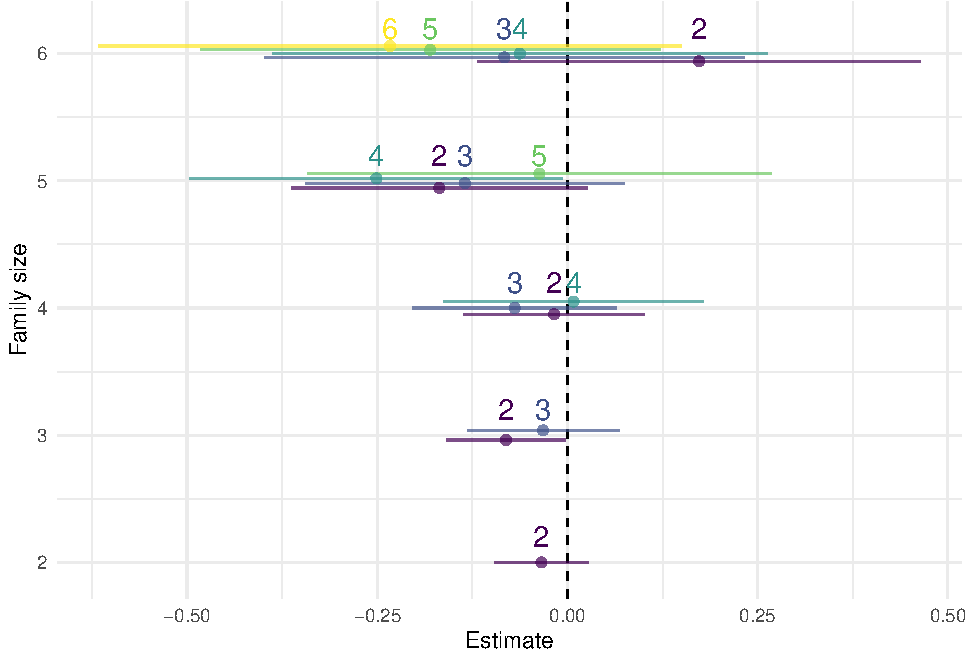
\includegraphics{trading-genetics_files/figure-latex/pic-bo-psea-interactions-1} 

}

\caption{Regressions of spouse PSEA: birth order dummies within different family sizes. Labels show birth order. Lines are 95 per cent confidence intervals. The omitted category is birth order 1.}\label{fig:pic-bo-psea-interactions}
\end{figure}

 
  \providecommand{\huxb}[2]{\arrayrulecolor[RGB]{#1}\global\arrayrulewidth=#2pt}
  \providecommand{\huxvb}[2]{\color[RGB]{#1}\vrule width #2pt}
  \providecommand{\huxtpad}[1]{\rule{0pt}{#1}}
  \providecommand{\huxbpad}[1]{\rule[-#1]{0pt}{#1}}

\begin{table}[ht]
\begin{centerbox}
\begin{threeparttable}
\captionsetup{justification=centering,singlelinecheck=off}
\caption{\label{tab:tbl-bo-psea-pgs} Regressions of spouse PSEA with controls for polygenic scores}
 \setlength{\tabcolsep}{0pt}
\begin{tabularx}{1\textwidth}{p{0.2\textwidth} p{0.2\textwidth} p{0.2\textwidth} p{0.2\textwidth} p{0.2\textwidth}}


\hhline{>{\huxb{0, 0, 0}{0.8}}->{\huxb{0, 0, 0}{0.8}}->{\huxb{0, 0, 0}{0.8}}->{\huxb{0, 0, 0}{0.8}}->{\huxb{0, 0, 0}{0.8}}-}
\arrayrulecolor{black}

\multicolumn{1}{!{\huxvb{0, 0, 0}{0}}p{0.2\textwidth}!{\huxvb{0, 0, 0}{0}}}{\hspace{6pt}\parbox[b]{0.2\textwidth-6pt-6pt}{\huxtpad{6pt + 1em}\centering \huxbpad{6pt}}} &
\multicolumn{1}{p{0.2\textwidth}!{\huxvb{0, 0, 0}{0}}}{\hspace{6pt}\parbox[b]{0.2\textwidth-6pt-6pt}{\huxtpad{6pt + 1em}\centering (1)\huxbpad{6pt}}} &
\multicolumn{1}{p{0.2\textwidth}!{\huxvb{0, 0, 0}{0}}}{\hspace{6pt}\parbox[b]{0.2\textwidth-6pt-6pt}{\huxtpad{6pt + 1em}\centering (2)\huxbpad{6pt}}} &
\multicolumn{1}{p{0.2\textwidth}!{\huxvb{0, 0, 0}{0}}}{\hspace{6pt}\parbox[b]{0.2\textwidth-6pt-6pt}{\huxtpad{6pt + 1em}\centering (3)\huxbpad{6pt}}} &
\multicolumn{1}{p{0.2\textwidth}!{\huxvb{0, 0, 0}{0}}}{\hspace{6pt}\parbox[b]{0.2\textwidth-6pt-6pt}{\huxtpad{6pt + 1em}\centering (4)\huxbpad{6pt}}} \tabularnewline[-0.5pt]


\hhline{>{\huxb{255, 255, 255}{0.4}}->{\huxb{0, 0, 0}{0.4}}->{\huxb{0, 0, 0}{0.4}}->{\huxb{0, 0, 0}{0.4}}->{\huxb{0, 0, 0}{0.4}}-}
\arrayrulecolor{black}

\multicolumn{1}{!{\huxvb{0, 0, 0}{0}}p{0.2\textwidth}!{\huxvb{0, 0, 0}{0}}}{\hspace{6pt}\parbox[b]{0.2\textwidth-6pt-6pt}{\huxtpad{6pt + 1em}\raggedright Birth order\huxbpad{6pt}}} &
\multicolumn{1}{p{0.2\textwidth}!{\huxvb{0, 0, 0}{0}}}{\hspace{6pt}\parbox[b]{0.2\textwidth-6pt-6pt}{\huxtpad{6pt + 1em}\raggedleft $-$0.0313\hphantom{0}\hphantom{0}\hphantom{0}\hphantom{0}\huxbpad{6pt}}} &
\multicolumn{1}{p{0.2\textwidth}!{\huxvb{0, 0, 0}{0}}}{\hspace{6pt}\parbox[b]{0.2\textwidth-6pt-6pt}{\huxtpad{6pt + 1em}\raggedleft $-$0.0047\hphantom{0}\hphantom{0}\hphantom{0}\hphantom{0}\huxbpad{6pt}}} &
\multicolumn{1}{p{0.2\textwidth}!{\huxvb{0, 0, 0}{0}}}{\hspace{6pt}\parbox[b]{0.2\textwidth-6pt-6pt}{\huxtpad{6pt + 1em}\raggedleft $-$0.0113\hphantom{0}\hphantom{0}\hphantom{0}\hphantom{0}\huxbpad{6pt}}} &
\multicolumn{1}{p{0.2\textwidth}!{\huxvb{0, 0, 0}{0}}}{\hspace{6pt}\parbox[b]{0.2\textwidth-6pt-6pt}{\huxtpad{6pt + 1em}\raggedleft $-$0.0049\hphantom{0}\hphantom{0}\hphantom{0}\hphantom{0}\huxbpad{6pt}}} \tabularnewline[-0.5pt]


\hhline{}
\arrayrulecolor{black}

\multicolumn{1}{!{\huxvb{0, 0, 0}{0}}p{0.2\textwidth}!{\huxvb{0, 0, 0}{0}}}{\hspace{6pt}\parbox[b]{0.2\textwidth-6pt-6pt}{\huxtpad{6pt + 1em}\raggedright \huxbpad{6pt}}} &
\multicolumn{1}{p{0.2\textwidth}!{\huxvb{0, 0, 0}{0}}}{\hspace{6pt}\parbox[b]{0.2\textwidth-6pt-6pt}{\huxtpad{6pt + 1em}\raggedleft (0.0183)\hphantom{0}\hphantom{0}\hphantom{0}\huxbpad{6pt}}} &
\multicolumn{1}{p{0.2\textwidth}!{\huxvb{0, 0, 0}{0}}}{\hspace{6pt}\parbox[b]{0.2\textwidth-6pt-6pt}{\huxtpad{6pt + 1em}\raggedleft (0.0177)\hphantom{0}\hphantom{0}\hphantom{0}\huxbpad{6pt}}} &
\multicolumn{1}{p{0.2\textwidth}!{\huxvb{0, 0, 0}{0}}}{\hspace{6pt}\parbox[b]{0.2\textwidth-6pt-6pt}{\huxtpad{6pt + 1em}\raggedleft (0.0311)\hphantom{0}\hphantom{0}\hphantom{0}\huxbpad{6pt}}} &
\multicolumn{1}{p{0.2\textwidth}!{\huxvb{0, 0, 0}{0}}}{\hspace{6pt}\parbox[b]{0.2\textwidth-6pt-6pt}{\huxtpad{6pt + 1em}\raggedleft (0.0308)\hphantom{0}\hphantom{0}\hphantom{0}\huxbpad{6pt}}} \tabularnewline[-0.5pt]


\hhline{}
\arrayrulecolor{black}

\multicolumn{1}{!{\huxvb{0, 0, 0}{0}}p{0.2\textwidth}!{\huxvb{0, 0, 0}{0}}}{\hspace{6pt}\parbox[b]{0.2\textwidth-6pt-6pt}{\huxtpad{6pt + 1em}\raggedright University\huxbpad{6pt}}} &
\multicolumn{1}{p{0.2\textwidth}!{\huxvb{0, 0, 0}{0}}}{\hspace{6pt}\parbox[b]{0.2\textwidth-6pt-6pt}{\huxtpad{6pt + 1em}\raggedleft \hphantom{0}\hphantom{0}\hphantom{0}\hphantom{0}\hphantom{0}\hphantom{0}\hphantom{0}\hphantom{0}\hphantom{0}\huxbpad{6pt}}} &
\multicolumn{1}{p{0.2\textwidth}!{\huxvb{0, 0, 0}{0}}}{\hspace{6pt}\parbox[b]{0.2\textwidth-6pt-6pt}{\huxtpad{6pt + 1em}\raggedleft 0.2178 ***\huxbpad{6pt}}} &
\multicolumn{1}{p{0.2\textwidth}!{\huxvb{0, 0, 0}{0}}}{\hspace{6pt}\parbox[b]{0.2\textwidth-6pt-6pt}{\huxtpad{6pt + 1em}\raggedleft \hphantom{0}\hphantom{0}\hphantom{0}\hphantom{0}\hphantom{0}\hphantom{0}\hphantom{0}\hphantom{0}\hphantom{0}\huxbpad{6pt}}} &
\multicolumn{1}{p{0.2\textwidth}!{\huxvb{0, 0, 0}{0}}}{\hspace{6pt}\parbox[b]{0.2\textwidth-6pt-6pt}{\huxtpad{6pt + 1em}\raggedleft 0.1534 ***\huxbpad{6pt}}} \tabularnewline[-0.5pt]


\hhline{}
\arrayrulecolor{black}

\multicolumn{1}{!{\huxvb{0, 0, 0}{0}}p{0.2\textwidth}!{\huxvb{0, 0, 0}{0}}}{\hspace{6pt}\parbox[b]{0.2\textwidth-6pt-6pt}{\huxtpad{6pt + 1em}\raggedright \huxbpad{6pt}}} &
\multicolumn{1}{p{0.2\textwidth}!{\huxvb{0, 0, 0}{0}}}{\hspace{6pt}\parbox[b]{0.2\textwidth-6pt-6pt}{\huxtpad{6pt + 1em}\raggedleft \hphantom{0}\hphantom{0}\hphantom{0}\hphantom{0}\hphantom{0}\hphantom{0}\hphantom{0}\hphantom{0}\hphantom{0}\huxbpad{6pt}}} &
\multicolumn{1}{p{0.2\textwidth}!{\huxvb{0, 0, 0}{0}}}{\hspace{6pt}\parbox[b]{0.2\textwidth-6pt-6pt}{\huxtpad{6pt + 1em}\raggedleft (0.0245)\hphantom{0}\hphantom{0}\hphantom{0}\huxbpad{6pt}}} &
\multicolumn{1}{p{0.2\textwidth}!{\huxvb{0, 0, 0}{0}}}{\hspace{6pt}\parbox[b]{0.2\textwidth-6pt-6pt}{\huxtpad{6pt + 1em}\raggedleft \hphantom{0}\hphantom{0}\hphantom{0}\hphantom{0}\hphantom{0}\hphantom{0}\hphantom{0}\hphantom{0}\hphantom{0}\huxbpad{6pt}}} &
\multicolumn{1}{p{0.2\textwidth}!{\huxvb{0, 0, 0}{0}}}{\hspace{6pt}\parbox[b]{0.2\textwidth-6pt-6pt}{\huxtpad{6pt + 1em}\raggedleft (0.0232)\hphantom{0}\hphantom{0}\hphantom{0}\huxbpad{6pt}}} \tabularnewline[-0.5pt]


\hhline{}
\arrayrulecolor{black}

\multicolumn{1}{!{\huxvb{0, 0, 0}{0}}p{0.2\textwidth}!{\huxvb{0, 0, 0}{0}}}{\hspace{6pt}\parbox[b]{0.2\textwidth-6pt-6pt}{\huxtpad{6pt + 1em}\raggedright Income\huxbpad{6pt}}} &
\multicolumn{1}{p{0.2\textwidth}!{\huxvb{0, 0, 0}{0}}}{\hspace{6pt}\parbox[b]{0.2\textwidth-6pt-6pt}{\huxtpad{6pt + 1em}\raggedleft \hphantom{0}\hphantom{0}\hphantom{0}\hphantom{0}\hphantom{0}\hphantom{0}\hphantom{0}\hphantom{0}\hphantom{0}\huxbpad{6pt}}} &
\multicolumn{1}{p{0.2\textwidth}!{\huxvb{0, 0, 0}{0}}}{\hspace{6pt}\parbox[b]{0.2\textwidth-6pt-6pt}{\huxtpad{6pt + 1em}\raggedleft \hphantom{0}\hphantom{0}\hphantom{0}\hphantom{0}\hphantom{0}\hphantom{0}\hphantom{0}\hphantom{0}\hphantom{0}\huxbpad{6pt}}} &
\multicolumn{1}{p{0.2\textwidth}!{\huxvb{0, 0, 0}{0}}}{\hspace{6pt}\parbox[b]{0.2\textwidth-6pt-6pt}{\huxtpad{6pt + 1em}\raggedleft 0.0037 ***\huxbpad{6pt}}} &
\multicolumn{1}{p{0.2\textwidth}!{\huxvb{0, 0, 0}{0}}}{\hspace{6pt}\parbox[b]{0.2\textwidth-6pt-6pt}{\huxtpad{6pt + 1em}\raggedleft 0.0030 ***\huxbpad{6pt}}} \tabularnewline[-0.5pt]


\hhline{}
\arrayrulecolor{black}

\multicolumn{1}{!{\huxvb{0, 0, 0}{0}}p{0.2\textwidth}!{\huxvb{0, 0, 0}{0}}}{\hspace{6pt}\parbox[b]{0.2\textwidth-6pt-6pt}{\huxtpad{6pt + 1em}\raggedright \huxbpad{6pt}}} &
\multicolumn{1}{p{0.2\textwidth}!{\huxvb{0, 0, 0}{0}}}{\hspace{6pt}\parbox[b]{0.2\textwidth-6pt-6pt}{\huxtpad{6pt + 1em}\raggedleft \hphantom{0}\hphantom{0}\hphantom{0}\hphantom{0}\hphantom{0}\hphantom{0}\hphantom{0}\hphantom{0}\hphantom{0}\huxbpad{6pt}}} &
\multicolumn{1}{p{0.2\textwidth}!{\huxvb{0, 0, 0}{0}}}{\hspace{6pt}\parbox[b]{0.2\textwidth-6pt-6pt}{\huxtpad{6pt + 1em}\raggedleft \hphantom{0}\hphantom{0}\hphantom{0}\hphantom{0}\hphantom{0}\hphantom{0}\hphantom{0}\hphantom{0}\hphantom{0}\huxbpad{6pt}}} &
\multicolumn{1}{p{0.2\textwidth}!{\huxvb{0, 0, 0}{0}}}{\hspace{6pt}\parbox[b]{0.2\textwidth-6pt-6pt}{\huxtpad{6pt + 1em}\raggedleft (0.0007)\hphantom{0}\hphantom{0}\hphantom{0}\huxbpad{6pt}}} &
\multicolumn{1}{p{0.2\textwidth}!{\huxvb{0, 0, 0}{0}}}{\hspace{6pt}\parbox[b]{0.2\textwidth-6pt-6pt}{\huxtpad{6pt + 1em}\raggedleft (0.0007)\hphantom{0}\hphantom{0}\hphantom{0}\huxbpad{6pt}}} \tabularnewline[-0.5pt]


\hhline{}
\arrayrulecolor{black}

\multicolumn{1}{!{\huxvb{0, 0, 0}{0}}p{0.2\textwidth}!{\huxvb{0, 0, 0}{0}}}{\hspace{6pt}\parbox[b]{0.2\textwidth-6pt-6pt}{\huxtpad{6pt + 1em}\raggedright Fluid IQ\huxbpad{6pt}}} &
\multicolumn{1}{p{0.2\textwidth}!{\huxvb{0, 0, 0}{0}}}{\hspace{6pt}\parbox[b]{0.2\textwidth-6pt-6pt}{\huxtpad{6pt + 1em}\raggedleft \hphantom{0}\hphantom{0}\hphantom{0}\hphantom{0}\hphantom{0}\hphantom{0}\hphantom{0}\hphantom{0}\hphantom{0}\huxbpad{6pt}}} &
\multicolumn{1}{p{0.2\textwidth}!{\huxvb{0, 0, 0}{0}}}{\hspace{6pt}\parbox[b]{0.2\textwidth-6pt-6pt}{\huxtpad{6pt + 1em}\raggedleft 0.0168 *\hphantom{0}\hphantom{0}\huxbpad{6pt}}} &
\multicolumn{1}{p{0.2\textwidth}!{\huxvb{0, 0, 0}{0}}}{\hspace{6pt}\parbox[b]{0.2\textwidth-6pt-6pt}{\huxtpad{6pt + 1em}\raggedleft 0.0198\hphantom{0}\hphantom{0}\hphantom{0}\hphantom{0}\huxbpad{6pt}}} &
\multicolumn{1}{p{0.2\textwidth}!{\huxvb{0, 0, 0}{0}}}{\hspace{6pt}\parbox[b]{0.2\textwidth-6pt-6pt}{\huxtpad{6pt + 1em}\raggedleft 0.0110\hphantom{0}\hphantom{0}\hphantom{0}\hphantom{0}\huxbpad{6pt}}} \tabularnewline[-0.5pt]


\hhline{}
\arrayrulecolor{black}

\multicolumn{1}{!{\huxvb{0, 0, 0}{0}}p{0.2\textwidth}!{\huxvb{0, 0, 0}{0}}}{\hspace{6pt}\parbox[b]{0.2\textwidth-6pt-6pt}{\huxtpad{6pt + 1em}\raggedright \huxbpad{6pt}}} &
\multicolumn{1}{p{0.2\textwidth}!{\huxvb{0, 0, 0}{0}}}{\hspace{6pt}\parbox[b]{0.2\textwidth-6pt-6pt}{\huxtpad{6pt + 1em}\raggedleft \hphantom{0}\hphantom{0}\hphantom{0}\hphantom{0}\hphantom{0}\hphantom{0}\hphantom{0}\hphantom{0}\hphantom{0}\huxbpad{6pt}}} &
\multicolumn{1}{p{0.2\textwidth}!{\huxvb{0, 0, 0}{0}}}{\hspace{6pt}\parbox[b]{0.2\textwidth-6pt-6pt}{\huxtpad{6pt + 1em}\raggedleft (0.0066)\hphantom{0}\hphantom{0}\hphantom{0}\huxbpad{6pt}}} &
\multicolumn{1}{p{0.2\textwidth}!{\huxvb{0, 0, 0}{0}}}{\hspace{6pt}\parbox[b]{0.2\textwidth-6pt-6pt}{\huxtpad{6pt + 1em}\raggedleft (0.0116)\hphantom{0}\hphantom{0}\hphantom{0}\huxbpad{6pt}}} &
\multicolumn{1}{p{0.2\textwidth}!{\huxvb{0, 0, 0}{0}}}{\hspace{6pt}\parbox[b]{0.2\textwidth-6pt-6pt}{\huxtpad{6pt + 1em}\raggedleft (0.0120)\hphantom{0}\hphantom{0}\hphantom{0}\huxbpad{6pt}}} \tabularnewline[-0.5pt]


\hhline{}
\arrayrulecolor{black}

\multicolumn{1}{!{\huxvb{0, 0, 0}{0}}p{0.2\textwidth}!{\huxvb{0, 0, 0}{0}}}{\hspace{6pt}\parbox[b]{0.2\textwidth-6pt-6pt}{\huxtpad{6pt + 1em}\raggedright Height\huxbpad{6pt}}} &
\multicolumn{1}{p{0.2\textwidth}!{\huxvb{0, 0, 0}{0}}}{\hspace{6pt}\parbox[b]{0.2\textwidth-6pt-6pt}{\huxtpad{6pt + 1em}\raggedleft \hphantom{0}\hphantom{0}\hphantom{0}\hphantom{0}\hphantom{0}\hphantom{0}\hphantom{0}\hphantom{0}\hphantom{0}\huxbpad{6pt}}} &
\multicolumn{1}{p{0.2\textwidth}!{\huxvb{0, 0, 0}{0}}}{\hspace{6pt}\parbox[b]{0.2\textwidth-6pt-6pt}{\huxtpad{6pt + 1em}\raggedleft 0.0029 *\hphantom{0}\hphantom{0}\huxbpad{6pt}}} &
\multicolumn{1}{p{0.2\textwidth}!{\huxvb{0, 0, 0}{0}}}{\hspace{6pt}\parbox[b]{0.2\textwidth-6pt-6pt}{\huxtpad{6pt + 1em}\raggedleft 0.0046 *\hphantom{0}\hphantom{0}\huxbpad{6pt}}} &
\multicolumn{1}{p{0.2\textwidth}!{\huxvb{0, 0, 0}{0}}}{\hspace{6pt}\parbox[b]{0.2\textwidth-6pt-6pt}{\huxtpad{6pt + 1em}\raggedleft 0.0042 *\hphantom{0}\hphantom{0}\huxbpad{6pt}}} \tabularnewline[-0.5pt]


\hhline{}
\arrayrulecolor{black}

\multicolumn{1}{!{\huxvb{0, 0, 0}{0}}p{0.2\textwidth}!{\huxvb{0, 0, 0}{0}}}{\hspace{6pt}\parbox[b]{0.2\textwidth-6pt-6pt}{\huxtpad{6pt + 1em}\raggedright \huxbpad{6pt}}} &
\multicolumn{1}{p{0.2\textwidth}!{\huxvb{0, 0, 0}{0}}}{\hspace{6pt}\parbox[b]{0.2\textwidth-6pt-6pt}{\huxtpad{6pt + 1em}\raggedleft \hphantom{0}\hphantom{0}\hphantom{0}\hphantom{0}\hphantom{0}\hphantom{0}\hphantom{0}\hphantom{0}\hphantom{0}\huxbpad{6pt}}} &
\multicolumn{1}{p{0.2\textwidth}!{\huxvb{0, 0, 0}{0}}}{\hspace{6pt}\parbox[b]{0.2\textwidth-6pt-6pt}{\huxtpad{6pt + 1em}\raggedleft (0.0011)\hphantom{0}\hphantom{0}\hphantom{0}\huxbpad{6pt}}} &
\multicolumn{1}{p{0.2\textwidth}!{\huxvb{0, 0, 0}{0}}}{\hspace{6pt}\parbox[b]{0.2\textwidth-6pt-6pt}{\huxtpad{6pt + 1em}\raggedleft (0.0018)\hphantom{0}\hphantom{0}\hphantom{0}\huxbpad{6pt}}} &
\multicolumn{1}{p{0.2\textwidth}!{\huxvb{0, 0, 0}{0}}}{\hspace{6pt}\parbox[b]{0.2\textwidth-6pt-6pt}{\huxtpad{6pt + 1em}\raggedleft (0.0018)\hphantom{0}\hphantom{0}\hphantom{0}\huxbpad{6pt}}} \tabularnewline[-0.5pt]


\hhline{}
\arrayrulecolor{black}

\multicolumn{1}{!{\huxvb{0, 0, 0}{0}}p{0.2\textwidth}!{\huxvb{0, 0, 0}{0}}}{\hspace{6pt}\parbox[b]{0.2\textwidth-6pt-6pt}{\huxtpad{6pt + 1em}\raggedright BMI\huxbpad{6pt}}} &
\multicolumn{1}{p{0.2\textwidth}!{\huxvb{0, 0, 0}{0}}}{\hspace{6pt}\parbox[b]{0.2\textwidth-6pt-6pt}{\huxtpad{6pt + 1em}\raggedleft \hphantom{0}\hphantom{0}\hphantom{0}\hphantom{0}\hphantom{0}\hphantom{0}\hphantom{0}\hphantom{0}\hphantom{0}\huxbpad{6pt}}} &
\multicolumn{1}{p{0.2\textwidth}!{\huxvb{0, 0, 0}{0}}}{\hspace{6pt}\parbox[b]{0.2\textwidth-6pt-6pt}{\huxtpad{6pt + 1em}\raggedleft $-$0.0109 ***\huxbpad{6pt}}} &
\multicolumn{1}{p{0.2\textwidth}!{\huxvb{0, 0, 0}{0}}}{\hspace{6pt}\parbox[b]{0.2\textwidth-6pt-6pt}{\huxtpad{6pt + 1em}\raggedleft $-$0.0112 **\hphantom{0}\huxbpad{6pt}}} &
\multicolumn{1}{p{0.2\textwidth}!{\huxvb{0, 0, 0}{0}}}{\hspace{6pt}\parbox[b]{0.2\textwidth-6pt-6pt}{\huxtpad{6pt + 1em}\raggedleft $-$0.0107 *\hphantom{0}\hphantom{0}\huxbpad{6pt}}} \tabularnewline[-0.5pt]


\hhline{}
\arrayrulecolor{black}

\multicolumn{1}{!{\huxvb{0, 0, 0}{0}}p{0.2\textwidth}!{\huxvb{0, 0, 0}{0}}}{\hspace{6pt}\parbox[b]{0.2\textwidth-6pt-6pt}{\huxtpad{6pt + 1em}\raggedright \huxbpad{6pt}}} &
\multicolumn{1}{p{0.2\textwidth}!{\huxvb{0, 0, 0}{0}}}{\hspace{6pt}\parbox[b]{0.2\textwidth-6pt-6pt}{\huxtpad{6pt + 1em}\raggedleft \hphantom{0}\hphantom{0}\hphantom{0}\hphantom{0}\hphantom{0}\hphantom{0}\hphantom{0}\hphantom{0}\hphantom{0}\huxbpad{6pt}}} &
\multicolumn{1}{p{0.2\textwidth}!{\huxvb{0, 0, 0}{0}}}{\hspace{6pt}\parbox[b]{0.2\textwidth-6pt-6pt}{\huxtpad{6pt + 1em}\raggedleft (0.0023)\hphantom{0}\hphantom{0}\hphantom{0}\huxbpad{6pt}}} &
\multicolumn{1}{p{0.2\textwidth}!{\huxvb{0, 0, 0}{0}}}{\hspace{6pt}\parbox[b]{0.2\textwidth-6pt-6pt}{\huxtpad{6pt + 1em}\raggedleft (0.0039)\hphantom{0}\hphantom{0}\hphantom{0}\huxbpad{6pt}}} &
\multicolumn{1}{p{0.2\textwidth}!{\huxvb{0, 0, 0}{0}}}{\hspace{6pt}\parbox[b]{0.2\textwidth-6pt-6pt}{\huxtpad{6pt + 1em}\raggedleft (0.0039)\hphantom{0}\hphantom{0}\hphantom{0}\huxbpad{6pt}}} \tabularnewline[-0.5pt]


\hhline{}
\arrayrulecolor{black}

\multicolumn{1}{!{\huxvb{0, 0, 0}{0}}p{0.2\textwidth}!{\huxvb{0, 0, 0}{0}}}{\hspace{6pt}\parbox[b]{0.2\textwidth-6pt-6pt}{\huxtpad{6pt + 1em}\raggedright Self-reported health\huxbpad{6pt}}} &
\multicolumn{1}{p{0.2\textwidth}!{\huxvb{0, 0, 0}{0}}}{\hspace{6pt}\parbox[b]{0.2\textwidth-6pt-6pt}{\huxtpad{6pt + 1em}\raggedleft \hphantom{0}\hphantom{0}\hphantom{0}\hphantom{0}\hphantom{0}\hphantom{0}\hphantom{0}\hphantom{0}\hphantom{0}\huxbpad{6pt}}} &
\multicolumn{1}{p{0.2\textwidth}!{\huxvb{0, 0, 0}{0}}}{\hspace{6pt}\parbox[b]{0.2\textwidth-6pt-6pt}{\huxtpad{6pt + 1em}\raggedleft 0.0173\hphantom{0}\hphantom{0}\hphantom{0}\hphantom{0}\huxbpad{6pt}}} &
\multicolumn{1}{p{0.2\textwidth}!{\huxvb{0, 0, 0}{0}}}{\hspace{6pt}\parbox[b]{0.2\textwidth-6pt-6pt}{\huxtpad{6pt + 1em}\raggedleft 0.0138\hphantom{0}\hphantom{0}\hphantom{0}\hphantom{0}\huxbpad{6pt}}} &
\multicolumn{1}{p{0.2\textwidth}!{\huxvb{0, 0, 0}{0}}}{\hspace{6pt}\parbox[b]{0.2\textwidth-6pt-6pt}{\huxtpad{6pt + 1em}\raggedleft 0.0071\hphantom{0}\hphantom{0}\hphantom{0}\hphantom{0}\huxbpad{6pt}}} \tabularnewline[-0.5pt]


\hhline{}
\arrayrulecolor{black}

\multicolumn{1}{!{\huxvb{0, 0, 0}{0}}p{0.2\textwidth}!{\huxvb{0, 0, 0}{0}}}{\hspace{6pt}\parbox[b]{0.2\textwidth-6pt-6pt}{\huxtpad{6pt + 1em}\raggedright \huxbpad{6pt}}} &
\multicolumn{1}{p{0.2\textwidth}!{\huxvb{0, 0, 0}{0}}}{\hspace{6pt}\parbox[b]{0.2\textwidth-6pt-6pt}{\huxtpad{6pt + 1em}\raggedleft \hphantom{0}\hphantom{0}\hphantom{0}\hphantom{0}\hphantom{0}\hphantom{0}\hphantom{0}\hphantom{0}\hphantom{0}\huxbpad{6pt}}} &
\multicolumn{1}{p{0.2\textwidth}!{\huxvb{0, 0, 0}{0}}}{\hspace{6pt}\parbox[b]{0.2\textwidth-6pt-6pt}{\huxtpad{6pt + 1em}\raggedleft (0.0199)\hphantom{0}\hphantom{0}\hphantom{0}\huxbpad{6pt}}} &
\multicolumn{1}{p{0.2\textwidth}!{\huxvb{0, 0, 0}{0}}}{\hspace{6pt}\parbox[b]{0.2\textwidth-6pt-6pt}{\huxtpad{6pt + 1em}\raggedleft (0.0341)\hphantom{0}\hphantom{0}\hphantom{0}\huxbpad{6pt}}} &
\multicolumn{1}{p{0.2\textwidth}!{\huxvb{0, 0, 0}{0}}}{\hspace{6pt}\parbox[b]{0.2\textwidth-6pt-6pt}{\huxtpad{6pt + 1em}\raggedleft (0.0339)\hphantom{0}\hphantom{0}\hphantom{0}\huxbpad{6pt}}} \tabularnewline[-0.5pt]


\hhline{}
\arrayrulecolor{black}

\multicolumn{1}{!{\huxvb{0, 0, 0}{0}}p{0.2\textwidth}!{\huxvb{0, 0, 0}{0}}}{\hspace{6pt}\parbox[b]{0.2\textwidth-6pt-6pt}{\huxtpad{6pt + 1em}\raggedright Own PSEA\huxbpad{6pt}}} &
\multicolumn{1}{p{0.2\textwidth}!{\huxvb{0, 0, 0}{0}}}{\hspace{6pt}\parbox[b]{0.2\textwidth-6pt-6pt}{\huxtpad{6pt + 1em}\raggedleft 0.0519 ***\huxbpad{6pt}}} &
\multicolumn{1}{p{0.2\textwidth}!{\huxvb{0, 0, 0}{0}}}{\hspace{6pt}\parbox[b]{0.2\textwidth-6pt-6pt}{\huxtpad{6pt + 1em}\raggedleft 0.0231 +\hphantom{0}\hphantom{0}\huxbpad{6pt}}} &
\multicolumn{1}{p{0.2\textwidth}!{\huxvb{0, 0, 0}{0}}}{\hspace{6pt}\parbox[b]{0.2\textwidth-6pt-6pt}{\huxtpad{6pt + 1em}\raggedleft 0.0178\hphantom{0}\hphantom{0}\hphantom{0}\hphantom{0}\huxbpad{6pt}}} &
\multicolumn{1}{p{0.2\textwidth}!{\huxvb{0, 0, 0}{0}}}{\hspace{6pt}\parbox[b]{0.2\textwidth-6pt-6pt}{\huxtpad{6pt + 1em}\raggedleft 0.0084\hphantom{0}\hphantom{0}\hphantom{0}\hphantom{0}\huxbpad{6pt}}} \tabularnewline[-0.5pt]


\hhline{}
\arrayrulecolor{black}

\multicolumn{1}{!{\huxvb{0, 0, 0}{0}}p{0.2\textwidth}!{\huxvb{0, 0, 0}{0}}}{\hspace{6pt}\parbox[b]{0.2\textwidth-6pt-6pt}{\huxtpad{6pt + 1em}\raggedright \huxbpad{6pt}}} &
\multicolumn{1}{p{0.2\textwidth}!{\huxvb{0, 0, 0}{0}}}{\hspace{6pt}\parbox[b]{0.2\textwidth-6pt-6pt}{\huxtpad{6pt + 1em}\raggedleft (0.0111)\hphantom{0}\hphantom{0}\hphantom{0}\huxbpad{6pt}}} &
\multicolumn{1}{p{0.2\textwidth}!{\huxvb{0, 0, 0}{0}}}{\hspace{6pt}\parbox[b]{0.2\textwidth-6pt-6pt}{\huxtpad{6pt + 1em}\raggedleft (0.0115)\hphantom{0}\hphantom{0}\hphantom{0}\huxbpad{6pt}}} &
\multicolumn{1}{p{0.2\textwidth}!{\huxvb{0, 0, 0}{0}}}{\hspace{6pt}\parbox[b]{0.2\textwidth-6pt-6pt}{\huxtpad{6pt + 1em}\raggedleft (0.0245)\hphantom{0}\hphantom{0}\hphantom{0}\huxbpad{6pt}}} &
\multicolumn{1}{p{0.2\textwidth}!{\huxvb{0, 0, 0}{0}}}{\hspace{6pt}\parbox[b]{0.2\textwidth-6pt-6pt}{\huxtpad{6pt + 1em}\raggedleft (0.0243)\hphantom{0}\hphantom{0}\hphantom{0}\huxbpad{6pt}}} \tabularnewline[-0.5pt]


\hhline{}
\arrayrulecolor{black}

\multicolumn{1}{!{\huxvb{0, 0, 0}{0}}p{0.2\textwidth}!{\huxvb{0, 0, 0}{0}}}{\hspace{6pt}\parbox[b]{0.2\textwidth-6pt-6pt}{\huxtpad{6pt + 1em}\raggedright Parents' age at birth\huxbpad{6pt}}} &
\multicolumn{1}{p{0.2\textwidth}!{\huxvb{0, 0, 0}{0}}}{\hspace{6pt}\parbox[b]{0.2\textwidth-6pt-6pt}{\huxtpad{6pt + 1em}\raggedleft 0.0114 ***\huxbpad{6pt}}} &
\multicolumn{1}{p{0.2\textwidth}!{\huxvb{0, 0, 0}{0}}}{\hspace{6pt}\parbox[b]{0.2\textwidth-6pt-6pt}{\huxtpad{6pt + 1em}\raggedleft 0.0052 +\hphantom{0}\hphantom{0}\huxbpad{6pt}}} &
\multicolumn{1}{p{0.2\textwidth}!{\huxvb{0, 0, 0}{0}}}{\hspace{6pt}\parbox[b]{0.2\textwidth-6pt-6pt}{\huxtpad{6pt + 1em}\raggedleft 0.0093 *\hphantom{0}\hphantom{0}\huxbpad{6pt}}} &
\multicolumn{1}{p{0.2\textwidth}!{\huxvb{0, 0, 0}{0}}}{\hspace{6pt}\parbox[b]{0.2\textwidth-6pt-6pt}{\huxtpad{6pt + 1em}\raggedleft 0.0080 +\hphantom{0}\hphantom{0}\huxbpad{6pt}}} \tabularnewline[-0.5pt]


\hhline{}
\arrayrulecolor{black}

\multicolumn{1}{!{\huxvb{0, 0, 0}{0}}p{0.2\textwidth}!{\huxvb{0, 0, 0}{0}}}{\hspace{6pt}\parbox[b]{0.2\textwidth-6pt-6pt}{\huxtpad{6pt + 1em}\raggedright \huxbpad{6pt}}} &
\multicolumn{1}{p{0.2\textwidth}!{\huxvb{0, 0, 0}{0}}}{\hspace{6pt}\parbox[b]{0.2\textwidth-6pt-6pt}{\huxtpad{6pt + 1em}\raggedleft (0.0028)\hphantom{0}\hphantom{0}\hphantom{0}\huxbpad{6pt}}} &
\multicolumn{1}{p{0.2\textwidth}!{\huxvb{0, 0, 0}{0}}}{\hspace{6pt}\parbox[b]{0.2\textwidth-6pt-6pt}{\huxtpad{6pt + 1em}\raggedleft (0.0028)\hphantom{0}\hphantom{0}\hphantom{0}\huxbpad{6pt}}} &
\multicolumn{1}{p{0.2\textwidth}!{\huxvb{0, 0, 0}{0}}}{\hspace{6pt}\parbox[b]{0.2\textwidth-6pt-6pt}{\huxtpad{6pt + 1em}\raggedleft (0.0040)\hphantom{0}\hphantom{0}\hphantom{0}\huxbpad{6pt}}} &
\multicolumn{1}{p{0.2\textwidth}!{\huxvb{0, 0, 0}{0}}}{\hspace{6pt}\parbox[b]{0.2\textwidth-6pt-6pt}{\huxtpad{6pt + 1em}\raggedleft (0.0041)\hphantom{0}\hphantom{0}\hphantom{0}\huxbpad{6pt}}} \tabularnewline[-0.5pt]


\hhline{>{\huxb{255, 255, 255}{0.4}}->{\huxb{0, 0, 0}{0.4}}->{\huxb{0, 0, 0}{0.4}}->{\huxb{0, 0, 0}{0.4}}->{\huxb{0, 0, 0}{0.4}}-}
\arrayrulecolor{black}

\multicolumn{1}{!{\huxvb{0, 0, 0}{0}}p{0.2\textwidth}!{\huxvb{0, 0, 0}{0}}}{\hspace{6pt}\parbox[b]{0.2\textwidth-6pt-6pt}{\huxtpad{6pt + 1em}\raggedright Family size dummies\huxbpad{6pt}}} &
\multicolumn{1}{p{0.2\textwidth}!{\huxvb{0, 0, 0}{0}}}{\hspace{6pt}\parbox[b]{0.2\textwidth-6pt-6pt}{\huxtpad{6pt + 1em}\centering Yes\huxbpad{6pt}}} &
\multicolumn{1}{p{0.2\textwidth}!{\huxvb{0, 0, 0}{0}}}{\hspace{6pt}\parbox[b]{0.2\textwidth-6pt-6pt}{\huxtpad{6pt + 1em}\centering Yes\huxbpad{6pt}}} &
\multicolumn{1}{p{0.2\textwidth}!{\huxvb{0, 0, 0}{0}}}{\hspace{6pt}\parbox[b]{0.2\textwidth-6pt-6pt}{\huxtpad{6pt + 1em}\centering Yes\huxbpad{6pt}}} &
\multicolumn{1}{p{0.2\textwidth}!{\huxvb{0, 0, 0}{0}}}{\hspace{6pt}\parbox[b]{0.2\textwidth-6pt-6pt}{\huxtpad{6pt + 1em}\centering Yes\huxbpad{6pt}}} \tabularnewline[-0.5pt]


\hhline{}
\arrayrulecolor{black}

\multicolumn{1}{!{\huxvb{0, 0, 0}{0}}p{0.2\textwidth}!{\huxvb{0, 0, 0}{0}}}{\hspace{6pt}\parbox[b]{0.2\textwidth-6pt-6pt}{\huxtpad{6pt + 1em}\raggedright Birth month dummies\huxbpad{6pt}}} &
\multicolumn{1}{p{0.2\textwidth}!{\huxvb{0, 0, 0}{0}}}{\hspace{6pt}\parbox[b]{0.2\textwidth-6pt-6pt}{\huxtpad{6pt + 1em}\centering Yes\huxbpad{6pt}}} &
\multicolumn{1}{p{0.2\textwidth}!{\huxvb{0, 0, 0}{0}}}{\hspace{6pt}\parbox[b]{0.2\textwidth-6pt-6pt}{\huxtpad{6pt + 1em}\centering Yes\huxbpad{6pt}}} &
\multicolumn{1}{p{0.2\textwidth}!{\huxvb{0, 0, 0}{0}}}{\hspace{6pt}\parbox[b]{0.2\textwidth-6pt-6pt}{\huxtpad{6pt + 1em}\centering Yes\huxbpad{6pt}}} &
\multicolumn{1}{p{0.2\textwidth}!{\huxvb{0, 0, 0}{0}}}{\hspace{6pt}\parbox[b]{0.2\textwidth-6pt-6pt}{\huxtpad{6pt + 1em}\centering Yes\huxbpad{6pt}}} \tabularnewline[-0.5pt]


\hhline{}
\arrayrulecolor{black}

\multicolumn{1}{!{\huxvb{0, 0, 0}{0}}p{0.2\textwidth}!{\huxvb{0, 0, 0}{0}}}{\hspace{6pt}\parbox[b]{0.2\textwidth-6pt-6pt}{\huxtpad{6pt + 1em}\raggedright Birth year dummies\huxbpad{6pt}}} &
\multicolumn{1}{p{0.2\textwidth}!{\huxvb{0, 0, 0}{0}}}{\hspace{6pt}\parbox[b]{0.2\textwidth-6pt-6pt}{\huxtpad{6pt + 1em}\centering Yes\huxbpad{6pt}}} &
\multicolumn{1}{p{0.2\textwidth}!{\huxvb{0, 0, 0}{0}}}{\hspace{6pt}\parbox[b]{0.2\textwidth-6pt-6pt}{\huxtpad{6pt + 1em}\centering Yes\huxbpad{6pt}}} &
\multicolumn{1}{p{0.2\textwidth}!{\huxvb{0, 0, 0}{0}}}{\hspace{6pt}\parbox[b]{0.2\textwidth-6pt-6pt}{\huxtpad{6pt + 1em}\centering Yes\huxbpad{6pt}}} &
\multicolumn{1}{p{0.2\textwidth}!{\huxvb{0, 0, 0}{0}}}{\hspace{6pt}\parbox[b]{0.2\textwidth-6pt-6pt}{\huxtpad{6pt + 1em}\centering Yes\huxbpad{6pt}}} \tabularnewline[-0.5pt]


\hhline{}
\arrayrulecolor{black}

\multicolumn{1}{!{\huxvb{0, 0, 0}{0}}p{0.2\textwidth}!{\huxvb{0, 0, 0}{0}}}{\hspace{6pt}\parbox[b]{0.2\textwidth-6pt-6pt}{\huxtpad{6pt + 1em}\raggedright Polygenic score controls\huxbpad{6pt}}} &
\multicolumn{1}{p{0.2\textwidth}!{\huxvb{0, 0, 0}{0}}}{\hspace{6pt}\parbox[b]{0.2\textwidth-6pt-6pt}{\huxtpad{6pt + 1em}\centering Yes\huxbpad{6pt}}} &
\multicolumn{1}{p{0.2\textwidth}!{\huxvb{0, 0, 0}{0}}}{\hspace{6pt}\parbox[b]{0.2\textwidth-6pt-6pt}{\huxtpad{6pt + 1em}\centering Yes\huxbpad{6pt}}} &
\multicolumn{1}{p{0.2\textwidth}!{\huxvb{0, 0, 0}{0}}}{\hspace{6pt}\parbox[b]{0.2\textwidth-6pt-6pt}{\huxtpad{6pt + 1em}\centering Yes\huxbpad{6pt}}} &
\multicolumn{1}{p{0.2\textwidth}!{\huxvb{0, 0, 0}{0}}}{\hspace{6pt}\parbox[b]{0.2\textwidth-6pt-6pt}{\huxtpad{6pt + 1em}\centering Yes\huxbpad{6pt}}} \tabularnewline[-0.5pt]


\hhline{>{\huxb{255, 255, 255}{0.4}}->{\huxb{0, 0, 0}{0.4}}->{\huxb{0, 0, 0}{0.4}}->{\huxb{0, 0, 0}{0.4}}->{\huxb{0, 0, 0}{0.4}}-}
\arrayrulecolor{black}

\multicolumn{1}{!{\huxvb{0, 0, 0}{0}}p{0.2\textwidth}!{\huxvb{0, 0, 0}{0}}}{\hspace{6pt}\parbox[b]{0.2\textwidth-6pt-6pt}{\huxtpad{6pt + 1em}\raggedright N\huxbpad{6pt}}} &
\multicolumn{1}{p{0.2\textwidth}!{\huxvb{0, 0, 0}{0}}}{\hspace{6pt}\parbox[b]{0.2\textwidth-6pt-6pt}{\huxtpad{6pt + 1em}\raggedleft 10206\hphantom{0}\hphantom{0}\hphantom{0}\hphantom{0}\hphantom{0}\hphantom{0}\hphantom{0}\hphantom{0}\hphantom{0}\huxbpad{6pt}}} &
\multicolumn{1}{p{0.2\textwidth}!{\huxvb{0, 0, 0}{0}}}{\hspace{6pt}\parbox[b]{0.2\textwidth-6pt-6pt}{\huxtpad{6pt + 1em}\raggedleft 10206\hphantom{0}\hphantom{0}\hphantom{0}\hphantom{0}\hphantom{0}\hphantom{0}\hphantom{0}\hphantom{0}\hphantom{0}\huxbpad{6pt}}} &
\multicolumn{1}{p{0.2\textwidth}!{\huxvb{0, 0, 0}{0}}}{\hspace{6pt}\parbox[b]{0.2\textwidth-6pt-6pt}{\huxtpad{6pt + 1em}\raggedleft 3407\hphantom{0}\hphantom{0}\hphantom{0}\hphantom{0}\hphantom{0}\hphantom{0}\hphantom{0}\hphantom{0}\hphantom{0}\huxbpad{6pt}}} &
\multicolumn{1}{p{0.2\textwidth}!{\huxvb{0, 0, 0}{0}}}{\hspace{6pt}\parbox[b]{0.2\textwidth-6pt-6pt}{\huxtpad{6pt + 1em}\raggedleft 3407\hphantom{0}\hphantom{0}\hphantom{0}\hphantom{0}\hphantom{0}\hphantom{0}\hphantom{0}\hphantom{0}\hphantom{0}\huxbpad{6pt}}} \tabularnewline[-0.5pt]


\hhline{}
\arrayrulecolor{black}

\multicolumn{1}{!{\huxvb{0, 0, 0}{0}}p{0.2\textwidth}!{\huxvb{0, 0, 0}{0}}}{\hspace{6pt}\parbox[b]{0.2\textwidth-6pt-6pt}{\huxtpad{6pt + 1em}\raggedright R2\huxbpad{6pt}}} &
\multicolumn{1}{p{0.2\textwidth}!{\huxvb{0, 0, 0}{0}}}{\hspace{6pt}\parbox[b]{0.2\textwidth-6pt-6pt}{\huxtpad{6pt + 1em}\raggedleft 0.013\hphantom{0}\hphantom{0}\hphantom{0}\hphantom{0}\hphantom{0}\huxbpad{6pt}}} &
\multicolumn{1}{p{0.2\textwidth}!{\huxvb{0, 0, 0}{0}}}{\hspace{6pt}\parbox[b]{0.2\textwidth-6pt-6pt}{\huxtpad{6pt + 1em}\raggedleft 0.032\hphantom{0}\hphantom{0}\hphantom{0}\hphantom{0}\hphantom{0}\huxbpad{6pt}}} &
\multicolumn{1}{p{0.2\textwidth}!{\huxvb{0, 0, 0}{0}}}{\hspace{6pt}\parbox[b]{0.2\textwidth-6pt-6pt}{\huxtpad{6pt + 1em}\raggedleft 0.030\hphantom{0}\hphantom{0}\hphantom{0}\hphantom{0}\hphantom{0}\huxbpad{6pt}}} &
\multicolumn{1}{p{0.2\textwidth}!{\huxvb{0, 0, 0}{0}}}{\hspace{6pt}\parbox[b]{0.2\textwidth-6pt-6pt}{\huxtpad{6pt + 1em}\raggedleft 0.035\hphantom{0}\hphantom{0}\hphantom{0}\hphantom{0}\hphantom{0}\huxbpad{6pt}}} \tabularnewline[-0.5pt]


\hhline{>{\huxb{0, 0, 0}{0.8}}->{\huxb{0, 0, 0}{0.8}}->{\huxb{0, 0, 0}{0.8}}->{\huxb{0, 0, 0}{0.8}}->{\huxb{0, 0, 0}{0.8}}-}
\arrayrulecolor{black}

\multicolumn{5}{!{\huxvb{0, 0, 0}{0}}p{1\textwidth+8\tabcolsep}!{\huxvb{0, 0, 0}{0}}}{\hspace{6pt}\parbox[b]{1\textwidth+8\tabcolsep-6pt-6pt}{\huxtpad{6pt + 1em}\raggedright  *** p $<$ 0.001;  ** p $<$ 0.01;  * p $<$ 0.05;  + p $<$ 0.1. Standard errors: robust.  \newline Polygenic scores: alzheimer's, cognitive ability, neuroticism, substance use.\huxbpad{6pt}}} \tabularnewline[-0.5pt]


\hhline{}
\arrayrulecolor{black}
\end{tabularx}
\end{threeparttable}\par\end{centerbox}

\end{table}
 

 
  \providecommand{\huxb}[2]{\arrayrulecolor[RGB]{#1}\global\arrayrulewidth=#2pt}
  \providecommand{\huxvb}[2]{\color[RGB]{#1}\vrule width #2pt}
  \providecommand{\huxtpad}[1]{\rule{0pt}{#1}}
  \providecommand{\huxbpad}[1]{\rule[-#1]{0pt}{#1}}

\begin{table}[ht]
\begin{centerbox}
\begin{threeparttable}
\captionsetup{justification=centering,singlelinecheck=off}
\caption{\label{tab:tbl-bo-psea-age-fte} Regressions of spouse PSEA using age of leaving full-time education}
 \setlength{\tabcolsep}{0pt}
\begin{tabularx}{0.8\textwidth}{p{0.2\textwidth} p{0.2\textwidth} p{0.2\textwidth} p{0.2\textwidth}}


\hhline{>{\huxb{0, 0, 0}{0.8}}->{\huxb{0, 0, 0}{0.8}}->{\huxb{0, 0, 0}{0.8}}->{\huxb{0, 0, 0}{0.8}}-}
\arrayrulecolor{black}

\multicolumn{1}{!{\huxvb{0, 0, 0}{0}}p{0.2\textwidth}!{\huxvb{0, 0, 0}{0}}}{\hspace{6pt}\parbox[b]{0.2\textwidth-6pt-6pt}{\huxtpad{6pt + 1em}\centering \huxbpad{6pt}}} &
\multicolumn{1}{p{0.2\textwidth}!{\huxvb{0, 0, 0}{0}}}{\hspace{6pt}\parbox[b]{0.2\textwidth-6pt-6pt}{\huxtpad{6pt + 1em}\centering (1)\huxbpad{6pt}}} &
\multicolumn{1}{p{0.2\textwidth}!{\huxvb{0, 0, 0}{0}}}{\hspace{6pt}\parbox[b]{0.2\textwidth-6pt-6pt}{\huxtpad{6pt + 1em}\centering (2)\huxbpad{6pt}}} &
\multicolumn{1}{p{0.2\textwidth}!{\huxvb{0, 0, 0}{0}}}{\hspace{6pt}\parbox[b]{0.2\textwidth-6pt-6pt}{\huxtpad{6pt + 1em}\centering (3)\huxbpad{6pt}}} \tabularnewline[-0.5pt]


\hhline{>{\huxb{255, 255, 255}{0.4}}->{\huxb{0, 0, 0}{0.4}}->{\huxb{0, 0, 0}{0.4}}->{\huxb{0, 0, 0}{0.4}}-}
\arrayrulecolor{black}

\multicolumn{1}{!{\huxvb{0, 0, 0}{0}}p{0.2\textwidth}!{\huxvb{0, 0, 0}{0}}}{\hspace{6pt}\parbox[b]{0.2\textwidth-6pt-6pt}{\huxtpad{6pt + 1em}\raggedright Birth order\huxbpad{6pt}}} &
\multicolumn{1}{p{0.2\textwidth}!{\huxvb{0, 0, 0}{0}}}{\hspace{6pt}\parbox[b]{0.2\textwidth-6pt-6pt}{\huxtpad{6pt + 1em}\raggedleft $-$0.0314 *\hphantom{0}\hphantom{0}\huxbpad{6pt}}} &
\multicolumn{1}{p{0.2\textwidth}!{\huxvb{0, 0, 0}{0}}}{\hspace{6pt}\parbox[b]{0.2\textwidth-6pt-6pt}{\huxtpad{6pt + 1em}\raggedleft 0.0022\hphantom{0}\hphantom{0}\hphantom{0}\hphantom{0}\huxbpad{6pt}}} &
\multicolumn{1}{p{0.2\textwidth}!{\huxvb{0, 0, 0}{0}}}{\hspace{6pt}\parbox[b]{0.2\textwidth-6pt-6pt}{\huxtpad{6pt + 1em}\raggedleft 0.0036\hphantom{0}\hphantom{0}\hphantom{0}\hphantom{0}\huxbpad{6pt}}} \tabularnewline[-0.5pt]


\hhline{}
\arrayrulecolor{black}

\multicolumn{1}{!{\huxvb{0, 0, 0}{0}}p{0.2\textwidth}!{\huxvb{0, 0, 0}{0}}}{\hspace{6pt}\parbox[b]{0.2\textwidth-6pt-6pt}{\huxtpad{6pt + 1em}\raggedright \huxbpad{6pt}}} &
\multicolumn{1}{p{0.2\textwidth}!{\huxvb{0, 0, 0}{0}}}{\hspace{6pt}\parbox[b]{0.2\textwidth-6pt-6pt}{\huxtpad{6pt + 1em}\raggedleft (0.0146)\hphantom{0}\hphantom{0}\hphantom{0}\huxbpad{6pt}}} &
\multicolumn{1}{p{0.2\textwidth}!{\huxvb{0, 0, 0}{0}}}{\hspace{6pt}\parbox[b]{0.2\textwidth-6pt-6pt}{\huxtpad{6pt + 1em}\raggedleft (0.0147)\hphantom{0}\hphantom{0}\hphantom{0}\huxbpad{6pt}}} &
\multicolumn{1}{p{0.2\textwidth}!{\huxvb{0, 0, 0}{0}}}{\hspace{6pt}\parbox[b]{0.2\textwidth-6pt-6pt}{\huxtpad{6pt + 1em}\raggedleft (0.0270)\hphantom{0}\hphantom{0}\hphantom{0}\huxbpad{6pt}}} \tabularnewline[-0.5pt]


\hhline{}
\arrayrulecolor{black}

\multicolumn{1}{!{\huxvb{0, 0, 0}{0}}p{0.2\textwidth}!{\huxvb{0, 0, 0}{0}}}{\hspace{6pt}\parbox[b]{0.2\textwidth-6pt-6pt}{\huxtpad{6pt + 1em}\raggedright Age left full-time educ.\huxbpad{6pt}}} &
\multicolumn{1}{p{0.2\textwidth}!{\huxvb{0, 0, 0}{0}}}{\hspace{6pt}\parbox[b]{0.2\textwidth-6pt-6pt}{\huxtpad{6pt + 1em}\raggedleft \hphantom{0}\hphantom{0}\hphantom{0}\hphantom{0}\hphantom{0}\hphantom{0}\hphantom{0}\hphantom{0}\hphantom{0}\huxbpad{6pt}}} &
\multicolumn{1}{p{0.2\textwidth}!{\huxvb{0, 0, 0}{0}}}{\hspace{6pt}\parbox[b]{0.2\textwidth-6pt-6pt}{\huxtpad{6pt + 1em}\raggedleft 0.0475 ***\huxbpad{6pt}}} &
\multicolumn{1}{p{0.2\textwidth}!{\huxvb{0, 0, 0}{0}}}{\hspace{6pt}\parbox[b]{0.2\textwidth-6pt-6pt}{\huxtpad{6pt + 1em}\raggedleft 0.0403 ***\huxbpad{6pt}}} \tabularnewline[-0.5pt]


\hhline{}
\arrayrulecolor{black}

\multicolumn{1}{!{\huxvb{0, 0, 0}{0}}p{0.2\textwidth}!{\huxvb{0, 0, 0}{0}}}{\hspace{6pt}\parbox[b]{0.2\textwidth-6pt-6pt}{\huxtpad{6pt + 1em}\raggedright \huxbpad{6pt}}} &
\multicolumn{1}{p{0.2\textwidth}!{\huxvb{0, 0, 0}{0}}}{\hspace{6pt}\parbox[b]{0.2\textwidth-6pt-6pt}{\huxtpad{6pt + 1em}\raggedleft \hphantom{0}\hphantom{0}\hphantom{0}\hphantom{0}\hphantom{0}\hphantom{0}\hphantom{0}\hphantom{0}\hphantom{0}\huxbpad{6pt}}} &
\multicolumn{1}{p{0.2\textwidth}!{\huxvb{0, 0, 0}{0}}}{\hspace{6pt}\parbox[b]{0.2\textwidth-6pt-6pt}{\huxtpad{6pt + 1em}\raggedleft (0.0044)\hphantom{0}\hphantom{0}\hphantom{0}\huxbpad{6pt}}} &
\multicolumn{1}{p{0.2\textwidth}!{\huxvb{0, 0, 0}{0}}}{\hspace{6pt}\parbox[b]{0.2\textwidth-6pt-6pt}{\huxtpad{6pt + 1em}\raggedleft (0.0078)\hphantom{0}\hphantom{0}\hphantom{0}\huxbpad{6pt}}} \tabularnewline[-0.5pt]


\hhline{}
\arrayrulecolor{black}

\multicolumn{1}{!{\huxvb{0, 0, 0}{0}}p{0.2\textwidth}!{\huxvb{0, 0, 0}{0}}}{\hspace{6pt}\parbox[b]{0.2\textwidth-6pt-6pt}{\huxtpad{6pt + 1em}\raggedright Income\huxbpad{6pt}}} &
\multicolumn{1}{p{0.2\textwidth}!{\huxvb{0, 0, 0}{0}}}{\hspace{6pt}\parbox[b]{0.2\textwidth-6pt-6pt}{\huxtpad{6pt + 1em}\raggedleft \hphantom{0}\hphantom{0}\hphantom{0}\hphantom{0}\hphantom{0}\hphantom{0}\hphantom{0}\hphantom{0}\hphantom{0}\huxbpad{6pt}}} &
\multicolumn{1}{p{0.2\textwidth}!{\huxvb{0, 0, 0}{0}}}{\hspace{6pt}\parbox[b]{0.2\textwidth-6pt-6pt}{\huxtpad{6pt + 1em}\raggedleft \hphantom{0}\hphantom{0}\hphantom{0}\hphantom{0}\hphantom{0}\hphantom{0}\hphantom{0}\hphantom{0}\hphantom{0}\huxbpad{6pt}}} &
\multicolumn{1}{p{0.2\textwidth}!{\huxvb{0, 0, 0}{0}}}{\hspace{6pt}\parbox[b]{0.2\textwidth-6pt-6pt}{\huxtpad{6pt + 1em}\raggedleft 0.0029 *\hphantom{0}\hphantom{0}\huxbpad{6pt}}} \tabularnewline[-0.5pt]


\hhline{}
\arrayrulecolor{black}

\multicolumn{1}{!{\huxvb{0, 0, 0}{0}}p{0.2\textwidth}!{\huxvb{0, 0, 0}{0}}}{\hspace{6pt}\parbox[b]{0.2\textwidth-6pt-6pt}{\huxtpad{6pt + 1em}\raggedright \huxbpad{6pt}}} &
\multicolumn{1}{p{0.2\textwidth}!{\huxvb{0, 0, 0}{0}}}{\hspace{6pt}\parbox[b]{0.2\textwidth-6pt-6pt}{\huxtpad{6pt + 1em}\raggedleft \hphantom{0}\hphantom{0}\hphantom{0}\hphantom{0}\hphantom{0}\hphantom{0}\hphantom{0}\hphantom{0}\hphantom{0}\huxbpad{6pt}}} &
\multicolumn{1}{p{0.2\textwidth}!{\huxvb{0, 0, 0}{0}}}{\hspace{6pt}\parbox[b]{0.2\textwidth-6pt-6pt}{\huxtpad{6pt + 1em}\raggedleft \hphantom{0}\hphantom{0}\hphantom{0}\hphantom{0}\hphantom{0}\hphantom{0}\hphantom{0}\hphantom{0}\hphantom{0}\huxbpad{6pt}}} &
\multicolumn{1}{p{0.2\textwidth}!{\huxvb{0, 0, 0}{0}}}{\hspace{6pt}\parbox[b]{0.2\textwidth-6pt-6pt}{\huxtpad{6pt + 1em}\raggedleft (0.0011)\hphantom{0}\hphantom{0}\hphantom{0}\huxbpad{6pt}}} \tabularnewline[-0.5pt]


\hhline{}
\arrayrulecolor{black}

\multicolumn{1}{!{\huxvb{0, 0, 0}{0}}p{0.2\textwidth}!{\huxvb{0, 0, 0}{0}}}{\hspace{6pt}\parbox[b]{0.2\textwidth-6pt-6pt}{\huxtpad{6pt + 1em}\raggedright Fluid IQ\huxbpad{6pt}}} &
\multicolumn{1}{p{0.2\textwidth}!{\huxvb{0, 0, 0}{0}}}{\hspace{6pt}\parbox[b]{0.2\textwidth-6pt-6pt}{\huxtpad{6pt + 1em}\raggedleft \hphantom{0}\hphantom{0}\hphantom{0}\hphantom{0}\hphantom{0}\hphantom{0}\hphantom{0}\hphantom{0}\hphantom{0}\huxbpad{6pt}}} &
\multicolumn{1}{p{0.2\textwidth}!{\huxvb{0, 0, 0}{0}}}{\hspace{6pt}\parbox[b]{0.2\textwidth-6pt-6pt}{\huxtpad{6pt + 1em}\raggedleft 0.0144 **\hphantom{0}\huxbpad{6pt}}} &
\multicolumn{1}{p{0.2\textwidth}!{\huxvb{0, 0, 0}{0}}}{\hspace{6pt}\parbox[b]{0.2\textwidth-6pt-6pt}{\huxtpad{6pt + 1em}\raggedleft 0.0077\hphantom{0}\hphantom{0}\hphantom{0}\hphantom{0}\huxbpad{6pt}}} \tabularnewline[-0.5pt]


\hhline{}
\arrayrulecolor{black}

\multicolumn{1}{!{\huxvb{0, 0, 0}{0}}p{0.2\textwidth}!{\huxvb{0, 0, 0}{0}}}{\hspace{6pt}\parbox[b]{0.2\textwidth-6pt-6pt}{\huxtpad{6pt + 1em}\raggedright \huxbpad{6pt}}} &
\multicolumn{1}{p{0.2\textwidth}!{\huxvb{0, 0, 0}{0}}}{\hspace{6pt}\parbox[b]{0.2\textwidth-6pt-6pt}{\huxtpad{6pt + 1em}\raggedleft \hphantom{0}\hphantom{0}\hphantom{0}\hphantom{0}\hphantom{0}\hphantom{0}\hphantom{0}\hphantom{0}\hphantom{0}\huxbpad{6pt}}} &
\multicolumn{1}{p{0.2\textwidth}!{\huxvb{0, 0, 0}{0}}}{\hspace{6pt}\parbox[b]{0.2\textwidth-6pt-6pt}{\huxtpad{6pt + 1em}\raggedleft (0.0053)\hphantom{0}\hphantom{0}\hphantom{0}\huxbpad{6pt}}} &
\multicolumn{1}{p{0.2\textwidth}!{\huxvb{0, 0, 0}{0}}}{\hspace{6pt}\parbox[b]{0.2\textwidth-6pt-6pt}{\huxtpad{6pt + 1em}\raggedleft (0.0098)\hphantom{0}\hphantom{0}\hphantom{0}\huxbpad{6pt}}} \tabularnewline[-0.5pt]


\hhline{}
\arrayrulecolor{black}

\multicolumn{1}{!{\huxvb{0, 0, 0}{0}}p{0.2\textwidth}!{\huxvb{0, 0, 0}{0}}}{\hspace{6pt}\parbox[b]{0.2\textwidth-6pt-6pt}{\huxtpad{6pt + 1em}\raggedright Height\huxbpad{6pt}}} &
\multicolumn{1}{p{0.2\textwidth}!{\huxvb{0, 0, 0}{0}}}{\hspace{6pt}\parbox[b]{0.2\textwidth-6pt-6pt}{\huxtpad{6pt + 1em}\raggedleft \hphantom{0}\hphantom{0}\hphantom{0}\hphantom{0}\hphantom{0}\hphantom{0}\hphantom{0}\hphantom{0}\hphantom{0}\huxbpad{6pt}}} &
\multicolumn{1}{p{0.2\textwidth}!{\huxvb{0, 0, 0}{0}}}{\hspace{6pt}\parbox[b]{0.2\textwidth-6pt-6pt}{\huxtpad{6pt + 1em}\raggedleft 0.0029 **\hphantom{0}\huxbpad{6pt}}} &
\multicolumn{1}{p{0.2\textwidth}!{\huxvb{0, 0, 0}{0}}}{\hspace{6pt}\parbox[b]{0.2\textwidth-6pt-6pt}{\huxtpad{6pt + 1em}\raggedleft 0.0042 *\hphantom{0}\hphantom{0}\huxbpad{6pt}}} \tabularnewline[-0.5pt]


\hhline{}
\arrayrulecolor{black}

\multicolumn{1}{!{\huxvb{0, 0, 0}{0}}p{0.2\textwidth}!{\huxvb{0, 0, 0}{0}}}{\hspace{6pt}\parbox[b]{0.2\textwidth-6pt-6pt}{\huxtpad{6pt + 1em}\raggedright \huxbpad{6pt}}} &
\multicolumn{1}{p{0.2\textwidth}!{\huxvb{0, 0, 0}{0}}}{\hspace{6pt}\parbox[b]{0.2\textwidth-6pt-6pt}{\huxtpad{6pt + 1em}\raggedleft \hphantom{0}\hphantom{0}\hphantom{0}\hphantom{0}\hphantom{0}\hphantom{0}\hphantom{0}\hphantom{0}\hphantom{0}\huxbpad{6pt}}} &
\multicolumn{1}{p{0.2\textwidth}!{\huxvb{0, 0, 0}{0}}}{\hspace{6pt}\parbox[b]{0.2\textwidth-6pt-6pt}{\huxtpad{6pt + 1em}\raggedleft (0.0011)\hphantom{0}\hphantom{0}\hphantom{0}\huxbpad{6pt}}} &
\multicolumn{1}{p{0.2\textwidth}!{\huxvb{0, 0, 0}{0}}}{\hspace{6pt}\parbox[b]{0.2\textwidth-6pt-6pt}{\huxtpad{6pt + 1em}\raggedleft (0.0019)\hphantom{0}\hphantom{0}\hphantom{0}\huxbpad{6pt}}} \tabularnewline[-0.5pt]


\hhline{}
\arrayrulecolor{black}

\multicolumn{1}{!{\huxvb{0, 0, 0}{0}}p{0.2\textwidth}!{\huxvb{0, 0, 0}{0}}}{\hspace{6pt}\parbox[b]{0.2\textwidth-6pt-6pt}{\huxtpad{6pt + 1em}\raggedright BMI\huxbpad{6pt}}} &
\multicolumn{1}{p{0.2\textwidth}!{\huxvb{0, 0, 0}{0}}}{\hspace{6pt}\parbox[b]{0.2\textwidth-6pt-6pt}{\huxtpad{6pt + 1em}\raggedleft \hphantom{0}\hphantom{0}\hphantom{0}\hphantom{0}\hphantom{0}\hphantom{0}\hphantom{0}\hphantom{0}\hphantom{0}\huxbpad{6pt}}} &
\multicolumn{1}{p{0.2\textwidth}!{\huxvb{0, 0, 0}{0}}}{\hspace{6pt}\parbox[b]{0.2\textwidth-6pt-6pt}{\huxtpad{6pt + 1em}\raggedleft $-$0.0105 ***\huxbpad{6pt}}} &
\multicolumn{1}{p{0.2\textwidth}!{\huxvb{0, 0, 0}{0}}}{\hspace{6pt}\parbox[b]{0.2\textwidth-6pt-6pt}{\huxtpad{6pt + 1em}\raggedleft $-$0.0106 **\hphantom{0}\huxbpad{6pt}}} \tabularnewline[-0.5pt]


\hhline{}
\arrayrulecolor{black}

\multicolumn{1}{!{\huxvb{0, 0, 0}{0}}p{0.2\textwidth}!{\huxvb{0, 0, 0}{0}}}{\hspace{6pt}\parbox[b]{0.2\textwidth-6pt-6pt}{\huxtpad{6pt + 1em}\raggedright \huxbpad{6pt}}} &
\multicolumn{1}{p{0.2\textwidth}!{\huxvb{0, 0, 0}{0}}}{\hspace{6pt}\parbox[b]{0.2\textwidth-6pt-6pt}{\huxtpad{6pt + 1em}\raggedleft \hphantom{0}\hphantom{0}\hphantom{0}\hphantom{0}\hphantom{0}\hphantom{0}\hphantom{0}\hphantom{0}\hphantom{0}\huxbpad{6pt}}} &
\multicolumn{1}{p{0.2\textwidth}!{\huxvb{0, 0, 0}{0}}}{\hspace{6pt}\parbox[b]{0.2\textwidth-6pt-6pt}{\huxtpad{6pt + 1em}\raggedleft (0.0022)\hphantom{0}\hphantom{0}\hphantom{0}\huxbpad{6pt}}} &
\multicolumn{1}{p{0.2\textwidth}!{\huxvb{0, 0, 0}{0}}}{\hspace{6pt}\parbox[b]{0.2\textwidth-6pt-6pt}{\huxtpad{6pt + 1em}\raggedleft (0.0040)\hphantom{0}\hphantom{0}\hphantom{0}\huxbpad{6pt}}} \tabularnewline[-0.5pt]


\hhline{}
\arrayrulecolor{black}

\multicolumn{1}{!{\huxvb{0, 0, 0}{0}}p{0.2\textwidth}!{\huxvb{0, 0, 0}{0}}}{\hspace{6pt}\parbox[b]{0.2\textwidth-6pt-6pt}{\huxtpad{6pt + 1em}\raggedright Self-reported health\huxbpad{6pt}}} &
\multicolumn{1}{p{0.2\textwidth}!{\huxvb{0, 0, 0}{0}}}{\hspace{6pt}\parbox[b]{0.2\textwidth-6pt-6pt}{\huxtpad{6pt + 1em}\raggedleft \hphantom{0}\hphantom{0}\hphantom{0}\hphantom{0}\hphantom{0}\hphantom{0}\hphantom{0}\hphantom{0}\hphantom{0}\huxbpad{6pt}}} &
\multicolumn{1}{p{0.2\textwidth}!{\huxvb{0, 0, 0}{0}}}{\hspace{6pt}\parbox[b]{0.2\textwidth-6pt-6pt}{\huxtpad{6pt + 1em}\raggedleft 0.0148\hphantom{0}\hphantom{0}\hphantom{0}\hphantom{0}\huxbpad{6pt}}} &
\multicolumn{1}{p{0.2\textwidth}!{\huxvb{0, 0, 0}{0}}}{\hspace{6pt}\parbox[b]{0.2\textwidth-6pt-6pt}{\huxtpad{6pt + 1em}\raggedleft 0.0088\hphantom{0}\hphantom{0}\hphantom{0}\hphantom{0}\huxbpad{6pt}}} \tabularnewline[-0.5pt]


\hhline{}
\arrayrulecolor{black}

\multicolumn{1}{!{\huxvb{0, 0, 0}{0}}p{0.2\textwidth}!{\huxvb{0, 0, 0}{0}}}{\hspace{6pt}\parbox[b]{0.2\textwidth-6pt-6pt}{\huxtpad{6pt + 1em}\raggedright \huxbpad{6pt}}} &
\multicolumn{1}{p{0.2\textwidth}!{\huxvb{0, 0, 0}{0}}}{\hspace{6pt}\parbox[b]{0.2\textwidth-6pt-6pt}{\huxtpad{6pt + 1em}\raggedleft \hphantom{0}\hphantom{0}\hphantom{0}\hphantom{0}\hphantom{0}\hphantom{0}\hphantom{0}\hphantom{0}\hphantom{0}\huxbpad{6pt}}} &
\multicolumn{1}{p{0.2\textwidth}!{\huxvb{0, 0, 0}{0}}}{\hspace{6pt}\parbox[b]{0.2\textwidth-6pt-6pt}{\huxtpad{6pt + 1em}\raggedleft (0.0151)\hphantom{0}\hphantom{0}\hphantom{0}\huxbpad{6pt}}} &
\multicolumn{1}{p{0.2\textwidth}!{\huxvb{0, 0, 0}{0}}}{\hspace{6pt}\parbox[b]{0.2\textwidth-6pt-6pt}{\huxtpad{6pt + 1em}\raggedleft (0.0270)\hphantom{0}\hphantom{0}\hphantom{0}\huxbpad{6pt}}} \tabularnewline[-0.5pt]


\hhline{}
\arrayrulecolor{black}

\multicolumn{1}{!{\huxvb{0, 0, 0}{0}}p{0.2\textwidth}!{\huxvb{0, 0, 0}{0}}}{\hspace{6pt}\parbox[b]{0.2\textwidth-6pt-6pt}{\huxtpad{6pt + 1em}\raggedright Own PSEA\huxbpad{6pt}}} &
\multicolumn{1}{p{0.2\textwidth}!{\huxvb{0, 0, 0}{0}}}{\hspace{6pt}\parbox[b]{0.2\textwidth-6pt-6pt}{\huxtpad{6pt + 1em}\raggedleft 0.0573 ***\huxbpad{6pt}}} &
\multicolumn{1}{p{0.2\textwidth}!{\huxvb{0, 0, 0}{0}}}{\hspace{6pt}\parbox[b]{0.2\textwidth-6pt-6pt}{\huxtpad{6pt + 1em}\raggedleft 0.0252 *\hphantom{0}\hphantom{0}\huxbpad{6pt}}} &
\multicolumn{1}{p{0.2\textwidth}!{\huxvb{0, 0, 0}{0}}}{\hspace{6pt}\parbox[b]{0.2\textwidth-6pt-6pt}{\huxtpad{6pt + 1em}\raggedleft 0.0127\hphantom{0}\hphantom{0}\hphantom{0}\hphantom{0}\huxbpad{6pt}}} \tabularnewline[-0.5pt]


\hhline{}
\arrayrulecolor{black}

\multicolumn{1}{!{\huxvb{0, 0, 0}{0}}p{0.2\textwidth}!{\huxvb{0, 0, 0}{0}}}{\hspace{6pt}\parbox[b]{0.2\textwidth-6pt-6pt}{\huxtpad{6pt + 1em}\raggedright \huxbpad{6pt}}} &
\multicolumn{1}{p{0.2\textwidth}!{\huxvb{0, 0, 0}{0}}}{\hspace{6pt}\parbox[b]{0.2\textwidth-6pt-6pt}{\huxtpad{6pt + 1em}\raggedleft (0.0100)\hphantom{0}\hphantom{0}\hphantom{0}\huxbpad{6pt}}} &
\multicolumn{1}{p{0.2\textwidth}!{\huxvb{0, 0, 0}{0}}}{\hspace{6pt}\parbox[b]{0.2\textwidth-6pt-6pt}{\huxtpad{6pt + 1em}\raggedleft (0.0101)\hphantom{0}\hphantom{0}\hphantom{0}\huxbpad{6pt}}} &
\multicolumn{1}{p{0.2\textwidth}!{\huxvb{0, 0, 0}{0}}}{\hspace{6pt}\parbox[b]{0.2\textwidth-6pt-6pt}{\huxtpad{6pt + 1em}\raggedleft (0.0185)\hphantom{0}\hphantom{0}\hphantom{0}\huxbpad{6pt}}} \tabularnewline[-0.5pt]


\hhline{}
\arrayrulecolor{black}

\multicolumn{1}{!{\huxvb{0, 0, 0}{0}}p{0.2\textwidth}!{\huxvb{0, 0, 0}{0}}}{\hspace{6pt}\parbox[b]{0.2\textwidth-6pt-6pt}{\huxtpad{6pt + 1em}\raggedright Parents' age at birth\huxbpad{6pt}}} &
\multicolumn{1}{p{0.2\textwidth}!{\huxvb{0, 0, 0}{0}}}{\hspace{6pt}\parbox[b]{0.2\textwidth-6pt-6pt}{\huxtpad{6pt + 1em}\raggedleft 0.0116 ***\huxbpad{6pt}}} &
\multicolumn{1}{p{0.2\textwidth}!{\huxvb{0, 0, 0}{0}}}{\hspace{6pt}\parbox[b]{0.2\textwidth-6pt-6pt}{\huxtpad{6pt + 1em}\raggedleft 0.0041\hphantom{0}\hphantom{0}\hphantom{0}\hphantom{0}\huxbpad{6pt}}} &
\multicolumn{1}{p{0.2\textwidth}!{\huxvb{0, 0, 0}{0}}}{\hspace{6pt}\parbox[b]{0.2\textwidth-6pt-6pt}{\huxtpad{6pt + 1em}\raggedleft 0.0064\hphantom{0}\hphantom{0}\hphantom{0}\hphantom{0}\huxbpad{6pt}}} \tabularnewline[-0.5pt]


\hhline{}
\arrayrulecolor{black}

\multicolumn{1}{!{\huxvb{0, 0, 0}{0}}p{0.2\textwidth}!{\huxvb{0, 0, 0}{0}}}{\hspace{6pt}\parbox[b]{0.2\textwidth-6pt-6pt}{\huxtpad{6pt + 1em}\raggedright \huxbpad{6pt}}} &
\multicolumn{1}{p{0.2\textwidth}!{\huxvb{0, 0, 0}{0}}}{\hspace{6pt}\parbox[b]{0.2\textwidth-6pt-6pt}{\huxtpad{6pt + 1em}\raggedleft (0.0026)\hphantom{0}\hphantom{0}\hphantom{0}\huxbpad{6pt}}} &
\multicolumn{1}{p{0.2\textwidth}!{\huxvb{0, 0, 0}{0}}}{\hspace{6pt}\parbox[b]{0.2\textwidth-6pt-6pt}{\huxtpad{6pt + 1em}\raggedleft (0.0026)\hphantom{0}\hphantom{0}\hphantom{0}\huxbpad{6pt}}} &
\multicolumn{1}{p{0.2\textwidth}!{\huxvb{0, 0, 0}{0}}}{\hspace{6pt}\parbox[b]{0.2\textwidth-6pt-6pt}{\huxtpad{6pt + 1em}\raggedleft (0.0047)\hphantom{0}\hphantom{0}\hphantom{0}\huxbpad{6pt}}} \tabularnewline[-0.5pt]


\hhline{>{\huxb{255, 255, 255}{0.4}}->{\huxb{0, 0, 0}{0.4}}->{\huxb{0, 0, 0}{0.4}}->{\huxb{0, 0, 0}{0.4}}-}
\arrayrulecolor{black}

\multicolumn{1}{!{\huxvb{0, 0, 0}{0}}p{0.2\textwidth}!{\huxvb{0, 0, 0}{0}}}{\hspace{6pt}\parbox[b]{0.2\textwidth-6pt-6pt}{\huxtpad{6pt + 1em}\raggedright Family size dummies\huxbpad{6pt}}} &
\multicolumn{1}{p{0.2\textwidth}!{\huxvb{0, 0, 0}{0}}}{\hspace{6pt}\parbox[b]{0.2\textwidth-6pt-6pt}{\huxtpad{6pt + 1em}\centering Yes\huxbpad{6pt}}} &
\multicolumn{1}{p{0.2\textwidth}!{\huxvb{0, 0, 0}{0}}}{\hspace{6pt}\parbox[b]{0.2\textwidth-6pt-6pt}{\huxtpad{6pt + 1em}\centering Yes\huxbpad{6pt}}} &
\multicolumn{1}{p{0.2\textwidth}!{\huxvb{0, 0, 0}{0}}}{\hspace{6pt}\parbox[b]{0.2\textwidth-6pt-6pt}{\huxtpad{6pt + 1em}\centering Yes\huxbpad{6pt}}} \tabularnewline[-0.5pt]


\hhline{}
\arrayrulecolor{black}

\multicolumn{1}{!{\huxvb{0, 0, 0}{0}}p{0.2\textwidth}!{\huxvb{0, 0, 0}{0}}}{\hspace{6pt}\parbox[b]{0.2\textwidth-6pt-6pt}{\huxtpad{6pt + 1em}\raggedright Birth month dummies\huxbpad{6pt}}} &
\multicolumn{1}{p{0.2\textwidth}!{\huxvb{0, 0, 0}{0}}}{\hspace{6pt}\parbox[b]{0.2\textwidth-6pt-6pt}{\huxtpad{6pt + 1em}\centering Yes\huxbpad{6pt}}} &
\multicolumn{1}{p{0.2\textwidth}!{\huxvb{0, 0, 0}{0}}}{\hspace{6pt}\parbox[b]{0.2\textwidth-6pt-6pt}{\huxtpad{6pt + 1em}\centering Yes\huxbpad{6pt}}} &
\multicolumn{1}{p{0.2\textwidth}!{\huxvb{0, 0, 0}{0}}}{\hspace{6pt}\parbox[b]{0.2\textwidth-6pt-6pt}{\huxtpad{6pt + 1em}\centering Yes\huxbpad{6pt}}} \tabularnewline[-0.5pt]


\hhline{}
\arrayrulecolor{black}

\multicolumn{1}{!{\huxvb{0, 0, 0}{0}}p{0.2\textwidth}!{\huxvb{0, 0, 0}{0}}}{\hspace{6pt}\parbox[b]{0.2\textwidth-6pt-6pt}{\huxtpad{6pt + 1em}\raggedright Birth year dummies\huxbpad{6pt}}} &
\multicolumn{1}{p{0.2\textwidth}!{\huxvb{0, 0, 0}{0}}}{\hspace{6pt}\parbox[b]{0.2\textwidth-6pt-6pt}{\huxtpad{6pt + 1em}\centering Yes\huxbpad{6pt}}} &
\multicolumn{1}{p{0.2\textwidth}!{\huxvb{0, 0, 0}{0}}}{\hspace{6pt}\parbox[b]{0.2\textwidth-6pt-6pt}{\huxtpad{6pt + 1em}\centering Yes\huxbpad{6pt}}} &
\multicolumn{1}{p{0.2\textwidth}!{\huxvb{0, 0, 0}{0}}}{\hspace{6pt}\parbox[b]{0.2\textwidth-6pt-6pt}{\huxtpad{6pt + 1em}\centering Yes\huxbpad{6pt}}} \tabularnewline[-0.5pt]


\hhline{>{\huxb{255, 255, 255}{0.4}}->{\huxb{0, 0, 0}{0.4}}->{\huxb{0, 0, 0}{0.4}}->{\huxb{0, 0, 0}{0.4}}-}
\arrayrulecolor{black}

\multicolumn{1}{!{\huxvb{0, 0, 0}{0}}p{0.2\textwidth}!{\huxvb{0, 0, 0}{0}}}{\hspace{6pt}\parbox[b]{0.2\textwidth-6pt-6pt}{\huxtpad{6pt + 1em}\raggedright N\huxbpad{6pt}}} &
\multicolumn{1}{p{0.2\textwidth}!{\huxvb{0, 0, 0}{0}}}{\hspace{6pt}\parbox[b]{0.2\textwidth-6pt-6pt}{\huxtpad{6pt + 1em}\raggedleft 10206\hphantom{0}\hphantom{0}\hphantom{0}\hphantom{0}\hphantom{0}\hphantom{0}\hphantom{0}\hphantom{0}\hphantom{0}\huxbpad{6pt}}} &
\multicolumn{1}{p{0.2\textwidth}!{\huxvb{0, 0, 0}{0}}}{\hspace{6pt}\parbox[b]{0.2\textwidth-6pt-6pt}{\huxtpad{6pt + 1em}\raggedleft 10156\hphantom{0}\hphantom{0}\hphantom{0}\hphantom{0}\hphantom{0}\hphantom{0}\hphantom{0}\hphantom{0}\hphantom{0}\huxbpad{6pt}}} &
\multicolumn{1}{p{0.2\textwidth}!{\huxvb{0, 0, 0}{0}}}{\hspace{6pt}\parbox[b]{0.2\textwidth-6pt-6pt}{\huxtpad{6pt + 1em}\raggedleft 3400\hphantom{0}\hphantom{0}\hphantom{0}\hphantom{0}\hphantom{0}\hphantom{0}\hphantom{0}\hphantom{0}\hphantom{0}\huxbpad{6pt}}} \tabularnewline[-0.5pt]


\hhline{}
\arrayrulecolor{black}

\multicolumn{1}{!{\huxvb{0, 0, 0}{0}}p{0.2\textwidth}!{\huxvb{0, 0, 0}{0}}}{\hspace{6pt}\parbox[b]{0.2\textwidth-6pt-6pt}{\huxtpad{6pt + 1em}\raggedright R2\huxbpad{6pt}}} &
\multicolumn{1}{p{0.2\textwidth}!{\huxvb{0, 0, 0}{0}}}{\hspace{6pt}\parbox[b]{0.2\textwidth-6pt-6pt}{\huxtpad{6pt + 1em}\raggedleft 0.013\hphantom{0}\hphantom{0}\hphantom{0}\hphantom{0}\hphantom{0}\huxbpad{6pt}}} &
\multicolumn{1}{p{0.2\textwidth}!{\huxvb{0, 0, 0}{0}}}{\hspace{6pt}\parbox[b]{0.2\textwidth-6pt-6pt}{\huxtpad{6pt + 1em}\raggedleft 0.035\hphantom{0}\hphantom{0}\hphantom{0}\hphantom{0}\hphantom{0}\huxbpad{6pt}}} &
\multicolumn{1}{p{0.2\textwidth}!{\huxvb{0, 0, 0}{0}}}{\hspace{6pt}\parbox[b]{0.2\textwidth-6pt-6pt}{\huxtpad{6pt + 1em}\raggedleft 0.037\hphantom{0}\hphantom{0}\hphantom{0}\hphantom{0}\hphantom{0}\huxbpad{6pt}}} \tabularnewline[-0.5pt]


\hhline{}
\arrayrulecolor{black}

\multicolumn{1}{!{\huxvb{0, 0, 0}{0}}p{0.2\textwidth}!{\huxvb{0, 0, 0}{0}}}{\hspace{6pt}\parbox[b]{0.2\textwidth-6pt-6pt}{\huxtpad{6pt + 1em}\raggedright logLik\huxbpad{6pt}}} &
\multicolumn{1}{p{0.2\textwidth}!{\huxvb{0, 0, 0}{0}}}{\hspace{6pt}\parbox[b]{0.2\textwidth-6pt-6pt}{\huxtpad{6pt + 1em}\raggedleft $-$14297.465\hphantom{0}\hphantom{0}\hphantom{0}\hphantom{0}\hphantom{0}\huxbpad{6pt}}} &
\multicolumn{1}{p{0.2\textwidth}!{\huxvb{0, 0, 0}{0}}}{\hspace{6pt}\parbox[b]{0.2\textwidth-6pt-6pt}{\huxtpad{6pt + 1em}\raggedleft $-$14116.670\hphantom{0}\hphantom{0}\hphantom{0}\hphantom{0}\hphantom{0}\huxbpad{6pt}}} &
\multicolumn{1}{p{0.2\textwidth}!{\huxvb{0, 0, 0}{0}}}{\hspace{6pt}\parbox[b]{0.2\textwidth-6pt-6pt}{\huxtpad{6pt + 1em}\raggedleft $-$4788.765\hphantom{0}\hphantom{0}\hphantom{0}\hphantom{0}\hphantom{0}\huxbpad{6pt}}} \tabularnewline[-0.5pt]


\hhline{}
\arrayrulecolor{black}

\multicolumn{1}{!{\huxvb{0, 0, 0}{0}}p{0.2\textwidth}!{\huxvb{0, 0, 0}{0}}}{\hspace{6pt}\parbox[b]{0.2\textwidth-6pt-6pt}{\huxtpad{6pt + 1em}\raggedright AIC\huxbpad{6pt}}} &
\multicolumn{1}{p{0.2\textwidth}!{\huxvb{0, 0, 0}{0}}}{\hspace{6pt}\parbox[b]{0.2\textwidth-6pt-6pt}{\huxtpad{6pt + 1em}\raggedleft 28694.930\hphantom{0}\hphantom{0}\hphantom{0}\hphantom{0}\hphantom{0}\huxbpad{6pt}}} &
\multicolumn{1}{p{0.2\textwidth}!{\huxvb{0, 0, 0}{0}}}{\hspace{6pt}\parbox[b]{0.2\textwidth-6pt-6pt}{\huxtpad{6pt + 1em}\raggedleft 28343.341\hphantom{0}\hphantom{0}\hphantom{0}\hphantom{0}\hphantom{0}\huxbpad{6pt}}} &
\multicolumn{1}{p{0.2\textwidth}!{\huxvb{0, 0, 0}{0}}}{\hspace{6pt}\parbox[b]{0.2\textwidth-6pt-6pt}{\huxtpad{6pt + 1em}\raggedleft 9689.529\hphantom{0}\hphantom{0}\hphantom{0}\hphantom{0}\hphantom{0}\huxbpad{6pt}}} \tabularnewline[-0.5pt]


\hhline{>{\huxb{0, 0, 0}{0.8}}->{\huxb{0, 0, 0}{0.8}}->{\huxb{0, 0, 0}{0.8}}->{\huxb{0, 0, 0}{0.8}}-}
\arrayrulecolor{black}

\multicolumn{4}{!{\huxvb{0, 0, 0}{0}}p{0.8\textwidth+6\tabcolsep}!{\huxvb{0, 0, 0}{0}}}{\hspace{6pt}\parbox[b]{0.8\textwidth+6\tabcolsep-6pt-6pt}{\huxtpad{6pt + 1em}\raggedright  *** p $<$ 0.001;  ** p $<$ 0.01;  * p $<$ 0.05;  + p $<$ 0.1. Standard errors: robust.\huxbpad{6pt}}} \tabularnewline[-0.5pt]


\hhline{}
\arrayrulecolor{black}
\end{tabularx}
\end{threeparttable}\par\end{centerbox}

\end{table}
 

 
  \providecommand{\huxb}[2]{\arrayrulecolor[RGB]{#1}\global\arrayrulewidth=#2pt}
  \providecommand{\huxvb}[2]{\color[RGB]{#1}\vrule width #2pt}
  \providecommand{\huxtpad}[1]{\rule{0pt}{#1}}
  \providecommand{\huxbpad}[1]{\rule[-#1]{0pt}{#1}}

\begin{table}[ht]
\begin{centerbox}
\begin{threeparttable}
\captionsetup{justification=centering,singlelinecheck=off}
\caption{\label{tab:tbl-bo-psea-no3} Regressions of spouse PSEA, excluding family size 3}
 \setlength{\tabcolsep}{0pt}
\begin{tabular}{l l l l l}


\hhline{>{\huxb{0, 0, 0}{0.8}}->{\huxb{0, 0, 0}{0.8}}->{\huxb{0, 0, 0}{0.8}}->{\huxb{0, 0, 0}{0.8}}->{\huxb{0, 0, 0}{0.8}}-}
\arrayrulecolor{black}

\multicolumn{1}{!{\huxvb{0, 0, 0}{0}}c!{\huxvb{0, 0, 0}{0}}}{\huxtpad{6pt + 1em}\centering \hspace{6pt}  \hspace{6pt}\huxbpad{6pt}} &
\multicolumn{1}{c!{\huxvb{0, 0, 0}{0}}}{\huxtpad{6pt + 1em}\centering \hspace{6pt} (1) \hspace{6pt}\huxbpad{6pt}} &
\multicolumn{1}{c!{\huxvb{0, 0, 0}{0}}}{\huxtpad{6pt + 1em}\centering \hspace{6pt} (2) \hspace{6pt}\huxbpad{6pt}} &
\multicolumn{1}{c!{\huxvb{0, 0, 0}{0}}}{\huxtpad{6pt + 1em}\centering \hspace{6pt} (3) \hspace{6pt}\huxbpad{6pt}} &
\multicolumn{1}{c!{\huxvb{0, 0, 0}{0}}}{\huxtpad{6pt + 1em}\centering \hspace{6pt} (4) \hspace{6pt}\huxbpad{6pt}} \tabularnewline[-0.5pt]


\hhline{>{\huxb{255, 255, 255}{0.4}}->{\huxb{0, 0, 0}{0.4}}->{\huxb{0, 0, 0}{0.4}}->{\huxb{0, 0, 0}{0.4}}->{\huxb{0, 0, 0}{0.4}}-}
\arrayrulecolor{black}

\multicolumn{1}{!{\huxvb{0, 0, 0}{0}}l!{\huxvb{0, 0, 0}{0}}}{\huxtpad{6pt + 1em}\raggedright \hspace{6pt} Birth order \hspace{6pt}\huxbpad{6pt}} &
\multicolumn{1}{r!{\huxvb{0, 0, 0}{0}}}{\huxtpad{6pt + 1em}\raggedleft \hspace{6pt} $-$0.0360 *\hphantom{0}\hphantom{0} \hspace{6pt}\huxbpad{6pt}} &
\multicolumn{1}{r!{\huxvb{0, 0, 0}{0}}}{\huxtpad{6pt + 1em}\raggedleft \hspace{6pt} $-$0.0126\hphantom{0}\hphantom{0}\hphantom{0}\hphantom{0} \hspace{6pt}\huxbpad{6pt}} &
\multicolumn{1}{r!{\huxvb{0, 0, 0}{0}}}{\huxtpad{6pt + 1em}\raggedleft \hspace{6pt} $-$0.0228\hphantom{0}\hphantom{0}\hphantom{0} \hspace{6pt}\huxbpad{6pt}} &
\multicolumn{1}{r!{\huxvb{0, 0, 0}{0}}}{\huxtpad{6pt + 1em}\raggedleft \hspace{6pt} $-$0.0204\hphantom{0}\hphantom{0}\hphantom{0}\hphantom{0} \hspace{6pt}\huxbpad{6pt}} \tabularnewline[-0.5pt]


\hhline{}
\arrayrulecolor{black}

\multicolumn{1}{!{\huxvb{0, 0, 0}{0}}l!{\huxvb{0, 0, 0}{0}}}{\huxtpad{6pt + 1em}\raggedright \hspace{6pt}  \hspace{6pt}\huxbpad{6pt}} &
\multicolumn{1}{r!{\huxvb{0, 0, 0}{0}}}{\huxtpad{6pt + 1em}\raggedleft \hspace{6pt} (0.0170)\hphantom{0}\hphantom{0}\hphantom{0} \hspace{6pt}\huxbpad{6pt}} &
\multicolumn{1}{r!{\huxvb{0, 0, 0}{0}}}{\huxtpad{6pt + 1em}\raggedleft \hspace{6pt} (0.0170)\hphantom{0}\hphantom{0}\hphantom{0} \hspace{6pt}\huxbpad{6pt}} &
\multicolumn{1}{r!{\huxvb{0, 0, 0}{0}}}{\huxtpad{6pt + 1em}\raggedleft \hspace{6pt} (0.0330)\hphantom{0}\hphantom{0} \hspace{6pt}\huxbpad{6pt}} &
\multicolumn{1}{r!{\huxvb{0, 0, 0}{0}}}{\huxtpad{6pt + 1em}\raggedleft \hspace{6pt} (0.0329)\hphantom{0}\hphantom{0}\hphantom{0} \hspace{6pt}\huxbpad{6pt}} \tabularnewline[-0.5pt]


\hhline{}
\arrayrulecolor{black}

\multicolumn{1}{!{\huxvb{0, 0, 0}{0}}l!{\huxvb{0, 0, 0}{0}}}{\huxtpad{6pt + 1em}\raggedright \hspace{6pt} University \hspace{6pt}\huxbpad{6pt}} &
\multicolumn{1}{r!{\huxvb{0, 0, 0}{0}}}{\huxtpad{6pt + 1em}\raggedleft \hspace{6pt} \hphantom{0}\hphantom{0}\hphantom{0}\hphantom{0}\hphantom{0}\hphantom{0}\hphantom{0}\hphantom{0}\hphantom{0} \hspace{6pt}\huxbpad{6pt}} &
\multicolumn{1}{r!{\huxvb{0, 0, 0}{0}}}{\huxtpad{6pt + 1em}\raggedleft \hspace{6pt} 0.2056 *** \hspace{6pt}\huxbpad{6pt}} &
\multicolumn{1}{r!{\huxvb{0, 0, 0}{0}}}{\huxtpad{6pt + 1em}\raggedleft \hspace{6pt} \hphantom{0}\hphantom{0}\hphantom{0}\hphantom{0}\hphantom{0}\hphantom{0}\hphantom{0}\hphantom{0} \hspace{6pt}\huxbpad{6pt}} &
\multicolumn{1}{r!{\huxvb{0, 0, 0}{0}}}{\huxtpad{6pt + 1em}\raggedleft \hspace{6pt} 0.1622 *** \hspace{6pt}\huxbpad{6pt}} \tabularnewline[-0.5pt]


\hhline{}
\arrayrulecolor{black}

\multicolumn{1}{!{\huxvb{0, 0, 0}{0}}l!{\huxvb{0, 0, 0}{0}}}{\huxtpad{6pt + 1em}\raggedright \hspace{6pt}  \hspace{6pt}\huxbpad{6pt}} &
\multicolumn{1}{r!{\huxvb{0, 0, 0}{0}}}{\huxtpad{6pt + 1em}\raggedleft \hspace{6pt} \hphantom{0}\hphantom{0}\hphantom{0}\hphantom{0}\hphantom{0}\hphantom{0}\hphantom{0}\hphantom{0}\hphantom{0} \hspace{6pt}\huxbpad{6pt}} &
\multicolumn{1}{r!{\huxvb{0, 0, 0}{0}}}{\huxtpad{6pt + 1em}\raggedleft \hspace{6pt} (0.0271)\hphantom{0}\hphantom{0}\hphantom{0} \hspace{6pt}\huxbpad{6pt}} &
\multicolumn{1}{r!{\huxvb{0, 0, 0}{0}}}{\huxtpad{6pt + 1em}\raggedleft \hspace{6pt} \hphantom{0}\hphantom{0}\hphantom{0}\hphantom{0}\hphantom{0}\hphantom{0}\hphantom{0}\hphantom{0} \hspace{6pt}\huxbpad{6pt}} &
\multicolumn{1}{r!{\huxvb{0, 0, 0}{0}}}{\huxtpad{6pt + 1em}\raggedleft \hspace{6pt} (0.0463)\hphantom{0}\hphantom{0}\hphantom{0} \hspace{6pt}\huxbpad{6pt}} \tabularnewline[-0.5pt]


\hhline{}
\arrayrulecolor{black}

\multicolumn{1}{!{\huxvb{0, 0, 0}{0}}l!{\huxvb{0, 0, 0}{0}}}{\huxtpad{6pt + 1em}\raggedright \hspace{6pt} Income \hspace{6pt}\huxbpad{6pt}} &
\multicolumn{1}{r!{\huxvb{0, 0, 0}{0}}}{\huxtpad{6pt + 1em}\raggedleft \hspace{6pt} \hphantom{0}\hphantom{0}\hphantom{0}\hphantom{0}\hphantom{0}\hphantom{0}\hphantom{0}\hphantom{0}\hphantom{0} \hspace{6pt}\huxbpad{6pt}} &
\multicolumn{1}{r!{\huxvb{0, 0, 0}{0}}}{\huxtpad{6pt + 1em}\raggedleft \hspace{6pt} \hphantom{0}\hphantom{0}\hphantom{0}\hphantom{0}\hphantom{0}\hphantom{0}\hphantom{0}\hphantom{0}\hphantom{0} \hspace{6pt}\huxbpad{6pt}} &
\multicolumn{1}{r!{\huxvb{0, 0, 0}{0}}}{\huxtpad{6pt + 1em}\raggedleft \hspace{6pt} 0.0018\hphantom{0}\hphantom{0}\hphantom{0} \hspace{6pt}\huxbpad{6pt}} &
\multicolumn{1}{r!{\huxvb{0, 0, 0}{0}}}{\huxtpad{6pt + 1em}\raggedleft \hspace{6pt} 0.0012\hphantom{0}\hphantom{0}\hphantom{0}\hphantom{0} \hspace{6pt}\huxbpad{6pt}} \tabularnewline[-0.5pt]


\hhline{}
\arrayrulecolor{black}

\multicolumn{1}{!{\huxvb{0, 0, 0}{0}}l!{\huxvb{0, 0, 0}{0}}}{\huxtpad{6pt + 1em}\raggedright \hspace{6pt}  \hspace{6pt}\huxbpad{6pt}} &
\multicolumn{1}{r!{\huxvb{0, 0, 0}{0}}}{\huxtpad{6pt + 1em}\raggedleft \hspace{6pt} \hphantom{0}\hphantom{0}\hphantom{0}\hphantom{0}\hphantom{0}\hphantom{0}\hphantom{0}\hphantom{0}\hphantom{0} \hspace{6pt}\huxbpad{6pt}} &
\multicolumn{1}{r!{\huxvb{0, 0, 0}{0}}}{\huxtpad{6pt + 1em}\raggedleft \hspace{6pt} \hphantom{0}\hphantom{0}\hphantom{0}\hphantom{0}\hphantom{0}\hphantom{0}\hphantom{0}\hphantom{0}\hphantom{0} \hspace{6pt}\huxbpad{6pt}} &
\multicolumn{1}{r!{\huxvb{0, 0, 0}{0}}}{\huxtpad{6pt + 1em}\raggedleft \hspace{6pt} (0.0015)\hphantom{0}\hphantom{0} \hspace{6pt}\huxbpad{6pt}} &
\multicolumn{1}{r!{\huxvb{0, 0, 0}{0}}}{\huxtpad{6pt + 1em}\raggedleft \hspace{6pt} (0.0015)\hphantom{0}\hphantom{0}\hphantom{0} \hspace{6pt}\huxbpad{6pt}} \tabularnewline[-0.5pt]


\hhline{}
\arrayrulecolor{black}

\multicolumn{1}{!{\huxvb{0, 0, 0}{0}}l!{\huxvb{0, 0, 0}{0}}}{\huxtpad{6pt + 1em}\raggedright \hspace{6pt} Fluid IQ \hspace{6pt}\huxbpad{6pt}} &
\multicolumn{1}{r!{\huxvb{0, 0, 0}{0}}}{\huxtpad{6pt + 1em}\raggedleft \hspace{6pt} \hphantom{0}\hphantom{0}\hphantom{0}\hphantom{0}\hphantom{0}\hphantom{0}\hphantom{0}\hphantom{0}\hphantom{0} \hspace{6pt}\huxbpad{6pt}} &
\multicolumn{1}{r!{\huxvb{0, 0, 0}{0}}}{\huxtpad{6pt + 1em}\raggedleft \hspace{6pt} 0.0198 **\hphantom{0} \hspace{6pt}\huxbpad{6pt}} &
\multicolumn{1}{r!{\huxvb{0, 0, 0}{0}}}{\huxtpad{6pt + 1em}\raggedleft \hspace{6pt} 0.0114\hphantom{0}\hphantom{0}\hphantom{0} \hspace{6pt}\huxbpad{6pt}} &
\multicolumn{1}{r!{\huxvb{0, 0, 0}{0}}}{\huxtpad{6pt + 1em}\raggedleft \hspace{6pt} 0.0030\hphantom{0}\hphantom{0}\hphantom{0}\hphantom{0} \hspace{6pt}\huxbpad{6pt}} \tabularnewline[-0.5pt]


\hhline{}
\arrayrulecolor{black}

\multicolumn{1}{!{\huxvb{0, 0, 0}{0}}l!{\huxvb{0, 0, 0}{0}}}{\huxtpad{6pt + 1em}\raggedright \hspace{6pt}  \hspace{6pt}\huxbpad{6pt}} &
\multicolumn{1}{r!{\huxvb{0, 0, 0}{0}}}{\huxtpad{6pt + 1em}\raggedleft \hspace{6pt} \hphantom{0}\hphantom{0}\hphantom{0}\hphantom{0}\hphantom{0}\hphantom{0}\hphantom{0}\hphantom{0}\hphantom{0} \hspace{6pt}\huxbpad{6pt}} &
\multicolumn{1}{r!{\huxvb{0, 0, 0}{0}}}{\huxtpad{6pt + 1em}\raggedleft \hspace{6pt} (0.0062)\hphantom{0}\hphantom{0}\hphantom{0} \hspace{6pt}\huxbpad{6pt}} &
\multicolumn{1}{r!{\huxvb{0, 0, 0}{0}}}{\huxtpad{6pt + 1em}\raggedleft \hspace{6pt} (0.0113)\hphantom{0}\hphantom{0} \hspace{6pt}\huxbpad{6pt}} &
\multicolumn{1}{r!{\huxvb{0, 0, 0}{0}}}{\huxtpad{6pt + 1em}\raggedleft \hspace{6pt} (0.0117)\hphantom{0}\hphantom{0}\hphantom{0} \hspace{6pt}\huxbpad{6pt}} \tabularnewline[-0.5pt]


\hhline{}
\arrayrulecolor{black}

\multicolumn{1}{!{\huxvb{0, 0, 0}{0}}l!{\huxvb{0, 0, 0}{0}}}{\huxtpad{6pt + 1em}\raggedright \hspace{6pt} Height \hspace{6pt}\huxbpad{6pt}} &
\multicolumn{1}{r!{\huxvb{0, 0, 0}{0}}}{\huxtpad{6pt + 1em}\raggedleft \hspace{6pt} \hphantom{0}\hphantom{0}\hphantom{0}\hphantom{0}\hphantom{0}\hphantom{0}\hphantom{0}\hphantom{0}\hphantom{0} \hspace{6pt}\huxbpad{6pt}} &
\multicolumn{1}{r!{\huxvb{0, 0, 0}{0}}}{\huxtpad{6pt + 1em}\raggedleft \hspace{6pt} 0.0025 *\hphantom{0}\hphantom{0} \hspace{6pt}\huxbpad{6pt}} &
\multicolumn{1}{r!{\huxvb{0, 0, 0}{0}}}{\huxtpad{6pt + 1em}\raggedleft \hspace{6pt} 0.0044 +\hphantom{0} \hspace{6pt}\huxbpad{6pt}} &
\multicolumn{1}{r!{\huxvb{0, 0, 0}{0}}}{\huxtpad{6pt + 1em}\raggedleft \hspace{6pt} 0.0037\hphantom{0}\hphantom{0}\hphantom{0}\hphantom{0} \hspace{6pt}\huxbpad{6pt}} \tabularnewline[-0.5pt]


\hhline{}
\arrayrulecolor{black}

\multicolumn{1}{!{\huxvb{0, 0, 0}{0}}l!{\huxvb{0, 0, 0}{0}}}{\huxtpad{6pt + 1em}\raggedright \hspace{6pt}  \hspace{6pt}\huxbpad{6pt}} &
\multicolumn{1}{r!{\huxvb{0, 0, 0}{0}}}{\huxtpad{6pt + 1em}\raggedleft \hspace{6pt} \hphantom{0}\hphantom{0}\hphantom{0}\hphantom{0}\hphantom{0}\hphantom{0}\hphantom{0}\hphantom{0}\hphantom{0} \hspace{6pt}\huxbpad{6pt}} &
\multicolumn{1}{r!{\huxvb{0, 0, 0}{0}}}{\huxtpad{6pt + 1em}\raggedleft \hspace{6pt} (0.0013)\hphantom{0}\hphantom{0}\hphantom{0} \hspace{6pt}\huxbpad{6pt}} &
\multicolumn{1}{r!{\huxvb{0, 0, 0}{0}}}{\huxtpad{6pt + 1em}\raggedleft \hspace{6pt} (0.0024)\hphantom{0}\hphantom{0} \hspace{6pt}\huxbpad{6pt}} &
\multicolumn{1}{r!{\huxvb{0, 0, 0}{0}}}{\huxtpad{6pt + 1em}\raggedleft \hspace{6pt} (0.0023)\hphantom{0}\hphantom{0}\hphantom{0} \hspace{6pt}\huxbpad{6pt}} \tabularnewline[-0.5pt]


\hhline{}
\arrayrulecolor{black}

\multicolumn{1}{!{\huxvb{0, 0, 0}{0}}l!{\huxvb{0, 0, 0}{0}}}{\huxtpad{6pt + 1em}\raggedright \hspace{6pt} BMI \hspace{6pt}\huxbpad{6pt}} &
\multicolumn{1}{r!{\huxvb{0, 0, 0}{0}}}{\huxtpad{6pt + 1em}\raggedleft \hspace{6pt} \hphantom{0}\hphantom{0}\hphantom{0}\hphantom{0}\hphantom{0}\hphantom{0}\hphantom{0}\hphantom{0}\hphantom{0} \hspace{6pt}\huxbpad{6pt}} &
\multicolumn{1}{r!{\huxvb{0, 0, 0}{0}}}{\huxtpad{6pt + 1em}\raggedleft \hspace{6pt} $-$0.0124 *** \hspace{6pt}\huxbpad{6pt}} &
\multicolumn{1}{r!{\huxvb{0, 0, 0}{0}}}{\huxtpad{6pt + 1em}\raggedleft \hspace{6pt} $-$0.0130 ** \hspace{6pt}\huxbpad{6pt}} &
\multicolumn{1}{r!{\huxvb{0, 0, 0}{0}}}{\huxtpad{6pt + 1em}\raggedleft \hspace{6pt} $-$0.0126 *\hphantom{0}\hphantom{0} \hspace{6pt}\huxbpad{6pt}} \tabularnewline[-0.5pt]


\hhline{}
\arrayrulecolor{black}

\multicolumn{1}{!{\huxvb{0, 0, 0}{0}}l!{\huxvb{0, 0, 0}{0}}}{\huxtpad{6pt + 1em}\raggedright \hspace{6pt}  \hspace{6pt}\huxbpad{6pt}} &
\multicolumn{1}{r!{\huxvb{0, 0, 0}{0}}}{\huxtpad{6pt + 1em}\raggedleft \hspace{6pt} \hphantom{0}\hphantom{0}\hphantom{0}\hphantom{0}\hphantom{0}\hphantom{0}\hphantom{0}\hphantom{0}\hphantom{0} \hspace{6pt}\huxbpad{6pt}} &
\multicolumn{1}{r!{\huxvb{0, 0, 0}{0}}}{\huxtpad{6pt + 1em}\raggedleft \hspace{6pt} (0.0026)\hphantom{0}\hphantom{0}\hphantom{0} \hspace{6pt}\huxbpad{6pt}} &
\multicolumn{1}{r!{\huxvb{0, 0, 0}{0}}}{\huxtpad{6pt + 1em}\raggedleft \hspace{6pt} (0.0049)\hphantom{0}\hphantom{0} \hspace{6pt}\huxbpad{6pt}} &
\multicolumn{1}{r!{\huxvb{0, 0, 0}{0}}}{\huxtpad{6pt + 1em}\raggedleft \hspace{6pt} (0.0049)\hphantom{0}\hphantom{0}\hphantom{0} \hspace{6pt}\huxbpad{6pt}} \tabularnewline[-0.5pt]


\hhline{}
\arrayrulecolor{black}

\multicolumn{1}{!{\huxvb{0, 0, 0}{0}}l!{\huxvb{0, 0, 0}{0}}}{\huxtpad{6pt + 1em}\raggedright \hspace{6pt} Self-reported health \hspace{6pt}\huxbpad{6pt}} &
\multicolumn{1}{r!{\huxvb{0, 0, 0}{0}}}{\huxtpad{6pt + 1em}\raggedleft \hspace{6pt} \hphantom{0}\hphantom{0}\hphantom{0}\hphantom{0}\hphantom{0}\hphantom{0}\hphantom{0}\hphantom{0}\hphantom{0} \hspace{6pt}\huxbpad{6pt}} &
\multicolumn{1}{r!{\huxvb{0, 0, 0}{0}}}{\huxtpad{6pt + 1em}\raggedleft \hspace{6pt} 0.0121\hphantom{0}\hphantom{0}\hphantom{0}\hphantom{0} \hspace{6pt}\huxbpad{6pt}} &
\multicolumn{1}{r!{\huxvb{0, 0, 0}{0}}}{\huxtpad{6pt + 1em}\raggedleft \hspace{6pt} 0.0071\hphantom{0}\hphantom{0}\hphantom{0} \hspace{6pt}\huxbpad{6pt}} &
\multicolumn{1}{r!{\huxvb{0, 0, 0}{0}}}{\huxtpad{6pt + 1em}\raggedleft \hspace{6pt} $-$0.0015\hphantom{0}\hphantom{0}\hphantom{0}\hphantom{0} \hspace{6pt}\huxbpad{6pt}} \tabularnewline[-0.5pt]


\hhline{}
\arrayrulecolor{black}

\multicolumn{1}{!{\huxvb{0, 0, 0}{0}}l!{\huxvb{0, 0, 0}{0}}}{\huxtpad{6pt + 1em}\raggedright \hspace{6pt}  \hspace{6pt}\huxbpad{6pt}} &
\multicolumn{1}{r!{\huxvb{0, 0, 0}{0}}}{\huxtpad{6pt + 1em}\raggedleft \hspace{6pt} \hphantom{0}\hphantom{0}\hphantom{0}\hphantom{0}\hphantom{0}\hphantom{0}\hphantom{0}\hphantom{0}\hphantom{0} \hspace{6pt}\huxbpad{6pt}} &
\multicolumn{1}{r!{\huxvb{0, 0, 0}{0}}}{\huxtpad{6pt + 1em}\raggedleft \hspace{6pt} (0.0182)\hphantom{0}\hphantom{0}\hphantom{0} \hspace{6pt}\huxbpad{6pt}} &
\multicolumn{1}{r!{\huxvb{0, 0, 0}{0}}}{\huxtpad{6pt + 1em}\raggedleft \hspace{6pt} (0.0335)\hphantom{0}\hphantom{0} \hspace{6pt}\huxbpad{6pt}} &
\multicolumn{1}{r!{\huxvb{0, 0, 0}{0}}}{\huxtpad{6pt + 1em}\raggedleft \hspace{6pt} (0.0335)\hphantom{0}\hphantom{0}\hphantom{0} \hspace{6pt}\huxbpad{6pt}} \tabularnewline[-0.5pt]


\hhline{}
\arrayrulecolor{black}

\multicolumn{1}{!{\huxvb{0, 0, 0}{0}}l!{\huxvb{0, 0, 0}{0}}}{\huxtpad{6pt + 1em}\raggedright \hspace{6pt} Own PSEA \hspace{6pt}\huxbpad{6pt}} &
\multicolumn{1}{r!{\huxvb{0, 0, 0}{0}}}{\huxtpad{6pt + 1em}\raggedleft \hspace{6pt} 0.0524 *** \hspace{6pt}\huxbpad{6pt}} &
\multicolumn{1}{r!{\huxvb{0, 0, 0}{0}}}{\huxtpad{6pt + 1em}\raggedleft \hspace{6pt} 0.0210 +\hphantom{0}\hphantom{0} \hspace{6pt}\huxbpad{6pt}} &
\multicolumn{1}{r!{\huxvb{0, 0, 0}{0}}}{\huxtpad{6pt + 1em}\raggedleft \hspace{6pt} 0.0126\hphantom{0}\hphantom{0}\hphantom{0} \hspace{6pt}\huxbpad{6pt}} &
\multicolumn{1}{r!{\huxvb{0, 0, 0}{0}}}{\huxtpad{6pt + 1em}\raggedleft \hspace{6pt} $-$0.0001\hphantom{0}\hphantom{0}\hphantom{0}\hphantom{0} \hspace{6pt}\huxbpad{6pt}} \tabularnewline[-0.5pt]


\hhline{}
\arrayrulecolor{black}

\multicolumn{1}{!{\huxvb{0, 0, 0}{0}}l!{\huxvb{0, 0, 0}{0}}}{\huxtpad{6pt + 1em}\raggedright \hspace{6pt}  \hspace{6pt}\huxbpad{6pt}} &
\multicolumn{1}{r!{\huxvb{0, 0, 0}{0}}}{\huxtpad{6pt + 1em}\raggedleft \hspace{6pt} (0.0121)\hphantom{0}\hphantom{0}\hphantom{0} \hspace{6pt}\huxbpad{6pt}} &
\multicolumn{1}{r!{\huxvb{0, 0, 0}{0}}}{\huxtpad{6pt + 1em}\raggedleft \hspace{6pt} (0.0122)\hphantom{0}\hphantom{0}\hphantom{0} \hspace{6pt}\huxbpad{6pt}} &
\multicolumn{1}{r!{\huxvb{0, 0, 0}{0}}}{\huxtpad{6pt + 1em}\raggedleft \hspace{6pt} (0.0230)\hphantom{0}\hphantom{0} \hspace{6pt}\huxbpad{6pt}} &
\multicolumn{1}{r!{\huxvb{0, 0, 0}{0}}}{\huxtpad{6pt + 1em}\raggedleft \hspace{6pt} (0.0232)\hphantom{0}\hphantom{0}\hphantom{0} \hspace{6pt}\huxbpad{6pt}} \tabularnewline[-0.5pt]


\hhline{}
\arrayrulecolor{black}

\multicolumn{1}{!{\huxvb{0, 0, 0}{0}}l!{\huxvb{0, 0, 0}{0}}}{\huxtpad{6pt + 1em}\raggedright \hspace{6pt} Parents' age at birth \hspace{6pt}\huxbpad{6pt}} &
\multicolumn{1}{r!{\huxvb{0, 0, 0}{0}}}{\huxtpad{6pt + 1em}\raggedleft \hspace{6pt} 0.0125 *** \hspace{6pt}\huxbpad{6pt}} &
\multicolumn{1}{r!{\huxvb{0, 0, 0}{0}}}{\huxtpad{6pt + 1em}\raggedleft \hspace{6pt} 0.0065 *\hphantom{0}\hphantom{0} \hspace{6pt}\huxbpad{6pt}} &
\multicolumn{1}{r!{\huxvb{0, 0, 0}{0}}}{\huxtpad{6pt + 1em}\raggedleft \hspace{6pt} 0.0076\hphantom{0}\hphantom{0}\hphantom{0} \hspace{6pt}\huxbpad{6pt}} &
\multicolumn{1}{r!{\huxvb{0, 0, 0}{0}}}{\huxtpad{6pt + 1em}\raggedleft \hspace{6pt} 0.0064\hphantom{0}\hphantom{0}\hphantom{0}\hphantom{0} \hspace{6pt}\huxbpad{6pt}} \tabularnewline[-0.5pt]


\hhline{}
\arrayrulecolor{black}

\multicolumn{1}{!{\huxvb{0, 0, 0}{0}}l!{\huxvb{0, 0, 0}{0}}}{\huxtpad{6pt + 1em}\raggedright \hspace{6pt}  \hspace{6pt}\huxbpad{6pt}} &
\multicolumn{1}{r!{\huxvb{0, 0, 0}{0}}}{\huxtpad{6pt + 1em}\raggedleft \hspace{6pt} (0.0032)\hphantom{0}\hphantom{0}\hphantom{0} \hspace{6pt}\huxbpad{6pt}} &
\multicolumn{1}{r!{\huxvb{0, 0, 0}{0}}}{\huxtpad{6pt + 1em}\raggedleft \hspace{6pt} (0.0032)\hphantom{0}\hphantom{0}\hphantom{0} \hspace{6pt}\huxbpad{6pt}} &
\multicolumn{1}{r!{\huxvb{0, 0, 0}{0}}}{\huxtpad{6pt + 1em}\raggedleft \hspace{6pt} (0.0056)\hphantom{0}\hphantom{0} \hspace{6pt}\huxbpad{6pt}} &
\multicolumn{1}{r!{\huxvb{0, 0, 0}{0}}}{\huxtpad{6pt + 1em}\raggedleft \hspace{6pt} (0.0056)\hphantom{0}\hphantom{0}\hphantom{0} \hspace{6pt}\huxbpad{6pt}} \tabularnewline[-0.5pt]


\hhline{>{\huxb{255, 255, 255}{0.4}}->{\huxb{0, 0, 0}{0.4}}->{\huxb{0, 0, 0}{0.4}}->{\huxb{0, 0, 0}{0.4}}->{\huxb{0, 0, 0}{0.4}}-}
\arrayrulecolor{black}

\multicolumn{1}{!{\huxvb{0, 0, 0}{0}}l!{\huxvb{0, 0, 0}{0}}}{\huxtpad{6pt + 1em}\raggedright \hspace{6pt} Family size dummies \hspace{6pt}\huxbpad{6pt}} &
\multicolumn{1}{c!{\huxvb{0, 0, 0}{0}}}{\huxtpad{6pt + 1em}\centering \hspace{6pt} Yes \hspace{6pt}\huxbpad{6pt}} &
\multicolumn{1}{c!{\huxvb{0, 0, 0}{0}}}{\huxtpad{6pt + 1em}\centering \hspace{6pt} Yes \hspace{6pt}\huxbpad{6pt}} &
\multicolumn{1}{c!{\huxvb{0, 0, 0}{0}}}{\huxtpad{6pt + 1em}\centering \hspace{6pt} Yes \hspace{6pt}\huxbpad{6pt}} &
\multicolumn{1}{c!{\huxvb{0, 0, 0}{0}}}{\huxtpad{6pt + 1em}\centering \hspace{6pt} Yes \hspace{6pt}\huxbpad{6pt}} \tabularnewline[-0.5pt]


\hhline{}
\arrayrulecolor{black}

\multicolumn{1}{!{\huxvb{0, 0, 0}{0}}l!{\huxvb{0, 0, 0}{0}}}{\huxtpad{6pt + 1em}\raggedright \hspace{6pt} Birth month dummies \hspace{6pt}\huxbpad{6pt}} &
\multicolumn{1}{c!{\huxvb{0, 0, 0}{0}}}{\huxtpad{6pt + 1em}\centering \hspace{6pt} Yes \hspace{6pt}\huxbpad{6pt}} &
\multicolumn{1}{c!{\huxvb{0, 0, 0}{0}}}{\huxtpad{6pt + 1em}\centering \hspace{6pt} Yes \hspace{6pt}\huxbpad{6pt}} &
\multicolumn{1}{c!{\huxvb{0, 0, 0}{0}}}{\huxtpad{6pt + 1em}\centering \hspace{6pt} Yes \hspace{6pt}\huxbpad{6pt}} &
\multicolumn{1}{c!{\huxvb{0, 0, 0}{0}}}{\huxtpad{6pt + 1em}\centering \hspace{6pt} Yes \hspace{6pt}\huxbpad{6pt}} \tabularnewline[-0.5pt]


\hhline{}
\arrayrulecolor{black}

\multicolumn{1}{!{\huxvb{0, 0, 0}{0}}l!{\huxvb{0, 0, 0}{0}}}{\huxtpad{6pt + 1em}\raggedright \hspace{6pt} Birth year dummies \hspace{6pt}\huxbpad{6pt}} &
\multicolumn{1}{c!{\huxvb{0, 0, 0}{0}}}{\huxtpad{6pt + 1em}\centering \hspace{6pt} Yes \hspace{6pt}\huxbpad{6pt}} &
\multicolumn{1}{c!{\huxvb{0, 0, 0}{0}}}{\huxtpad{6pt + 1em}\centering \hspace{6pt} Yes \hspace{6pt}\huxbpad{6pt}} &
\multicolumn{1}{c!{\huxvb{0, 0, 0}{0}}}{\huxtpad{6pt + 1em}\centering \hspace{6pt} Yes \hspace{6pt}\huxbpad{6pt}} &
\multicolumn{1}{c!{\huxvb{0, 0, 0}{0}}}{\huxtpad{6pt + 1em}\centering \hspace{6pt} Yes \hspace{6pt}\huxbpad{6pt}} \tabularnewline[-0.5pt]


\hhline{>{\huxb{255, 255, 255}{0.4}}->{\huxb{0, 0, 0}{0.4}}->{\huxb{0, 0, 0}{0.4}}->{\huxb{0, 0, 0}{0.4}}->{\huxb{0, 0, 0}{0.4}}-}
\arrayrulecolor{black}

\multicolumn{1}{!{\huxvb{0, 0, 0}{0}}l!{\huxvb{0, 0, 0}{0}}}{\huxtpad{6pt + 1em}\raggedright \hspace{6pt} N \hspace{6pt}\huxbpad{6pt}} &
\multicolumn{1}{r!{\huxvb{0, 0, 0}{0}}}{\huxtpad{6pt + 1em}\raggedleft \hspace{6pt} 6959\hphantom{0}\hphantom{0}\hphantom{0}\hphantom{0}\hphantom{0}\hphantom{0}\hphantom{0}\hphantom{0}\hphantom{0} \hspace{6pt}\huxbpad{6pt}} &
\multicolumn{1}{r!{\huxvb{0, 0, 0}{0}}}{\huxtpad{6pt + 1em}\raggedleft \hspace{6pt} 6959\hphantom{0}\hphantom{0}\hphantom{0}\hphantom{0}\hphantom{0}\hphantom{0}\hphantom{0}\hphantom{0}\hphantom{0} \hspace{6pt}\huxbpad{6pt}} &
\multicolumn{1}{r!{\huxvb{0, 0, 0}{0}}}{\huxtpad{6pt + 1em}\raggedleft \hspace{6pt} 2286\hphantom{0}\hphantom{0}\hphantom{0}\hphantom{0}\hphantom{0}\hphantom{0}\hphantom{0}\hphantom{0} \hspace{6pt}\huxbpad{6pt}} &
\multicolumn{1}{r!{\huxvb{0, 0, 0}{0}}}{\huxtpad{6pt + 1em}\raggedleft \hspace{6pt} 2286\hphantom{0}\hphantom{0}\hphantom{0}\hphantom{0}\hphantom{0}\hphantom{0}\hphantom{0}\hphantom{0}\hphantom{0} \hspace{6pt}\huxbpad{6pt}} \tabularnewline[-0.5pt]


\hhline{}
\arrayrulecolor{black}

\multicolumn{1}{!{\huxvb{0, 0, 0}{0}}l!{\huxvb{0, 0, 0}{0}}}{\huxtpad{6pt + 1em}\raggedright \hspace{6pt} R2 \hspace{6pt}\huxbpad{6pt}} &
\multicolumn{1}{r!{\huxvb{0, 0, 0}{0}}}{\huxtpad{6pt + 1em}\raggedleft \hspace{6pt} 0.016\hphantom{0}\hphantom{0}\hphantom{0}\hphantom{0}\hphantom{0} \hspace{6pt}\huxbpad{6pt}} &
\multicolumn{1}{r!{\huxvb{0, 0, 0}{0}}}{\huxtpad{6pt + 1em}\raggedleft \hspace{6pt} 0.034\hphantom{0}\hphantom{0}\hphantom{0}\hphantom{0}\hphantom{0} \hspace{6pt}\huxbpad{6pt}} &
\multicolumn{1}{r!{\huxvb{0, 0, 0}{0}}}{\huxtpad{6pt + 1em}\raggedleft \hspace{6pt} 0.033\hphantom{0}\hphantom{0}\hphantom{0}\hphantom{0} \hspace{6pt}\huxbpad{6pt}} &
\multicolumn{1}{r!{\huxvb{0, 0, 0}{0}}}{\huxtpad{6pt + 1em}\raggedleft \hspace{6pt} 0.039\hphantom{0}\hphantom{0}\hphantom{0}\hphantom{0}\hphantom{0} \hspace{6pt}\huxbpad{6pt}} \tabularnewline[-0.5pt]


\hhline{}
\arrayrulecolor{black}

\multicolumn{1}{!{\huxvb{0, 0, 0}{0}}l!{\huxvb{0, 0, 0}{0}}}{\huxtpad{6pt + 1em}\raggedright \hspace{6pt} logLik \hspace{6pt}\huxbpad{6pt}} &
\multicolumn{1}{r!{\huxvb{0, 0, 0}{0}}}{\huxtpad{6pt + 1em}\raggedleft \hspace{6pt} $-$9723.678\hphantom{0}\hphantom{0}\hphantom{0}\hphantom{0}\hphantom{0} \hspace{6pt}\huxbpad{6pt}} &
\multicolumn{1}{r!{\huxvb{0, 0, 0}{0}}}{\huxtpad{6pt + 1em}\raggedleft \hspace{6pt} $-$9656.955\hphantom{0}\hphantom{0}\hphantom{0}\hphantom{0}\hphantom{0} \hspace{6pt}\huxbpad{6pt}} &
\multicolumn{1}{r!{\huxvb{0, 0, 0}{0}}}{\huxtpad{6pt + 1em}\raggedleft \hspace{6pt} $-$3227.692\hphantom{0}\hphantom{0}\hphantom{0}\hphantom{0} \hspace{6pt}\huxbpad{6pt}} &
\multicolumn{1}{r!{\huxvb{0, 0, 0}{0}}}{\huxtpad{6pt + 1em}\raggedleft \hspace{6pt} $-$3221.305\hphantom{0}\hphantom{0}\hphantom{0}\hphantom{0}\hphantom{0} \hspace{6pt}\huxbpad{6pt}} \tabularnewline[-0.5pt]


\hhline{}
\arrayrulecolor{black}

\multicolumn{1}{!{\huxvb{0, 0, 0}{0}}l!{\huxvb{0, 0, 0}{0}}}{\huxtpad{6pt + 1em}\raggedright \hspace{6pt} AIC \hspace{6pt}\huxbpad{6pt}} &
\multicolumn{1}{r!{\huxvb{0, 0, 0}{0}}}{\huxtpad{6pt + 1em}\raggedleft \hspace{6pt} 19545.356\hphantom{0}\hphantom{0}\hphantom{0}\hphantom{0}\hphantom{0} \hspace{6pt}\huxbpad{6pt}} &
\multicolumn{1}{r!{\huxvb{0, 0, 0}{0}}}{\huxtpad{6pt + 1em}\raggedleft \hspace{6pt} 19421.909\hphantom{0}\hphantom{0}\hphantom{0}\hphantom{0}\hphantom{0} \hspace{6pt}\huxbpad{6pt}} &
\multicolumn{1}{r!{\huxvb{0, 0, 0}{0}}}{\huxtpad{6pt + 1em}\raggedleft \hspace{6pt} 6561.383\hphantom{0}\hphantom{0}\hphantom{0}\hphantom{0} \hspace{6pt}\huxbpad{6pt}} &
\multicolumn{1}{r!{\huxvb{0, 0, 0}{0}}}{\huxtpad{6pt + 1em}\raggedleft \hspace{6pt} 6550.611\hphantom{0}\hphantom{0}\hphantom{0}\hphantom{0}\hphantom{0} \hspace{6pt}\huxbpad{6pt}} \tabularnewline[-0.5pt]


\hhline{>{\huxb{0, 0, 0}{0.8}}->{\huxb{0, 0, 0}{0.8}}->{\huxb{0, 0, 0}{0.8}}->{\huxb{0, 0, 0}{0.8}}->{\huxb{0, 0, 0}{0.8}}-}
\arrayrulecolor{black}

\multicolumn{5}{!{\huxvb{0, 0, 0}{0}}l!{\huxvb{0, 0, 0}{0}}}{\huxtpad{6pt + 1em}\raggedright \hspace{6pt}  *** p $<$ 0.001;  ** p $<$ 0.01;  * p $<$ 0.05;  + p $<$ 0.1. Standard errors: robust. \hspace{6pt}\huxbpad{6pt}} \tabularnewline[-0.5pt]


\hhline{}
\arrayrulecolor{black}
\end{tabular}
\end{threeparttable}\par\end{centerbox}

\end{table}
 

\FloatBarrier
\newpage

\hypertarget{regressions-with-fake-pairs}{%
\subsubsection{Regressions with ``fake pairs''}\label{regressions-with-fake-pairs}}

Our dataset of pairs could still contain pairs who live in the same
postcode but are not spouses. These pairs might still show a
relationship between one partner's phenotype and the other's genotype.
For example, maybe early-born children grow up to live in richer
postcodes, along with people who have higher PSEA scores
(Abdellaoui et al. 2019). This could then bias the results. If the
coefficient for ``fake pairs'' is absolutely larger (smaller) than for
real pairs, then our results will be biased away from zero (towards
zero).

To sign the bias, we create a dataset of ``known fake pairs''. These are
opposite-sexed pairs who live in the same postcode, but do not share all
the characteristics listed for the real pairs. Specifically, from the
list of characteristics used to create our real pairs (same
homeownership status, same length of time at address, same number of
children, attended same assessment center, attended on same day, husband
reported living with spouse, wife reported living with spouse) the fake
pairs ticked exactly 5 out of 7 boxes.

We again use genetic children to confirm that the fake pairs are ``real
fakes''. Out of 817 genetic children of the fake pairs, only
33 were children of both parents. Thus, the vast majority of
fake pairs do not appear to be spouses. Table
\ref{tab:tbl-bo-psea-fake} reruns the regressions of Table
\ref{tab:tbl-bo-psea-basic} using the fake pairs. Although the
coefficients on birth order are always negative, and significant
when controlling for parent's age, they are always absolutely smaller than the
corresponding coefficient in the main text. This suggests that
any fake pairs remaining in our data will have the effect of biasing our
results towards zero.

 
  \providecommand{\huxb}[2]{\arrayrulecolor[RGB]{#1}\global\arrayrulewidth=#2pt}
  \providecommand{\huxvb}[2]{\color[RGB]{#1}\vrule width #2pt}
  \providecommand{\huxtpad}[1]{\rule{0pt}{#1}}
  \providecommand{\huxbpad}[1]{\rule[-#1]{0pt}{#1}}

\begin{table}[ht]
\begin{centerbox}
\begin{threeparttable}
\captionsetup{justification=centering,singlelinecheck=off}
\caption{\label{tab:tbl-bo-psea-fake} Regressions of PSEA on birth order: fake pairs}
 \setlength{\tabcolsep}{0pt}
\begin{tabularx}{0.8\textwidth}{p{0.2\textwidth} p{0.2\textwidth} p{0.2\textwidth} p{0.2\textwidth}}


\hhline{>{\huxb{0, 0, 0}{0.8}}->{\huxb{0, 0, 0}{0.8}}->{\huxb{0, 0, 0}{0.8}}->{\huxb{0, 0, 0}{0.8}}-}
\arrayrulecolor{black}

\multicolumn{1}{!{\huxvb{0, 0, 0}{0}}p{0.2\textwidth}!{\huxvb{0, 0, 0}{0}}}{\hspace{6pt}\parbox[b]{0.2\textwidth-6pt-6pt}{\huxtpad{6pt + 1em}\centering \huxbpad{6pt}}} &
\multicolumn{1}{p{0.2\textwidth}!{\huxvb{0, 0, 0}{0}}}{\hspace{6pt}\parbox[b]{0.2\textwidth-6pt-6pt}{\huxtpad{6pt + 1em}\centering (1)\huxbpad{6pt}}} &
\multicolumn{1}{p{0.2\textwidth}!{\huxvb{0, 0, 0}{0}}}{\hspace{6pt}\parbox[b]{0.2\textwidth-6pt-6pt}{\huxtpad{6pt + 1em}\centering (2)\huxbpad{6pt}}} &
\multicolumn{1}{p{0.2\textwidth}!{\huxvb{0, 0, 0}{0}}}{\hspace{6pt}\parbox[b]{0.2\textwidth-6pt-6pt}{\huxtpad{6pt + 1em}\centering (3)\huxbpad{6pt}}} \tabularnewline[-0.5pt]


\hhline{>{\huxb{255, 255, 255}{0.4}}->{\huxb{0, 0, 0}{0.4}}->{\huxb{0, 0, 0}{0.4}}->{\huxb{0, 0, 0}{0.4}}-}
\arrayrulecolor{black}

\multicolumn{1}{!{\huxvb{0, 0, 0}{0}}p{0.2\textwidth}!{\huxvb{0, 0, 0}{0}}}{\hspace{6pt}\parbox[b]{0.2\textwidth-6pt-6pt}{\huxtpad{6pt + 1em}\raggedright Birth order\huxbpad{6pt}}} &
\multicolumn{1}{p{0.2\textwidth}!{\huxvb{0, 0, 0}{0}}}{\hspace{6pt}\parbox[b]{0.2\textwidth-6pt-6pt}{\huxtpad{6pt + 1em}\raggedleft $-$0.0074\hphantom{0}\huxbpad{6pt}}} &
\multicolumn{1}{p{0.2\textwidth}!{\huxvb{0, 0, 0}{0}}}{\hspace{6pt}\parbox[b]{0.2\textwidth-6pt-6pt}{\huxtpad{6pt + 1em}\raggedleft $-$0.0061\hphantom{0}\hphantom{0}\hphantom{0}\hphantom{0}\huxbpad{6pt}}} &
\multicolumn{1}{p{0.2\textwidth}!{\huxvb{0, 0, 0}{0}}}{\hspace{6pt}\parbox[b]{0.2\textwidth-6pt-6pt}{\huxtpad{6pt + 1em}\raggedleft $-$0.0273 +\hphantom{0}\hphantom{0}\huxbpad{6pt}}} \tabularnewline[-0.5pt]


\hhline{}
\arrayrulecolor{black}

\multicolumn{1}{!{\huxvb{0, 0, 0}{0}}p{0.2\textwidth}!{\huxvb{0, 0, 0}{0}}}{\hspace{6pt}\parbox[b]{0.2\textwidth-6pt-6pt}{\huxtpad{6pt + 1em}\raggedright \huxbpad{6pt}}} &
\multicolumn{1}{p{0.2\textwidth}!{\huxvb{0, 0, 0}{0}}}{\hspace{6pt}\parbox[b]{0.2\textwidth-6pt-6pt}{\huxtpad{6pt + 1em}\raggedleft (0.0080)\huxbpad{6pt}}} &
\multicolumn{1}{p{0.2\textwidth}!{\huxvb{0, 0, 0}{0}}}{\hspace{6pt}\parbox[b]{0.2\textwidth-6pt-6pt}{\huxtpad{6pt + 1em}\raggedleft (0.0080)\hphantom{0}\hphantom{0}\hphantom{0}\huxbpad{6pt}}} &
\multicolumn{1}{p{0.2\textwidth}!{\huxvb{0, 0, 0}{0}}}{\hspace{6pt}\parbox[b]{0.2\textwidth-6pt-6pt}{\huxtpad{6pt + 1em}\raggedleft (0.0144)\hphantom{0}\hphantom{0}\hphantom{0}\huxbpad{6pt}}} \tabularnewline[-0.5pt]


\hhline{}
\arrayrulecolor{black}

\multicolumn{1}{!{\huxvb{0, 0, 0}{0}}p{0.2\textwidth}!{\huxvb{0, 0, 0}{0}}}{\hspace{6pt}\parbox[b]{0.2\textwidth-6pt-6pt}{\huxtpad{6pt + 1em}\raggedright Own PSEA\huxbpad{6pt}}} &
\multicolumn{1}{p{0.2\textwidth}!{\huxvb{0, 0, 0}{0}}}{\hspace{6pt}\parbox[b]{0.2\textwidth-6pt-6pt}{\huxtpad{6pt + 1em}\raggedleft \hphantom{0}\hphantom{0}\hphantom{0}\hphantom{0}\hphantom{0}\hphantom{0}\huxbpad{6pt}}} &
\multicolumn{1}{p{0.2\textwidth}!{\huxvb{0, 0, 0}{0}}}{\hspace{6pt}\parbox[b]{0.2\textwidth-6pt-6pt}{\huxtpad{6pt + 1em}\raggedleft 0.0510 ***\huxbpad{6pt}}} &
\multicolumn{1}{p{0.2\textwidth}!{\huxvb{0, 0, 0}{0}}}{\hspace{6pt}\parbox[b]{0.2\textwidth-6pt-6pt}{\huxtpad{6pt + 1em}\raggedleft 0.0514 ***\huxbpad{6pt}}} \tabularnewline[-0.5pt]


\hhline{}
\arrayrulecolor{black}

\multicolumn{1}{!{\huxvb{0, 0, 0}{0}}p{0.2\textwidth}!{\huxvb{0, 0, 0}{0}}}{\hspace{6pt}\parbox[b]{0.2\textwidth-6pt-6pt}{\huxtpad{6pt + 1em}\raggedright \huxbpad{6pt}}} &
\multicolumn{1}{p{0.2\textwidth}!{\huxvb{0, 0, 0}{0}}}{\hspace{6pt}\parbox[b]{0.2\textwidth-6pt-6pt}{\huxtpad{6pt + 1em}\raggedleft \hphantom{0}\hphantom{0}\hphantom{0}\hphantom{0}\hphantom{0}\hphantom{0}\huxbpad{6pt}}} &
\multicolumn{1}{p{0.2\textwidth}!{\huxvb{0, 0, 0}{0}}}{\hspace{6pt}\parbox[b]{0.2\textwidth-6pt-6pt}{\huxtpad{6pt + 1em}\raggedleft (0.0068)\hphantom{0}\hphantom{0}\hphantom{0}\huxbpad{6pt}}} &
\multicolumn{1}{p{0.2\textwidth}!{\huxvb{0, 0, 0}{0}}}{\hspace{6pt}\parbox[b]{0.2\textwidth-6pt-6pt}{\huxtpad{6pt + 1em}\raggedleft (0.0099)\hphantom{0}\hphantom{0}\hphantom{0}\huxbpad{6pt}}} \tabularnewline[-0.5pt]


\hhline{}
\arrayrulecolor{black}

\multicolumn{1}{!{\huxvb{0, 0, 0}{0}}p{0.2\textwidth}!{\huxvb{0, 0, 0}{0}}}{\hspace{6pt}\parbox[b]{0.2\textwidth-6pt-6pt}{\huxtpad{6pt + 1em}\raggedright Parents' age at birth\huxbpad{6pt}}} &
\multicolumn{1}{p{0.2\textwidth}!{\huxvb{0, 0, 0}{0}}}{\hspace{6pt}\parbox[b]{0.2\textwidth-6pt-6pt}{\huxtpad{6pt + 1em}\raggedleft \hphantom{0}\hphantom{0}\hphantom{0}\hphantom{0}\hphantom{0}\hphantom{0}\huxbpad{6pt}}} &
\multicolumn{1}{p{0.2\textwidth}!{\huxvb{0, 0, 0}{0}}}{\hspace{6pt}\parbox[b]{0.2\textwidth-6pt-6pt}{\huxtpad{6pt + 1em}\raggedleft \hphantom{0}\hphantom{0}\hphantom{0}\hphantom{0}\hphantom{0}\hphantom{0}\hphantom{0}\hphantom{0}\hphantom{0}\huxbpad{6pt}}} &
\multicolumn{1}{p{0.2\textwidth}!{\huxvb{0, 0, 0}{0}}}{\hspace{6pt}\parbox[b]{0.2\textwidth-6pt-6pt}{\huxtpad{6pt + 1em}\raggedleft 0.0096 ***\huxbpad{6pt}}} \tabularnewline[-0.5pt]


\hhline{}
\arrayrulecolor{black}

\multicolumn{1}{!{\huxvb{0, 0, 0}{0}}p{0.2\textwidth}!{\huxvb{0, 0, 0}{0}}}{\hspace{6pt}\parbox[b]{0.2\textwidth-6pt-6pt}{\huxtpad{6pt + 1em}\raggedright \huxbpad{6pt}}} &
\multicolumn{1}{p{0.2\textwidth}!{\huxvb{0, 0, 0}{0}}}{\hspace{6pt}\parbox[b]{0.2\textwidth-6pt-6pt}{\huxtpad{6pt + 1em}\raggedleft \hphantom{0}\hphantom{0}\hphantom{0}\hphantom{0}\hphantom{0}\hphantom{0}\huxbpad{6pt}}} &
\multicolumn{1}{p{0.2\textwidth}!{\huxvb{0, 0, 0}{0}}}{\hspace{6pt}\parbox[b]{0.2\textwidth-6pt-6pt}{\huxtpad{6pt + 1em}\raggedleft \hphantom{0}\hphantom{0}\hphantom{0}\hphantom{0}\hphantom{0}\hphantom{0}\hphantom{0}\hphantom{0}\hphantom{0}\huxbpad{6pt}}} &
\multicolumn{1}{p{0.2\textwidth}!{\huxvb{0, 0, 0}{0}}}{\hspace{6pt}\parbox[b]{0.2\textwidth-6pt-6pt}{\huxtpad{6pt + 1em}\raggedleft (0.0025)\hphantom{0}\hphantom{0}\hphantom{0}\huxbpad{6pt}}} \tabularnewline[-0.5pt]


\hhline{>{\huxb{255, 255, 255}{0.4}}->{\huxb{0, 0, 0}{0.4}}->{\huxb{0, 0, 0}{0.4}}->{\huxb{0, 0, 0}{0.4}}-}
\arrayrulecolor{black}

\multicolumn{1}{!{\huxvb{0, 0, 0}{0}}p{0.2\textwidth}!{\huxvb{0, 0, 0}{0}}}{\hspace{6pt}\parbox[b]{0.2\textwidth-6pt-6pt}{\huxtpad{6pt + 1em}\raggedright Family size dummies\huxbpad{6pt}}} &
\multicolumn{1}{p{0.2\textwidth}!{\huxvb{0, 0, 0}{0}}}{\hspace{6pt}\parbox[b]{0.2\textwidth-6pt-6pt}{\huxtpad{6pt + 1em}\centering Yes\huxbpad{6pt}}} &
\multicolumn{1}{p{0.2\textwidth}!{\huxvb{0, 0, 0}{0}}}{\hspace{6pt}\parbox[b]{0.2\textwidth-6pt-6pt}{\huxtpad{6pt + 1em}\centering Yes\huxbpad{6pt}}} &
\multicolumn{1}{p{0.2\textwidth}!{\huxvb{0, 0, 0}{0}}}{\hspace{6pt}\parbox[b]{0.2\textwidth-6pt-6pt}{\huxtpad{6pt + 1em}\centering Yes\huxbpad{6pt}}} \tabularnewline[-0.5pt]


\hhline{}
\arrayrulecolor{black}

\multicolumn{1}{!{\huxvb{0, 0, 0}{0}}p{0.2\textwidth}!{\huxvb{0, 0, 0}{0}}}{\hspace{6pt}\parbox[b]{0.2\textwidth-6pt-6pt}{\huxtpad{6pt + 1em}\raggedright Birth month dummies\huxbpad{6pt}}} &
\multicolumn{1}{p{0.2\textwidth}!{\huxvb{0, 0, 0}{0}}}{\hspace{6pt}\parbox[b]{0.2\textwidth-6pt-6pt}{\huxtpad{6pt + 1em}\centering No\huxbpad{6pt}}} &
\multicolumn{1}{p{0.2\textwidth}!{\huxvb{0, 0, 0}{0}}}{\hspace{6pt}\parbox[b]{0.2\textwidth-6pt-6pt}{\huxtpad{6pt + 1em}\centering Yes\huxbpad{6pt}}} &
\multicolumn{1}{p{0.2\textwidth}!{\huxvb{0, 0, 0}{0}}}{\hspace{6pt}\parbox[b]{0.2\textwidth-6pt-6pt}{\huxtpad{6pt + 1em}\centering Yes\huxbpad{6pt}}} \tabularnewline[-0.5pt]


\hhline{}
\arrayrulecolor{black}

\multicolumn{1}{!{\huxvb{0, 0, 0}{0}}p{0.2\textwidth}!{\huxvb{0, 0, 0}{0}}}{\hspace{6pt}\parbox[b]{0.2\textwidth-6pt-6pt}{\huxtpad{6pt + 1em}\raggedright Birth year dummies\huxbpad{6pt}}} &
\multicolumn{1}{p{0.2\textwidth}!{\huxvb{0, 0, 0}{0}}}{\hspace{6pt}\parbox[b]{0.2\textwidth-6pt-6pt}{\huxtpad{6pt + 1em}\centering No\huxbpad{6pt}}} &
\multicolumn{1}{p{0.2\textwidth}!{\huxvb{0, 0, 0}{0}}}{\hspace{6pt}\parbox[b]{0.2\textwidth-6pt-6pt}{\huxtpad{6pt + 1em}\centering Yes\huxbpad{6pt}}} &
\multicolumn{1}{p{0.2\textwidth}!{\huxvb{0, 0, 0}{0}}}{\hspace{6pt}\parbox[b]{0.2\textwidth-6pt-6pt}{\huxtpad{6pt + 1em}\centering Yes\huxbpad{6pt}}} \tabularnewline[-0.5pt]


\hhline{>{\huxb{255, 255, 255}{0.4}}->{\huxb{0, 0, 0}{0.4}}->{\huxb{0, 0, 0}{0.4}}->{\huxb{0, 0, 0}{0.4}}-}
\arrayrulecolor{black}

\multicolumn{1}{!{\huxvb{0, 0, 0}{0}}p{0.2\textwidth}!{\huxvb{0, 0, 0}{0}}}{\hspace{6pt}\parbox[b]{0.2\textwidth-6pt-6pt}{\huxtpad{6pt + 1em}\raggedright N\huxbpad{6pt}}} &
\multicolumn{1}{p{0.2\textwidth}!{\huxvb{0, 0, 0}{0}}}{\hspace{6pt}\parbox[b]{0.2\textwidth-6pt-6pt}{\huxtpad{6pt + 1em}\raggedleft 21550\hphantom{0}\hphantom{0}\hphantom{0}\hphantom{0}\hphantom{0}\hphantom{0}\huxbpad{6pt}}} &
\multicolumn{1}{p{0.2\textwidth}!{\huxvb{0, 0, 0}{0}}}{\hspace{6pt}\parbox[b]{0.2\textwidth-6pt-6pt}{\huxtpad{6pt + 1em}\raggedleft 21508\hphantom{0}\hphantom{0}\hphantom{0}\hphantom{0}\hphantom{0}\hphantom{0}\hphantom{0}\hphantom{0}\hphantom{0}\huxbpad{6pt}}} &
\multicolumn{1}{p{0.2\textwidth}!{\huxvb{0, 0, 0}{0}}}{\hspace{6pt}\parbox[b]{0.2\textwidth-6pt-6pt}{\huxtpad{6pt + 1em}\raggedleft 10400\hphantom{0}\hphantom{0}\hphantom{0}\hphantom{0}\hphantom{0}\hphantom{0}\hphantom{0}\hphantom{0}\hphantom{0}\huxbpad{6pt}}} \tabularnewline[-0.5pt]


\hhline{}
\arrayrulecolor{black}

\multicolumn{1}{!{\huxvb{0, 0, 0}{0}}p{0.2\textwidth}!{\huxvb{0, 0, 0}{0}}}{\hspace{6pt}\parbox[b]{0.2\textwidth-6pt-6pt}{\huxtpad{6pt + 1em}\raggedright R2\huxbpad{6pt}}} &
\multicolumn{1}{p{0.2\textwidth}!{\huxvb{0, 0, 0}{0}}}{\hspace{6pt}\parbox[b]{0.2\textwidth-6pt-6pt}{\huxtpad{6pt + 1em}\raggedleft 0.001\hphantom{0}\hphantom{0}\huxbpad{6pt}}} &
\multicolumn{1}{p{0.2\textwidth}!{\huxvb{0, 0, 0}{0}}}{\hspace{6pt}\parbox[b]{0.2\textwidth-6pt-6pt}{\huxtpad{6pt + 1em}\raggedleft 0.007\hphantom{0}\hphantom{0}\hphantom{0}\hphantom{0}\hphantom{0}\huxbpad{6pt}}} &
\multicolumn{1}{p{0.2\textwidth}!{\huxvb{0, 0, 0}{0}}}{\hspace{6pt}\parbox[b]{0.2\textwidth-6pt-6pt}{\huxtpad{6pt + 1em}\raggedleft 0.011\hphantom{0}\hphantom{0}\hphantom{0}\hphantom{0}\hphantom{0}\huxbpad{6pt}}} \tabularnewline[-0.5pt]


\hhline{>{\huxb{0, 0, 0}{0.8}}->{\huxb{0, 0, 0}{0.8}}->{\huxb{0, 0, 0}{0.8}}->{\huxb{0, 0, 0}{0.8}}-}
\arrayrulecolor{black}

\multicolumn{4}{!{\huxvb{0, 0, 0}{0}}p{0.8\textwidth+6\tabcolsep}!{\huxvb{0, 0, 0}{0}}}{\hspace{6pt}\parbox[b]{0.8\textwidth+6\tabcolsep-6pt-6pt}{\huxtpad{6pt + 1em}\raggedright  *** p $<$ 0.001;  ** p $<$ 0.01;  * p $<$ 0.05;  + p $<$ 0.1. Standard errors: robust.\huxbpad{6pt}}} \tabularnewline[-0.5pt]


\hhline{}
\arrayrulecolor{black}
\end{tabularx}
\end{threeparttable}\par\end{centerbox}

\end{table}
 

\FloatBarrier

\clearpage

\hypertarget{quotations-on-natural-inequality}{%
\subsection{Quotations on natural inequality}\label{quotations-on-natural-inequality}}

\ldots your face and figure have nothing of the slave about them, and
proclaim you of noble birth.

-- \emph{Odyssey}, Odysseus to Laertes

Citizens, we shall say to them in our tale, you are brothers, yet God
has framed you differently. Some of you have the power of command, and
in the composition of these he has mingled gold, wherefore also they
have the greatest honour; others he has made of silver, to be
auxiliaries; others again who are to be husbandmen and craftsmen he has
composed of brass and iron; and the species will generally be preserved
in the children. But as all are of the same original stock, a golden
parent will sometimes have a silver son, or a silver parent a golden
son.

-- Plato \emph{Republic}

Nature would like to distinguish between the bodies of freemen and
slaves, making the one strong for servile labor, the other upright, and
although useless for such services, useful for political life in the
arts both of war and peace. But the opposite often happens -- that some
have the souls and others have the bodies of freemen.

-- Aristotle \emph{Politics}

Sons have no richer endowment than the quality

A noble and brave father gives in their begetting.

-- Euripides \emph{Heracleidae}

His looks are full of peaceful majesty,

His head by nature fram'd to wear a crown,

His hands to wield a sceptre\ldots.

-- Shakespeare \emph{Henry VI Part 3}

A daughter of a green Grocer, walks the Streets in London dayly with a
baskett of Cabbage Sprouts, Dandelions and Spinage on her head. She is
observed by the Painters to have a beautiful Face, an elegant figure, a
graceful Step and a debonair. They hire her to Sitt. She complies, and
is painted by forty Artists, in a Circle around her. The Scientific Sir
William Hamilton outbids the Painters, Sends her to Schools for a
genteel Education and Marries her. This Lady not only causes the
Tryumphs of the Nile of Copenhagen and Trafalgar, but Seperates Naples
from France and finally banishes the King and Queen from Sicilly. Such
is the Aristocracy of the natural Talent of Beauty.

-- John Adams to Thomas Jefferson, on Emma Hamilton

\newpage

\hypertarget{references}{%
\section*{References}\label{references}}
\addcontentsline{toc}{section}{References}

\hypertarget{refs}{}
\begin{CSLReferences}{1}{0}
\leavevmode\vadjust pre{\hypertarget{ref-abdellaoui2019genetic}{}}%
Abdellaoui, Abdel, David Hugh-Jones, Loı̈c Yengo, Kathryn E Kemper, Michel G Nivard, Laura Veul, Yan Holtz, et al. 2019. {``Genetic Correlates of Social Stratification in Great Britain.''} \emph{Nature Human Behaviour} 3 (12): 1332--42.

\leavevmode\vadjust pre{\hypertarget{ref-abramitzky2011marrying}{}}%
Abramitzky, Ran, Adeline Delavande, and Luis Vasconcelos. 2011. {``Marrying up: The Role of Sex Ratio in Assortative Matching.''} \emph{American Economic Journal: Applied Economics} 3 (3): 124--57.

\leavevmode\vadjust pre{\hypertarget{ref-amin2015schooling}{}}%
Amin, Vikesh, Jere R Behrman, and Hans-Peter Kohler. 2015. {``Schooling Has Smaller or Insignificant Effects on Adult Health in the US Than Suggested by Cross-Sectional Associations: New Estimates Using Relatively Large Samples of Identical Twins.''} \emph{Social Science \& Medicine} 127: 181--89.

\leavevmode\vadjust pre{\hypertarget{ref-banerjee2013marry}{}}%
Banerjee, Abhijit, Esther Duflo, Maitreesh Ghatak, and Jeanne Lafortune. 2013. {``Marry for What? Caste and Mate Selection in Modern India.''} \emph{American Economic Journal: Microeconomics} 5 (2): 33--72.

\leavevmode\vadjust pre{\hypertarget{ref-barban2021effect}{}}%
Barban, Nicola, Elisabetta De Cao, Sonia Oreffice, and Climent Quintana-Domeque. 2021. {``The Effect of Education on Spousal Education: A Genetic Approach.''} \emph{Labour Economics} 71: 102023.

\leavevmode\vadjust pre{\hypertarget{ref-barth2020genetic}{}}%
Barth, Daniel, Nicholas W Papageorge, and Kevin Thom. 2020. {``Genetic Endowments and Wealth Inequality.''} \emph{Journal of Political Economy} 128 (4): 1474--1522.

\leavevmode\vadjust pre{\hypertarget{ref-Beauchamp_2010}{}}%
Beauchamp, Jonathan P., David Cesarini, Magnus Johannesson, Erik Lindqvist, and Coren Apicella. 2010. {``On the Sources of the Height-Intelligence Correlation: New Insights from a Bivariate {ACE} Model with Assortative Mating.''} \emph{Behavior Genetics} 41 (2): 242--52. \url{https://doi.org/10.1007/s10519-010-9376-7}.

\leavevmode\vadjust pre{\hypertarget{ref-becker2018theory}{}}%
Becker, Gary S, Scott Duke Kominers, Kevin M Murphy, and Jörg L Spenkuch. 2018. {``A Theory of Intergenerational Mobility.''} \emph{Journal of Political Economy} 126 (S1): S7--25.

\leavevmode\vadjust pre{\hypertarget{ref-belot2013dating}{}}%
Belot, Michèle, and Marco Francesconi. 2013. {``Dating Preferences and Meeting Opportunities in Mate Choice Decisions.''} \emph{Journal of Human Resources} 48 (2): 474--508.

\leavevmode\vadjust pre{\hypertarget{ref-belsky2018genetic}{}}%
Belsky, Daniel W, Benjamin W Domingue, Robbee Wedow, Louise Arseneault, Jason D Boardman, Avshalom Caspi, Dalton Conley, et al. 2018. {``Genetic Analysis of Social-Class Mobility in Five Longitudinal Studies.''} \emph{Proceedings of the National Academy of Sciences} 115 (31): E7275--84.

\leavevmode\vadjust pre{\hypertarget{ref-belsky2016genetics}{}}%
Belsky, Daniel W, Terrie E Moffitt, David L Corcoran, Benjamin Domingue, HonaLee Harrington, Sean Hogan, Renate Houts, et al. 2016. {``The Genetics of Success: How Single-Nucleotide Polymorphisms Associated with Educational Attainment Relate to Life-Course Development.''} \emph{Psychological Science} 27 (7): 957--72.

\leavevmode\vadjust pre{\hypertarget{ref-benjamin2011promises}{}}%
Benjamin, Daniel J, David Cesarini, Christopher F Chabris, Edward L Glaeser, David I Laibson, Gene Age, Vilmundur Gunason, et al. 2011. {``The Promises and Pitfalls of Genoeconomics.''}

\leavevmode\vadjust pre{\hypertarget{ref-bjorklund2006origins}{}}%
Björklund, Anders, Mikael Lindahl, and Erik Plug. 2006. {``The Origins of Intergenerational Associations: Lessons from Swedish Adoption Data.''} \emph{The Quarterly Journal of Economics} 121 (3): 999--1028.

\leavevmode\vadjust pre{\hypertarget{ref-black2010recent}{}}%
Black, Sandra E, and Paul J Devereux. 2010. {``Recent Developments in Intergenerational Mobility.''} National Bureau of Economic Research.

\leavevmode\vadjust pre{\hypertarget{ref-black2011older}{}}%
Black, Sandra E, Paul J Devereux, and Kjell G Salvanes. 2011. {``Older and Wiser? Birth Order and IQ of Young Men.''} \emph{CESifo Economic Studies} 57 (1): 103--20.

\leavevmode\vadjust pre{\hypertarget{ref-boardman2015can}{}}%
Boardman, Jason D, Benjamin W Domingue, and Jonathan Daw. 2015. {``What Can Genes Tell Us about the Relationship Between Education and Health?''} \emph{Social Science \& Medicine} 127: 171--80.

\leavevmode\vadjust pre{\hypertarget{ref-booth2009birth}{}}%
Booth, Alison L, and Hiau Joo Kee. 2009. {``Birth Order Matters: The Effect of Family Size and Birth Order on Educational Attainment.''} \emph{Journal of Population Economics} 22 (2): 367--97.

\leavevmode\vadjust pre{\hypertarget{ref-border2022cross}{}}%
Border, Richard, Georgios Athanasiadis, Alfonso Buil, Andrew Schork, Na Cai, Alexander Young, Thomas Werge, et al. 2022. {``Cross-Trait Assortative Mating Is Widespread and Inflates Genetic Correlation Estimates.''} \emph{bioRxiv}.

\leavevmode\vadjust pre{\hypertarget{ref-branigan2013variation}{}}%
Branigan, Amelia R, Kenneth J McCallum, and Jeremy Freese. 2013. {``Variation in the Heritability of Educational Attainment: An International Meta-Analysis.''} \emph{Social Forces} 92 (1): 109--40.

\leavevmode\vadjust pre{\hypertarget{ref-breen2011educational}{}}%
Breen, Richard, and Leire Salazar. 2011. {``Educational Assortative Mating and Earnings Inequality in the United States.''} \emph{American Journal of Sociology} 117 (3): 808--43.

\leavevmode\vadjust pre{\hypertarget{ref-buss1989sex}{}}%
Buss, David M. 1989. {``Sex Differences in Human Mate Preferences: Evolutionary Hypotheses Tested in 37 Cultures.''} \emph{Behavioral and Brain Sciences} 12 (1): 1--14.

\leavevmode\vadjust pre{\hypertarget{ref-buss1986preferences}{}}%
Buss, David M, and Michael Barnes. 1986. {``Preferences in Human Mate Selection.''} \emph{Journal of Personality and Social Psychology} 50 (3): 559.

\leavevmode\vadjust pre{\hypertarget{ref-buss2019mate}{}}%
Buss, David M, and David P Schmitt. 2019. {``Mate Preferences and Their Behavioral Manifestations.''} \emph{Annual Review of Psychology} 70: 77--110.

\leavevmode\vadjust pre{\hypertarget{ref-bycroft2018uk}{}}%
Bycroft, Clare, Colin Freeman, Desislava Petkova, Gavin Band, Lloyd T Elliott, Kevin Sharp, Allan Motyer, et al. 2018. {``The UK Biobank Resource with Deep Phenotyping and Genomic Data.''} \emph{Nature} 562 (7726): 203--9.

\leavevmode\vadjust pre{\hypertarget{ref-chakravarti2003nature}{}}%
Chakravarti, Aravinda, and Peter Little. 2003. {``Nature, Nurture and Human Disease.''} \emph{Nature} 421 (6921): 412--14.

\leavevmode\vadjust pre{\hypertarget{ref-chetty2017fading}{}}%
Chetty, Raj, David Grusky, Maximilian Hell, Nathaniel Hendren, Robert Manduca, and Jimmy Narang. 2017. {``The Fading American Dream: Trends in Absolute Income Mobility Since 1940.''} \emph{Science} 356 (6336): 398--406.

\leavevmode\vadjust pre{\hypertarget{ref-chetty2016effects}{}}%
Chetty, Raj, Nathaniel Hendren, and Lawrence F Katz. 2016. {``The Effects of Exposure to Better Neighborhoods on Children: New Evidence from the Moving to Opportunity Experiment.''} \emph{American Economic Review} 106 (4): 855--902.

\leavevmode\vadjust pre{\hypertarget{ref-chetty2014united}{}}%
Chetty, Raj, Nathaniel Hendren, Patrick Kline, Emmanuel Saez, and Nicholas Turner. 2014. {``Is the United States Still a Land of Opportunity? Recent Trends in Intergenerational Mobility.''} \emph{American Economic Review} 104 (5): 141--47.

\leavevmode\vadjust pre{\hypertarget{ref-chiappori2018marriage}{}}%
Chiappori, Pierre-André, Monica Costa Dias, and Costas Meghir. 2018. {``The Marriage Market, Labor Supply, and Education Choice.''} \emph{Journal of Political Economy} 126 (S1): S26--72.

\leavevmode\vadjust pre{\hypertarget{ref-chiappori2012fatter}{}}%
Chiappori, Pierre-André, Sonia Oreffice, and Climent Quintana-Domeque. 2012. {``Fatter Attraction: Anthropometric and Socioeconomic Matching on the Marriage Market.''} \emph{Journal of Political Economy} 120 (4): 659--95.

\leavevmode\vadjust pre{\hypertarget{ref-chiappori2017partner}{}}%
Chiappori, Pierre-André, Bernard Salanié, and Yoram Weiss. 2017. {``Partner Choice, Investment in Children, and the Marital College Premium.''} \emph{American Economic Review} 107 (8): 2109--67.

\leavevmode\vadjust pre{\hypertarget{ref-clark2021bell}{}}%
Clark, Gregory. 2021. {``For Whom the Bell Curve Tolls: A Lineage of 400,000 English Individuals 1750-2020 Shows Genetics Determines Most Social Outcomes.''} Working Paper. \url{http://faculty.econ.ucdavis.edu/faculty/gclark/ClarkGlasgow2021.pdf}.

\leavevmode\vadjust pre{\hypertarget{ref-clark2015intergenerational}{}}%
Clark, Gregory, and Neil Cummins. 2015. {``Intergenerational Wealth Mobility in England, 1858--2012: Surnames and Social Mobility.''} \emph{The Economic Journal} 125 (582): 61--85.

\leavevmode\vadjust pre{\hypertarget{ref-cochran2013paternal}{}}%
Cochran, Gregory, and Henry Harpending. 2013. {``Paternal Age and Genetic Load.''} \emph{Human Biology} 85 (4): 515--28.

\leavevmode\vadjust pre{\hypertarget{ref-cunha2007technology}{}}%
Cunha, Flavio, and James Heckman. 2007. {``The Technology of Skill Formation.''} \emph{American Economic Review} 97 (2): 31--47.

\leavevmode\vadjust pre{\hypertarget{ref-cunha2010estimating}{}}%
Cunha, Flavio, James Heckman, and Susanne M Schennach. 2010. {``Estimating the Technology of Cognitive and Noncognitive Skill Formation.''} \emph{Econometrica} 78 (3): 883--931.

\leavevmode\vadjust pre{\hypertarget{ref-Davies_2018}{}}%
Davies, Neil M., Matt Dickson, George Davey Smith, Gerard J. van den Berg, and Frank Windmeijer. 2018. {``The Causal Effects of Education on Health Outcomes in the {UK} Biobank.''} \emph{Nature Human Behaviour} 2 (2): 117--25. \url{https://doi.org/10.1038/s41562-017-0279-y}.

\leavevmode\vadjust pre{\hypertarget{ref-demange2021investigating}{}}%
Demange, Perline A, Margherita Malanchini, Travis T Mallard, Pietro Biroli, Simon R Cox, Andrew D Grotzinger, Elliot M Tucker-Drob, et al. 2021. {``Investigating the Genetic Architecture of Noncognitive Skills Using GWAS-by-Subtraction.''} \emph{Nature Genetics} 53 (1): 35--44.

\leavevmode\vadjust pre{\hypertarget{ref-dupuy2014personality}{}}%
Dupuy, Arnaud, and Alfred Galichon. 2014. {``Personality Traits and the Marriage Market.''} \emph{Journal of Political Economy} 122 (6): 1271--1319.

\leavevmode\vadjust pre{\hypertarget{ref-eika2019educational}{}}%
Eika, Lasse, Magne Mogstad, and Basit Zafar. 2019. {``Educational Assortative Mating and Household Income Inequality.''} \emph{Journal of Political Economy} 127 (6): 2795--835.

\leavevmode\vadjust pre{\hypertarget{ref-fagereng2021wealthy}{}}%
Fagereng, Andreas, Magne Mogstad, and Marte Rønning. 2021. {``Why Do Wealthy Parents Have Wealthy Children?''} \emph{Journal of Political Economy} 129 (3): 703--56.

\leavevmode\vadjust pre{\hypertarget{ref-fernandez2005love}{}}%
Fernandez, Raquel, Nezih Guner, and John Knowles. 2005. {``Love and Money: A Theoretical and Empirical Analysis of Household Sorting and Inequality.''} \emph{The Quarterly Journal of Economics} 120 (1): 273--344.

\leavevmode\vadjust pre{\hypertarget{ref-fernandez2001sorting}{}}%
Fernández, Raquel, and Richard Rogerson. 2001. {``Sorting and Long-Run Inequality.''} \emph{The Quarterly Journal of Economics} 116 (4): 1305--41.

\leavevmode\vadjust pre{\hypertarget{ref-furnham1993just}{}}%
Furnham, Adrian. 1993. {``Just World Beliefs in Twelve Societies.''} \emph{The Journal of Social Psychology} 133 (3): 317--29.

\leavevmode\vadjust pre{\hypertarget{ref-gramsci1971selections}{}}%
Gramsci, Antonio. 1971. \emph{Selections from the Prison Notebooks}. Lawrence; Wishart London.

\leavevmode\vadjust pre{\hypertarget{ref-greenwood2014marry}{}}%
Greenwood, Jeremy, Nezih Guner, Georgi Kocharkov, and Cezar Santos. 2014. {``Marry Your Like: Assortative Mating and Income Inequality.''} \emph{American Economic Review} 104 (5): 348--53.

\leavevmode\vadjust pre{\hypertarget{ref-halsey1958genetics}{}}%
Halsey, AH. 1958. {``Genetics, Social Structure and Intelligence.''} \emph{The British Journal of Sociology} 9 (1): 15--28.

\leavevmode\vadjust pre{\hypertarget{ref-harden2021genetic}{}}%
Harden, Kathryn Paige. 2021. \emph{The Genetic Lottery: Why DNA Matters for Social Equality}. Princeton University Press.

\leavevmode\vadjust pre{\hypertarget{ref-Heath_1985}{}}%
Heath, A. C., K. Berg, L. J. Eaves, M. H. Solaas, L. A. Corey, J. Sundet, P. Magnus, and W. E. Nance. 1985. {``Education Policy and the Heritability of Educational Attainment.''} \emph{Nature} 314 (6013): 734--36. \url{https://doi.org/10.1038/314734a0}.

\leavevmode\vadjust pre{\hypertarget{ref-heckman2014economics}{}}%
Heckman, James, and Stefano Mosso. 2014. {``The Economics of Human Development and Social Mobility.''} \emph{Annu. Rev. Econ.} 6 (1): 689--733.

\leavevmode\vadjust pre{\hypertarget{ref-heckman2013understanding}{}}%
Heckman, James, Rodrigo Pinto, and Peter Savelyev. 2013. {``Understanding the Mechanisms Through Which an Influential Early Childhood Program Boosted Adult Outcomes.''} \emph{American Economic Review} 103 (6): 2052--86.

\leavevmode\vadjust pre{\hypertarget{ref-hitsch2010matching}{}}%
Hitsch, Gunter J, Ali Hortaçsu, and Dan Ariely. 2010. {``Matching and Sorting in Online Dating.''} \emph{American Economic Review} 100 (1): 130--63.

\leavevmode\vadjust pre{\hypertarget{ref-howe2019genetic}{}}%
Howe, Laurence J, Daniel J Lawson, Neil M Davies, Beate St Pourcain, Sarah J Lewis, George Davey Smith, and Gibran Hemani. 2019. {``Genetic Evidence for Assortative Mating on Alcohol Consumption in the UK Biobank.''} \emph{Nature Communications} 10 (1): 1--10.

\leavevmode\vadjust pre{\hypertarget{ref-howe2021within}{}}%
Howe, Laurence J, Michel G Nivard, Tim T Morris, Ailin F Hansen, Humaira Rasheed, Yoonsu Cho, Geetha Chittoor, et al. 2021. {``Within-Sibship GWAS Improve Estimates of Direct Genetic Effects.''} \emph{bioRxiv}. \url{https://doi.org/10.1101/2021.03.05.433935}.

\leavevmode\vadjust pre{\hypertarget{ref-hugh2016assortative}{}}%
Hugh-Jones, David, Karin JH Verweij, Beate St Pourcain, and Abdel Abdellaoui. 2016. {``Assortative Mating on Educational Attainment Leads to Genetic Spousal Resemblance for Polygenic Scores.''} \emph{Intelligence} 59: 103--8.

\leavevmode\vadjust pre{\hypertarget{ref-isungset2021birth}{}}%
Isungset, Martin Arstad, Jeremy Freese, Ole Andreassen, and Torkild Hovde Lyngstad. 2021. {``Birth Order Differences in Education Are Environmental in Origin.''} \emph{bioRxiv}.

\leavevmode\vadjust pre{\hypertarget{ref-kaplan2013s}{}}%
Kaplan, Steven N, and Joshua Rauh. 2013. {``It's the Market: The Broad-Based Rise in the Return to Top Talent.''} \emph{Journal of Economic Perspectives} 27 (3): 35--56.

\leavevmode\vadjust pre{\hypertarget{ref-kong2018nature}{}}%
Kong, Augustine, Gudmar Thorleifsson, Michael L Frigge, Bjarni J Vilhjalmsson, Alexander I Young, Thorgeir E Thorgeirsson, Stefania Benonisdottir, et al. 2018. {``The Nature of Nurture: Effects of Parental Genotypes.''} \emph{Science} 359 (6374): 424--28.

\leavevmode\vadjust pre{\hypertarget{ref-kristensen2007explaining}{}}%
Kristensen, Petter, and Tor Bjerkedal. 2007. {``Explaining the Relation Between Birth Order and Intelligence.''} \emph{Science} 316 (5832): 1717--17.

\leavevmode\vadjust pre{\hypertarget{ref-krueger2012rise}{}}%
Krueger, Alan. 2012. {``The Rise and Consequences of Inequality.''} \emph{Presentation Made to the Center for American Progress, January 12th}.

\leavevmode\vadjust pre{\hypertarget{ref-lawlor2008mendelian}{}}%
Lawlor, Debbie A, Roger M Harbord, Jonathan AC Sterne, Nic Timpson, and George Davey Smith. 2008. {``Mendelian Randomization: Using Genes as Instruments for Making Causal Inferences in Epidemiology.''} \emph{Statistics in Medicine} 27 (8): 1133--63.

\leavevmode\vadjust pre{\hypertarget{ref-lee2018gene}{}}%
Lee, James J, Robbee Wedow, Aysu Okbay, Edward Kong, Omeed Maghzian, Meghan Zacher, Tuan Anh Nguyen-Viet, et al. 2018. {``Gene Discovery and Polygenic Prediction from a Genome-Wide Association Study of Educational Attainment in 1.1 Million Individuals.''} \emph{Nature Genetics} 50 (8): 1112--21.

\leavevmode\vadjust pre{\hypertarget{ref-Lindahl_2008}{}}%
Lindahl, Lena. 2008. {``Do Birth Order and Family Size Matter for Intergenerational Income Mobility? Evidence from Sweden.''} \emph{Applied Economics} 40 (17): 2239--57. \url{https://doi.org/10.1080/00036840600949421}.

\leavevmode\vadjust pre{\hypertarget{ref-marees2021genetic}{}}%
Marees, Andries T, Dirk JA Smit, Abdel Abdellaoui, Michel G Nivard, Wim Van Den Brink, Damiaan Denys, Titus J Galama, Karin JH Verweij, and Eske M Derks. 2021. {``Genetic Correlates of Socio-Economic Status Influence the Pattern of Shared Heritability Across Mental Health Traits.''} \emph{Nature Human Behaviour} 5 (8): 1065--73.

\leavevmode\vadjust pre{\hypertarget{ref-markovits2019meritocracy}{}}%
Markovits, Daniel. 2019. \emph{The Meritocracy Trap}. Penguin UK.

\leavevmode\vadjust pre{\hypertarget{ref-marx1844economic}{}}%
Marx, Karl. 1844. {``Economic and Philosophical Manuscripts.''} \emph{Early Writings} 333.

\leavevmode\vadjust pre{\hypertarget{ref-mendel1865experiments}{}}%
Mendel, Gregor. 1865. {``Experiments in Plant Hybridization.''}

\leavevmode\vadjust pre{\hypertarget{ref-muslimova2020dynamic}{}}%
Muslimova, Dilnoza, Hans Van Kippersluis, Cornelius A Rietveld, Stephanie Von Hinke, and Fleur Meddens. 2020. {``Dynamic Complementarity in Skill Production: Evidence from Genetic Endowments and Birth Order.''}

\leavevmode\vadjust pre{\hypertarget{ref-ONS2007ASHE}{}}%
National Statistics, Office for. 2007. {``Annual Survey of Hours and Earnings.''} \url{https://webarchive.nationalarchives.gov.uk/20160108022706/http://www.ons.gov.uk/ons/rel/ashe/annual-survey-of-hours-and-earnings/2007-results/index.html}.

\leavevmode\vadjust pre{\hypertarget{ref-ons2011stepfamilies}{}}%
---------. 2014. {``Stepfamilies in 2011.''} 2014. \url{https://webarchive.nationalarchives.gov.uk/20160105222243/http://www.ons.gov.uk/ons/rel/family-demography/stepfamilies/2011/stepfamilies-rpt.html}.

\leavevmode\vadjust pre{\hypertarget{ref-okbay2022polygenic}{}}%
Okbay, A, Y Wu, N Wang, H Jayashankar, M Bennett, SM Nehzati, J Sidorenko, et al. 2022. {``Polygenic Prediction of Educational Attainment Within and Between Families from Genome-Wide Association Analyses in 3 Million Individuals.''} \emph{Nature Genetics}.

\leavevmode\vadjust pre{\hypertarget{ref-oreffice2010anthropometry}{}}%
Oreffice, Sonia, and Climent Quintana-Domeque. 2010. {``Anthropometry and Socioeconomics Among Couples: Evidence in the United States.''} \emph{Economics \& Human Biology} 8 (3): 373--84.

\leavevmode\vadjust pre{\hypertarget{ref-papageorge2020genes}{}}%
Papageorge, Nicholas W, and Kevin Thom. 2020. {``Genes, Education, and Labor Market Outcomes: Evidence from the Health and Retirement Study.''} \emph{Journal of the European Economic Association} 18 (3): 1351--99.

\leavevmode\vadjust pre{\hypertarget{ref-pencavel1998assortative}{}}%
Pencavel, John. 1998. {``Assortative Mating by Schooling and the Work Behavior of Wives and Husbands.''} \emph{The American Economic Review} 88 (2): 326--29.

\leavevmode\vadjust pre{\hypertarget{ref-plomin2019blueprint}{}}%
Plomin, Robert. 2019. \emph{Blueprint: How DNA Makes Us Who We Are}. Mit Press.

\leavevmode\vadjust pre{\hypertarget{ref-plomin2008behavioral}{}}%
Plomin, Robert, John C DeFries, and Gerald E McClearn. 2008. \emph{Behavioral Genetics}. Macmillan.

\leavevmode\vadjust pre{\hypertarget{ref-Rimfeld_2018}{}}%
Rimfeld, Kaili, Eva Krapohl, Maciej Trzaskowski, Jonathan R. I. Coleman, Saskia Selzam, Philip S. Dale, Tonu Esko, Andres Metspalu, and Robert Plomin. 2018. {``Genetic Influence on Social Outcomes During and After the Soviet Era in Estonia.''} \emph{Nature Human Behaviour} 2 (4): 269--75. \url{https://doi.org/10.1038/s41562-018-0332-5}.

\leavevmode\vadjust pre{\hypertarget{ref-robinson2017genetic}{}}%
Robinson, Matthew R, Aaron Kleinman, Mariaelisa Graff, Anna AE Vinkhuyzen, David Couper, Michael B Miller, Wouter J Peyrot, et al. 2017. {``Genetic Evidence of Assortative Mating in Humans.''} \emph{Nature Human Behaviour} 1 (1): 1--13.

\leavevmode\vadjust pre{\hypertarget{ref-ronda2020family}{}}%
Ronda, Victor, Esben Agerbo, Dorthe Bleses, Preben Bo Mortensen, Anders Børglum, David M Hougaard, Ole Mors, Merete Nordentoft, Thomas Werge, and Michael Rosholm. 2020. {``Family Disadvantage, Gender and the Returns to Genetic Human Capital.''} Institute of Labor Economics (IZA).

\leavevmode\vadjust pre{\hypertarget{ref-sacerdote2011nature}{}}%
Sacerdote, Bruce. 2011. {``Nature and Nurture Effects on Children's Outcomes: What Have We Learned from Studies of Twins and Adoptees?''} In \emph{Handbook of Social Economics}, 1:1--30. Elsevier.

\leavevmode\vadjust pre{\hypertarget{ref-sanjak2018evidence}{}}%
Sanjak, Jaleal S, Julia Sidorenko, Matthew R Robinson, Kevin R Thornton, and Peter M Visscher. 2018. {``Evidence of Directional and Stabilizing Selection in Contemporary Humans.''} \emph{Proceedings of the National Academy of Sciences} 115 (1): 151--56.

\leavevmode\vadjust pre{\hypertarget{ref-schmalhausen1949factors}{}}%
Schmalhausen, Ivan Ivanovich. 1949. {``Factors of Evolution: The Theory of Stabilizing Selection.''}

\leavevmode\vadjust pre{\hypertarget{ref-schwartz2005trends}{}}%
Schwartz, Christine R, and Robert D Mare. 2005. {``Trends in Educational Assortative Marriage from 1940 to 2003.''} \emph{Demography} 42 (4): 621--46.

\leavevmode\vadjust pre{\hypertarget{ref-selzam2019comparing}{}}%
Selzam, Saskia, Stuart J Ritchie, Jean-Baptiste Pingault, Chandra A Reynolds, Paul F O'Reilly, and Robert Plomin. 2019. {``Comparing Within-and Between-Family Polygenic Score Prediction.''} \emph{The American Journal of Human Genetics} 105 (2): 351--63.

\leavevmode\vadjust pre{\hypertarget{ref-shakespeare1595midsummer}{}}%
Shakespeare, William. 1595. \emph{A Midsummer Night's Dream}.

\leavevmode\vadjust pre{\hypertarget{ref-smelser1966social}{}}%
Smelser, Neil J, and Seymour Martin Lipset. 1966. \emph{Social Structure and Mobility in Economic Development}. Transaction Publishers.

\leavevmode\vadjust pre{\hypertarget{ref-solon2018we}{}}%
Solon, Gary. 2018. {``What Do We Know so Far about Multigenerational Mobility?''} \emph{The Economic Journal} 128 (612): F340--52.

\leavevmode\vadjust pre{\hypertarget{ref-Sundet_2005}{}}%
Sundet, Jon Martin, Kristian Tambs, Jennifer R. Harris, Per Magnus, and Tore M. Torjussen. 2005. {``Resolving the Genetic and Environmental Sources of the Correlation Between Height and Intelligence: A Study of Nearly 2600 Norwegian Male Twin Pairs.''} \emph{Twin Research and Human Genetics} 8 (4): 307--11. \url{https://doi.org/10.1375/twin.8.4.307}.

\leavevmode\vadjust pre{\hypertarget{ref-Tambs_1989}{}}%
Tambs, Kristian, Jon Martin Sundet, Per Magnus, and K�re Berg. 1989. {``Genetic and Environmental Contributions to the Covariance Between Occupational Status, Educational Attainment, and {IQ}: A Study of Twins.''} \emph{Behavior Genetics} 19 (2): 209--22. \url{https://doi.org/10.1007/bf01065905}.

\leavevmode\vadjust pre{\hypertarget{ref-Trzaskowski_2014}{}}%
Trzaskowski, Maciej, Nicole Harlaar, Rosalind Arden, Eva Krapohl, Kaili Rimfeld, Andrew McMillan, Philip S. Dale, and Robert Plomin. 2014. {``Genetic Influence on Family Socioeconomic Status and Children{\textquotesingle}s Intelligence.''} \emph{Intelligence} 42 (January): 83--88. \url{https://doi.org/10.1016/j.intell.2013.11.002}.

\leavevmode\vadjust pre{\hypertarget{ref-vandenberg1972assortative}{}}%
Vandenberg, Steven G. 1972. {``Assortative Mating, or Who Marries Whom?''} \emph{Behavior Genetics} 2 (2-3): 127--57.

\leavevmode\vadjust pre{\hypertarget{ref-western2008inequality}{}}%
Western, Bruce, Deirdre Bloome, and Christine Percheski. 2008. {``Inequality Among American Families with Children, 1975 to 2005.''} \emph{American Sociological Review} 73 (6): 903--20.

\leavevmode\vadjust pre{\hypertarget{ref-white1982relation}{}}%
White, Karl R. 1982. {``The Relation Between Socioeconomic Status and Academic Achievement.''} \emph{Psychological Bulletin} 91 (3): 461.

\leavevmode\vadjust pre{\hypertarget{ref-young1958rise}{}}%
Young, Michael. 1958. \emph{The Rise of the Meritocracy}. Thames; Hudson.

\end{CSLReferences}

\end{document}
